%%%%%%%%%%%%%%%%%%%%%%%%%%%%%%%%%%%%%%%%%%%%%%%%%%%%%%%%%%%%%%%%%%%%%%%%%%%%%%%
% 0_researchnotes.tex                                                         %
% by: David A. Clarke                                                         %
%%%%%%%%%%%%%%%%%%%%%%%%%%%%%%%%%%%%%%%%%%%%%%%%%%%%%%%%%%%%%%%%%%%%%%%%%%%%%%%


% Normal preamble stuff.
\documentclass[12pt]{book}
\usepackage[title]{appendix}
\usepackage{mathtools,tensor,physics,slashed,textcomp,mhchem}
\usepackage{microtype} % should help with hyphenation
\usepackage{color,feynmf,subcaption} % stuff for feynman diagrams

% This section is for making C++ code.
\usepackage[dvipsnames]{xcolor}
\usepackage{listings}
\lstset{
  backgroundcolor=\color{gray!10},
  basicstyle=\ttfamily,
  breakatwhitespace=false,
  breaklines=true,
  captionpos=b,
  columns=fullflexible,
  commentstyle=\color{OliveGreen},
  extendedchars=true,
  frame=single,
  keepspaces=true,
  keywordstyle=\color{blue},
  language=c++,
  numbers=none,
  numbersep=5pt,
  numberstyle=\time\color{blue},
  rulecolor=\color{Gray},
  showspaces=false,
  showstringspaces=false,
  showtabs=false,
  stepnumber=5,
  stringstyle=\color{Orchid},
  tabsize=4,
  title=\lstname
}


% davitex and required packages
\usepackage{amsmath,amssymb,graphicx,multirow,tabularx}
\usepackage{davitex}

% I don't want to use this in general; I was just too lazy to make the
% replacements when porting code over.
\newcommand{\ct}{c_{\theta}}
\newcommand{\st}{s_{\theta}}


% If you click on citations or equation references, you will be take
% to the corresponding page. 
\usepackage{hyperref}
\hypersetup{
  colorlinks=true,
  linkcolor=black,
  citecolor=magenta,
  urlcolor=blue,
}


% Put references at the end of each chapter, directly after the
% end of the chapter, call them "References" instead of
% "Bibliography", and use numbers with square brackets.
\usepackage{url,natbib,chapterbib}
\let\oldbibliography\bibliography
\renewcommand{\bibliography}[1]{{%
  \let\chapter\section%
  \oldbibliography{#1}}}
\renewcommand\bibname{References}
\setcitestyle{numbers,square}


% Make index and let it appear in table of contents.
\usepackage{makeidx}
\makeindex
\usepackage[totoc]{idxlayout}


% Prevent hyphenation.
\setlength\parindent{15pt}
\overfullrule=2cm


% Theorems and stuff.
\usepackage{amsthm}
\usepackage[many]{tcolorbox}
\tcbuselibrary{theorems}
\newtcbtheorem[number within=section]{theorem}{Theorem}{%
  breakable,
  enhanced,
  before skip=10pt,
  colback=green!5,
  colframe=green!35!black,
  fonttitle=\bfseries}{thm}
\newtcbtheorem[number within=section]{proposition}{Proposition}{%
  breakable,
  enhanced,
  before skip=10pt,
  colback=green!5,
  colframe=green!35!black,
  fonttitle=\bfseries}{prp}
\newtcbtheorem[number within=section]{lemma}{Lemma}{%
  breakable,
  enhanced,
  before skip=10pt,
  colback=green!5,
  colframe=green!35!black,
  fonttitle=\bfseries}{lem}
\newtcbtheorem[number within=section]{corollary}{Corollary}{%
  breakable,
  enhanced,
  before skip=10pt,
  colback=green!5,
  colframe=green!35!black,
  fonttitle=\bfseries}{cor}
\newtcbtheorem[number within=section]{example}{Example}{%
  breakable,
  enhanced,
  before skip=10pt,
  colback=blue!5,
  colframe=blue!35!black,
  fonttitle=\bfseries}{cor}
\theoremstyle{definition}
\newtheorem*{defn}{Definition}


% Some environments for some front matter.
\newenvironment{frontstuff}
  {\centering\chapter*{}}
  {\clearpage}
\newenvironment{listofabbrev}
  {\chapter*{List of Abbreviations}}
  {\clearpage}


% Feynman rule references
\definecolor{light}{gray}{.85}
\newcommand{\F}[1]{\colorbox{light}{{F}{#1}}}


% Note that book class by default is formatted to be printed back-to-back.
\title{\bf Lattice Research Notes} 
\author{David Clarke}


\begin{document}
\frontmatter                            % roman page no., suppress chapter
\maketitle                              % print title page


\begin{frontstuff} % ----------------------------------------------- FRONT STUFF


\section*{Math Symbols}
\begin{tabular}{ll}
$\exists$       & There exists \\
$\forall$       & For all \\
$\in$           & Is a member of the set \\
$\leq$          & Less than or equal to; is a subgroup of\\
$\approx$       & Approximate equality \\
$\cong$         & Isomorphic\\
$\equiv$        & Is defined as; modular congruency \\
$\sim$          & Equivalence relation \\
$\simeq$        & Asymptotic equality \\
$\propto$       & Is proportional to \\
$\mathbb{C}$    & Complex numbers \\
$\pr{X}$        & Probability of event $X$ \\
$\co_x$         & $\cos(x)$ \\
$\oplus$        & Direct sum; relativistic velocity addition  \\
$\otimes$       & Direct product \\ 
$\log$          & Natural logarithm \\
$\mathbb{N}$    & Natural numbers \\
$\mathcal{O}$   & Big O notation; topology on a set \\ 
$\mathbb{Q}$    & Rational numbers \\
$q$             & Gaussian or Student difference test; goodness-of-fit \\
$\mathbb{R}$    & Real numbers \\
$\s_x$          & $\sin(x)$ \\
$\SU(N)$        & Special unitary group of degree $N$ \\
$\U(N)$         & Unitary group of degree $N$ \\
O$(N)$         & Orthogonal group of dimension $N$ \\
$S_V$           & Symmetric group on the set $V$ \\
$\tauint$       & Integrated autocorrelation time \\
$\mathbb{Z}$    & Integers \\
$\mathbb{Z}_n$  & Integers modulo $n$ \\
\end{tabular}
\clearpage


\section*{Physics Symbols}
\begin{tabular}{ll}
$a$             & Lattice spacing \\
$\beta$         & $\SU(N_c)$ coupling constant; beta function; critical exponent \\
$\chi_O$        & Susceptibility of observable $O$\\
$c$             & Speed of light\\
$G$             & A group; Newton's gravitational constant\\
$g$             & A group element; $\SU(N_c)$ bare coupling\\
$\hbar$         & Planck's constant \\
$k_B$           & Boltzmann's constant \\
$N_c$           & Number of colors \\
$N_f$           & Number of fermion flavors \\
$N_s$           & Lattice extension in a spatial direction \\
$N_\tau$        & Lattice extension in temperature/Euclidean time direction\\
$\sigma$        & String tension\\
$\sigma_i$      & A Pauli matrix\\
$T_c$           & Deconfining phase transition temperature\\
$u_0$           & Tadpole factor\\
\end{tabular}
\clearpage


\section*{Abbreviations}
\begin{tabular}{ll}
BC      &       Boundary condition \\
CCW     &       Counterclockwise\\
CDF     &       Cumulative distribution function \\
CLT     &       Central limit theorem\\
CW      &       Clockwise\\
EM      &       Electromagnetic\\
FLOP    &       Floating point operation\\
HB      &       Heat bath\\
HISQ    &       Highly improved staggered quarks\\
HRG     &       Hadron resonance gas\\
HVP     &       Hadronic vacuum polarization\\
LFT     &       Lattice field theory\\
LGT     &       Lattice gauge theory\\
LQCD    &       Lattice QCD\\
LHS     &       Left hand side\\
LLN     &       Law of large numbers\\
MCMC    &       Markov chain Monte Carlo\\
MCOR    &       Monte Carlo plus over-relaxation \\
MPI     &       Message passing interface \\
OOP     &       Object-oriented programming \\
OR      &       Over-relaxation \\
PDF     &       Probability distribution function \\
QCD     &       Quantum chromodynamics \\
QFT     &       Quantum field theory \\
QM      &       Quantum mechanics \\
RG      &       Renormalization group \\
RHS     &       Right hand side \\
RNG     &       Random number generator \\
SM      &       Standard Model \\
SSB     &       Spontaneous symmetry breaking\\
UV      &       Ultraviolet \\
VP      &       Vacuum polarization \\
WLOG    &       Without loss of generality
\end{tabular}
\clearpage


\section*{Constants in Various Unit Systems}
\index{units!SI}\index{units!Gaussian}
\begin{tabularx}{\linewidth}{LlLll}
 & {\it SI} && {\it Gaussian}&\\ 
\vspace{2mm}\\
$\hbar$  & $1.05457\times 10^{-34}$ & [J\,s]
         & & \\
$k_B$    & $1.38065\times 10^{-23}$ & [J\,K$^{-1}$]
         & & \\
$c$      & $2.99792\times 10^8$ & [m\,s$^{-1}$]
         & & \\
$e$      & $1.60218\times 10^{-19}$ & [C] 
         & $4.80321\times 10^{-10}$ & [esu]\\
$G$      & $6.674\times 10^{-11}$ & [m$^3$kg$^{-1}$s$^{-2}$]
         & & \\
$m_e$    & $9.10938\times 10^{-31}$ & [kg]
         & & \\
$m_p$    & $1.67262\times 10^{-27}$ & [kg]
         & & \\
\end{tabularx}
\clearpage


\end{frontstuff} % ----------------------------------------------------- PREFACE


\chapter{Acknowledgements}

I would like to start off by thanking some people with whom discussions
have influenced the material in these notes in one way or another.
These people are
B. Berg,
D. Bollweg,
S. Dentinger,
C. DeTar,
H. Dick,
L. Dini,
G. Gagliardi,
J. Goswami,
O. Kaczmarek,
F. Karsch,
S. Lahert,
A. Lahiri,
L. Mendoza,
Q. Mabanta,
L. Mazur,
L. Reina,
H. Roch,
H. Sandmeyer,
M. Sarkar,
C. Schmidt,
P. Scior,
S. Sharma,
S. Singh,
and
A. Yunesi.
Hopefully I haven't missed anyone.

Next, I would like to give thanks to G. Endr\"odi whose lattice seminar
has helped me learn many aspects of lattice QCD in an accessible way while
providing a forum for judgement-free and open discussion.

I would like to thank Bielefeld University for giving me a chance to learn some
state-of-the-art lattice physics and make connections in the community.

Most of all I would like to thank B. Berg, who took my desire to be a
physicist seriously and has continually been a patient advocate for me.


\chapter{Preface}
This ``book" is a collection of research notes that I made while researching in
physics. The first chapters are dedicated to mainly mathematics, and the last
chapters are dedicated to mainly physics, with an aim toward lattice field
theory. 

Throughout the book, particularly in the math sections, I have set aside
Propositions, Lemmas, and Theorems, which usually contain proofs. 
In a somewhat arbitrary and
subjective way, I have mostly used the proof environment as a way to encapsulate
a fact that I deem particularly important along with its argument.
In some cases, these proofs are fully rigorous, while in other cases, they are 
rather a proof sketch,
containing the most salient points of an argument. 

Attached at the end are also some appendices. 
\apref{ap:spec_math} includes some special topics in mathematics 
that, while sometimes useful for a physicist, don't really fit in one of 
the mathematics chapters at the beginning.
Later appendices are for topics in physics that I found interesting but are
not particularly relevant to my research.
I may eventually want
to develop some sections of these appendices into full chapters.


\tableofcontents                        % print table of contents
\mainmatter                             % arabic page no., include chapter


% These are the chapters of the book.
\chapter{Math: Group Theory}\label{ch:group}
This chapter focuses on some the basic ideas of group theory and some 
applications of group theory to physics. Groups appear often in physics:
Boosts and rotations in special relativity 
generate the Lorentz group, sets of gauge transformations equipped with 
function composition form gauge groups, etc. Some of this presentation
follows sections of Dummit and Foote~\cite{dummit_abstract_2004} and 
Georgi~\cite{georgi_lie_1999}.


\section{Preliminaries}\label{sec:gpprelim}
In order for us to understand any of the above paragraph, we must lay down a
few definitions and mathematical preliminaries.
A {\it binary operation} \index{binary operation} $\bullet$ on a set 
$G$ is a function $\bullet : G\times G\to G$. A {\it group} \index{group}, 
then, is a set $G$ equipped with a binary operation $\bullet$ that satisfies 
the following axioms:
  \begin{enumerate}
    \item $\bullet$ is associative.
    \item $\Exists \id \in G$ such that $\Forall g \in G$, 
          \begin{equation}
            \id\bullet g=g\bullet \id=g. 
          \end{equation} This element $\id$ is called the {\it identity}.
          \index{identity}
    \item $\Forall g \in G\ \ \Exists g^{-1} \in G$, called the 
          {\it inverse} \index{inverse} of $g$, such that
          \begin{equation}
            g^{-1}\bullet g=g\bullet g^{-1}=\id.
          \end{equation}
  \end{enumerate}
If group elements commute under $\bullet$ the group is said to be 
{\it abelian} \index{abelian}. The {\it order} \index{order} of a group, 
denoted $|G|$, is the number of unique elements in the group\footnote{This
is at least true for finite groups.}. A {\it subgroup} \index{subgroup}
$H$ of $G$ is a non-empty subset of $G$ that itself forms a group under 
$\bullet$ and in this case we will write $H\leq G$. 
(It should be clear from context whether this symbol indicates group 
organization or magnitude.) Finally a group is {\it cyclic} \index{cyclic}
if it is generated by a single element; that is, if $\Exists g\in G$ such that 
$G=\{g^{n}:  n\in\Z\}$.

It's actually not too common for mathematicians or physicists to write the
$\bullet$ explicitly when showing the composition of two elements. So for
example you will often see $gh$ as shorthand for $g\bullet h$. In general I will
only refer to operations on algebraic structures explicitly when giving the
definition of that structure. Therefore you can expect to see $gh$ instead of
$g\bullet h$ from here on out.

\begin{proposition}{}{}
  A subset H of G is a subgroup of G if and only if
  $$a,b\in H\Rightarrow ab^{-1}\in H$$
  \begin{proof}
    ($\Rightarrow$) Follows immediately from the definition of a subgroup. To 
    show ($\Leftarrow$) let $b\in H$. Then by the above conditional, $bb^{-1}
    \in H$, which shows $\id\in H$. To show the existence of inverses in $H$, 
    note $\id,b\in H\Rightarrow \id b^{-1}\in H\Rightarrow b^{-1}\in H$. 
    Finally, associativity is inherited from G.
  \end{proof}
\end{proposition}

\begin{example*}{}{}
\begin{enumerate}
  \item $\Z,\ \Q,\ \R$, and $\C$ are all groups
        under addition, and
        \begin{equation}
          \Z \leq \Q \leq \R \leq \C.
        \end{equation}
        Each of these sets with 0 removed forms a group under
        multiplication. (We have to remove 0 because it has no multiplicative
        inverse.)
  \item Let $n\in \N$ and define an equivalence relation on 
        $\Z$ by 
        \begin{equation}
          a\equiv b\ (mod\ n)\ \Leftrightarrow\ n\ |\ (b-a).
        \end{equation}
        (We read this as ``$a$ is congruent to $b$ modulo $ n$" or ``$a$ is
        congruent to $b$ mod $n$.") Define an equivalence class by 
        \begin{equation}
          \bar{a}\coloneqq\{a+mn\ : m\in \Z\}.
        \end{equation}
        The set of all such equivalence classes is called {\it the integers 
        modulo n}\index{modular arithmetic} and is denoted by 
        $\Z/n\Z$ or $\Z_n$. It forms a group 
        under the ``addition" operation exemplified below. As a concrete 
        illustration, take $\Z_4$. It is of order 4, with 
        elements $\bar{0},\ \bar{1},\ \bar{2}$, and $\bar{3}$. To see how 
        addition works, note
        \begin{equation}
          \label{eq:chgtmaad1}
          \begin{aligned}
            \bar{1}+\bar{2}&=\{(1+2)+4(m_{1}+m_{2})\ : m_{1},m_{2}
                             \in \Z\}\\
                         &=\{3+4m\ : m\in \Z\}\\
                         &=\bar{3}
          \end{aligned}
        \end{equation}
        and
        \begin{equation}
          \label{eq:chgtmaad2}
          \begin{aligned}
            \bar{3}+\bar{3}&=\{(3+3)+4(m_{3}+m_{4})\ : m_{3},m_{4}
                             \in \Z\}\\
                         &=\{2+4(1+m_{3}+m_{4})\ : m_{3},m_{4}
                             \in \Z\}\\
                         &=\{2+4m\ : m\in \Z\}\\
                         &=\bar{2}
          \end{aligned}
        \end{equation}
        It should be clear from the above that $\bar{0}$ is the identity
        element and $\Z_n$ is abelian and cyclic. I would
        also like to emphasize that the addition defined in 
        eqs.~\eqref{eq:chgtmaad1} and \eqref{eq:chgtmaad2} is not the same
        addition as over the integers, even though I have chosen the same
        symbol for both cases. One should always be careful of what group
        operation is meant when the author is being lazy. 
  \item Sets of objects besides numbers also form groups. For example let $V$ 
        be any non-empty set of objects and let $S_{V}$ be the set of all
        permutations of $V$. Then $S_{V}$ forms a group under function
        composition called the {\it symmetric group}\index{symmetric group} 
        on the set $V$.
\end{enumerate}
\end{example*}

In many situations, one encounters two groups of the same order that behave in
essentially the same ways. In a sense, one group is the same the original group,
masquerading about as a unique mathematical object. We could recover the
original group by merely relabeling elements of the masked group and viewing
its operation differently. Let us make these ideas more precise.
Let $G$ and $H$ be groups with operations $\bullet$ and
$\circ$, respectively. A map $\phi : G\to H$ satisfying
\begin{enumerate}
  \item $\phi(\id_G)=\id_H$ and
  \item $\phi(g \bullet h)=\phi(g)\circ\phi(h)$
\end{enumerate}
$\Forall g,h\in G$ is called a {\it homomorphism}.\index{homomorphism} 
If in addition to the above property we know that $\phi$ is a bijection, 
$\phi$ is said to be an {\it isomorphism} \index{isomorphism} of $G$ and 
$H$, we say that $G$ and $H$ are {\it isomorphic}, and we write $G\cong H$. 
Finally an {\it endomorphism} \index{endomorphism} is a homomorphism 
mapping a group to itself, and an {\it automorphism} \index{automorphism}
is a bijective endomorphism (isomorphism from a group to itself).

The above definition shows us that when $G\cong H$, $H$ is really just $G$ in
disguise. Since $\phi$ is a bijection we have a way of associating each element
of $H$ with exactly one element of $G$ and vice-versa (one could consider 
$\phi$ the relabeling), and the fact that $\phi$ is a homomorphism shows us
that the binary operations of the groups act the same way.

%A {\it field} is a set $F$ equipped with two binary
%  operations  $+$ and $\cdot$  satisfying the following properties:
%  \begin{enumerate}
%    \item $F$ equipped with $+$ is an abelian group. (Denote the 
%          identity element with respect to this operation 0. 0 is often 
%          referred to as the {\it additive identity}.)
%    \item $F-\{0\}$ equipped with $\cdot$ is an abelian group. (Denote the
%          identity element with respect to this operation 1. As you may have
%          guessed, 1 is called the {\it multiplicative identity}.)
%    \item $a\cdot (b+c)=(a\cdot b)+(a\cdot c)\ \ \Forall a,b,c\in F$. This is
%          called the {\it distributive property}.
%  \end{enumerate}
%A {\it subfield} is a subset $A$ of $F$ whose elements still form a field.
%
%\begin{example}
%\leavevmode
%\begin{enumerate}
%  \item For any group $G$, $G\cong G$.
%  \item The rotational symmetries of a regular $n$-gon are isomorphic to
%        $\Z_n$.
%  \item $\Q$, $\R$, and $\C$ are all fields.
%  \item $\Z$ is not a field. 
%\end{enumerate}
%\end{example}

\section{Quotient groups}\label{sec:q}
Let's add some structure to groups. In this section we will discuss a way of
creating a new group by partitioning an old one.

  An {\it equivalence relation} \index{equivalence relation} $\sim$ on a 
  set $G$ is a binary operation that has the following properties 
  $\Forall x,y,z\in G$:
  \begin{enumerate}
    \item it is {\it reflexive}\index{reflexive}, i.e. $x\sim x$;
    \item it is {\it symmetric}\index{symmetric}, i.e. 
          $x\sim y\Leftrightarrow y\sim x$; and
    \item it is {\it transitive}\index{transitive}, i.e. $x\sim y$ and 
          $y\sim z$ $\Rightarrow$ $x\sim z$.
  \end{enumerate}
  Let $g\in G$. The set $\bar{g}=\{x\in G:x\sim g\}$ is called an {\it
  equivalence class}\index{equivalence class}.

So we see that equivalence relations are just generalizations of the =
sign. We actually use equivalence relations more than you probably realize.
For example when $x,y\in\R$ and $y=x+\epsilon$, where $\epsilon$ is
small, we often just write $y=x$. Strictly speaking, these two quantities
are not equal, but it's not hard to show that ``equal to first order in
$\epsilon$" defines an equivalence relation.

Let $H\le G$. The {\it left coset} \index{coset} of $H$ with respect to 
$G$ is the set
  $$ aH=\{ah:\ h\in H\}. $$
The {\it right coset} is defined similarly, but with $h$ and $a$
interchanged.
We are now going to see that cosets define equivalence classes. To begin with
let $H\le G$; $x,y\in H$; and define a binary relation $\sim$ by
\begin{equation}
  x\sim y \Leftrightarrow xy^{-1}\in H.
\end{equation}
\begin{proposition}{}{}
  $\sim$ is an equivalence relation.
  \begin{proof}
    We just need to check that it satisfies all the defining properties.
    \begin{enumerate}
      \item $xx^{-1}=\id$ $\Rightarrow$ $x\sim x$.
      \item $x\sim y$ $\Rightarrow$ $xy^{-1}\in H$ $\Rightarrow$
            $(xy^{-1})^{-1}\in H$ $\Rightarrow$ $yx^{-1}\in H$
            since $H$ is a group, so its elements have inverses.
            Hence $y\sim x$.
      \item $x\sim y$ and $y\sim z$ $\Rightarrow$ $xy^{-1}\in H$ and
            $yz^{-1}\in H$. Then since $H$ is closed under multiplication,
            $xy^{-1}yz^{-1}=xz^{-1}\in H$ $\Rightarrow$ $xz^{-1}\in H$ 
            $\Rightarrow$ $x\sim z$.
    \end{enumerate}
  \end{proof}
\end{proposition}
According to this definition, the equivalence classes of $G$ are the sets
$A\subset G$ satisfying $\Forall x,y\in A$ $xy^{-1}\in H$. To see why this is
important, fix $a\in A$. Then $\Forall x\in A$,
\begin{equation}
  \begin{aligned}
    x\sim a &\Rightarrow xa^{-1}\in H \\
            &\Rightarrow xa^{-1}=h,\ h\in H\\
            &\Rightarrow x=ha,\ h\in H\\
            &\Rightarrow A=Ha.
  \end{aligned}
\end{equation}
In other words, the equivalence classes are the right cosets of $H$! If we
instead defined the equivalence relation by $x\sim y$ $\Leftrightarrow$
$x^{-1}y\in H$, we would have found the equivalence classes to be the left
cosets of $H$.

We can now construct our new group. The group is a collection of cosets, but
it only forms a group if the cosets are special. In particular,
a subgroup $N\le G$ is said to be {\it normal}\index{normal} if 
$\Forall g\in G,$ $gN=Ng$. In this case we write $N\unlhd G$. The 
{\it quotient group}\index{quotient group} $G/N$ is the set of all cosets of 
$N$. We define an operation on $G/N$ by
\begin{equation}
  (xN)(yN)=x(Ny)N=x(yN)N=(xy)(NN)=(xy)N.
\end{equation}
Hence we see why it was so crucial that the subgroup be normal: It allowed
us to move the $y$ past $N$ in the second step, thus guaranteeing $G/N$ is
closed under this operation.
\begin{proposition}{}{}
  $G/N$ forms a group under the above operation.
  \begin{proof}
    This is pretty clearly a group because $G$ is. The identity is $\id N$,
    and each $xN$ has inverse $x^{-1}N$
  \end{proof}
\end{proposition}
\begin{proposition}{}{}
  $G/N$ forms a partition of $G$.
  \begin{proof}
    Let $g\in G$. We have to check that (1) $g$ belongs to some coset of $N$,
    and further that (2) $g$ doesn't belong to two different cosets.
    \begin{enumerate}
      \item Let $n\in N$ and define $g'=n^{-1}g$. Then
            $ng'=nn^{-1}g=g$, so $g\sim g'$.
      \item Let $x,y\in G$. If $g\sim x$ and $g\sim y$ then $x\sim y$ since
            $\sim$ is transitive. 
    \end{enumerate}
  \end{proof}
\end{proposition}
To summarize: If we find a normal subgroup $N$ of $G$, we can make a new group
$G/N$ by partitioning $G$ into disjoint cosets of $N$, which turn out to be
disjoint equivalence classes. These quotient groups are useful and pop up
pretty frequently; indeed the group $\Z/n\Z$, which we
encountered in the first section, is a quotient group. Now you understand the
notation.
\begin{example*}{}{}
\index{modular arithmetic}
  Take $G=(\Z,+)$ and $N=4\Z$. Clearly $4\Z$ is a
  normal subgroup of $\Z$ since it's commutative. To form the 
  quotient group $\Z/4\Z$, we find all cosets of $4\Z$.
  These are
  \begin{itemize}
    \item $4\Z$,
    \item $4\Z+1$=$\{4m+1:m\in\Z\}$,
    \item $4\Z+2$, and
    \item $4\Z+3$.
  \end{itemize}
  To check for instance that $4\Z+1$ is an equivalence class, we just
  need to show that $x,y\in4\Z+1\Rightarrow xy^{-1}\in4\Z$.
  Let $x=4m+1$ and $y=4n+1$ for some $m,n\in\Z$. Then
  $$xy^{-1}=x-y=4m+1-(4n+1)=4(m-n)\in4\Z.$$
  (This is an instance where the notation can be confusing; remember
  $\Z$ is being considered as a group under addition, so applying the
  inverse group operation means subtracting.) To see that there are no other
  cosets, note that $4\Z+4$=$4\Z$.
\end{example*}


\section{Group representations}

It turns out that many groups are isomorphic to sets of linear transformations
on vector spaces, and similarly that many sets of matrices equipped with matrix
multiplication form groups. In many cases these isomorphisms make dealing with
groups less abstract and more manageable; after all, everyone is comfortable
with matrices. In this section we will make these ideas precise, but we will
need to use linear algebra. For a very brief review of the relevant bits, see
the appendix.

The set of all automorphisms of a vector space $V$ is called
the {\it automorphism group}\index{automorphism group} of $V$ or the 
{\it general linear group}\index{general linear group} and is
denoted $GL(V)$. The set of all $n\times n$ matrices with entries from 
a field $F$ is called the {\it general linear group of degree $n$} and 
is denoted by $GL_{n}(F)$.
The reader may be concerned that the nomenclature
of the previous definition is poorly chosen. However if $V$ is a vector field
over the field $F$, the groups $GL(V)$ and $GL_{n}(F)$ are actually just two
ways of viewing the same thing. We shall demonstrate this fact with the
following theorem. 

\begin{theorem}{}{}
  Let $V$ be an $n$-dimensional vector space over $F$. Then 
  $$GL(V)\cong GL_{n}(F).$$
\end{theorem}

Let $G$ be a group, $F$ a field, and $V$ a vector space over
$F$. A {\it linear representation}\index{representation} of $G$ 
is any homomorphism $D:G\to GL(V)$. A representation is said to be 
{\it faithful}\index{representation!faithful} if it is injective. 
The {\it dimension}\index{representation!dimension} of a representation 
is the dimension of $V$.

\begin{example*}{}{}
\leavevmode
\begin{enumerate}
  \item Every group has a {\it trivial}\index{representation!trivial} 
    representation, $D(g)=1$.
  \item 
  $\Z_3$ has a 1D representation
  \begin{equation}
    D\left(\bar{0}\right)=1,~~~~
    D\left(\bar{1}\right)=e^{2\pi i/3},~~~~
    D\left(\bar{2}\right)=e^{4\pi i/3}.
  \end{equation}
  In the original group addition modulo $n$ is the binary operation,
  while the representation takes ordinary multiplication on the reals.
  An example of a 3D representation of $\Z_3$ is
  \begin{equation}\label{eq:reg}
  \begin{gathered}
    D\left(\bar{0}\right)=\left(\begin{array}{ccc}
                           1 & 0 & 0 \\
                           0 & 1 & 0 \\
                           0 & 0 & 1
                          \end{array}\right),~~~~
    D\left(\bar{1}\right)=\left(\begin{array}{ccc}
                           0 & 0 & 1 \\
                           1 & 0 & 0 \\
                           0 & 1 & 0
                          \end{array}\right),\\
    D\left(\bar{2}\right)=\left(\begin{array}{ccc}
                           0 & 1 & 0 \\
                           0 & 0 & 1 \\
                           1 & 0 & 0
                          \end{array}\right).
  \end{gathered}
  \end{equation}
  \end{enumerate}
\end{example*}
The representation of eq.~\eqref{eq:reg} is constructed by 
the following general prescription. Take $V=\R^n$ 
and imagine that the group elements form an orthonormal 
basis; i.e. $\ket{e_i}=\ket{g_i}$. Now define
\begin{equation}
  D(g_1)\ket{g_2}=\ket{g_1g_2}.
\end{equation}
The dimension of this representation is clearly just the order
of the group. One can recover the matrix elements via
\begin{equation}
  [D(g)]_{ij}=\bra{e_i}D(g)\ket{e_j}.
\end{equation}
  This is called the {\it regular}\index{representation!regular} 
representation. Another advantage of using linear spaces to represent groups
is that we can make a change of basis for our convenience. You
will recall this is achieved by similarity transformations
of the form
\begin{equation}\label{eq:simtr}
  D(g)\to D'(g)=S^{-1}D(g)S.
\end{equation}
This transformation clearly preserves the group multiplication
rules because $S$ cancels with its inverse.

Let $D$ be a representation of $G$ over a vector space $V$ with
subspace $W$. $W$ is an {\it invariant subspace}\index{subspace!invariant} 
of $D$ if
$\forall w\in W$
\begin{equation}
  D(g)w\in W.
\end{equation}
If $D$ has an invariant subspace it is said to be {\it reducible};
\index{representation!reducible} otherwise it is {\it irreducible}. 
We will shorten irreducible representation as irrep. If two representations $D$
and $D'$ are related by eq.~\eqref{eq:simtr} they are {\it equivalent}.
\index{representation!equivalent}
If $D$ is equivalent to a representation whose matrix
elements are in block diagonal form
\begin{equation}
  D(g)=\left(\begin{array}{ccc}
             D_1(g) & 0      &       \\
             0      & D_2(g) &       \\
                    &        & \ddots
             \end{array}\right)
\end{equation}
where the $D_i$ are irreps, then $D$ is called {\it completely
reducible}. Sometimes this is written as
\begin{equation}
  D=D_1\oplus D_2\oplus ...
\end{equation}
and we say that $D$ is the {\it direct sum}\index{direct sum} 
of the representations $D_i$.

\begin{theorem}{}{}
  Every representation of a finite group is equivalent to a
  unitary transformation.
%  \begin{proof} 
%  Let $D$ be a representation of a finite group $G$. Define
%  $$
%    S\equiv\sum_{g\in G}D(g)^\dagger D(g).
%  $$
%  $S$ is clearly hermitian and positive semidefinite. By
%  Theorem~\ref{thm:hermit}, it is diagonalizable.
%  \end{proof}
\end{theorem}
\begin{theorem}{}{}
  Every representation of a finite group is completely reducible.
\end{theorem}

% Talk about simple, schur's lemma.

\section{Young tableaux}

Recall from Section~\ref{sec:gpprelim} the permutation group on
$n$ objects, $S_n$. Any element in $S_n$ can be written
as a product of cycles, which are just cyclic permutations of subsets.
Conventional notation writes a cycle as a list of numbers between
parenthesis, indicating the set of elements are are permuted.
\begin{example*}{}{}
  Consider permutations of $V=\{x_1,...,x_n\}$. Then
  \begin{enumerate}
    \item (1) takes $x_1\to x_1$;
    \item (238) takes $x_2\to x_3\to x_8\to x_2$;
    \item a cycle of length $k$ is a {\it k-cycle};
    \item $\id$=(1)(2)...(n); and
    \item $(12)(3)...(n)\in S_n$ interchanges $x_1$ and $x_2$
          while leaving all other elements fixed.
  \end{enumerate}
\end{example*}
A simple $n$D representation of $S_n$ permutes the orthonormal
basis vectors of $\R^n$. If a permutation $\pi$ takes $x_i$
to $x_j$ then
\begin{equation}
  D(\pi)\ket{i}=\ket{j},
\end{equation}
which implies
\begin{equation}
  D(\pi)_{li}=\bra{l}D\ket{i}=\delta_{lj}.
\end{equation}
This is called the {\it defining representation}.
\index{representation!defining}

A set is called a {\it conjugacy class}\index{conjugacy class} if 
$gSg^{-1}=S$. If you have a group element $g_1$, the 
{\it conjugation} of $g_1$ is $gg_1g^{-1}$.
From the definition of normal subgroup in Section~\ref{sec:q} we
see that normal subgroups are conjugacy classes. The conjugacy classes
of of permutations are just the cycle structure; for instance all
interchanges are in the same conjugacy class. One way of seeing this
is by looking at the defining representation. If you conjugate using
an interchange, all this does is switch the basis vectors
$\ket{i}$ and $\ket{j}$, which clearly has no impact on the cycle
structure. Then, since any permutation can be built from interchanges,
it follows that an arbitrary conjugation preserves the cycle
structure. 

\section{Lie algebras and Lie groups}

  A {\it Lie algebra}\index{Lie!algebra} is a vector space $L$ over a field $F$
  together with an operation $[\ ,\ ]:L\times L\to L$ called the 
  {\it Lie bracket}\index{Lie!bracket}that satisfies 
  $\Forall \alpha,\beta\in F$ 
  and $x,y,z\in L$
  \begin{enumerate}
    \item $[\alpha x+\beta y,z]=\alpha[x,z]+\beta[y,z]$ (the Lie bracket is 
          {\it bilinear}),
    \item $[x,x]=0$ ({\it alternating} on $L$), and
    \item $[x,[y,z]]+[z,[x,y]]+[y,[z,x]]=0$ (and satisfies the {\it Jacobi
          identity})\index{Jacobi identity}.
  \end{enumerate}
  The basis elements $T^a$ of $L$ are called the {\it generators}.
  \index{Lie!generator}

\begin{proposition}{}{}
  The Lie bracket is anticommutative.
  \begin{proof}
    $0=[x+y,x+y]=[x,x]+[x,y]+[y,x]+[y,y]=[x,y]+[y,x].$
  \end{proof}
\end{proposition}

Lie Algebras are used in physics to construct Lie groups.
Lie groups are used to collect and analyze continuous symmetries of systems
and structures.
Let us see a way to construct Lie groups in physics. We will call the 
Lie group $G$, and the groups elements $g(\alpha)\in G$ will depend
smoothly on a set of continuous parameters $\alpha$. When we say ``smooth", we
mean that if two group elements are ``close together" in $G$, their parameters
are also close together. The identity is an important element in the group, so
we will parameterize elements with respect to it. We will shorthand
\begin{equation}
  \alpha=\left(\alpha^1,\,\alpha^2,\,...,\,\alpha^N\right),
\end{equation}
where $\alpha^a\in\R$. For our parameterization we set
\begin{equation}
  g(0)=\id.
\end{equation}
Then when we find a representation of the group, it will be
parameterized in the same way, so that
\begin{equation}
  D(0)=\id.
\end{equation}
In a neighborhood of $\id$ we can expand $D$. We find
\begin{equation}\label{eq:Depsilon}
  D(\epsilon\alpha)=\id+i\epsilon\alpha^aT^a+\order{\epsilon^2},
\end{equation}
where
\begin{equation}
  T^a\equiv-i\frac{\partial}{\partial\alpha^a}D(\alpha)\Big|_{\alpha=0}.
\end{equation}
If we can identify the $T^a$ here with the Lie algebra $T^a$, we can see
how it Lie algebra generates the Lie group. The $i$ is included so that
if the representation is unitary, the $T^a$ are Hermitian.

We can move in a fixed direction away from the identity using
eq.~\eqref{eq:Depsilon} by simply raising it to some power. This suggests
defining the representation of the group elements as
\begin{equation}
  D(\alpha)=\lim_{k\to\infty}\left(1+i\alpha^aT^a/k\right)^k
           =\exp(i\alpha^aT^a).
\end{equation}
In the limit, this expression clearly goes to the representation of a group 
element, because $k$ becomes large, which means the term in parentheses is a 
group element, which means the whole product is a group element, since the
product of group elements stays in the group.

Since the exponentials are group elements, it must be that
\begin{equation}
  \exp(i\alpha^aT^a)\exp(i\beta^bT^b)=\exp(i\delta^cT^c)
\end{equation}
for some $\delta$. Since our parameterization is smooth, we can solve for
$\delta$ by Taylor expanding both sides. We write
\begin{equation}
  i\delta^cT^c=\log\big(1+\exp(i\alpha^aT^a)\exp(i\beta^bT^b)-1\big).
\end{equation}
Keeping terms up to only second order in $\alpha$ and $\beta$ we find
\begin{equation}
  i\delta^cT^c=i\alpha^aT^a+i\beta^bT^b-\frac{1}{2}[\alpha^aT^a,\beta^bT^b].
\end{equation}
We can rearrange the above to find
\begin{equation}
  [\alpha^aT^a,\beta^bT^b]=
   -2i(\delta^c-\alpha^c-\beta^c)T^c\equiv i\gamma^cT^c,
\end{equation}
where the bracket here denotes the ordinary commutator.
From the LHS of the above, we can see that the $\gamma^c$ must be some
sum of products of the $\alpha^a$ and $\beta^b$, so we can write
\begin{equation}\label{eq:gammac}
  \gamma^c=\alpha^a\beta^bf^{abc}
\end{equation}
for some constants $f^{abc}$. Hence
\begin{equation}\label{eq:liealg}
  [T^a,T^b]=if^{abc}T^c.
\end{equation}
The $f^{abc}$ are called the {\it structure constants}
\index{structure constants}. We have
\begin{equation}
  f^{abc}=-f^{bac}
\end{equation}
since $[A,B]=-[B,A]$. The structure constants essentially summarize the
group multiplication law. Sometimes we refer to the commutator relation
\eqref{eq:liealg} as the Lie algebra, which makes sense because it
essentially gives you a prescription for how the Lie bracket works.

Something worth noting is that we follow the same steps
as above to prove the Campbell-Baker-Hausdorff formula. In particular
if $X$ and $Y$ are non-commuting matrices, and $\epsilon$ is small,
we can expand
\begin{equation}
  \log\big(1+\exp(\epsilon X)\exp(\epsilon Y)-1\big)
\end{equation}
to second order in $\epsilon$ and then do some rearranging.
\begin{theorem}{Campbell-Baker-Hausdorff formula}{}
  $$
    \exp(\epsilon X)\exp(\epsilon Y)
      =\exp\left(\epsilon X+\epsilon Y+\frac{1}{2}[\epsilon X,\epsilon Y]
                           +\order{\epsilon^3}\right).
  $$
\end{theorem}

\subsection{SU(2)}

The $\SU(2)$ algebra is defined by
\begin{equation}
  [J_i,J_j]=i\epsilon_{ij}J_k.
\end{equation}
In units $\hbar=1$, this is the algebra of the familiar angular momentum
operator from QM. 

\begin{proposition}{}{}
  Let $A,B\in\SU(2)$ with parameterization
  $$
    A=a_0\id+i\vec{a}\cdot\vec{\sigma}, \qquad
    B=b_0\id+i\vec{b}\cdot\vec{\sigma},
  $$
  where the $\sigma_i$ are the usual Pauli matrices. Then
  \begin{equation*}
    AB=\id\left(a_0b_0-\sum\limits_{i=1}a_ib_i\right)
        +i\sum\limits_{i=1}\sigma_i\left(a_0b_i+a_ib_0
          -\sum\limits_{j\neq k}a_jb_k\epsilon_{jki}\right).
  \end{equation*}
  \begin{proof}
    \begin{equation*}
      \begin{aligned}
        AB&=\left(a_0\id+i\sum\limits_ia_i\sigma_i\right)
            \left(b_0\id+i\sum\limits_ib_i\sigma_i\right)\\
          &=\id\left(a_0b_0-\sum\limits_ia_ib_i\right)
            +i\sum\limits_i\sigma_i\left(a_0b_i+a_ib_0\right)
            -\sum\limits_{j\neq k}a_jb_k\sigma_j\sigma_k \\
          &=\id\left(a_0b_0-\sum\limits_ia_ib_i\right)
            +i\sum\limits_i\sigma_i\left(a_0b_i+a_ib_0\right)
            -i\sum\limits_i
                \sum\limits_{j\neq k}a_jb_k\epsilon_{jki}\sigma_i.
      \end{aligned}
    \end{equation*}
  \end{proof}
\end{proposition}
Something worth noting about the parameterization of the above proposition
is that it shows a bijection between $\SU(2)$ and the three-sphere $S^3$.
In this parameterization, $a_\mu$ is a component of a 4D Euclidean vector where
$a_0\equiv a_4$. The vector, which specifies the $\SU(2)$ matrix entirely,
satisfies $a_\mu a_\mu=1$, which means it's a point on the surface of a 4D
hypersphere; i.e. the point is on $S^3$.
Additionally this parameterization is useful for carrying out
matrix multiplications on the computer.

\begin{proposition}{}{su2add}
  Let $A,B\in\SU(2)$. Then
  $$
  \frac{A+B}{\sqrt{\det(A+B)}}\in\SU(2).
  $$
  \begin{proof}
    This follows from $\det(cA)=c^n\det(A)$ for any $n\times n$ matrix $A$.
  \end{proof}
\end{proposition}

\bibliographystyle{unsrtnat}
\bibliography{bibliography}
 

\chapter{Math: Complex Analysis} 

Here we review some basics of complex analysis that often appear in physics
calculation. Some useful resources for this include
Ref.~\cite{brown_complex_2003,weber_essentials_2012}.

\section{Preliminaries}\label{sec:complexPrelim}

We are interested in functions $f:\C\to\C$. Derivatives are defined similarly as
with real, $1D$ functions. The limit
\begin{equation}\label{eq:cderiv}
  \dv{f}{z}\equiv\lim_{w\to z}\frac{f(w)-f(z)}{w-z}
\end{equation}
can be approached in infinitely many ways in $\C$. We call \equatref{eq:cderiv}
the derivative of $f$ when this limit exists and is independent of the chosen
path\footnote{This analogous to how the derivative can only be well defined in
$\R$ if the limit is the same whether one approaches from the left or right.}.
The function is said to be {\it holomorphic}. If it can be expanded as a
convergent Taylor series, it is {\it analytic}\footnote{It turns out
that if a function is holomorphic in a region of $\C$, it is also
automatically analytic there, and vice versa.}.
\index{analytic}\index{holomorphic} A function that is holomorphic
everywhere in the complex plane is said to be\index{entire} {\it entire}.


Following the spirit of the above discussion, many of the facts we will learn
about complex analysis can be inherited from facts about real analysis. With
that in mind, for the rest of the chapter we will introduce for the complex
function $f$ the notation
\begin{equation}
  f(z)=f(x+iy)=u(x,y)+iv(x,y),
\end{equation}
where $x,y\in\R$ and $u,v:\R\to\R$. We start with a fact about when complex
functions are holomorphic.
\index{Cauchy-Riemann equations}
\begin{theorem}{Cauchy-Riemann (CR) equations}{}
$f$ is holomorphic if and only if
$$
  \pdv{u}{x}=\pdv{v}{y},~~~~~~~~\pdv{u}{y}=-\pdv{v}{x}.
$$
\begin{proof}
If the derivative exists, then by definition
it exists along a pure imaginary, vertical path approaching $z$, as well
as a pure real, horizontal path approaching $z$.
Then using \equatref{eq:cderiv} one obtains
$$
\pdv{u}{x}+i\pdv{v}{x}=\dv{f}{z}=-i\pdv{u}{y}+\pdv{v}{y},
$$
from which the result immediately follows.
\end{proof}
\end{theorem}

Since the definition in $\C$ is analogous to that in $\R$, the derivative obeys
the product and chain rules. The CR equations are a convenient way
to determine whether a complex function is holomorphic. For instance you can
use them to show $|z|^2$ is not holomorphic. 
It is also useful to note that $\exp(z)$ is holomorphic in $\C$.
It also follows from the CR equations that both $u$ and $v$ satisfy
\index{Laplace's equation}
Laplace's equation, i.e.
\begin{equation}
\left(\partial_x^2+ \partial_y^2\right)u = \left(\partial_x^2
+\partial_y^2\right)v = 0.
\end{equation}
Hence if you specify $f$ on the boundary of some region, this fixes the solution
in the region uniquely.

Before moving on to integration, it is useful to discuss {\it isolated singularities} of
\index{singularity!isolated}
complex functions, i.e. isolated\footnote{``Isolated" in this context means that if
$z_0$ is a singularity, there exists a neighborhood of $z_0$ free of any other
singularities. This can be contrasted with e.g. $f(z)=z^{1/2}$, which is
singular along the entire negative real axis.} 
points where these functions are not well defined
or well behaved. As we will see later, these singularities can limit Taylor
expansions, and they contribute to complex integrals. 
Let the region $B\subset\C$ be open, let $z_0\in B$ be a singularity of $f$, 
and let $f$ be holomorphic in $B-z_0$. Complex singularities
can be classified as follows:
\begin{itemize}
  \index{singularity!removable}
  \item $z_0$ is a {\it removable singularity} of $f$ if there exists a
        holomorphic function $g$ defined on $B$ such that $f(z) = g(z)$ for all
        $z\in B-z_0$.  
  \index{singularity!pole}
  \item $z_0$ is a {\it pole} of $f$ if there exists a holomorphic function $g$
        defined on $B$ with $g(z_0)\neq0$ and an $n\in\N$ such that 
        $f(z) = g(z) / (z-z_0)^n$ for all $z\in B-z_0$. The smallest such $n$ 
        is called the {\it order} of the pole. A {\it meromorphic} function
        \index{meromorphic} is analytic everywhere in $\C$ except at a finite
        number of poles.
  \index{singularity!essential}
  \item $z_0$ is an {\it essential singularity} if it is neither removable nor a
        pole.
\end{itemize}

Complex integrals are in general path-dependent.
This integral can be defined using a Riemann sum, but in practice one usually
parameterizes the curve and computes the integral that way.
It follows that the integral is linear, and that the sign of an integral
flips when the orientation\footnote{We use the convention
that curves give positive contributions if they are oriented CCW, while a
negative contribution when oriented CW.} of the contour changes.
The following Proposition establishes an integral that appears frequently
in complex analysis. Note that the integrand has a pole at $z_0$.
\begin{proposition}{}{circleIntegral}
Let $C_R(z_0)$ denote the circle of radius $R$ centered at $z_0\in\C$
and let $n\in\Z$. Then
$$
\oint_{C_R(z_0)}\dd{z}(z-z_0)^n=
\begin{cases}
 2\pi i & n=-1\\
 0      & \text{otherwise}.
\end{cases}
$$
\begin{proof}
We can parameterize the contour with $z(\theta)=z_0+Re^{i\theta}$
with $\theta\in[0,2\pi)$. The integral evaluates to
\begin{equation*}\begin{aligned}
\oint_{C_R(z_0)}\dd{z}(z-z_0)^n&=
i\int_0^{2\pi}\dd{\theta} R^{n+1}e^{i(n+1)\theta}\\
&=
\begin{cases}
 2\pi i & n=-1\\
 \frac{R^{n+1}}{n+1}e^{i(n+1)\theta}\,\big|_0^{2\pi} & \text{otherwise}. 
\end{cases}
\end{aligned}\end{equation*}
\end{proof}
\end{proposition}

Later this chapter we will construct paths that have circles around singular
points, and \propref{prp:circleIntegral} is extremely useful in those contexts.
For example it will later be used to prove the residue\index{residue!theorem}
theorem, and we can see that the $2\pi i$ factor that appears there can be traced
back to parameterizing this closed path with an angle.  

We now move on to some more general facts about complex integrals.
A region $B\subset\C$ is {\it path connected} if any two points in the region
can be joined by a path. A {\it simply connected} region is a path connected
\index{path connected}\index{simply connected}
region and any loop path can be contracted to a point\footnote{In other words,
there are no holes.}. It turns out that a wide class of complex integrals
over such regions evaluate to zero.

\index{Cauchy!integral theorem}
\begin{theorem}{Cauchy integral theorem}{}
Let $B\subset\C$ be a bounded and simply connected region. Let $f:B\to\C$ be
holomorphic in $B$ and $C$ be a closed curve fully contained in $B$. Then
$$
  \oint_C\dd{z}f(z)=0.
$$
\begin{proof}
We have
\begin{equation*}\begin{aligned}
\oint_C\dd{z}f(z)=&\oint_C\left(\dd{x}u(x,y)-\dd{y}v(x,y)\right)\\
                 &+i\oint_C\left(\dd{y}u(x,y)+\dd{x}v(x,y)\right).
\end{aligned}\end{equation*}
Let $A$ be the area enclosed by $C$. By Stokes' theorem, we get
\begin{equation*}
\oint_C\dd{z}f(z)=\iint_A\dd{x}\dd{y}\left(-\pdv{v}{x}-\pdv{u}{y}\right)
                   +i\iint_A\dd{x}\dd{y}\left(\pdv{u}{x}-\pdv{v}{y}\right).
\end{equation*}
Since $f$ is holomorphic, the integrands vanish by the CR equations.
\end{proof}
\end{theorem}

It's good that we now know how to integrate analytic functions in $\C$. We will
next try integrating functions with a pole singularity. We consider a function
of the form
\begin{equation}\label{eq:simplePole}
\frac{f(z)}{z-z_0}
\end{equation}
defined in some bounded, simply connected region $B\subset\C$ with boundary
$\partial B$, where it is continuous. Here $f$ should be holomorphic in $B$.
The strategy, which is a
common one when calculating integrals in complex analysis, is to define a new
contour $C'$ that excises the pole $z_0$, like shown in \figref{fig:cauchy}.
The function~\eqref{eq:simplePole} is then holomorphic in the region
enclosed by $C'$, and hence it vanishes along $C'$ by the Cauchy integral
theorem.
What remains is to figure out what the difference is between $C'$ and 
$\partial B$.

\begin{figure}
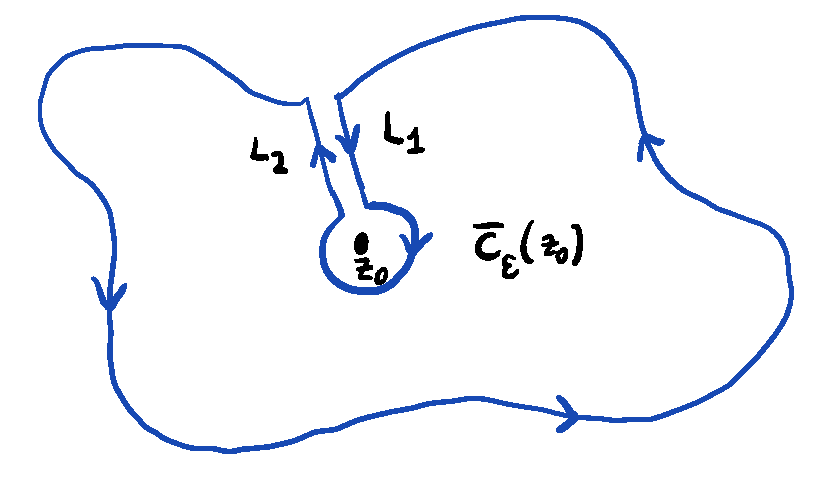
\includegraphics[width=\linewidth]{figs/cauchy_integral-cropped.pdf}
\caption{Contour $C'$ that excises the pole $z_0$ of the
function~\eqref{eq:simplePole}. Following the notation of
\propref{prp:circleIntegral}, $\overline{C}_{\epsilon}(z_0)$ is a circle of
radius $\epsilon$ centered on $z_0$, with the bar indicating that it has a CW
orientation.}
\label{fig:cauchy}
\end{figure}

We choose our excision to have arbitrarily small radius $\epsilon$.
In the limit $\epsilon\to0$, we have
\begin{equation}
  C'=\partial B + L_1 + \overline{C}_{\epsilon}(z_0) + L_2.
\end{equation}
In this limit, $L_1$ and $L_2$ will cancel since they have opposite
orientations.
We can now parameterize $z$ on $\overline{C}_{\epsilon}(z_0)$ 
by $z-z_0=\epsilon e^{i\phi}$, and putting everything together, we find
\begin{equation}\begin{aligned}\label{eq:cauchyn0}
  \oint_{\partial B}\dd{z}\frac{f(z)}{z-z_0}
&=-\lim_{\epsilon\to 0}\int_{2\pi}^0\dd{\phi}
     i\epsilon e^{i\phi}\frac{f(z_0+\epsilon e^{i\phi})}{\epsilon e^{i\phi}}\\
&=i\lim_{\epsilon\to 0}\int_{0}^{2\pi}\dd{\phi}f(z_0+\epsilon e^{i\phi})\\
&=i\int_{0}^{2\pi}\dd{\phi}f(z_0)\\
&=2\pi if(z_0).
\end{aligned}\end{equation}

\index{Cauchy!integral formula}
\begin{theorem}{Cauchy integral formula}{}
Let $B\subset\C$ be bounded and simply connected region. Let $f:B\to\C$ be
holomorphic in $B$ and continuous on the boundary $\partial B$.
Then $\Forall n\in\N$ we get
$$
  \oint_{\partial B}\dd{z}\frac{f(z)}{(z-z_0)^{n+1}}=
\begin{cases}
\frac{2\pi i}{n!}f^{(n)}(z_0) & z_0\in B \\
 0            & \text{otherwise}.
\end{cases}
$$
\begin{proof} When $z_0\notin B$, we get 0 by the Cauchy integral theorem.
Therefore we consider for the remainder of the proof $z_0\in B$.
The $n=0$ case is given by \equatref{eq:cauchyn0}. 
From here, all one has to do is take partial derivatives of this result 
w.r.t. $z_0$.
\end{proof} 
\end{theorem}

\section{The residue theorem}\index{residue!theorem}\label{sec:residueThm}

Let $f$ be holomorphic in the annulus ${z\in\C : 0\leq r<|z-z_0|<R}$
where $r,R>0$.
Define $\Forall\rho : r<\rho<R$ and $\Forall k\in\Z$
\begin{equation}\label{eq:laurentCoeff}
  a_k\equiv\frac{1}{2\pi i}\oint_{C_{\rho}(z_0)}\dd{z}\frac{f(z)}{(z-z_0)^{k+1}}.
\end{equation}
Then the {\it Laurent expansion}\index{Laurent expansion} of $f$ is
\begin{equation}\label{eq:laurentExpansion}
  f(z)=\sum_{k=-\infty}^\infty a_k(z-z_0)^k.
\end{equation}
The $a_k$ are unique and independent of $\rho$, and the Laurent expansion
defines $f$ in the annulus.
If $f$ permits a Taylor expansion, this Taylor series is the Laurent
series, with $a_k=0$ whenever $k<0$.

To get some intuition for why this is true, we can at least show that the
definition~\eqref{eq:laurentCoeff} is consistent.
Plugging \equatref{eq:laurentExpansion} into \equatref{eq:laurentCoeff}
and applying the Cauchy integral formula, we find
\begin{equation}
  a_k\equiv\frac{1}{2\pi i}\sum_{l=-\infty}^\infty\oint_{C_{\rho}(z_0)}
  \dd{z}\frac{a_l}{(z-z_0)^{k-l+1}}
     = \sum_{l=-\infty}^\infty a_l\delta_{k-l,0}=a_k.
\end{equation}

Laurent series can also be used to classify the isolated singularities
of \secref{sec:complexPrelim}. In particular $f$ has at $z_0$
\begin{itemize}
  \item a removable singularity if $a_k=0$ $\Forall k<0$;
  \item a pole of order $m$ if the first, non-vanishing coefficient
        is $a_{-m}$; and
  \item an essential singularity if there is no first, non-vanishing
        coefficient $a_{-m}$.
\end{itemize}

Suppose $f$ has a Laurent expansion in an annulus about $z_0$.
Then the\index{residue} {\it residue} of $f$ at $z_0$ is
\begin{equation}
 \Res f(z_0)=a_{-1}=\frac{1}{2\pi i}\oint_{C_{\rho}(z_0)}\dd{z}f(z).
\end{equation}

\begin{figure}
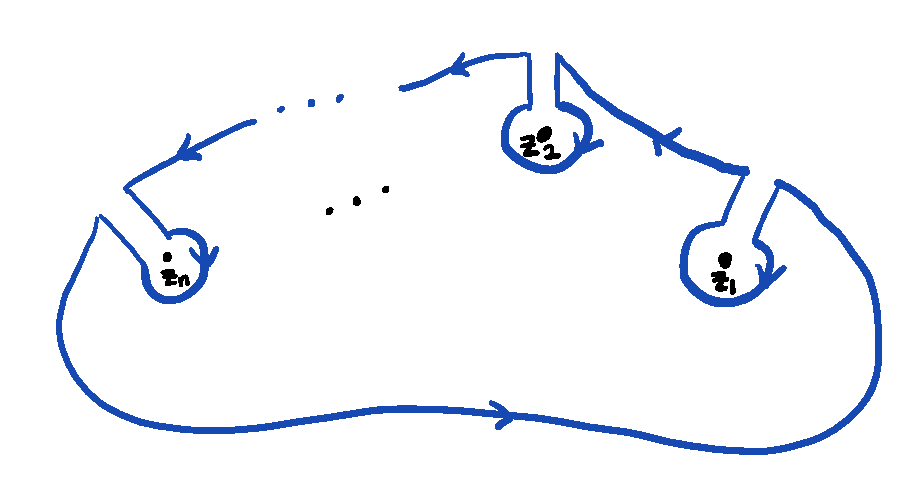
\includegraphics[width=\linewidth]{figs/residue_theorem-cropped.pdf}
\caption{Contour $C'$ that excises all isolated singularities of
the residue theorem. Each singularity is excised by the circle
$\overline{C}_{\rho_k}(z_k)$.}
\label{fig:residue}
\end{figure}

\begin{theorem}{Residue theorem}{residueThm}
Let $B\subset\C$ be an area bounded by a finite number of piecewise
continuous curves. Let $f$ be holomorphic on $\partial B$ 
holomorphic in $B$, except for a finite number of isolated 
singularities $z_1$, ..., $z_n\in B$. Then
$$
\oint_{\partial B}\dd{z}f(z)=2\pi i\sum_{k=1}^n\Res f(z_k).
$$
\begin{proof}
We construct the contour $C'$ indicated in \figref{fig:residue}
created by excising the singularities. Each singularity is
excised with contour $\overline{C}_{\rho_k}(z_k)$, with the
radius $\rho_k$ chosen such that the Laurent expansion
of $f$ converges there. To complete the proof, we use the Laurent
expansion of $f$ around each singularity.
\begin{equation*}
  \oint\dd{z}f(z)=\sum_{k=1}^n\sum_{l=-\infty}^\infty 
                    a_l^{(k)}\oint_{C_{\rho_k}(z_k)}(z-z_k)^l.
\end{equation*}
According to \propref{prp:circleIntegral}, each integral will contribute 
only if $l=-1$; there it contributes $2\pi i$. That the residue is
$a_{-1}$ by definition completes the proof.
\end{proof}
\end{theorem}

\begin{figure}
\centering
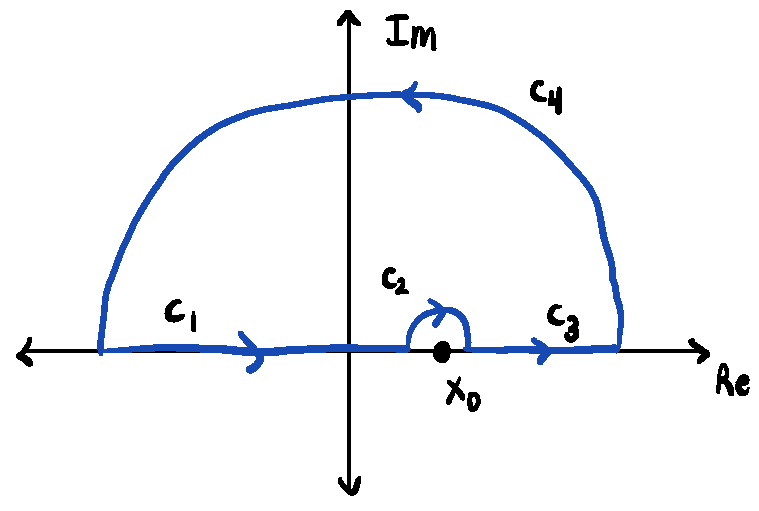
\includegraphics[width=0.75\linewidth]{figs/principal_value-cropped.pdf}
\caption{Example contour used to assign a principal value to a real integral.
Here the semicircle $c_2$ has radius $\epsilon$ and excises the singularity
$x_0$ on the real axis. The semicircle $c_4$ has radius $R$, and the function 
$f$ is asked to decay sufficiently quickly so that the contribution on 
$c_4$ will vanish as $R\to\infty$.}
\label{fig:principalValue}
\end{figure}

The residue theorem is extremely powerful for the evaluation of many integrals,
including real-valued ones. In particular it can be used to assign a number to
a sum of separately divergent, real-valued integrals. 
We begin with an example 
that does not require the residue theorem:
\begin{equation}\label{eq:principalEasy}
  \principal\int_{-a}^a\dd{x}\frac{1}{x}=0
\end{equation} 
with $a>0$, which you can convince yourself of since the integrand is odd. On
the other hand, if one were to split this into a contribution over negative and
positive numbers, each contribution would diverge.

In the above we have introduced the {\it principal value}\index{principal value}
symbol $\principal$. More formally let $f$ be defined in the interval $[a,b]$
with the possible exception $c$, $a<c<b$. Then 
\begin{equation}
  \principal\int_a^b\dd{x}f(x)\equiv\lim_{\epsilon\to0}
     \left(\int_a^{c-\epsilon}\dd{x}f(x)+\int_{c+\epsilon}^b\dd{x}f(x)\right).
\end{equation}

The example~\eqref{eq:principalEasy} was pretty straightforward. A more
interesting example would be
\begin{equation}
  \frac{f(x)}{x-x_0},
\end{equation}
where $f(z)$, $z=x+iy$, has no poles on the real axis. We will also require $f$
to decay in absolute value sufficiently quickly as we move away from the origin.
To determine the principal value, we can use a contour like the one
shown\footnote{If you like, you can also choose $c_2$ to close below the real
axis. Then the singularity $x_0$ will have to be considered in your residue
theorem. The result is the same in either case.}
in \figref{fig:principalValue}. The contours $c_1$ and $c_3$ combine to give
the principal value, and we therefore have by the residue theorem
\begin{equation}
  \principal\int_{-\infty}^{\infty}\dd{x}\frac{f(x)}{x-x_0}
   +\left(\int_{c_2}+\int_{c_4}\right)\dd{z}\frac{f(z)}{z-x_0}
   =2\pi i\sum_k\Res \frac{f(z_k)}{z_k-x_0}. 
\end{equation}
If $f$ decays fast enough, it will vanish on $c_4$, so that term can be
neglected. It remains to evaluate $f$ on $c_2$. We find
\begin{equation}
 \int_{c_2}\dd{z}\frac{f(z)}{z-x_0}
  =\lim_{\epsilon\to0}i\epsilon\int_\pi^0\dd{\phi}
      \frac{f(x_0+\epsilon e^{i\phi})}{\epsilon e^{i\phi}}=-\pi i f(x_0),
\end{equation}
and consequently,
\begin{equation}
  \principal\int_{-\infty}^{\infty}\dd{x}\frac{f(x)}{x-x_0}
   =\pi i f(x_0)+2\pi i\sum_k\Res \frac{f(z_k)}{z_k-x_0}. 
\end{equation}

In the special case where $f$ is analytic in the upper half plane,
there are no residues, and hence
\begin{equation}
  f(x_0)=\frac{1}{\pi i}\,\principal
     \int_{-\infty}^{\infty}\dd{x}\frac{f(x)}{x-x_0}.
\end{equation}
If we write $f(x)=\Re f(x)+i\Im f(x)$, we get from the above
\begin{equation}\begin{aligned}\label{eq:kramerKronig}
\Re f(x_0)&=\frac{1}{\pi}\,\principal
     \int_{-\infty}^{\infty}\dd{x}\frac{\Im f(x)}{x-x_0}\\
\Im f(x_0)&=-\frac{1}{\pi}\,\principal
     \int_{-\infty}^{\infty}\dd{x}\frac{\Re f(x)}{x-x_0}.
\end{aligned}\end{equation}
We call \equatref{eq:kramerKronig} the 
{\it Kramers-Kronig relations}.\index{Kramers-Kronig relations}
They show that the real and imaginary parts of a function $f$ with the given
properties are closely related to each other along the real line.


\section{The Riemann sphere}\index{Riemann sphere}


In this section we introduce a projection of the complex plane called the {\it
Riemann sphere}. It is shown in \figref{fig:riemann}.
The complex plane bisects the Riemann sphere, which is a sphere of unit radius,
and we define a bijective mapping from every point of the $\C$ to the sphere as
follows: Let $(\xi,\eta,\zeta)$ be the coordinates on the surface of the sphere
with respect to its center, so that $\xi^2+\eta^2+\zeta^2=1$.
Then by geometry,
\begin{equation}\label{eq:planeToSphere}
  z=\frac{\xi+i\eta}{1-\zeta},~~~~~~
  \xi+i\eta=\frac{2z}{1+|z|^2},~~~~~~~
  \zeta=\frac{|z|^2-1}{|z|^2+1}.
\end{equation}
The opposite end of a diameter through $(\xi,\eta,\zeta)$ is
$(-\xi,-\eta,-\zeta)$, which corresponds $-1/z^*$.

It is useful to introduce an idea of distance on the Riemann sphere.
A natural choice is the chord length between two points $z$ and $w$
projected onto the sphere. From \equatref{eq:planeToSphere} 
the chord length on the sphere is
\begin{equation}
  D^2(z,w)=\frac{4|z-w|^2}{|1+z^*w|^2+|z-w|^2}.
\end{equation}
This distance satisfies $0<D\leq2$, 
which means we can also about distances to infinity.

This definition of distance can be used to characterize convergence of a
sequence of complex numbers on the sphere. In particular 
a sequence of complex numbers $z_n$ is said to\index{converge!on the sphere}
{\it converge on the sphere} if $\Forall\epsilon>0$ $\Exists N\in\N$
such that
\begin{equation}
  D^2(z_n,z_m)\leq\epsilon^2
\end{equation}
$\Forall n,m\geq N$.

\begin{figure}
\centering
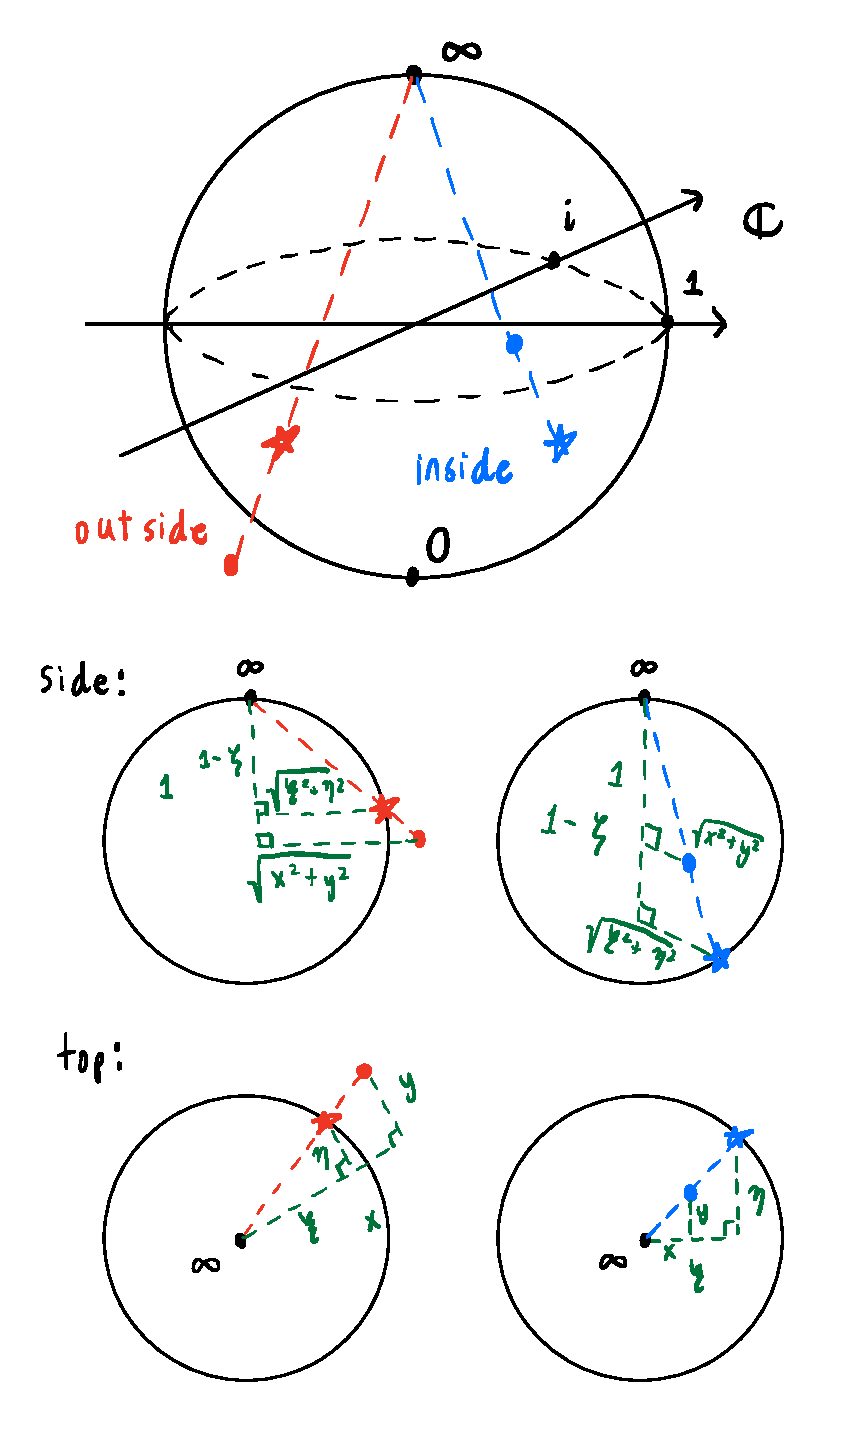
\includegraphics[width=0.7\linewidth]{figs/riemann.pdf}
\caption{{\it Top}: Example mappings of the complex plane to the Riemann sphere.
Filled dots indicate points on the complex planes and stars indicate points on
the surface of the sphere. Hence red lines pierce the sphere and land outside,
while blue lines terminate on the surface. {\it Middle}: A side view of the
Riemann sphere, along with similar triangles to map coordinates on the complex
plane to coordinates on the sphere. {\it Bottom}: Top view of the Riemann
sphere.}
\label{fig:riemann}
\end{figure}


\section{Pad\'e approximants}\index{Pad\'e approximant}

To define the Pad\'e approximant, we introduce\footnote{One can always force
the first coefficient in the denominator to be 1 by factoring it out of all
the other coefficients in both the numerator and denominator.} first the {\it rational
function of order} $[m,n]$, $m,n\in\N$ as \index{function!rational}
\begin{equation}
  R_n^m(x)\equiv\frac{\sum_{i=0}^m a_ix^i}{1+\sum_{j=1}^nb_jx^j}.
\end{equation}
Rational functions can be used instead of Taylor series to approximate
functions with low numbers of terms. They sometimes may have a larger range of
validity than a truncated Taylor series: The intuition is that the coefficients
in the denominator capture some of the contributions from higher order terms.

Let $f$ have a formal Taylor series
\begin{equation}
  f(x)=\sum_{i=0}^\infty c_kx^k.
\end{equation}
Then the {\it Pad\'e approximant} of order $[m,n]$ is the rational function
$R_n^m$ with coefficients so that
\begin{enumerate}
  \item there are no common factors between the numerator and denominator
  \item and it equals the Taylor series up to order $m+n$.
\end{enumerate}
This definition gives a relationship between the coefficients $a_i$, $b_j$, and
$c_k$. We will use this to characterize in which sense Pad\'e approximants
converge to the function they approximate.

Sometimes one does not have access to higher order Taylor coefficients.
One can introduce further constraints by asking that a Pad\'e approximant to agree
with the Taylor series at multiple points, which can be useful if it's easier to
determine lower orders at multiple points than a higher order at a single
one\footnote{This is the situation for lattice determinations of the QCD
pressure expansion in $\mu_B/T$.}. This is the so-called
{\it multi-point Pad\'e}\index{Pad\'e approximant!multi-point}.

\subsection{Rigorous properties}

Here we collect a few known, easy to understand 
facts about Pad\'e approximants. For proofs, we refer
the reader to Ref.~\cite{baker_essentials_1975}. This thorough reference also
contains other useful rigorous properties of Pad\'es. A more up-to-date, brief
article about Pad\'es by the same author can be found in
Ref.~\cite{Jr:2012}.

\begin{theorem}{Uniqueness}{padeUniq}
When it exists, the $[m,n]$ Pad\'e approximant to any Taylor series is unique.
\end{theorem}

\begin{theorem}{Existence}{padeExist}
Given any formal power series with $c_0\neq0$,
then: $\Forall n\in\N$ there exists an infinite sequence of $m_j$ for which the
$[m_j,n]$ Pad\'e exists; $\Forall m\in\N$ there exists an infinite sequence of $n_j$ for
which the $[m,n_j]$ Pad\'e exists; and $\Forall q\in\N$ there exists an infinite
sequence of $m_j$ for which the $[m_j + q/m_j]$ Pad\'e exists.
\end{theorem}

\begin{theorem}{Montessus de Ballore's Theorem}{}
Let $f(z)$ be regular inside the circle $|z|<R$ except for poles of total
multiplicity $n$. Then $\Forall R>0$
the $[m,n]$ Pad\'e converges uniformly
to $f(z)$ on the sphere in $|z|\leq R$ as $m\to\infty$.
\end{theorem}

Montessus de Ballore's theorem guarantees convergence of Pad\'es for meromorphic
functions. It is desirable to use Pad\'es in contexts where functions have more
exotic singularities, for example functions with essential singularities and
branch cuts. Unfortunately it is hard to find practical, rigorous results for
these. For these issues we use numerical experiments to try to glean a few
intuitive or apparent, empirical properties. 


\subsection{Unrigorous properties}



Pad\'e approximants are continuous, except at their poles. That it makes sense
to represent functions with simple poles using Pad\'e approximants is guaranteed
by Montessus de Ballore's theorem. On the other hand,
there may be cases where one constructs a Pad\'e approximant for a function with
an essential singularity or a branch cut, and one may wonder how such
singularities manifest in the approximant.

Since Pad\'e approximants are continuous except at their poles, it must be that
all singularities are somehow represented by poles in the approximant. An
essential singularity, which is an isolated singularity, is represented by a
pole in the approximant. The more interesting case is the branch cut; the only
way the Pad\'e can feel the cut is by a line of poles. The number of points
along the cut is limited by the order $n$ of the $[m,n]$ approximant, and the
rough intuition is that cut is ``recovered" as $n\to\infty$.



\bibliographystyle{unsrtnat}
\bibliography{bibliography}

%\chapter{Math: Differential Geometry}
\section{Topological manifolds}
Why should a physicist care about topology? Frederic Schuller gave a good
motivation for learning topology in the 2015 Winter School on Gravity and
Light~\cite{schuller}: we need to be able to speak sensibly about 
continuity in the most general way possible. In particular, we need 
to understand what it means for maps between manifolds to be continuous.  
Let $M$ be a set. A {\it topology on $M$}\index{topology} is a subset
$\topol{M}\subset2^M$ satisfying
\begin{enumerate}
  \item $\emptyset,M\in\topol{M}$;
  \item $U\in\topol{M}$ and $V\in\topol{M}$ $\Rightarrow
         U\cap V\in\topol{M}$; and
  \item $\{U_\alpha\}\in\topol{M}\Rightarrow
           \bigcup\limits_\alpha U_\alpha\in\topol{M}$.
\end{enumerate}
A {\it topological space}\index{topological!space} is a pair 
$(M,\topol{M})$. The sets $U$ are said to be {\it open}\index{set!open}, 
while a set $A$ is said to be {\it closed}\index{set!closed} if
and only if $M-A$ is open.

\begin{example*}{}{}
  \leavevmode
  \begin{enumerate}
    \item For any set $M$, the {\it chaotic topology}\index{topology!chaotic} 
          is given by $\topol{\text{chaotic}}=\{\emptyset,M\}$. On the 
          opposite end of the spectrum, the {\it discrete topology}
          \index{topology!discrete} is simply $\topol{\text{discrete}}=2^M$.
    \item Consider $\mathbb{R}^n$ equipped with the Euclidean metric. The
          {\it standard topology} \index{topology!standard} is 
          $$\topol{\text{standard}}=
          \{U\in2^{\mathbb{R}^n}:\Forall p\in U,\ \Exists r>0\ 
          \text{with}\ B_r(p)\in U\}.$$ Note in this case that the topological
          definition of open set agrees with the definition that relies
          on limit points.
  \end{enumerate}
\end{example*}
Let $(M,\topol{M})$ and $(N,\topol{N})$ be topological spaces. A mapping
$f:M\to N$ is {\it continuous}\index{map!continuous} if 
$\Forall V\in \topol{N}$, $f^{-1}(V)\in\topol{M}$.
In other words, continuous functions are those that guarantee that you started
off in an open set, if you ended up in an open set. Note that whether a
function is continuous depends on the topology.
\begin{theorem}{}{}
  Let $M$, $N$, and $P$ be open sets with respective topologies and suppose
  $f:M\to N$ and $g:N\to P$ are continuous. Then $g\circ f:M\to P$ is
  continuous.
  \begin{proof}
    We need to check that the preimage of $g\circ f$ is open. Note
    \begin{equation*}
    \begin{aligned}
      (g\circ f)^{-1}(P)&=\{m\in M:g\circ f(m)\in P\}\\
        &=\{m\in M:f(m)\in g^{-1}(P)\}\\
        &=f^{-1}(g^{-1}(P)).
    \end{aligned}
    \end{equation*}
    Since $g$ is continuous, $g^{-1}(P)$ is open. It follows by
    the continuity of $f$ that $f^{-1}(g^{-1}(P))$ is open,
    which completes the proof.
  \end{proof}
\end{theorem}
Hence the composition of continuous functions is continuous, which is what
you learned in calculus. Using the definition of continuity, we can know
determine when two topological spaces are, in some sense, equivalent.
A map between two topological spaces $f:M\to N$ is called a 
{\it homeomorphism}\index{map!homeomorphic} if
\begin{enumerate}
  \item $f$ is invertible;
  \item $f$ is continuous with respect to the topologies of $M$ and $N$; and
  \item $f^{-1}$ is also continuous.
\end{enumerate}
If such a function exists, we say $M$ and $N$ are {\it homeomorphic}.
So for example when a topological space is homeomorphic to
$\mathbb{R}^d$, that topological space is essentially a warped version
of $\mathbb{R}^d$. Also given a topological space, we can always make another
one from a subset of that space. In fact
\begin{proposition}{}{}
  Let $(M,\topol{M})$ be a topological space. Let $S\subseteq M$ and
  $\topol{M}|_S\subseteq 2^S$ such that 
  $\topol{M}|_S=\{U\cap S:U\in\topol{M}\}$. Then $(S,\topol{M}|_S)$ forms
  a topological space.
\end{proposition}
Let $d\in\mathbb{N}$. A topological space $(M,\topol{M})$ is called a
{\it topological manifold of dimension d}\index{manifold} if $\Forall x\in M$, 
$\Exists U$ containing $x$ that is homeomorphic to $\mathbb{R}^d$. Here
$\mathbb{R}^d$ is taken with the standard topology. We say:
\begin{enumerate}\index{chart}\index{atlas}\index{map!chart}
  \item $(U,f)$ is a {\it chart} of $(M,\topol{M})$.
  \item An {\it atlas} $\mathcal{A}$ is a collection of charts
        $(U_\alpha,f_\alpha)$ such that $M=\bigcup_\alpha U_\alpha$.
  \item Sometimes we call the homeomorphism for each chart a
        {\it chart map}.
\end{enumerate}
Clearly mathematicians got carried away with sailing analogies. But I think
they make the meaning of the terminology easy to remember. Now let's say that
I have two charts $(U_x,f)$ and $(U_y,g)$ of points $x$ and $y$ in the
manifold, and suppose further they overlap, i.e. $U_x\cap U_y\neq\emptyset$.
Consider a point $z$ in the intersection. Each chart gives me a perfectly
reasonable representation of $z$. How can I easily translate from one to the
other? Well, since $f$ and $g$ are invertible by definition the map
$$g\circ f^{-1}:f(U_x\cap U_y)\to g(U_x\cap U_y)$$
will do the trick.\index{map!chart transition}
$g\circ f^{-1}$ is called the {\it chart transition map}.
Informally, the chart transition map tells you how the charts of an atlas meld
together to form the manifold. It's also useful in the following sense: We
want to be able to do things, such as judging whether a path is continuous, by
only looking at charts. If we look at a chart and find that it is continuous,
can we guarantee that the path is as well? Because of the chart transition
map, we can. Let's call the path $\gamma$ and let $f$ and $g$ be two chart
maps. Now suppose we find that $f\circ\gamma$ is continuous. Then it follows
that $g\circ\gamma=g\circ f^{-1}\circ f\circ\gamma$ is continuous. Hence we 
know that we can define continuity of $\gamma$ in this way, that this is a
well-defined notion, because this notion does not depend on our choice of
chart map.

\section{Multilinear algebra}
Let $V$ and $W$ be vector spaces.
The set of linear maps from $V$ to $W$ is denoted by Hom($V$,$W$).
\begin{proposition}{}{}
  \normalfont{Hom($V$,$W$)} forms a vector space under vector addition 
  and scalar multiplication operations of $W$. 
\end{proposition}
We will now learn about a very special vector space. Given $V$ along with
this new vector space, we will be able to construct many other vector spaces.
The {\it dual space}\index{dual space} 
is given by $V^*\equiv\text{Hom}(V,\mathbb{R})$.
An element of the dual space is called a {\it one-form} or {\it covector}.
\index{one-form}\index{covector}
Let $V$ be $n$-dimensional with basis $\{e^1,...,e^n\}$. If a basis
$\{\epsilon_1,...,\epsilon_n\}$ of $V^*$ satisfies
  $$\epsilon^a(e_b)=\delta^a_b$$
\index{dual basis}
then it is called the {\it dual basis} of $V^*$.
\begin{theorem}{}{}
  If \normalfont{dim}(V)$\;<\infty$, then $\big(V^*\big)^*=V$.
\end{theorem}
\begin{example*}{}{}
  Consider the 4D vector space of polynomials of degree 3 with
  real coefficients. A basis for this space is $\{1,x,x^2,x^3\}$. 
  The dual space is the set of mixed differential operators of order 3 or 
  smaller. It's not hard to see that the dual basis is 
  $$\Bigg\{1,\frac{\partial}{\partial x},
             \frac{1}{2}\frac{\partial^2}{\partial x^2},
             \frac{1}{6}\frac{\partial^3}{\partial x^3}\Bigg\}.$$
\end{example*}
Perhaps you encountered tensors in physics and were told something useless
like ``a tensor is an object that transforms like a tensor."
You will now get to see a more illuminating definition.
  Let $r,s\in\mathbb{N}$.\index{tensor}
  A {\it tensor of rank ($r$,$s$)} is a map
  $$T:\underbrace{V^*\times...\times V^*}_\text{$r$ times}\times
      \underbrace{V\times...\times V}_\text{$s$ times}\to\mathbb{R}$$
  that is linear in all its arguments.
In other words, a tensor is a multilinear map that eats
vectors and covectors and spits out a real number. Now, you may be used
to (1,1) tensors being objects that take vectors to vectors. Given
a tensor $T$, we can actually recover such a construction.
\begin{example*}{}{}
  Given a tensor $T:V^*\times V\to\mathbb{R}$, where $V$ is a vector space
  of finite dimension, define the map $\phi:V\to \big(V^*\big)^*=V$ by
  $$\phi(v)=T(\cdot,v),$$
  where $v\in V$ and the $\cdot$ represents an as-yet-unspecified covector. 
  We see that the RHS of the above equation is an element of $(V^*)^*$ 
  since it eats covectors and spits out real numbers. So the map $\phi$ takes
  a vector to a vector. Similarly if we 
  define the map $\phi:V^*\to V^*$ by
  $$\phi(\omega)=T(\omega,\cdot),$$
  where $\omega\in V^*$ and $\cdot$ is an as-yet-unspecified vector, we see
  $\phi$ takes a covector to a covector.
\end{example*}
\begin{example*}{}{}
 Here are some more familiar tensors:
  \begin{enumerate}
    \item Clearly rank (0,1) tensors are covectors, which is why they are 
          also called one-forms. Similarly rank (1,0) tensors are vectors.
    \item An inner product is a rank (0,2) tensor.
    \item The gradient is a rank (0,1) tensor.
  \end{enumerate}
\end{example*}
Again let $V$ be finite dimensional. Given a basis of $V$ and the corresponding
dual basis of $V^*$, we can write $\Forall v\in V$ and $\Forall \omega\in V^*$
\begin{equation}
  v=v^1e_1+...+v^ne_n,~~~\omega=\omega_1\epsilon^1+...+\omega_n\epsilon^n.
\end{equation}
That is, we can write $v$ in terms of its components $v^i$ and $\omega$ in
terms of its components $\omega_i$. We can do the same thing for tensors.
For a rank $(r,s)$ tensor, each component is given by
\begin{equation}
  T\indices{^{i_1...i_r}_{j_1...j_s}}
    =T(\omega^{i_1},...,\omega^{i_r},e_{j_1},...,e_{j_s}),
\end{equation}
where $1\leq i,j\leq n$.

\bibliographystyle{unsrtnat}
\bibliography{bibliography}


\chapter{Math: Probability and Statistics}

Crucial to the study of quantum physics, statistical physics, experiment, and
eventually lattice field theory is an understanding of probability and the
ability to understand statistics. These skills are actually quite important to
understand all modern science, not just physics, as well as in everyday
circumstances like politics.
You already have a rough idea of probability: It's a way of saying whether you
think something will happen or not, while in general signaling that you aren't
completely certain. We will now make these ideas precise.
Parts of this presentation follow selected parts
of Chapters~1 and~2 of Berg~\cite{berg_markov_2004}.


\section{Preliminaries}


We will consider a {\it random variable}\index{random variable}\footnote{
We will try to denote random variables by capital letters.} $X$ which
has some possible {\it outcomes}\index{outcome} $x_i$. The random variable will take
one of the values in $x_i$, but we don't know for sure which one.
The set of all possible outcomes
\begin{equation}
  \Omega=\{x_1,x_2,...,x_n\},
\end{equation}
assuming there are $n\in\N$ possible outcomes, is called the {\it sample
space}\index{sample space}. If $|\Omega|$ is finite as in the above case, we
say that $X$ is {\it discrete}\index{discrete}. An {\it event}\index{event} $E$
is any subset of outcomes $E\subset\Omega$, and we assign it a {\it
probability}\index{probability} $\pr{E}$. Axiomatically speaking, the
probability has to fulfill two conditions:
\begin{enumerate}
  \item $\Forall E$, $0\leq\pr{E}\leq1$.
  \item $\pr{\Omega}=1$, i.e. the random variable $X$ needs to have some outcome
in $\Omega$. Another way to state this is that the probability of at least one
of the possibilities is 1.
\end{enumerate}

Pragmatically you can assign a probability by repeating some experiment $n$
times. If the event $E$ occurs $n_E$ times, then
\begin{equation}
  \pr{E}\equiv\lim_{n\to\infty}\frac{n_E}{n}.
\end{equation}
Alternative, you can make some theoretical assignment of probabilities to
events. For instance when one tosses a coin, if one has no reason to believe the
coin is biased, it must be that
\begin{equation}
\pr{\text{heads}}=\pr{\text{tails}}=\frac{1}{2}.
\end{equation}
This theoretical assignment is nice, but it should eventually be checked against
some observation or measurement as well.
In the case that $|\Omega|<\infty$,
we might say that the probability of event $E$ is $\pr{E}=|E|/|\Omega|$. In
this instance, we say that the probability is {\it uniform}
\index{PDF!uniform} since every point in the sample space is equally likely. 


Sometimes the cardinality of $\Omega$ is uncountably infinite. For instance you
may ask something like: What is the probability that a particle in this gas has
a speed between $v_1$ and $v_2$? In this case, the sample space is
\begin{equation}
  \Omega=\{x\suchthat0\leq x\leq c\},
\end{equation}
where $c$ is the speed of light.
In such a case we speak of a {\it continuous} random variable $X$.
The probability that $X$ takes any one particular value in $\Omega$ is
zero\footnote{Intuitively you could ask yourself: What is the probability that
my speed is exactly $\pi$ to all infinitely many digits? When checking against
experiment, you will never be able to resolve all infinitely many digits, so at
best you must specify a range corresponding to the resolution of your
instrument. In formal mathematical language, we require $\Omega$ to be
{\it measurable}.}.
We can only assign
sensible probabilities to subsets of $\Omega$ of uncountably infinite
cardinality. In the above
case, this corresponds to the range of velocities between $v_1$ and $v_2$.
The probability that $X$ takes a value in the small range of velocities $\dd x$
is denoted
\begin{equation}
   \pr{X\in[x,x+\dd x]}=\dd{x}f(x),
\end{equation}
and hence for continuous random variables, the probability must instead
fulfill the properties
\begin{enumerate}
  \item  $0\leq\dd{x}f(x)\leq 1$ and
  \item $\int_{x\in\Omega}\dd{x}f(x)=1$.
\end{enumerate}
In general for some integrable function 
$f:\R\to\R$, we assign a 
probability that $X$ lies in the interval $[a,b]$ by
\begin{equation}
  \label{eq:cpr}
  \pr{X\in[a,b]}=\int_a^b\dd{x}f(x).
\end{equation}
For the remainder of this chapter, we will
only be concerned with continuous random variables, and we will simply call
them random variables.
The function $f$ is called the {\it probability distribution function} 
(PDF)\index{PDF}; meanwhile the {\it cumulative distribution function} 
(CDF) is the function\index{CDF} $F(x)$ given by
\begin{equation}
  F(x)\equiv \pr{X<x}=\int_{-\infty}^x\dd{t}f(t).
\end{equation}
\begin{example*}{}{}
Two examples of important probability distributions include the {\it Gaussian}
or {\it normal} distribution,\index{PDF!normal}
\begin{equation}
  \gau(x,\hat{x},\sigma)\equiv\frac{1}{\sigma\sqrt{2\pi}}
  \exp\Bigg(-\frac{(x-\hat{x})^2}{2\sigma^2}\Bigg)
\end{equation}
where $\sigma$ is the standard deviation of the distribution and $\hat{x}$ is 
the mean, and the {\it Cauchy} \index{PDF!Cauchy} distribution,
\begin{equation}
  \cau(x,\alpha)\equiv\frac{\alpha}{\pi\big(\alpha^2+x^2\big)}.
\end{equation}
I will refer to these special PDFs later, particularly the normal distribution.
I'll call their CDFs $\Gau$ and $\Cau$, respectively.   
\end{example*}

Now that we know what probabilities and PDFs are, we can start thinking about
ways to characterize them. For example we can think about typical values taken
by a random variable from some distribution. We can get some information
from the mean and variance of a distribution. These are
both special cases of a more general concept.
In particular, let $n\in\N$.
  The {\it $n\nth$ moment} \index{moment}of the distribution $f(x)$ is
  \begin{equation}\label{dfn:mom}
    \ev{X^n}=\int_{-\infty}^\infty\dd{x}x^nf(x).
  \end{equation}

The mean and variance are the special cases $\hat{x}=\ev{X}$ and 
$\sigma^2=\ev{(X-\hat{x})^2}$. Sometimes we call the mean the {\it expected
value} and sometimes we denote the variance $\variance$. Note that not all 
probability distributions have well-defined moments. The Cauchy distribution is
very ill-behaved in this regard, since its $n\nth$ moment diverges
$\Forall n\in\N$.
Generally in the lab, one draws random variables from distributions
about which one has no a priori knowledge. Therefore in principle one
doesn't know the true moments these distributions. The
definition \eqref{dfn:mom} suggests a way to estimate them. 
Suppose you draw a sample $X_1,...,X_N$:
  An {\it estimator}\index{estimator} of the $n\nth$ moment is
  \begin{equation}
    \bar{X}^n\equiv\frac{1}{N}\sum_{i=1}^N X_i^n.
  \end{equation}
In the case $n=1$ we obtain the ordinary arithmetic average.
We use the hat to distinguish true values from estimators, which will
generally be denoted with a bar. For estimators of moments besides the
mean, we must be more careful; this is discussed in \secref{sec:bias}.

Consider two intervals $[a,b]$ and $[c,d]$ and two random variables
$X$ and $Y$ drawn from PDFs $f$ and $g$, respectively. Then $X$ and $Y$ are
said to be {\it independent}\index{random variable!independent} if
\begin{equation}\label{dfn:ind}
  \pr{X\in[a,b]\text{ and }Y\in[c,d]}=\int_a^b\int_c^d\dd{x}\dd{y}f(x)\,g(y)
\end{equation}
Hence we see that the {\it joint PDF}\index{PDF!joint} of $X$ and $Y$ 
is $f(x)g(y)$. On the other hand, we say $X$ and $Y$ are {\it uncorrelated} 
\index{random variable!uncorrelated} if
\begin{equation}
  \ev{XY}=\ev{X}\ev{Y},
\end{equation}
The {\it covariance}\index{covariance}
\begin{equation}\label{dfn:cov}
  \Cov[X,Y]\equiv\ev{XY}-\ev{X}\ev{Y}
\end{equation}
can be used to give a measure of how correlated $X$ and $Y$ are, or
one can use the {\it correlation}\index{correlation}
\begin{equation}\label{dfn:cor}
  \rho(X,Y)=\frac{\Cov[X,Y]}{\sigma_X\sigma_Y}.
\end{equation}
So equivalently we say $X$ and $Y$ are correlated if $\rho(X,Y)=0$.
It's worth emphasizing that if $X$ and $Y$ are independent,
it follows that they are uncorrelated. This can be seen by applying
definition \eqref{dfn:mom} to the random variable $XY$, then using
definition \eqref{dfn:ind}. However if $X$ and $Y$ are
uncorrelated, {\it they can still be dependent}.
\begin{example*}{}{}
  Here's an extreme example by Cosma Shalizi~\cite{cosma_indep}. 
Let $X$ be uniformly distributed
  on [-1,1] and let $Y=|X|$. Then clearly $Y$ depends on $X$. However it 
  is easy to see that $Y$ is uniform on [0,1] and $\ev{XY}=0=\ev{X}\ev{Y}$. 
  Hence $X$ and $Y$ are not correlated.
\end{example*}

The next two propositions show us how to add expectation values and
random variables. Let $X$ and $Y$ be independent random variables 
drawn from PDFs $f$ and $g$, respectively.
\begin{proposition}{}{}
  Let $a,b\in\R$ be constants. Then
  $$\ev{aX+bY}=a\ev{X}+b\ev{Y}.$$
  \begin{proof}
    Since $X$ and $Y$ are independent, their joint PDF is $fg$. Then
    \begin{equation*}
      \begin{aligned}
      \ev{aX+bY}&=\int\dd{x}\dd{y}(ax+by)f(x)g(y)\\
                &=a\int\dd{x}\dd{y}x\,f(x)g(y)+
                 b\int\dd{x}\dd{y}y\,f(x)g(y)\\
                &=a\int\dd{x}x\,f(x)+b\int\dd{y}y\,g(y)\\
                &=a\ev{X}+b\ev{Y}.
      \end{aligned}
    \end{equation*}
  \end{proof}
\end{proposition}

\begin{proposition}{}{addvars}
  The PDF of the random variable $Z=X+Y$ is given by the convolution
  \begin{equation*}
    h(z)=\int_{-\infty}^\infty\dd{x}f(x)g(z-x)
  \end{equation*}
  \begin{proof}
    The CDF of $Y$ is, according to \equatref{dfn:ind},
    \begin{equation*}
      H(y)=\int_{x+y\leq z}\dd{x}\dd{y}f(x)g(y)
          =\int_{-\infty}^\infty\dd{x}f(x)\int_{-\infty}^{z-x}
            \dd{y}g(y).
    \end{equation*}
    The PDF $h$ follows from the Fundamental Theorem of Calculus:
    \begin{equation*}
      h(z)=\dv{H}{z}=\dv{H}{(z-x)}
          =\int_{-\infty}^\infty\dd{x}f(x)g(z-x).
    \end{equation*}
  \end{proof}
\end{proposition}

A sequence $\{X_N\}$ of random variables 
\index{converge!in probability}{\it converges in probability}
toward the random variable $X$ if $\Forall\epsilon>0$ 
\begin{equation}
  \lim_{N\to\infty}\pr{|X_N-X|>\epsilon}=0,
\end{equation}
and we write
\begin{equation}
  X_N\xrightarrow{\text{P}}X.
\end{equation}
The sequence converges to $X$ 
\index{converge!almost surely}{\it almost surely} if
\begin{equation}
  \lim_{N\to\infty}\pr{X_N=X}=1,
\end{equation}
and in this case we write
\begin{equation}
  X_N\xrightarrow{\text{AS}}X.
\end{equation}

\index{Chebyshev's inequality}
\begin{theorem}{Chebyshev's inequality}{}
  \index{Chebyshev's inequality}
  Let $X$ be drawn from a PDF with mean $\hat{x}$ and variance
  $\sigma^2$ and let $a>0$. Then
  \begin{equation*}
    \pr{|X-\hat{x}|>a\sigma}<a^{-2}.
  \end{equation*}
  \begin{proof}
    Let $T=(X-\hat{x})^2$ be a new random variable with PDF $g$. Then
    \begin{equation*}
      \pr{|X-\hat{x}|>a\sigma}=\pr{T>a^2\sigma^2}
                              =\int_{a^2\sigma^2}^\infty\dd{t}g(t)
    \end{equation*}
    But
    \begin{equation*}
      \begin{aligned}
        \sigma^2&=\int_{0}^\infty\dd{t}t\,g(t)
                =\Bigg(\int_0^{a^2\sigma^2}
                     +\int_{a^2\sigma^2}^\infty\Bigg)\dd{t}t\,g(t)\\
                &\geq\int_{a^2\sigma^2}^\infty\dd{t}t\,g(t)
                >a^2\sigma^2\int_{a^2\sigma^2}^\infty\dd{t}g(t)
                =a^2\sigma^2\pr{T>a^2\sigma^2}.
      \end{aligned}
    \end{equation*}
   Dividing through by $a^2\sigma^2$ completes the proof.
  \end{proof} 
\end{theorem}
Chebyshev's inequality tells you that large deviations from the mean are
unlikely. Intuitively you expect that as the number of measurements
increases, the sample average tends toward the true mean. This is
called the {\it Law of Large Numbers}\index{LLN}
(LLN). To prove it, we set up as follows: Let $X_1,...,X_N$ be a sequence 
of random variables drawn from a PDF
with mean $\hat{x}$ and variance $\sigma^2$.
\begin{theorem}{Weak LLN}{}
  $$
    \bar{X}\xrightarrow{\text{P}}\hat{x}.
  $$
  \begin{proof} Our proof will rely on Chebyshev's inequality, so we will
    first need to compute the mean and variance of the distribution of
    $\bar{X}$. All the $X_i$ are drawn from the same PDF, so
    $$
      \ev{\bar{X}}=\frac{1}{N}\sum_{i=1}^N\ev{X_i}
                  =\frac{N\hat{x}}{N}=\hat{x}.
    $$
    Meanwhile the variance of the distribution of $\bar{X}$ is
    $$
      \sigma^2_{\bar{X}}
      =\variance\sum_{i=1}^N \frac{X_i}{N}
      =\sum_{i=1}^N\frac{\sigma^2}{N^2}
      =\frac{\sigma^2}{N}.
    $$
    Now let $\epsilon>0$. Then $\exists\,a>0$ with 
    $\epsilon=a\,\sigma_{\bar{X}}$. Hence by Chebyshev's
    inequality we have
    $$
      \lim_{N\to\infty}\pr{|\bar{X}-\hat{x}|>\epsilon}
       \leq\lim_{N\to\infty}\frac{\sigma^2_{\bar{X}}}{\epsilon^2}
       =\lim_{N\to\infty}\frac{\sigma^2}{N\epsilon^2}=0.
    $$
    The probability can't be less than 0, so we're done.
  \end{proof}
\end{theorem}
The above proof relies on the PDF having a finite
variance. As it turns out, the Weak LLN is true
even when the variance is infinite! This can be proved
using characteristic functions. But since we don't introduce characteristic
functions until \secref{sec:CLT}, and since we assume in practice
that our data are drawn from PDFs with finite variance anyway,
we direct the reader elsewhere. For example, a proof can be
found on Wikipedia~\cite{Wiki_LLN}.

For completeness we also list the Strong LLN, but without proof. 
Like the Weak LLN, the Strong LLN is true even when the PDF variance
is infinite.

\begin{theorem}{Strong LLN}{}
  $$
    \bar{X}\xrightarrow{\text{AS}}\hat{x}.
  $$
\end{theorem}

Also in this section we list a sometimes useful fact about CDFs, which is
for example helpful in interpreting the results of some statistical
tests. (See e.g. \thmref{thm:gaudif}.) 

\begin{proposition}{}{}
  If a random variable $X$ is distributed according to the PDF $f$, then
  the corresponding CDF $F$ is distributed uniformly in [0,1].
  \begin{proof}
    If a random variable $Y$ is distributed uniformly in [0,1], then
    by definition we have $\Forall r\in [0,1]$
    $$
      \pr{0\leq Y\leq r}=r.
    $$
    So all we have to do is show that $F(X)$ behaves like $Y$. To that end,
    let $r\in[0,1]$ and define $X^*\in\R$ by
    $$
      r=\int_\infty^{X^*}\dd{s}f(s).
    $$
    Then
    $$
      \pr{0\leq F(X)\leq r}
      =\pr{-\infty\leq X\leq X^*}
      =\int_{-\infty}^{X^*}\dd{s}f(s)
      =r.
    $$
  \end{proof}
\end{proposition}

\section{The normal distribution}
\index{PDF!normal}
Now we're going to focus on results about the normal distribution specifically.
This first proposition will aid us in some of the calculations.

\begin{proposition}{}{gauss}
  Let $\alpha>0$. Then
  \begin{equation*}
    \int_{-\infty}^\infty\dd{x}e^{-\alpha x^2}=\sqrt{\frac{\pi}{\alpha}}.
  \end{equation*}
  \begin{proof}
    The trick is to just square the LHS:
    \begin{equation*}\begin{aligned}
      \left(\int_{-\infty}^\infty\dd{x}e^{-\alpha x^2}\right)^2
      &=\int_{-\infty}^\infty\int_{-\infty}^\infty\dd{x}\dd{y}
        e^{-\alpha(x^2+y^2)}\\
      &=\int_0^\infty \dd{r}r\int_0^{2\pi}\dd{\theta}e^{-\alpha r^2}\\
      &=\frac{\pi}{\alpha}.
    \end{aligned}\end{equation*}
  \end{proof}
\end{proposition}

For the next result 
let $X_1$ and $X_2$ be two independent random variables drawn from normal
distributions with respective means $\hat{x}_1$ and $\hat{x}_2$ and
standard deviations $\sigma_1$ and $\sigma_2$. 
\begin{proposition}{}{addgauss}
  The random variable $Y=X_1+X_2$ is normally distributed with mean
  $\hat{x}_1+\hat{x}_2$ and variance $\sigma_1^2+\sigma_2^2$.
  \begin{proof}
    By \propref{prp:addvars}, the sum $Y$ has the distribution
    \begin{equation*}
      g(y)=\frac{1}{2\pi\sigma_1\sigma_2}
           \int_{-\infty}^\infty\dd{x}\exp\left[
             -\frac{(x-\hat{x}_1)^2}{2\sigma_1^2}
             -\frac{(y-x-\hat{x}_2)^2}{2\sigma_2^2}\right].
    \end{equation*}
    Pull everything out of the integral that doesn't depend on $x$,
    then complete the square with what's left over.
    One obtains for $g(y)$
    $$
      \frac{1}{2\pi\sigma_1\sigma_2}
           \exp\left[-\frac{(y-\hat{x}_1-\hat{x}_2)^2}
                      {2(\sigma_1^2+\sigma_2^2)}\right]
           \int_{-\infty}^\infty\dd{x}
           \exp\left[-\frac{\sigma_1^2+\sigma_2^2}
                     {2\sigma_1^2\sigma_2^2}(x+C)^2\right],
    $$
    where $C$ is just a bunch of stuff that doesn't depend on $x$.
    Therefore you can make the substitution $u=x+C$ with $\dd u=\dd x$ and
    carry out the new integral using \propref{prp:gauss}.
    The result is
    \begin{equation*}
      g(y)=\frac{1}{\sqrt{2\pi(\sigma_1^2+\sigma_2^2)}}
           \exp\left[-\frac{(y-\hat{x}_1-\hat{x}_2)^2}
                      {2(\sigma_1^2+\sigma_2^2)}\right].
    \end{equation*}
  \end{proof}
\end{proposition}

Since the normal distribution is so important, so must be its CDF.
Unfortunately the integral of the normal PDF is {\it non-elementary};
\index{non-elementary} that is, it can't be expressed in terms of 
polynomials or standard
functions like $\sin$, $\cos$, or $\exp$. Therefore we give a name
to this special function.
The {\it error function}\index{error function} is
\begin{equation}
  \erf(x)\equiv\frac{2}{\sqrt{\pi}}\int_0^x\dd{t}e^{-t^2}.
\end{equation}
Then we can write the Gaussian CDF with mean 0 as
\begin{equation}
  \label{eq:gaussCDF}
  \Gau(x,0,\sigma)=\frac{1}{\sqrt{2\pi}\sigma}
                   \int_{-\infty}^x\dd{t}e^{-t^2/2\sigma^2}
                  =\frac{1}{2}+\frac{1}{2}
                   \erf\left(\frac{x}{\sqrt{2}\sigma}\right).
\end{equation}
Now we can list some pretty powerful applications of the normal distribution.
For instance one often must compare two empirical estimates of some mean.
Usually these estimates are different, and one might wonder whether this
disparity is real or just plain unlucky. More precisely:
\index{Gaussian difference test}
\begin{theorem}{Gaussian difference test}{}\label{thm:gaudif}
  Suppose $\bar{X}$ and $\bar{Y}$ are correct estimates of 
  some expectation
  value, i.e. they are normally distributed with the same mean, and call
  their respective standard deviations $\sigma_X$ and
  $\sigma_Y$. Then the probability that $\bar{X}$ 
  and $\bar{Y}$ differ by at least $D$ is
  \begin{equation*}
    \pr{|\,\bar{X}-\bar{Y}|>D}=1-\erf\left(\frac{D}
       {\sqrt{2(\sigma_X^2+\sigma_Y^2)}}\right).
  \end{equation*}
  \begin{proof}
    From \propref{prp:addgauss}, the random variable
    $\bar{X}-\bar{Y}$ is normally distributed with mean 0 
    and variance $\sigma_D^2=\sigma_X^2+\sigma_Y^2$. Therefore by
    \equatref{eq:gaussCDF}, the probability that $\bar{X}$ and 
    $\bar{Y}$ are at most $D$ apart is
    \begin{equation*}
      \begin{aligned}
        \pr{|\,\bar{X}-\bar{Y}|<D}
            &=\pr{-D<\bar{X}-\bar{Y}<D}\\
            &=\Gau(D,0,\sigma_D)-\Gau(-D,0,\sigma_D)\\
            &=1-2\Gau(-D,0,\sigma_D)\\
            &=\erf\left(\frac{D}{\sqrt{2}\sigma_D}\right).
      \end{aligned}
    \end{equation*}
    And of course, $\pr{|\,\bar{X}-\bar{Y}|>D}
     =1-\pr{|\,\bar{X}-\bar{Y}|<D}$.
  \end{proof}
\end{theorem}
In other words, the above theorem gives the probability that the
observed difference $|\bar{X}-\bar{Y}|$ is due to chance. This probability
is called the \index{q-value}{\it q-value}. In practice one sets some 
threshold on $q$ below which one investigates further whether the 
underlying distributions of the estimates are different. Often one 
takes the threshold as 0.05.

\section{The central limit theorem}\label{sec:CLT}

Let $X$ and $Y$ be real random variables. Then we can construct a
complex random variable $F=X+iY$, and its expectation value will be
\begin{equation}
  \ev{F}=\ev{X}+i\ev{Y}.
\end{equation}
This allows us to speak sensibly about Fourier transformations of
PDFs. In particular let $X$ be drawn from the PDF $f$.
The {\it characteristic function}
\index{random variable!characteristic function} of $X$ is
\begin{equation}
  \phi(t)\equiv\ev{e^{itX}}=\int_{-\infty}^\infty\dd{x}e^{itx}f(x).
\end{equation}
Knowing the characteristic function $X$ is equivalent to knowing its PDF;
this is because we can take the inverse Fourier transformation
\begin{equation}
  f(x)=\frac{1}{2\pi}\int_{-\infty}^\infty\dd{t}e^{-itx}\phi(t),
\end{equation}
which follows from the Dirac $\delta$-function. The derivatives of the
characteristic function are easily calculated to be
\begin{equation}
  \phi^{(n)}(t)=i^n\int_{-\infty}^\infty\dd{x}x^ne^{itx}f(x);
\end{equation}
therefore
\begin{equation}
  \phi^{(n)}(0)=i^n\ev{X^n}.
\end{equation}
If $|f(x)|$ falls off faster than $x^m$ for any $m\in\mathbb{Z}$, then
it follows from the above equation that all moments exist, and the
characteristic function is analytic in $t$ about $t=0$.

These are some neat properties of characteristic functions; however
our main use for them is summarized in the next proposition.
\begin{proposition}{}{addchars}
  The characteristic function of a sum of independent random variables equals 
  the product of their characteristic functions.
  \begin{proof}
    Let $X_1$,...,$X_N$ be drawn from PDFs $f_1$,...,$f_N$ with
    corresponding characteristic functions $\phi_1,...,\phi_N$, and
    let $Y=\sum_j X_j$. Then using the definition of the characteristic
    function we obtain
    $$
      \phi_Y(t)=\ev{e^{it\sum_j X_j}}=\ev{\prod_{j=1}^N e^{it X_j}}\\
               =\prod_{j=1}^N \ev{e^{it X_j}}=\prod_{j=1}^N\phi_j(t),
    $$
    where we used independence for the third equality.
  \end{proof}
\end{proposition}
Now suppose you're an experimenter taking independent measurements of 
some observable. Furthermore suppose you don't know anything about the 
observable, except that it comes from some distribution with finite variance.
The central limit theorem (CLT) says that armed with this information alone, 
you know that the sample mean will be normally distributed about
the true mean. Here is the precise statement. 
\begin{theorem}{Central limit theorem}{}
  \index{CLT}
  Let $X_1,...,X_N$ be $N$ independent random variables drawn from PDF $f$.
  Suppose further that $f$ has mean $\hat{x}$ and variance $\sigma^2$. 
  Then the PDF of the estimator $\bar{X}$ converges to 
  $\gau(\bar{x},\hat{x},\sigma/\sqrt{N})$.
  \begin{proof}
    What we're going to do is look at the characteristic function 
    $\phi_S$ of the random variable
    $$
      S\equiv\bar{X}-\hat{x}=\frac{X_1+...+X_N-N\hat{x}}{N}.
    $$
    If we can show that $\phi_S$ converges to the characteristic function
    corresponding to $\gau(s,0,\sigma/\sqrt{N})$, then we are finished.
    In order to show this, we first need the characteristic function for
    the distribution $\gau(s,0,\sigma/\sqrt{N})$. By completing the
    square and using \propref{prp:gauss}, we find 
    \begin{equation*}
      \begin{aligned}
        \phi_{\text{gau}}
            &=\frac{1}{\sigma}\sqrt{\frac{N}{2\pi}}\int_{-\infty}^\infty\dd{s}
              e^{its}\exp\left[-\frac{s^2N}{2\sigma^2}\right]\\
            &=\frac{1}{\sigma}\sqrt{\frac{N}{2\pi}}
              \exp\left[-\frac{\sigma^2t^2}{2N}\right]
              \int_{-\infty}^\infty\dd{s}
              \exp\left[-\frac{N}{2\sigma^2}(s-C)^2\right]\\
            &=\exp\left[-\frac{\sigma^2t^2}{2N}\right],
      \end{aligned}
    \end{equation*}
    where $C$ is a number that doesn't depend on $s$. It remains to show 
    $\phi_S=\phi_{\text{gau}}$. By \propref{prp:addchars} we have
    $$
      \phi_S(t)=\phi_{\frac{1}{N}\sum X_i-\hat{x}}(t)
               =\left[\phi_{X-\hat{x}}\left(\frac{t}{N}\right)\right]^N,
    $$
    where $\phi_{X-\hat{x}}$ is the characteristic function corresponding
    to the random variable $X-\hat{x}$. Call its PDF $g$. From the
    properties of $f$, we know that $g$ has mean 0 and variance $\sigma^2$.
    Therefore by expanding $\phi_S$ about $t=0$ and using the 
    definition \eqref{dfn:mom}, we find
    $$
      \phi_S(t)=\left[1-\frac{\sigma^2t^2}{2N^2}
             +\order{\frac{t^3}{N^3}}\right]^N
               =\exp\left[-\frac{\sigma^2t^2}{2N}\right]
             +\order{\frac{t^3}{N^2}},
    $$
    as desired.
  \end{proof}
\end{theorem}
Since the variance of the estimator $\bar{X}$ tends to 0 for large $N$,
it follows that the sample mean converges to the true mean $\hat{x}$.
In particular for large $N$, we expect the true mean to be within
$\sigma/\sqrt{N}$ of the estimator roughly 68\% of the time.
\tabref{tab:normal} gives the area under a Gaussian curve 
for different numbers of standard deviations away from the mean. 

\begin{table}[b]
\centering
\caption{Table of areas under the curve for the normal distribution.
The last column gives the probability that a random variable 
drawn from the distribution falls at least the given number of error bars 
away from the mean.}
\begin{tabularx}{\linewidth}{cCr}
\hline\hline
Number of $\sigma$ from $\hat{x}$ & Area under curve & About 1 in ...\\
\hline
1 & 0.682 689 49 & 3\\
2 & 0.954 499 74 & 22\\
3 & 0.997 300 20 & 370\\
4 & 0.999 936 66 & 15 787\\
5 & 0.999 999 43 & 1 744 278\\
\hline\hline
\end{tabularx}
\label{tab:normal}
\end{table}

\section{Bias}\label{sec:bias}

For this section consider independent random variables $X_1,...,X_N$ 
drawn from a distribution with mean $\hat{x}$ and variance $\sigma^2$. 
Earlier we recovered the familiar estimator for the mean, which was
just the ordinary arithmetic average. But what about an estimator for 
the variance? Naively one might write
\begin{equation}\label{eq:bad}
  \bar{\sigma}^2_{\text{biased}}=\frac{1}{N}\sum_{i=1}^N(X_i-\bar{X})^2;
\end{equation} 
While we expect this estimator to converge to the
exact result in the limit $N\to\infty$, it disagrees with
$\sigma^2$ for small $N$. Most glaringly when $N=1$, the
estimator is zero, regardless of the exact result.
\index{bias}
An estimator is said to be {\it biased} when its expectation value
does not agree with the exact result. The difference between the
expectation value of the estimator and the exact result is
correspondingly called the {\it bias}. When they agree, we say
the estimator is {\it unbiased}.
\begin{proposition}{}{stdev}
  An unbiased estimator of the variance is
  $$
    \bar{\sigma}^2=\frac{1}{N-1}\sum_{i=1}^N(X_i-\bar{X})^2.
  $$
  \begin{proof}
  To construct an unbiased estimator of the variance,
  we'll determine the bias of the estimator, then remove it. Note
  \begin{equation*}
    \ev{\bar{\sigma}^2_{\text{biased}}}=\frac{1}{N}\sum\limits_{i=1}^N
      \left(\ev{X_i^2}-2\ev{X_i\bar{X}}+\ev{\bar{X}^2}\right).
  \end{equation*}
  Let us analyze the above equation term by term. Since the random
  variables $X_i$ are drawn from the same distribution, the first term
  is an unbiased estimator of $\ev{X^2}$ for each $i$. Next the
  second term can be rewritten as
  \begin{equation*}
    \begin{aligned}
    \ev{X_i\bar{X}}&=\frac{1}{N}\left(\ev{X_i^2}+
                     \sum_{j\,|\,j\neq i}\ev{X_iX_j}\right)\\
                   &=\frac{1}{N}\left(\ev{X^2}+(N-1)\ev{X}^2\right)\\
                   &=\frac{1}{N}\left(\ev{X^2}-\ev{X}^2\right)+\ev{X}^2\\
                   &=\frac{\sigma^2}{N}+\hat{x}^2,
    \end{aligned}
  \end{equation*}
  where in the second line we used the independence of the $X_i$. Finally
  for the last term we have
  $$
    \ev{\bar{X}^2}=\ev{\frac{1}{N^2}\sum_{i,j}X_iX_j}
        =\frac{1}{N^2}\left(N\ev{X^2}+\sum_{i,j\,|\,i\neq j}\hat{x}^2\right)
        =\frac{\sigma^2}{N}+\hat{x}^2,
  $$
  where we again used independence in the second equality. Plugging
  everything into $\ev{\bar{\sigma}^2_{\text{biased}}}$ gives
  \begin{equation*}
      \ev{\bar{\sigma}^2_{\text{biased}}}
        =\frac{1}{N}\sum_{i=1}^N
          \left(\ev{X^2}-\frac{\sigma^2}{N}-\hat{x}^2\right)
        =\left(\frac{N-1}{N}\right)\sigma^2.
  \end{equation*}
  This equation shows us the bias is $-\sigma^2/N$. Therefore according
  to this equation, an unbiased estimator of the variance is
  $$
    \bar{\sigma}^2=\left(\frac{N}{N-1}\right)\bar{\sigma}_\text{biased}^2
                  =\frac{1}{N-1}\sum_{i=1}^N(X_i-\bar{X})^2
  $$
  as we wished to show.
  \end{proof}
\end{proposition}
\vspace{1cm}
We saw that the bias of the naive variance estimator goes like $1/N$. 
So one might wonder: How much bias does one typically expect to encounter? 
Bias problems often appear whenever one wants to estimate some function 
of the mean $\hat{f}=f(\hat{x})$ that is not necessarily linear near the 
mean. One might be tempted to take the estimator
\begin{equation}
  \bar{f}_{\text{bad}}=\frac{1}{N}\sum_{i=1}^Nf_i,
\end{equation}
where $f_i\equiv f(X_i)$. However such an estimator is usually biased,
and even worse, we have in general that
\begin{equation}
  \lim_{N\to\infty}\bar{f}_\text{bad}\neq\hat{f}.
\end{equation}

\begin{example}{}{} Consider $N$ measurements of a random variable $X$ that
are drawn from a PDF with  $\hat{x}=0$, and suppose we are interested 
in estimating the function $f(x)=x^2$. If we try the bad estimator, we find
\begin{equation}
  \bar{f}_\text{bad}=\frac{1}{N}\sum_{i=1}^N X_i^2,
\end{equation}
which is guaranteed to be larger than 0 for each $i$, since $X_i=0$
with probability 0. In other words it is biased. For a more egregious example, 
we consider the piecewise function
\begin{equation*}
  f(x)=
  \begin{cases}
  0 & x=0, \\
  1 & \text{otherwise}.
  \end{cases}
\end{equation*}
In this example, clearly $\hat{f}=0$, but again since $X_i=0$ with probability
0 for each $i$, we will find
\begin{equation*}
  \lim_{N\to\infty}\bar{f}_\text{bad}=1.
\end{equation*}
\end{example}

An estimator that never converges to its true value is called
{\it inconsistent}; otherwise it is {\it consistent}.
\index{estimator!consistent}
So this bad estimator is not a consistent estimator. Note that a biased
estimator is not necessarily inconsistent; for instance the biased estimator
of the variance \equatref{eq:bad} is consistent. A consistent estimator
of $\hat{f}$ is
\begin{equation}\label{eq:consistentEstimator}
  \bar{f}=f(\bar{X}).
\end{equation} 
We can prove the consistency of $\bar{f}$ for a wide class of functions.
\begin{proposition}{}{bias}
  Suppose $f:\R\to\R$ has a convergent Taylor series 
  in a region about $\hat{x}$. If $\bar{X}$ maps to this region, 
  then $\bar{f}$ has bias of order $1/N$.
  \begin{proof}
    If we consider $f$ as a function of the ordinary variable $x$, we can
    expand it about $\hat{x}$ as
    $$
      f(x)=f(\hat{x})+f'(\hat{x})(x-\hat{x})
           +\frac{1}{2}f''(\hat{x})(x-\hat{x})^2
           +\order{(x-\hat{x})^3}.
    $$
    Since $\bar{X}$ maps to the region in which this expansion is valid,
    we can plug it into the above formula and find its expected value.
    This gives
    $$
      \ev{\bar{f}}-\hat{f}=f'(\hat{x})\ev{\bar{X}-\hat{x}}
           +\frac{1}{2}f''(\hat{x})\ev{(\bar{X}-\hat{x})^2}
           +\order{(\bar{X}-\hat{x})^3}.
    $$
    The LHS of this equation is the bias of $\bar{f}$. To simplify the
    RHS, note that by the CLT $\ev{\bar{X}-\hat{x}}=0$ and
    $\ev{(\bar{X}-\hat{x})^2}=\sigma^2/N$. Therefore
    $$
      \ev{\bar{f}}-\hat{f}=\frac{1}{2}f''(\hat{x})\frac{\sigma^2}{N}
                           +\order{\frac{1}{N^2}}.
    $$
  \end{proof}
\end{proposition}
According to the above proposition, the bias vanishes as $N\to\infty$, which
shows that $\bar{f}$ is consistent. For large $N$, $\bar{X}$ is very likely
to be close to $\hat{x}$ by the CLT, so \propref{prp:bias} will 
essentially hold whenever $N$ is large and $f$ is a nice enough function.
There is another important consequence to this proposition: the bias
decreases faster than the statistical error bar, which you will recall
goes like $1/\sqrt{N}$. Hence when $N$ becomes large enough, the bias
can be ignored.

\section{Error propagation and covariance}\label{sec:prop}
We will now reproduce the commonly used error propagation formula. We know
that if we have a smooth function of $N$ variables 
$f:\R^N\to\R$ we can Taylor expand
\begin{equation}
  f(x)=f(\hat{x})+\sum_{j=1}^N
        \pdv{f}{x_j}\Bigg|_{x=\hat{x}}(x_j-\hat{x}_j)
        +\order{x^2}
\end{equation}
where $x=(x_1,...,x_N)$ and $\hat{x}=(\hat{x}_1,...,\hat{x}_N)$. So if 
$|x-\hat{x}|$ is small enough, $f$ is a linear function of the components 
of $x$. This motivates the following situation: Suppose we have a set of 
$M$ random variables $Y_i$, each of which is a linear function of $N$ 
random variables $X_j$; i.e.
\begin{equation}\label{eq:lintran}
  Y_i=a_{i0}+\sum_{j=1}^N a_{ij}X_j.
\end{equation}
Then the mean is given by
\begin{equation}
  \hat{y}_i=\ev{Y_i}=a_{i\,0}+\sum_{j=1}^N a_{ij}\ev{x_j}
           =a_{i\,0}+\sum_{j=1}^N a_{ij}\hat{x}_j.
\end{equation}
Meanwhile the variance of $Y_i$ is given by
\begin{equation}\label{eq:linprop}
  \begin{aligned}
    \sigma^2_{Y_i}=\ev{(Y_i-\hat{y}_i)^2}
              &=\ev{\sum_{j=1}^N a_{ij}(X_j-\hat{x}_j)
                   \sum_{k=1}^N a_{ik}(X_k-\hat{x}_k)}\\
              &=\sum_{j=1}^N a_{ij}^2\ev{(X_j-\hat{x}_j)^2}
               +\sum_{j\neq k}a_{ij}a_{ik}
                \ev{(X_j-\hat{x}_j)(X_k-\hat{x}_k)}\\
              &=\sum_{j=1}^N a_{ij}^2\sigma^2_{X_j}
               +\sum_{j\neq k}a_{ij}a_{ik}\Cov(X_j,X_k).
  \end{aligned}
\end{equation}
In the case that the $X_j$ and $X_k$ are independent, $\Cov(X_j,X_k)=0$.
Furthermore if $Y_i$ is a linear function of the $X_j$, we 
can associate the $a_{ij}$ with partial derivatives. Then 
\equatref{eq:linprop} becomes
\begin{equation}\label{eq:errprop}\index{error propagation formula}
  \sigma^2_{Y_i}=
   \sum_{j=1}^N\left(\pdv{Y_i}{X_j}\right)^2\sigma_{X_j}^2.
\end{equation}
This is the {\it error propagation formula} as it's usually stated. 
Berg~\cite{berg_markov_2004} emphasizes that this relation is 
mnemonic because it doesn't make 
sense to take derivatives with respect to random variables. 
In practice we can apply \equatref{eq:errprop} when we
\begin{enumerate}
  \item know how some function $f$ depends on some variables $x_i$
        (then taking derivatives with respect to these new variables
         is well-defined);
  \item take measurements of the variables;
  \item the measurements are independent; and
  \item either the function is exactly linear in the $x_i$ or $f$ is
        approximately linear in a region close to the mean.
\end{enumerate}

Oftentimes in physics you'll find yourself in a situation where you want
to calculate several functions of the same random variables $X_j$. If
the $X_j$ are close enough to their means, or if the $Y_i$ are linear
functions of the $X_j$, this is a situation in which \equatref{eq:lintran} 
applies. Intuitively one might expect the $Y_i$ to be correlated; this
turns out to be the case. In particular
\begin{equation}
  \begin{aligned}
    \Cov(Y_i,Y_j)&=\ev{(Y_i-\hat{y}_i)(Y_j-\hat{y}_j)}\\
                 &=\sum_{k,l=1}^N 
                  a_{ik}a_{jl}\ev{(X_k-\hat{x}_k)(X_l-\hat{X}_l)}\\
                 &=\sum_{k=1}^N a_{ik}a_{jk}\sigma^2_{X_k}
                   +\sum_{k\neq l} a_{ik}a_{jl}\Cov(X_k,X_l),
  \end{aligned}
\end{equation}
which shows the $Y_i$ are correlated even if the $X_j$ are not.

\section{Jackknife resampling}\index{jackknife}
Let us consider a sample of independent measurements 
$X_1,...,X_N$ from some distribution with mean $\hat{x}$ and 
variance $\sigma^2$ and a function $f$ that has a Taylor series 
expansion near $\hat{x}$, but isn't necessarily linear.
From \secref{sec:bias} we know that $\bar{f}=f(\bar{X})$ is
a consistent estimator of $\hat{f}=f(\hat{x})$. 

The discussion of \secref{sec:prop} gives us a way to propagate 
uncertainty from the random variables to $f$, but it is effectively 
unusable whenever $f$ becomes sufficiently complicated. 
Even when $f$ is simple, if the original data are correlated, the 
error propagation formula \equatref{eq:errprop} is still 
unwieldy. These are some motivations for using the jackknife.
The jackknife method is pretty simple to implement, and jackknife error 
bars agree with usual error bars when there is no bias.
Therefore it makes sense to use the jackknife method generally. 

Here's how the jackknife method works: We throw away the first measurement 
from our sample, leaving a data set of $N-1$ resampled values. Statistical
analysis is done on this smaller sample. Then we resample again, this time
throwing out the second point, and so on.
The {\it jackknife bins} are defined by
\begin{equation}
  X_{J,i}\equiv\frac{1}{N-1}\sum_{j\neq i}X_j.
\end{equation}
They allow us to construct a {\it jackknife estimator}
\index{jackknife!estimator} for the mean $\bar{f}_J$ by
\begin{equation}\label{eq:jackmean}
  \bar{f}_J\equiv\frac{1}{N}\sum_{i=1}^N f_{J,i},
\end{equation}
where $f_{J,i}\equiv f(X_{J,i})$. The jackknife estimator for the 
variance of $\bar{f}_J$ is
\begin{equation}\label{eq:jackvar}
  \bar\sigma^2_{f_J}=\frac{N-1}{N}\sum_{i=1}^N(f_{J,i}-\bar{f}_J)^2.
\end{equation}
\begin{example*}{}{}
  Consider the common problem of calculating the mean of the data and
  the variance of the mean. Using the unbiased estimator for the variance
  along with the CLT yields
  \begin{equation}
    \bar{X}=\frac{1}{N}\sum_{i=1}^N X_i~~~~\text{and}~~~~
     \bar{\sigma}^2_{\bar{X}}=\frac{1}{N(N-1)}\sum_{i=1}^N(X_i-\bar{X})^2.
  \end{equation}
  Meanwhile the jackknife estimator for the variance of $\bar{X}$ gives
  \begin{equation}
    \bar\sigma_{\bar{X}_J}^2=\frac{N-1}{N}\sum_{i=1}^N(X_{J,i}-\bar{X}_J)^2.
  \end{equation}
  Some simple algebra shows that $(N-1)(X_{J,i}-\bar{X}_J)=\bar{X}-X_i$.
  Therefore
  \begin{equation}
    \bar\sigma_{\bar{X}_J}^2=\bar{\sigma}^2_{\bar{X}}.
  \end{equation}
\end{example*}

Next let's see how the jackknife lets us estimate bias.\index{jackknife!bias}
From \propref{prp:bias} we know the bias of the estimator $\bar{f}$ 
is of order $1/N$, which we will write
\begin{equation}\label{eq:bias}
  \text{bias}\;\bar{f}=\frac{A}{N}+\order{\frac{1}{N^2}}
\end{equation}
for some constant $A$. Let us determine the bias of $\bar{f}_J$.
\begin{proposition}{}{Jbias}
  If the measurements $X_i$ are distributed relatively close to $\hat{x}$, 
  then $\bar{f}_J$ has a bias of order $1/(N-1)$.
  \begin{proof}
    The assumption on the measurements is that they roughly fall within
    the series' radius of convergence. We rewrite
    $$
      X_{J,i}=\hat{x}+\frac{1}{N-1}\sum_{j\neq i}(X_j-\hat{x}).
    $$
    Then our strategy is the same as before: We expand $f$ in the same
    sense as before, and take the average value of $f_{J,i}$.
    We obtain
    \begin{equation*}
      \begin{aligned}
        \ev{f_{J,i}}&=\ev{f(X_{J,i})}\\
          &=\ev{f\left(\hat{x}
            +\frac{1}{N-1}\sum_{j\neq i}(X_j-\hat{x})\right)}\\
          &=\hat{f}+\frac{1}{2}f''(\hat{x})\frac{1}{(N-1)^2}
             \sum_{\substack{j\neq i\\k\neq i}}
              \ev{(X_j-\hat{x})(X_k-\hat{x})}
             +\order{\frac{1}{N^2}}\\
          &=\hat{f}+\frac{1}{2}f''(\hat{x})\frac{1}{(N-1)^2}\left(
             \sum_{j\neq i}\sigma^2+\sum_{j\neq k}\Cov(X_j,X_k)\right)
             +\order{\frac{1}{N^2}}\\
          &=\hat{f}+\frac{1}{2}f''(\hat{x})\frac{1}{N-1}\sigma^2
             +\order{\frac{1}{N^2}},
      \end{aligned}
    \end{equation*}
    where in third equality we used $\ev{X_j-\hat{x}}=0$ and in the
    last equality we used the independence of the measurements. Since
    the RHS is independent of $i$, it follows that
    $$
      \ev{\bar{f}_J}-\hat{f}=\frac{1}{2}f''(\hat{x})\frac{\sigma^2}{N-1}
       +\order{\frac{1}{N^2}}.
    $$
  \end{proof}
\end{proposition}
Comparing the final steps of \propref{prp:bias} and \ref{prp:Jbias},
we see that they have the same lowest order contribution, except that $N$
is replaced by $N-1$. Therefore we can write
\begin{equation}
  \text{bias}\;\bar{f}_J=\frac{A}{N-1}+\order{\frac{1}{N^2}}
\end{equation}
with the same constant $A$ as with \equatref{eq:bias}. Combining both
of these equations, we conclude
\begin{equation}
  A=N(N-1)\left(\ev{\bar{f}}-\ev{\bar{f}_J}\right)
     +\order{\frac{1}{N}},
\end{equation}
which means that
\begin{equation}\label{eq:biasest}
  \overline{\text{bias}}=(N-1)(\bar{f}-\bar{f}_J)
\end{equation}
gives an estimator for the bias of $\bar{f}$, at least up to 
$\order{1/N^2}$.

Equation \eqref{eq:bias} shows that the bias decreases faster than the
error bar. However it can happen that if $A$ is large, and if $N$ is
relatively small, the bias is non-negligible. In practice one should
be concerned if the bias is of the same order as the error bar. In such
a case one should attempt to correct for this bias. Using 
\equatref{eq:biasest} it follows that
\begin{equation}
  \bar{f}_C\equiv \bar{f}-\overline{\text{bias}}
\end{equation}
is bias-corrected, in that it has $\order{1/N^2}$ disagreement
with the true mean. To build an estimator for the variance of the
bias corrected mean, we must do another level of jackknifing.
Let $i\neq j$. The {\it second-level jackknife bins} 
\index{jackknife!second-level} are
\begin{equation}
  X_{J,ij}\equiv\frac{1}{N-2}\sum_{k\neq i,j}X_k.
\end{equation}
They allow us to construct {\it second-level jackknife estimators} by
\begin{equation}
  f_{J,ij}\equiv f(X_{J,ij}).
\end{equation}
We can use these second-level estimators to create jackknife samples of
bias estimators and bias-corrected estimators with
\begin{equation}
  \text{bias}_{J,i}=
   \frac{1}{N-1}\sum_{k\neq i}(f_{J,i}-f_{J,ik})~~~~\text{and}~~~~
    f_{CJ,i}=f_{J,i}-\text{bias}_{J,i}.
\end{equation}
With these definitions, we can then calculate estimators for the mean
and variance of the mean using the same machinery as the original
jackknife, i.e. from \equatref{eq:jackmean} and \eqref{eq:jackvar}.
We get
\begin{equation}
  \bar{f}_{CJ}=\frac{1}{N}\sum_{i=1}^N f_{CJ,i}~~~~\text{and}~~~~
   \bar\sigma_{f_{CJ}}^2
    =\frac{N-1}{N}\sum_{i=1}^N(f_{CJ,i}-\bar{f}_{CJ})^2,
\end{equation}
which takes correlations between $f_{J,i}$ and $\text{bias}_{J,i}$
automatically into account. This completes the tool set needed to
estimate average values of functions of data, correcting for bias and
correlation.

\section{Fitting data}

In this section we consider the general problem of fitting curves through data.
In the case where we have some expectation of the general form of the fit
function, which may come for instance from theory, we will want to find the fit
parameters that yield a curve closest to the data points. In the case where we
have no idea, we will resort to splines.

\subsection{With an a priori fit function}

Consider a sample of $N$ Gaussian, independent data points $(X_i,Y_i)$,
where the $Y_i$ have standard deviations $\sigma_i$. For now we will
assume the $X_i$ have no error. We will consider a situation where
we believe the $Y_i$ are measurements of some real function $y$ of $x$.
Abstractly we model these data with a fit that depends on some set
of $M$ parameters
\begin{equation}
  y=y(x;a),
\end{equation}
where $a=(a_1,...,a_M)$ is the vector of these parameters. Our goal
is to estimate the $a_j$ and their error bars, and then determine whether
this fit is consistent with the data.

Assuming that $y(x,a)$ is the exact law for the data, the joint PDF
of the measurements $Y_i$ is given by \equatref{dfn:ind} to be
\begin{equation}\label{eq:chi2NC}
  f(y_1,...,y_N)=\prod_{i=1}^N\frac{1}{\sqrt{2\pi}\sigma_i}
      \exp\left[\frac{-(y_i-y(x_i;a))^2}{2\sigma_i^2}\right].
\end{equation}
The PDF given by \equatref{eq:chi2NC} is an example of the 
{\it non-central $\chi^2$ distribution}. Generally this distribution
has random variable
\begin{equation}
  X^2=\sum_{i=1}^N\frac{(Y_i-\hat{y}_i)^2}{\sigma_i^2},
\end{equation}
where the random variables $Y_i$ are drawn from $\gau(y,\hat{y}_i,\sigma_i)$. 
In the special case that the $Y_i$ are drawn from $\gau(y,0,1)$ we
obtain the random variable
\begin{equation}
  X^2=\sum\limits_{i=1}^NY_i^2.
\end{equation}
In this case the PDF of $X^2$ is called the {\it $\chi^2$ distribution}. 
\index{PDF!$\chi^2$} It simplifies to 
\begin{equation}\label{eq:chi2dist}
  f(y_1,...,y_N)=\frac{1}{(2\pi)^{N/2}}
      \exp\left[-\frac{1}{2}\sum_{i=1}^Ny_i^2\right].
\end{equation}

Let's think about a general, non-central $\chi^2$ PDF. The likelihood that the
data fall within a region near what was observed is 
\begin{equation}
  \text{P}=\prod_{i=1}^N\frac{1}{\sqrt{2\pi}\sigma_i}
      \exp\left[\frac{-(y_i-y(x_i;a))^2}{2\sigma_i^2}\right]\dd{y_i}.
\end{equation}
Our strategy for determining the correct fit will be to find the vector $a$
that maximizes the above probability. The happens when the argument
of the exponential is closest to zero; i.e. when
\begin{equation}
  \chi^2\equiv\sum_{i=1}^N\frac{(y_i-y(x_i;a))^2}{2\sigma_i^2}
\end{equation}
is minimized. This is an example of a {\it maximum likelihood method}.
Once the parameters are found, one can then ask: What is the probability
that the discrepancy between the data and the fit is due to chance? 

To answer this question, let us begin with the simpler case using
the $\chi^2$ CDF~\eqref{eq:chi2dist}. It is given by
\begin{equation}
  F(\chi^2)=\pr{X^2\le\chi^2}
           =\frac{1}{(2\pi)^{N/2}}\int_{\sum y_i^2\le\chi^2}
            \prod\dd{y_i}e^{-y_i^2/2}.
\end{equation}
Switching to hyperspherical coordinates, this becomes
\begin{equation}
  F(\chi^2)=\frac{1}{(2\pi)^{N/2}}
              \int\dd{\Omega}\int_0^\chi\dd{r}r^{N-1}e^{-r^2/2}.
\end{equation}
The RHS looks similar to the gamma function. With this in mind,
we can make the substitution $t=r^2/2$ and use \propref{prp:nsolida}
to obtain
\begin{equation}\label{eq:chi2num}
  F(\chi^2)=\frac{1}{\Gamma(N/2)}\int_0^{\chi^2/2}\dd{r}t^{N/2-1}e^{-t}.
\end{equation}
  The integral
  \begin{equation}
    \Gamma(s,z)\equiv\frac{1}{\Gamma(s)}\int_0^z\dd{t}t^{s-1}e^{-t}
  \end{equation}
  with $\Re s>0$ is called the {\it incomplete gamma function}.
The CDF in the form \eqref{eq:chi2num} is well-suited for numerical
calculation because it is straightforward to compute the incomplete
gamma function.

In practice the uncertainties $\sigma_i$ are not exactly known, and the
data are not exactly Gaussian, so the above strategy is at best only
approximately valid. In cases where the data are sampled well, this
correction is small, so that it's enough to simply round your
error bars conservatively.

% If you don't know the number of parameters? Bayes!

\subsection{Without any a priori fit function}


This is the situation with almost no knowledge whatsoever. We go in only with
the assumption that $y$ is a {\it smooth}\index{function!smooth} 
function of the data $x$; that is, it is continuous and
it has some number of derivatives everywhere in the fit range.
One way to proceed is to leverage the following theorem:
\begin{theorem}{Weierstrass approximation theorem}{WAT}
Consider a closed interval $[a,b]$ and let $y:[a,b]\to\R$
be continuous. Then $\Forall\epsilon>0$ $\Exists$ a polynomial 
$p\suchthat x\in[a,b]\Rightarrow |y(x)-p(x)|<\epsilon$.
\end{theorem}
The Weierstrass approximation theorem\index{Weierstrass approximation theorem}
tells us that if we ``zoom in" enough on any confinuous $y$, it is approximately
like a polynomial. This motivates the idea of a {\it spline}\index{spline}: we
will approximate $f$ by stitching a bunch of polynomials together.

Order the $X_i$ so that $X_0<...<X_N$, and divide $[X_0,X_N]$ into $k+1$
subintervals. The boundaries separating the subintervals are called {\it
knots}\index{knot}; hence there are $k$ knots. The spline $s$ that will
approximate our function $y$ is
\begin{equation}
s(x) = \sum_{j=1}^{k+1} p_j(x),
\end{equation}
where the $p_j$ are polynomials of degree $d$ defined on the disjoint 
subintervals.

How many degrees of freedom does this fit have? Well, each $p_j$ will have $d+1$
coefficients (we can consider the $a_j$ an overall normalization), and there are
$k+1$ of them. On the other hand asking that $y$ be continuous means that the
polynomials have to agree at the knots, which adds one constraint per knot. 
Furthermore asking $s$ to be differentiable everywhere means the derivatives of 
the polynomials also must agree on the knots, which adds one constraint per
derivative per knot. Altogether we get
\begin{equation}\label{eq:splinedof}
\text{\# d.o.f.} = (k+1)(d+1)-k-k(d-1) = k + d + 1.
\end{equation}

A spline with $d=2$ is a {\it quadratic spline}\index{spline!quadratic}, 
and hence it supports one derivative\footnote{Asking the second derivative to
match demands that all the $p_j$ have the same coefficient for $x^2$.}.
Quadratic splines may struggle when $y$ has an inflection point, since two
derivatives of the spline yields a constant on either side of the inflection
point; at the same time, the second derivative should be zero there. 
Hence splines with $d=3$, the {\it cubic splines}\index{spline!cubic}, are
usually more reliable. According to \equatref{eq:splinedof}, the number of
degrees of freedom will increase with increasing $d$; hence picking a cubic
spline is sort of a compromise between having an approximation that follows $y$
reasonably well while avoiding overfitting.


\section{The Kolmogorov test}\index{Kolmogorov test}
Let's say we perform an experiment and extract a CDF $\bar{F}$ from 
the data. How can we tell whether the data are consistent with some
true CDF $F$? Or if we extract another CDF $\bar{G}$, how can
we tell whether $\bar{F}$ and $\bar{G}$ are consistent with each other?
These questions can be answered using the {\it Kolmogorov test}.
The statistic we will use to determine consistency is the
largest difference between the CDFs, shown in
\figref{fig:kolm}.

\begin{figure}
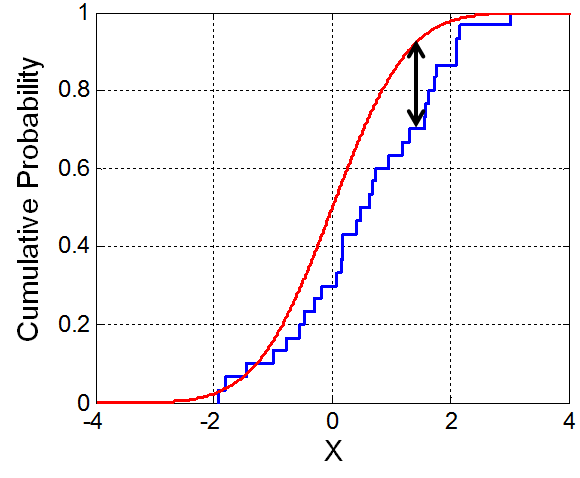
\includegraphics[width=0.45\linewidth]{figs/KS_Example.png}~~~
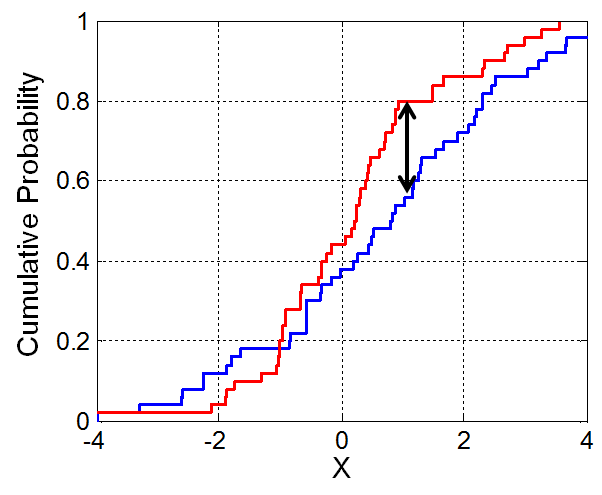
\includegraphics[width=0.45\linewidth]{figs/KS2_Example.png}
\caption{An example Kolmogorov statistic comparing an empirical CDF
with a known, exact CDF (left)  and a Kolmogorov statistic comparing
two empirical CDFs (right). The statistic is indicated by the black,
double-sided arrow. Images taken from 
Wikipedia~\cite{Wiki_kolm}.}
\label{fig:kolm}
\end{figure}

We start with some preliminary definitions. The {\it indicator function}
\index{indicator function} of a subset $A$ of a set $B$ is
the function $\id_A:B\to\{0,1\}$ given by
\begin{equation}
  \id_A(x)=\begin{cases}
    1 & \text{if } x\in A, \\
    0 & \text{otherwise}.
  \end{cases}
\end{equation}
Given some measurements $X_1,...,X_N$, we construct
the {\it empirical CDF} as
\begin{equation}\label{eq:empcdf}
  \bar{F}(x)=\frac{1}{N}\sum_{i=1}^N\id_{[X_i,\infty]}(x),
\end{equation}
where each term counts the number of data less than
or equal to $x$.
The measurements have the same CDF, so at each $x$
we have by the LLN
\begin{equation}\label{eq:empcdfconv}
  \begin{aligned}
  \bar{F}(x)\xrightarrow{\text{P}}
    \ev{\frac{1}{N}\sum_{i=1}^N\id_{[X_i,\infty]}(x)}
    &=\frac{1}{N}\sum_{i=1}^N\ev{\id_{[X_i,\infty]}(x)}\\
    &=\frac{1}{N}\sum_{i=1}^N\pr{X_i\leq x}\\
    &=\frac{1}{N}\sum_{i=1}^NF(x)\\
    &=F(x),
  \end{aligned}
\end{equation}
i.e. $\bar{F}$ is an unbiased, consistent estimator. 
%Before we compute the
%variance, we should note that the variance of each indicator is
%\begin{equation}
%  \sigma^2_\id=\ev{(\id-F)^2}
%              =\ev{\id^2+F^2-2\id F}
%              =F(1-F),
%\end{equation} 
%where we have suppressed the dependence on $x$ and the random variable
%for notational convenience, and utilized $\id^2=\id$. The variance
%of $\bar{F}$ easily follows:
%\begin{equation}
%  \variance\bar{F}(x)=\frac{1}{N^2}\sum_{i=1}^N
%                  \variance{\id_{[X_i,\infty]}(x)}
%                =\frac{1}{N}F(x)\left(1-F(x)\right).
%\end{equation}

The {\it Kolmogorov statistic} is
\begin{equation}
  \Delta\equiv\max_{x\in\R}\left|\bar{F}(x)-F(x)\right|.
\end{equation}
Since $\bar{F}(x)\xrightarrow{\text{P}}F(x)$ for all $x$, it follows
that $\Delta\xrightarrow{\text{P}}0$. An important but surprising
fact about $\Delta$ is that it is {\it distribution free}.
The proof is relatively straightforward and given in
\thmref{thm:koldf}. \thmref{thm:kolprb} gives
the probability that the difference between the empirical and true
CDFs is at least as extreme as what we calculate. This proof is
tedious and not particularly enlightening, so it has been omitted.
If you want to see a proof you can read Berg~\cite{berg_markov_2004},
who attributes it to Birnbaum and Tingey~\cite{birnbaum_one-sided_1951}
and Smirnov~\cite{smirnoff_sur_1939}.
\begin{theorem}{}{koldf}
  All continuous $F$ have the same $\Delta$. 
  \begin{proof}
    We will start with the slightly easier case where $F$ is monotonically
    increasing. In this case, $F^{-1}$ exists and is also monotonically
    increasing. Then by making the variable change $y=F(x)$ we find
    \begin{equation*}
      \begin{aligned}
      \Delta&=\max_{x\in\R}\left|\bar{F}(x)-F(x)\right|\\
            &=\max_{y\in[0,1]}\left|
                \bar{F}\left(F^{-1}(y)\right)-F\left(F^{-1}(y)\right)\right|\\
            &=\max_{y\in[0,1]}\left|
                \bar{F}\left(F^{-1}(y)\right)-y)\right|.
      \end{aligned}
    \end{equation*}
    Let's focus on the $\bar{F}(F^{-1}(y))$ term. We can recast this as
    $$
      \bar{F}\left(F^{-1}(y)\right)
          =\frac{1}{N}\sum_{i=1}^N\id_{[X_i,\infty]}\left(F^{-1}(y)\right)
          =\frac{1}{N}\sum_{i=1}^N\id_{[F(X_i),\infty]}(y),
    $$
    where in the second step we used 
    $F(X)\leq y\Leftrightarrow X\leq F^{-1}(y)$. This shows that the
    empirical CDF of $F^{-1}(y)$ is none other than the empirical CDF 
    of the sample $F(X_1),...,F(X_N)$. But
    $$
      \pr{F(X)\leq t}=\pr{X\leq F^{-1}(t)}=F\left(F^{-1}(t)\right)=t,
    $$
    i.e. the sample is drawn from the uniform distribution in the
    interval $[0,1]$, regardless of what $F$ is. It follows that 
    $\bar{F}\left(F(y)\right)$ is independent of $F$, and hence so 
    is $\Delta$.

    In the case $F$ is not monotonic, the inverse is not guaranteed.
    We define
    $$
      F^+(y)\equiv\min\{x\,|\,F(x)\geq y\}.
    $$
    The important thing is that $F^+(y)\leq z\Leftrightarrow y\leq F(z)$.
    To see this note that
    $$
      F^+(y)\leq z \Rightarrow y\leq F\left(F^+(y)\right)\leq F(z)
    $$
    and
    $$
      y\leq F(z)\Rightarrow F^+(y)\leq F^+\left(F(z)\right)\leq z.
    $$
    The theorem follows by replacing $F^{-1}$ with $F^+$ 
    in the first paragraph.
  \end{proof}
\end{theorem}
\begin{theorem}{}{kolprb}
  Let $D>0$. Then
  $$
    \pr{\Delta>D}=\sum_{k=0}^K{N\choose k}D\left(D+\frac{k}{N}\right)^{k-1}
                   \left(1-D-\frac{k}{N}\right)^{N-k},
  $$
  where $K$ is determined by the condition that $1-D-k/N$ cannot be
  negative. If $N$ is large enough, this probability can be approximated as
  $$
    \pr{\Delta>D}\approx e^{-2ND^2}.
  $$
\end{theorem}

We now have all the ingredients we need to carry out a Kolmogorov test,
and by \thmref{thm:koldf} we are guaranteed it will work, regardless
of the underlying distribution, under the modest assumption that its
CDF is continuous. In practice one can proceed as follows:
\begin{enumerate}
  \item Sort the measurements, then place them into an array $\{X_i\}$.
  \item The $X_i$ are indexed by $i$, so the corresponding empirical CDF 
        is just the array of fractions $\{i/n\}$. For example $X_1\leq X_1$, 
        so $\bar{F}(X_1)=1/N$. Since $X_1,\,X_2\leq X_2$ we have 
        $\bar{F}(X_2)=2/N$.
  \item Compute the exact PDF. For instance if we think the
        data come from $\Gau(x,0,\sigma)$, we can compute the exact CDF
        using \equatref{eq:gaussCDF}; or if we think the data come from the 
        uniform distribution on $[0,1]$, we can just heapsort them.
  \item Determine $\Delta$.
  \item Calculate $\pr{\Delta>D}$ using \thmref{thm:kolprb}.
        If the calculation of the exact probability is slow, you can
        use the approximation, but only if $N$ is big enough, say larger
        than 100 or so.
  \item The underlying assumption is that empirical CDF is an estimator
        for true CDF, so if the probability is below some threshold,
        say 0.05, then this assumption becomes suspect. 
\end{enumerate}

\section{Statistical analysis of Markov chains}
Suppose we have computed using MCMC a time series of $N$ measurements
\{$X_1$, ..., $X_N$\}. In principle each element of this sample is drawn
from a PDF with mean $\ev{X_i}=\ev{X}=\hat{x}$ and variance 
$\sigma^2=\ev{(X_i-\hat{x})^2}$, i.e. they all have the same mean
and variance. Unbiased estimators for the mean and variance are
\begin{equation}\label{eq:umv}
  \bar{X}=\frac{1}{N}\sum_{i=1}^N X_i
  ~~~~\text{and}~~~~
  \bar{\sigma}^2=\frac{1}{N-1}\sum_{i=1}^N (X_i-\bar{X})^2.
\end{equation}
The variance of the random variable $\bar{X}$ is
\begin{equation}\label{eq:tsvar}
  \sigma^2_{\bar{X}}=\ev{(\bar{X}-\hat{x})^2}
                    =\frac{1}{N^2}\left(\sum_{i\neq j}\ev{X_iX_j}
                     +N\ev{X^2}\right)-\hat{x}^2.
\end{equation}
In the case that the measurements are uncorrelated, the expected values
factorize, and we obtain
\begin{equation}
  \sigma^2_{\bar{X}}=\sigma^2/N
\end{equation}
in agreement with the CLT. But in practice measurement
$i+1$ is often correlated with measurement $i+t$ because they are from
the same time series. To measure this we draw inspiration from 
definition \eqref{dfn:cor}. 
The {\it autocovariance}\index{autocovariance} between measurements 
$X_i$ and $X_{i+t}$ is
  \begin{equation}\label{dfn:acov}
    c(X_i,X_{i+t})\equiv\ev{(X_i-\hat{x})(X_{i+t}-\hat{x})}
     =\ev{X_iX_{i+t}}-\ev{X_i}\ev{X_{i+t}},
  \end{equation}
For a Markov process in equilibrium, the autocovariance depends only on 
the separation $t$, so we define $c(t)\equiv c(X_i,X_{i+t})$. Finally note that
$c(0)=\sigma^2$, which motivates the definition of the {\it autocorrelation}
\index{autocorrelation}
\begin{equation}\label{dfn:acor}
  \gamma(t)\equiv\frac{c(t)}{\sigma^2}.
\end{equation}
The autocorrelation decays in $t$ as a sum of exponentials. I don't
know why this is true, and I couldn't find a reference, but this is what
everybody says. Assuming this is the case we can write
\begin{equation}
  \gamma(t)=A_\text{exp}\,e^{-t/\tau_\text{exp}}
            +\sum_{i=1}^\infty A_i\,e^{-t/\tau_i},
\end{equation}
where the $A$s are constants and we have picked out the leading
exponential behavior; i.e. for all $i$
\begin{equation}\index{autocorrelation time!exponential}
  \tau_\text{exp}>\tau_i.
\end{equation}
$\tau_\text{exp}$ is called the {\it exponential autocorrelation time}.

Plugging definition \eqref{dfn:acov} into \equatref{eq:tsvar} we have 
\begin{equation}
  \sigma^2_{\bar{X}}=\frac{1}{N^2}\sum_{i,j}c(X_i,X_j).
\end{equation}
In the last sum, $|i-j|=0$ occurs $N$ times, and $|i-j|=t$ occurs
$2(N-t)$ times. Note $1\leq t\leq N-1$. Therefore
\begin{equation}
  \sigma^2_{\bar{X}}=\frac{1}{N^2}
    \left(N\,c(0)+2\sum_{t=1}^{N-1}(N-t)c(t)\right).
\end{equation}
Finally we use $c(0)=\sigma^2$ to find
\begin{equation}\label{eq:IAC}
  \sigma^2_{\bar{X}}
    =\frac{\sigma^2}{N}\left(1+2\sum_{t=1}^{N-1}\left(1-\frac{t}{N}\right)
     \gamma(t)\right)
    \equiv\frac{\sigma^2}{N}\tau_\text{int}.
\end{equation}
The quantity
\begin{equation}\label{dfn:IAC}\index{autocorrelation time!integrated}
  \tauint=\left(1+2\sum_{t=1}^{N-1}\left(1-\frac{t}{N}\right)
   \gamma(t)\right)
\end{equation}
is called the {\it integrated autocorrelation time}.

From \equatref{eq:IAC} we see that $\tauint$ is just the ratio between the
estimated variance of the sample mean and what this variance would have been 
if the data were uncorrelated. 

In practice, we often don't know the true mean $\hat{x}$ of the time series.
Therefore along the lines of \equatref{eq:umv}, we construct an unbiased
estimator of the autocovariance
\begin{equation}
  \bar{c}(t)=\frac{N}{(N-1)(N-t)}
    \sum_{i=1}^{N-t}(X_i-\bar{X})(X_{i+t}-\bar{X}),
\end{equation}
where it is the factor $N/(N-1)$ that removes the bias, just as before.
Also in most situations we work in the limit where $N$ is large. In this
limit, we can construct an estimator for $\tau_\text{int}$ by
\begin{equation}\label{eq:IACest}
  \bar{\tau}_\text{int}(n)=1+2\sum_{t=1}^n\bar{\gamma}(t),
\end{equation}
where $n<N$. To understand the above estimator look at definition
\eqref{dfn:IAC}. When $t$ is small, $1-t/N\approx 1$. Large $t$ terms
are doubly suppressed by the exponential decay of $\gamma(t)$ and
by $1-t/N\approx 0$. If the estimator still makes you uncomfortable,
note that in the overly simplistic case where
$\gamma(t)$ has only one exponential term, one can prove
\begin{equation}
  \lim_{N\to\infty}\tau_\text{int}=1+2\sum_{t=1}^\infty\gamma(t),
\end{equation}
which parallels \equatref{eq:IACest} more closely. To construct a final
estimator for $\tauint$, one looks for a window in $n$ for which
\equatref{eq:IACest} becomes roughly independent of $n$. This serves
as the final $\bar{\tau}_\text{int}$.

\bibliographystyle{unsrtnat}
\bibliography{bibliography}

\chapter{Physics: Statistical Physics}\label{ch:statphys}

One regime of interest for lattice QCD calculations is the application
of lattice formalism to hot, dense nuclear systems; this is the realm
of thermodynamics\index{thermodynamics} and statistical physics. In this chapter I try to
offer some reminders of statistical physics, especially those that
are directly relevant to modern lattice investigations of the QCD
phase diagram. Some references I drew from include
Ref.~\cite{tahir-kheli_general_2012} and \cite{kardar_statistical_2007}.

\section{A brief history of early thermodynamics}

As it turns out, much of thermodynamics was discovered in order to develop
and increase the efficiency of engines. This presentation is based
on Ref.~\cite{wiki:thermo}. The first engine progenitor that I'm
aware of would be the vacuum pump, which was built and designed by Otto von 
Guericke in 1650. Shortly thereafter, Boyle and Hooke developed an air pump.
Playing around with this air pump helped reveal {\it Boyle's law}\index{Boyle's
law}
\begin{equation}
  P\propto\frac{1}{V},
\end{equation}
a relationship between the pressure $P$ and volume $V$ of a gas.

In 1697, Denis Papin developed a steam digester, a closed vessel which trapped steam 
until a high pressure was generated, with a valve to release pressure to keep it
from exploding.  He noticed the value would rhythmically move up and down and was 
inspired to create a piston and cylinder engine; however, he did not pursue this design. 
In 1712, Thomas Newcomen built the first engine based on Papin's concept.
This\index{engine!Newcomen} {\it Newcomen engine} was quite inefficient; by
1781, major improvements were made by James Watt, including making the condenser a separate
entity to avoid energy loss repeatedly cooling and re-heating the cylinder and
implementing rotary motion, allowing the\index{engine!Watt} {\it Watt engine} to 
be more broadly applicable.
Such early engines are examples of {\it external combustion engines}, which
burn\index{engine!external combustion}
fuel, using the heat to increase the temperature of some liquid whose
pressurized vapor is used to move something.

The development of thermodynamics as a modern science arguably begins with
with Sadi Carnot, who in 1824 published {\it Reflections on the Motive Power of
Fire}, a text on heat, power, energy and engine efficiency. 
His book outlined energetic relations between the\index{Carnot!engine}
Carnot engine, the\index{Carnot!cycle} Carnot cycle, and motive power. 
In 1850, Clausius published a paper titled ``On the Moving Force of Heat", which 
first stated the basic principles of the second law of thermodynamics. 
He introduced the concept of entropy\index{entropy} in 1865.

In parallel to the development of thermodynamics as a discipline was the
constant improvement of commercial engine efficiency. Of particular note for
modern transportation is the constant improvement of the {\it internal
combustion engine}\index{engine!internal combustion}, where the products of fuel
combustion themselves directly provide the pressure used to produce mechanical
motion. These improvements were due to many scientists and engineers and
happened over the course of many years~\cite{wiki:internalCE}.
A few notable engineers, which include some household names, are listed in
chronological order of their contributions:
In 1872, George Brayton invented the first commercial liquid-fueled 
internal combustion engine. In 1876, Nicolaus Otto, in cooperation with Gottlieb 
Daimler and Wilhelm Maybach, patented the four-stroke cycle engine with a 
compressed charge. Karl Benz, four years later in 1879, patented a 
dependable two-stroke gas engine. Lastly, in 1892 Rudolf Diesel\footnote{Diesel
engines tend to be more efficient for transportation 
than gas engines, in the sense that they tend
to deliver more distance per unit fuel. One of the reasons for this is that the
combustion is triggered by high pressure instead of a spark, which requires more
compression. When the gas then expands, it therefore pushes the piston a larger
distance. Diesel died under mysterious circumstances--one likely possibility is that he
was assassinated.} invented the 
first compressed charge, compression ignition engine.


\section{The laws of thermodynamics}

In thermodynamics, one usually divides the universe into a system 
(or collection of systems) under
consideration and its (their) surroundings.
The {\it zeroth law of thermodynamics} is just the statement that
equilibrium is transitive.\index{thermodynamics!zeroth law}
\begin{theorem}{Zeroth law of thermodynamics}{}
  If two systems $A$ and $B$ are in equilibrium with a system $C$, then
$A$ and $B$ are also in equilibrium.
\end{theorem}
Let $U$ be the energy of any system,
$Q$ the heat added to it, and
$W$ the work done on it. The {\it first law of thermodynamics}
is the statement of energy conservation.\index{thermodynamics!first law}
\begin{theorem}{First law of thermodynamics}{}
  $$\dd U=Q+W$$
\end{theorem}
%In other words, heat and work are the only ways to change a system's energy.

These two laws are relatively straightforward to understand. But to understand
the second law, one needs the concept of entropy. First we will proceed
using discoveries by Carnot and Clausius, which I think is valuable
because it helps one understand why $Q=T\dd S$. Then we will take a look at an
information-oriented understanding of entropy. Both of these follow the
presentations in Ref.~\cite{kardar_statistical_2007} closely.



\begin{figure}
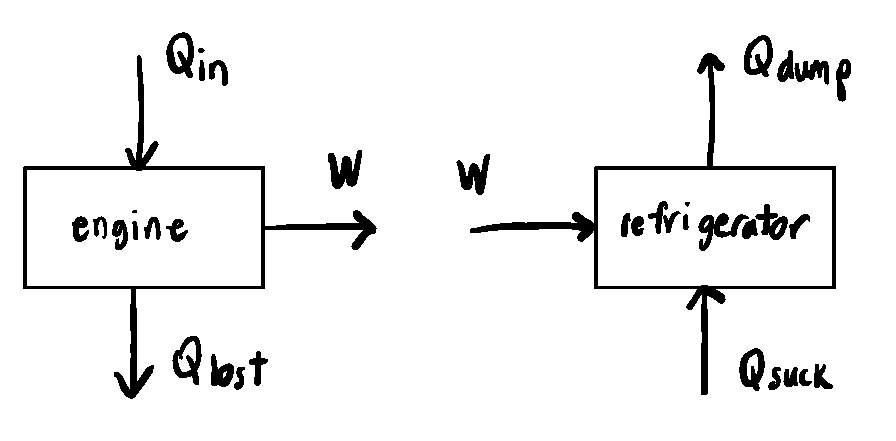
\includegraphics[width=\linewidth]{figs/engineFrige.pdf}
\caption{Schematic diagrams for an ideal engine (left) and refrigerator (right).}
\label{fig:engineFrige}
\end{figure}



\subsection{Entropy from engines}

A {\it heat engine}\index{engine!heat} is any idealized system that takes in
heat $\Qin$ from a source, converts some of that into work $W$, and loses some heat to its
surroundings $\Qlost$. A reasonable measure of its efficiency\footnote{It is not
clear to me at this stage that this is the ``best" definition of efficiency or a
unique one. In particular, one could raise this ratio of heat to an arbitrary
(positive) power. In a sense, using 1 as the power is the simplest possible definition. 
Additionally, when we derive
the Carnot engine efficiency, we will see that it related to the ratio
of two temperatures raised to some power. There also we have the freedom to
pick a power, and again the simplest decision is 1. Picking the same power for
the heat and the temperature ratios is important so that the entropy derived from
engines matches the microcanonical (or information) entropy, which we will derive
later.} is
\begin{equation}\label{eq:engineEff}
  \text{efficiency}=\frac{W}{\Qin}=\frac{\Qin-\Qlost}{\Qin}\leq1,
\end{equation}
where the inequality is due to the first law of
thermodynamics\footnote{Incidentally, this rules out any (perpetual motion)
machine that can produce more energy than you put in.}.
A {\it refrigerator}\index{refrigerator} is any idealized system that does the
opposite; i.e. it takes in some work $W$ to suck some heat $\Qsuck$ out of
some source, and dumps that heat $\Qdump$ into its environment.
Similarly, a reasonable measure of the refrigerator's efficiency is
\begin{equation}\label{eq:refrigeratorEff}
  \text{efficiency}=\frac{\Qsuck}{W}=\frac{\Qsuck}{\Qdump-\Qsuck},
\end{equation}
Schematics of an ideal engine and refrigerator are given in
\figref{fig:engineFrige}.
With this terminology, we give two equivalent statements of the second law,
which as far as I can tell, are just things that were empirically observed
when developing engines:\index{thermodynamics!second law}
\begin{enumerate}
  \item (Kelvin) There is no process whose sole result is the conversion of heat
        into work. In other words the inequality in \equatref{eq:engineEff}
        should be strict.
  \item (Clausius) There is no process whose sole result is the transfer of
        heat from a colder system to a warmer one. In other words, the
        efficiency \eqref{eq:refrigeratorEff} is finite.
\end{enumerate}
It is not too difficult to show using ideal engines and refrigerators
that these two formulations are equivalent~\cite{kardar_statistical_2007}.
Later, we will formulate these in terms of a new quantity, entropy. The
formulation in terms of entropy can be proven in the framework of statistical
physics.

In order to examine systems in detail, we need to be in equilibrium so that all
thermodynamic coordinates are well defined.
If nothing changes, a system remains in equilibrium; it stands to reason that
if a process happens sufficiently slowly, it is more or less still in
equilibrium. Such processes are called\index{quasistatic} {\it quasistatic}.
A process is {\it adiabatic}\index{adiabatic} if $Q=0$ throughout that process.

Next we introduce the idea of a\index{engine!Carnot} {\it Carnot engine},
which should theoretically be the most efficient engine possible. 
It turns out that the most important property of such an engine is that it 
is\index{reversible} {\it reversible}, i.e. that you can reverse all its inputs
and outputs with the result that it works like the forward engine running
backwards in time. In particular a Carnot engine is reversible,
runs\index{cycle} in a {\it cycle}, i.e. it returns to its original state
at the end of its process, and its heat exchanges occur at 
temperatures\footnote{A Carnot cycle generically consists of two adiabats
and two isotherms. Specifying the heat exchanges at these temperatures allows us
to pick two isotherms. One can theoretically find adiabats using, e.g. an ideal
gas, but in principle Carnot engines with other materials are possible.}
$T_H$ and $T_C$, i.e. it draws and dumps heat without changing the
temperatures of its surroundings.
Looking at \figref{fig:engineFrige}, we see that a Carnot
engine run backward in time is just a Carnot refrigerator, and vice versa.

\begin{figure}
\centering
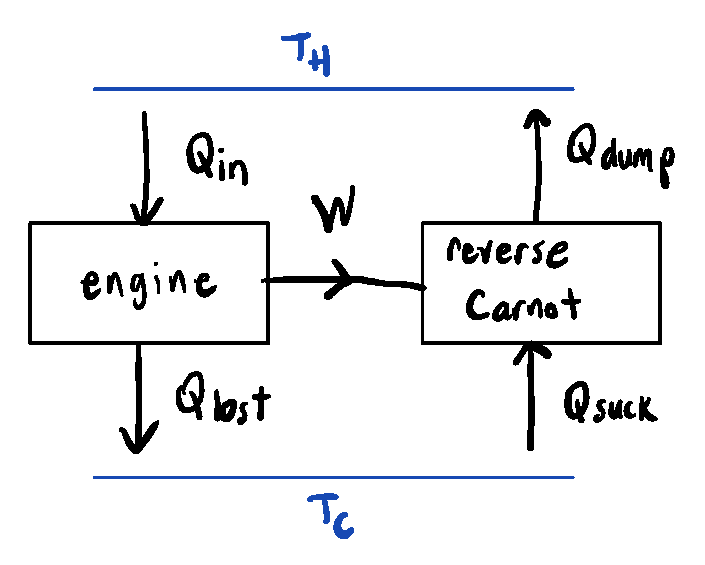
\includegraphics[width=0.7\linewidth]{figs/carnotThm.pdf}
\caption{An idealized machine used to prove Carnot's theorem.}
\label{fig:carnot}
\end{figure}

To see why this reversibility matters, consider \figref{fig:carnot}. In this
system, we use any engine to draw heat from a hot reservoir fixed at
$T_H$ that loses heat to a cold reservoir $T_C$ with $T_H>T_C$. We reverse a Carnot engine,
and use the output work from the left engine as input work to the reversed
Carnot engine. This combined system works as a process whose sole result 
transfers heat between the top and bottom reservoirs. By Clausius's statement 
of the second law of thermodynamics, it must be that $\Qin\geq\Qdump$ and
$\Qlost\geq\Qsuck$. It follows that
\begin{equation}
\text{efficiency}=\frac{W}{\Qin}\leq\frac{W}{\Qdump}=\text{Carnot engine
efficiency}.
\end{equation}

\index{Carnot's theorem}
\begin{theorem}{Carnot}{}
No engine is more efficient than a Carnot engine.
\end{theorem}

\begin{corollary}{Carnot}{carnot}
All Carnot engines have the same efficiency $\eta(T_H,T_C).$
\end{corollary}

\begin{figure}
\centering
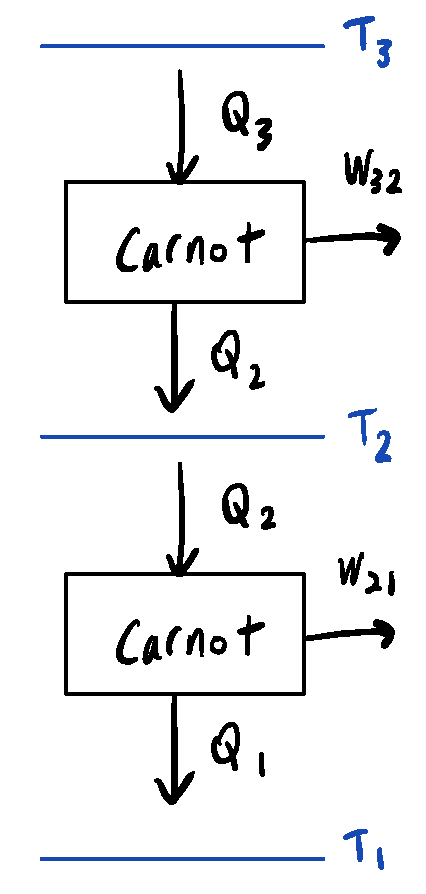
\includegraphics[width=0.6\linewidth]{figs/carnotSeries.pdf}
\caption{A series of Carnot engines.}
\label{fig:carnotSeries}
\end{figure}

Next, we are going to derive a relationship between heat flow and reservoir
temperature for the Carnot engine. Once we have this relationship, we will
creatively apply our knowledge of Carnot engines to say something about heat
flow and temperature generally. This will ultimately lead us to conclude that
entropy exists, and deliver a definition of it.

To derive the aforementioned relationship, consider a series of Carnot engines
as shown\footnote{The Carnot engines are identical and reversible, so it
must be that the heat exchanges on either side of $T_2$ are the same.}
in \figref{fig:carnotSeries} with $T_3>T_2>T_1$. The total effect of this
Carnot series is to take in heat $Q_3$, lose heat $Q_1$, and do work
$W_{31}=W_{32}+W_{21}.$ Using \corref{cor:carnot} 
we find that the heat exchanges must be related by
\begin{equation}\begin{aligned}
  Q_2 &= Q_3 - W_{32} &&= Q_3\left(1-\eta(T_3,T_2)\right) \\
  Q_1 &= Q_2 - W_{21} &&= Q_2\left(1-\eta(T_2,T_1)\right) 
                  = Q_3\left(1-\eta(T_3,T_2)\right)\left(1-\eta(T_2,T_1)\right) \\
  Q_1 &= Q_3 - W_{31} &&= Q_3\left(1-\eta(T_3,T_1)\right).
\end{aligned}\end{equation}
From the last two equations, it follows
\begin{equation}
\left(1-\eta(T_3,T_2)\right)\left(1-\eta(T_2,T_1)\right) =
1-\eta(T_3,T_1).
\end{equation}
Whatever the functional form of $1-\eta$ is, the middle temperature must be
cancelled through a multiplication. Hence $1-\eta$ must be a ratio of its input
temperatures, raised to some power. The simplest choice\footnote{Again, this
choice also will help our definition of entropy match that from the
microcanonical ensemble.} that guarantees $0\leq\eta<1$ is
\begin{equation}\label{eq:carnotEfficiency}
  \frac{Q_1}{Q_2}=1-\eta(T_2,T_1)\equiv\frac{T_1}{T_2}.
\end{equation}

It is nice to have this expression for the Carnot engine efficiency.
But again, from my perspective, it's more interesting to have this relation between
heat and temperature at the input and output heat vents for the engine.
Indeed, we can now potentially learn something about heat delivered
to an arbitrary system at some temperature, and we will leverage this trick to
prove a theorem due to Clausius.

\begin{figure}
\centering
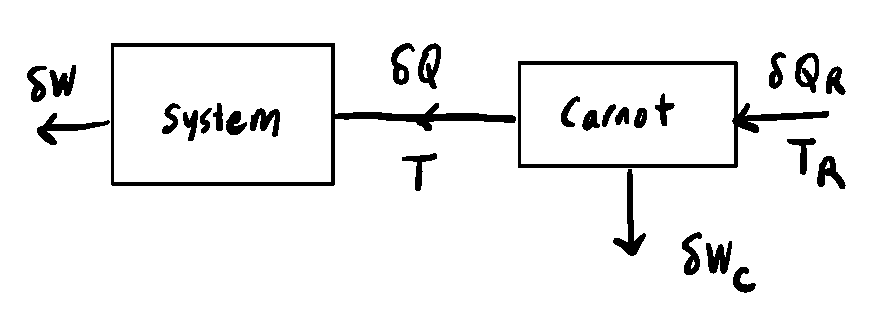
\includegraphics[width=\linewidth]{figs/clausius.pdf}
\caption{A convenient setup used to prove Clausius's theorem.}
\label{fig:clausius}
\end{figure}

\index{Clausius's theorem}
\begin{theorem}{Clausius}{}
For any cyclic transformation,
$$ \oint\frac{\delta Q}{T}\leq0. $$
where $\delta Q$ is a small amount of heat supplied at temperature $T$ to
a system during part of the cycle.
\begin{proof}
Consider the setup of \figref{fig:clausius}. The directions of heat and
work can be chosen as given WLOG. We begin with a system that
has a small amount of heat $\delta Q$ delivered to it at temperature $T$; by
energy conservation, some work $\delta W$ will leave the system.
To leverage \equatref{eq:carnotEfficiency}, we direct $\delta Q$ to the output port
of a Carnot engine, which generically takes in heat $\delta Q_R$ from a
reservoir at temperature $T_R$ and does some work $\delta W_E$.
From \equatref{eq:carnotEfficiency} we have
\begin{equation*}
\delta Q_R=T_R\frac{\delta Q}{T}.
\end{equation*}
After returning to their original states, the system and Carnot engine have the
combined effect of taking in heat $Q_R=\oint\delta Q_R$ and doing work $W$.
By energy conservation $Q_R=W$. By Kelvin's statement of the second law, it must
be that positive work is done on the system and positive heat leaves
the system; given our arrow conventions, we conclude $W=Q_R\leq0$. Hence
\begin{equation*}
T_R\oint\frac{\delta Q}{T}\leq0.
\end{equation*}
That $T_R$ is non-negative proves the theorem.
\end{proof}
\end{theorem}

We are finally in a position to define\index{entropy} entropy.
In particular, if we further specify that the cycle is reversible,
we will find that $\delta Q\to-\delta Q$ when we switch the direction of the
cycle. It follows that for a reversible cycle
\begin{equation}
 \oint\frac{\delta Q}{T}=0. 
\end{equation}
This tells us that the process is path-independent, which means we can define a
new function $S$ with
\begin{equation}
 S(B)-S(A)=\int_A^B\frac{\delta Q}{T}. 
\end{equation}
Hence we learn for reversible\footnote{I've seen examples of people defining
reversible\index{reversible} systems to be those that have $Q=T\dd S$.}, 
quasistatic\footnote{Lattice calculations are always done under the assumption
of equilibrium, which means it's quasistatic by definition.} changes
\begin{equation}
Q=T\dd S.
\end{equation}
It follows that reversible, adiabatic processes are\index{isentropic} isentropic.
We also get this statement of the first law:\index{thermodynamics!first law}
\begin{equation}
 \dd U = T\dd S+P\dd V.
\end{equation} 

Finally, consider a possibly irreversible path from $A$ to $B$ that is closed
with a reversible one from $B$ to $A$. From Clausius's theorem, we get
\begin{equation}
\int_A^B\frac{\delta Q}{T}+\int_B^A\delta Q_{\text{rev}}\leq0
\end{equation}
or
\begin{equation}
\int_A^B\frac{\delta Q}{T}\leq S(B)-S(A).
\end{equation}
It follows that $\delta S\geq\delta Q/T$ for any process. In particular consider
two systems that are originally isolated from each other and separately in
equilibrium, then allow them to exchange heat. Since there is no work, we must
have $\delta Q_{\text{total}}=0$ by the first law, and hence $\delta
S_{\text{total}}\geq0$. This is the more familiar statement of
the {\it second law of thermodynamics}.\index{thermodynamics!second law}
\begin{theorem}{Second law of thermodynamics}{}
If two or more adiabatically isolated systems are brought into thermal contact,
their combined entropy must always increase.
\end{theorem}

In the context of statistical physics, this statement will follow from
probabilistic considerations. There we will see that systems in equilibrium have
maximum entropy. What about statements of minimum entropy? This is covered by
the {\it third law of thermodynamics}, which is an observation.\index{thermodynamics!third law}
\begin{theorem}{Third law of thermodynamics}{}
$$
  \lim_{T\to0}S(T)=0
$$
\end{theorem}


\subsection{Entropy from information}

\section{Equations of state}\label{sec:EoS}


Probably the equation of state that you are most familiar with is the 
ideal gas law,\index{ideal gas law}
\begin{equation}
  PV=NkT.
\end{equation}
The volume $V$ and the number of particles $N$ both scale linearly with the
size of the system; we call such variables {\it extensive}\index{extensive}. 
Meanwhile the pressure $P$ and the temperature $T$ are {\it intensive}\index{intensive}, 
i.e. they do not scale with the system.

There is an equation of state for each intensive variable required for the
description of thermodynamic states. For example from the
first law of thermodynamics,\index{thermodynamics!first law}
\begin{equation}\label{eq:fslaw}
  \dd{U}=T\dd{S}-P\dd{V}+\sum_i\mu_i\dd{N}_i,
\end{equation}
we know that\footnote{It can be quite confusing to track which variables
are held fixed and allowed to vary doing these partial derivatives.
This matters because sometimes different choices of control parameters
are related to each other through a constraint.
You can get a hint for example by looking at equations like
\equatref{eq:fslaw}, which is a reminder we are thinking of
$U$ as a function of the set \{$S$, $V$, $\vec{N}$\}. In this context,
partial derivatives with respect to one of those variables must
guarantee the others in that set are fixed.}

\begin{equation}
  T=\pdv{U}{S}.
\end{equation}
This intensive variable $T$ depends on only the extensive variables; 
generally we could write
\begin{equation}
  T=T(U,S,V,N).
\end{equation}
This is what we call an {\it equation of state}\index{equation of state}
(EoS). The arguments are sometimes referred to as 
{\it control parameters}\index{control parameter}. Knowing every equation 
of state is enough to reconstruct the fundamental equation, and therefore 
enough to determine the physics of the system.

\section{Legendre transforms}\index{Legendre transformation}

Equation~\eqref{eq:fslaw} tells us that we can think of the internal energy
$U$ of a system in equilibrium at $(T,P,\mu)$ as a function of $S$, $V$, and
$N$. However one of the control parameters, such as $S$, may be
difficult or impossible to measure, and therefore we would rather
think in terms of the more accessible quantity $T$, which 
is the derivative of $U$ with respect to $S$; 
Hence we want 
\begin{enumerate}
\item to look at $U$ in terms of a derivative with respect to $S$ rather 
      than $S$ itself; moreover 
\item we don't want to lose any information we had before, i.e. we want this
      process to be invertible. 
\end{enumerate}
These are the purposes of a Legendre transformation. The second point 
may seem too obvious to state, but it's worth emphasizing here because 
what makes thermodynamic potentials such as $U$ special is that you're 
supposed to be able to determine state variables like $T$ from them. 
Since no information is lost, Legendre transforms guarantee that 
thermodynamic potentials get transformed to other thermodynamic potentials.
\index{thermodynamic!potential}\index{potential!thermodynamic}

Before we define a Legendre transformation, let's look at an example
due to Markus Deserno~\cite{deserno} where a naive transformation can go
wrong and information can be lost. 
\begin{example*}{}
We consider a function $y(x)$ and define a new variable
\begin{equation}\label{eq:xlegendre}
  p\equiv y'(x).
\end{equation}
In order to accomplish goal (1) above, one might naively solve
\equatref{eq:xlegendre} for $x$, obtaining the function $x(p)$
and then plug this back into $y(x)$ to obtain
\begin{equation}
  Y(p)=y\left(y'^{-1}(p)\right).
\end{equation}
To see that this procedure destroys information, consider the example
\begin{equation}\label{eq:badlegendre}
  y(x)=\frac{1}{2}(x-x_0)^2.
\end{equation}
The derivative is $p=y'(x)=x-x_0$, and hence $x=p+x_0$. Plugging this
into \equatref{eq:badlegendre} we get the function
\begin{equation}
  Y(p)=y(x(p))=\frac{1}{2}\left(x(p)-x_0\right)^2=\frac{1}{2}p^2.
\end{equation}
Evidently all functions of the form~\eqref{eq:badlegendre} get transformed
to the same function regardless of the value of $x_0$; therefore there is
no way starting from $Y(p)$ to figure out what $x_0$ was. Hence
information was destroyed.
\end{example*}

Now on to the definition. Recall that a function $f$ is {\it convex}
\index{function!convex} in a region if the graph of the function lies 
below the line segment connecting any two points in that region. It is 
{\it concave}\index{function!concave} if $-f$ is convex. Consider
a function $y:\R\to\R$. Then the 
{\it Legendre transform} is defined by
\begin{equation}
Y(p)=\begin{cases}
  \min_x [y(x)-xp] & \text{if $y$ is convex}\\
  \max_x [y(x)-xp] & \text{if $y$ is concave.}
\end{cases}
\end{equation}
This definition makes sense in view of goal (1) at the beginning of this
section, assuming $y$ is differentiable. To see this, note that the maximum
or the minimum corresponds to a critical point, and so
\begin{equation}\label{eq:legendremin}
  0=\frac{d}{dx}\left[y(x)-xp\right]=y'(x)-p.
\end{equation}

We now state two useful facts about Legendre transforms. These can
be relatively straightforwardly proven. We emphasize that Legendre
transformations are only defined for concave or convex functions, and
that the concavity or convexity is important to prove the second point,
because it guarantees that the derivative is monotonic.
\begin{proposition}{}{}
  \begin{enumerate}
    \item The Legendre transformation of a convex function is concave
          and vice versa.
    \item The Legendre transformation is its own inverse.
  \end{enumerate}
\end{proposition}

Now that we have some intuition for why one might want to do a
Legendre transform, we are going to see how some other useful
thermodynamic potentials arise from carrying them out.

\subsection{Helmholtz free energy}
\index{free energy!Helmholtz}
Let us now return to our issue of dropping $S$ in favor
of $T$. According to the above section if we
Legendre transform $U(S)$ out of the variable $S$, then the minimization
will guarantee that the new independent variable is $T$. Calling
this new function $F$, we obtain
\begin{equation}\label{eq:helmholtz}
  F(V,T,N)=U-TS.
\end{equation}
This new function is guaranteed to be a thermodynamic potential, and
we give it a special name: the {\it Helmholtz free energy}.
From \equatref{eq:helmholtz} and the first law, we get
\begin{equation}\label{eq:helmholtz1st}
  \dd F = -P\dd V -S\dd T +\sum_i\mu_i\dd{N}_i.
\end{equation}

We can derive some useful thermodynamic relations from these. For
instance
\begin{equation}\label{eq:dfdt}
  -T^2\pdv{(F/T)}{T}=U=\pdv{(\beta F)}{\beta},
\end{equation}
where $\beta=1/T$ in natural units.


\subsection{Enthalpy}\index{enthalpy}

The {\it enthalpy} is given by the Legendre transformation
\begin{equation}\label{eq:enthalpy}
 H(S,P,N)=U+PV.
\end{equation}
From \equatref{eq:enthalpy} and the first law we obtain
\begin{equation}
 \dd H = T\dd S +V\dd P +\sum_i\mu_i\dd N_i.
\end{equation}


\section{Ideal quantum gas}

\subsection{Canonical formulation}

\index{gas!bose}\index{gas!fermi}
\begin{equation}
\eta=
  \begin{cases}
     +1 & \text{bosonic gas} \\
     -1 & \text{fermionic gas}.
  \end{cases}
\end{equation}

\subsection{Grand canonical formulation}

% keep discussion general to mu_i N_i
\index{fugacity}
\begin{equation}\label{eq:fugacity}
  z=e^{-N\mu/T}
\end{equation}

The {\it grand potential} is\index{grand potential}
\begin{equation}\label{eq:grand}
  \Phi\left(V,T,\vec{\mu}\right)=U-TS-\sum_i\mu_i N_i=-T\log\grandZ
\end{equation}
from which one gets
\begin{equation}\label{eq:1stlawgrand}
  \dd\Phi=-P\dd V-S\dd T-\sum_i N_i\dd\mu_i.
\end{equation}
Since $\log\grandZ$ is extensive, it must be that
\begin{equation}
-T\log\grandZ=kV
\end{equation}
for some intensive $k$. Hence\footnote{Sometimes it is convenient to work
with $\muh\equiv\mu/T$ and $T$ instead of $\mu$ and $T$. This equation
holds for both sets of control variables since both $\mu$ and $T$ are
held fixed.} from \equatref{eq:1stlawgrand}
\begin{equation}
P=-\pdv{\Phi}{V}=-k,
\end{equation}
which means we can identify
\begin{equation}\label{eq:pgrand}
P=\frac{T}{V}\log\grandZ.
\end{equation}

Reorganizing \equatref{eq:grand} using \equatref{eq:pgrand}
yields the {\it Gibbs-Duhem relation}
\index{Gibbs-Duhem relation}
\begin{equation}
  s=\frac{\epsilon}{T}+\frac{P}{T}-\sum_i\frac{\mu_i}{T}n_i,
\end{equation}
where $s\equiv S/V$ is the entropy density, and $\epsilon$ and $n_i$
are the energy and number densities.
Taking a derivative of \equatref{eq:pgrand} w.r.t. $\mu_i$ and
using \equatref{eq:1stlawgrand} yields
another often useful relation,
\begin{equation}
  \frac{N_i}{V}=\pdv{P}{\mu_i}.
\end{equation}

\section{Relativistic quantum gases}

Relativistic quantum gases are especially interesting for us
to consider because of their
application to low temperatures of the QCD phase diagram. There, the medium
behaves approximately like a relativistic gas of hadronic bound states.
This allows for a cross check against lattice QCD at low temperatures
and at finite densities. Following some lecture notes by F. Karsch,
we are going to derive the
pressure. From this we can derive other thermodynamic quantities
using standard thermodynamic relations.

We use units $\hbar=c=k_B=1$ and consider a gas of a single species
with spin $s$ and rest mass $m$. Working in the rest frame of the gas,
we have
\begin{equation}\label{eq:dispersion}
  E=\sqrt{p^2+m^2}.  
\end{equation}
From the grand canonical formulation,
doing the momentum integral in spherical coordinates, the pressure is
\begin{equation}
  \frac{P}{T}=-\frac{4\pi\eta g}{(2\pi)^3}\int_0^\infty 
      \dd{p}p^2\log\left(1-\eta z e^{-E/T}\right),
\end{equation}
where $g=2s+1$ is the {\it degeneracy factor}. \index{degeneracy factor}
Solving the dispersion relation
for $p$ and substituting it into the pressure gives
\begin{equation}
  \frac{P}{T}=-\frac{4\pi\eta g}{(2\pi)^3}\int_m^\infty 
      \dd{E}E\left(E^2-m^2\right)^{1/2}\log\left(1-\eta z e^{-E/T}\right).
\end{equation}
Expanding the logarithm yields
\begin{equation}\label{eq:pressE}
  \frac{P}{T}=\frac{4\pi g}{(2\pi)^3}\sum_{k=1}^\infty\eta^{k+1}\frac{z^k}{k}\int_m^\infty 
      \dd{E}E\left(E^2-m^2\right)^{1/2}e^{-kE/T},
\end{equation}
which is of course only valid for $\eta z\exp(-E/T)<1$.

Let us now evaluate the integral in \equatref{eq:pressE}. We introduce
$x\equiv E/m$. Performing this variable change and integrating by parts gives
\begin{equation}\label{eq:pressint}
  \int_m^\infty\dd{E}E\left(E^2-m^2\right)^{1/2}e^{-kE/T}
  =\frac{km^4}{3T}\int_1^\infty\dd x\left(x^2-1\right)^{3/2}e^{-mkx/T}.
\end{equation}
This integral can now be expressed in terms of the
{\it modified Bessel functions}\index{Bessel function!modified}
\begin{equation}
  K_\nu(a)=\frac{\pi^{1/2}(a/2)^\nu}{\Gamma(\nu+1/2)}
             \int_1^\infty\dd x(x^2-1)^{\nu-1/2}e^{-ax}.
\end{equation}
In particular we see upon comparison with \equatref{eq:pressint}
that our integral contains $K_2(mk/T)$. Combining everything,
using $\Gamma(5/2)=3\pi^{1/2}/4$, we obtain
\begin{equation}\label{eq:pressrelQM}
  \frac{P}{T}=\frac{m^2gT}{2\pi^2}\sum_{k=1}^\infty\frac{\eta^{k+1}z^k}{k^2}
                         K_2\left(\frac{mk}{T}\right),
\end{equation}
which is a form that is well suited for computer calculations\footnote{What
one does is keep some number of terms of the above sum, usually depending
on the mass $m$; in particular $K_2$ falls off sharply for large $m$.
For very large $m$, one may choose to keep only the $k=1$ contribution,
which is the\index{Boltzmann approximation} {\it Boltzmann approximation}.}.

Other thermodynamic quantities can be derived straightforwardly
from the pressure in this form. In this context it is useful to know
the following relation for derivatives of modified Bessel functions:
\begin{equation}
  \pdv{K_\nu(z)}{z}=-K_{\nu-1}(z)-\frac{\nu}{z}K_\nu(z).
\end{equation}
Using~\equatref{eq:dfdt} one then gets for the energy density
\begin{equation}\label{eq:edensityQM}
  \epsilon=\frac{m^2gT}{2\pi^2}\sum_{k=1}^\infty\frac{\eta^{k+1}z^k}{k^2}
              \left( mk K_1\left(\frac{mk}{T}\right) 
                    + 3TK_2\left(\frac{mk}{T}\right) \right).
\end{equation}

In the context of lattice calculations, which we will discuss in more
detail in \chref{ch:realPhys}, it is often more convenient to switch
from the variable $\mu$ to $\muh\equiv\mu/T$. Besides the fact that
all quantities directly going into and coming out of lattice calculations
must be unitless, this also has the advantage of making the
fugacity blind to partial derivatives w.r.t. $T$, which are then 
interpreted as being done at fixed $\muh$.

\subsection{Hadron resonance gas}\label{sec:HRG}\index{gas!hadron resonance}

Knowing the pressure \equatref{eq:pressrelQM}, we are now ready to write down
some expressions for the {\it hadron resonance gas} (HRG) model,
following Ref.~\cite{karsch_probing_2011}. This model is interesting for lattice
results to compare against below $\Tpc$. 

The HRG model is a low-temperature model, in the sense we imagine we are working
in a phase where quarks are confined, so that the only degrees of freedom are
hadronic bound states. To a good approximation, this means we need only include
stable mesons, baryons, and their antiparticles.

\subsection{Ideal Fermi gas}\label{sec:fermi}\index{gas!ideal Fermi}

At high temperatures $T\gg\Tpc$, all the hadrons are melted, and the system is
asymptotically free. Therefore a reasonable model is of a gas of non-interacting
quarks and anti-quarks. This can also be obtained from \equatref{eq:pressrelQM}
by setting $\eta=+1$. For a single species of quark, one adds together
contributions in the integrand for both particles and antiparticles.
After performing an integration by parts, you get a simple expression for the
pressure~\cite{hegde_lattice_2008}. 
This can be used to compare against lattice results at high $T$.

\section{Bulk properties of matter}

One of the experimental goals of statistical physics is to predict some
properties of thermodynamic systems. Historically one considered e.g.
the air, which is a gas of particles. In these research notes, the focus
is rather on the bulk thermodynamics of strongly interacting matter.
A commonly used procedure is to calculate the pressure, giving
you the EoS, and to derive other thermodynamic quantities from that.
In this section we will discuss some of these quantities.

\subsection{Pressure and expansion}
The {\it speed of sound}\index{speed of sound} at fixed control parameter $X$
is given by
\begin{equation}
  c_X^2=\atFixed{\pdv{P}{\epsilon}}{X}.
\end{equation}
This is not the only expression one might encounter for a sound speed.
Qualitatively, the speed of sound should capture something like
\begin{equation}
  c_X^2=\frac{{\rm elasticity}}{{\rm inertia}}.
\end{equation}
If a material is quick to return to its original shape after deformation, a sound
wave in the material, which is caused by these kinds of movements, will have a
higher speed. Conversely if it's harder to move the constituents of the
material, i.e. if it has a higher inertia, sound speed will decrease.


The {\it compressibility}\index{compressibility} at fixed $X$ is
\begin{equation}
  \kappa_X=-\frac{1}{V}\atFixed{\pdv{V}{P}}{X},
\end{equation}
which captures how much the volume changes under a change of pressure.
Substances that take a lot of pressure to change the volume are not
very compressible; hence the minus sign.

The {\it thermal expansion coefficient}\index{thermal expansion coefficient}
at fixed $X$ is
\begin{equation}
  \alpha_X=\frac{1}{V}\atFixed{\pdv{V}{T}}{X}.
\end{equation}

\subsection{Heat storage}

The {\it specific heat} at constant volume\index{specific heat} is
\begin{equation}
  C_V=\atFixed{\pdv{U}{T}}{V}
\end{equation}
while the specific heat at constant pressure is
\begin{equation}
  C_P=\atFixed{\pdv{H}{T}}{P}
\end{equation}

\subsection{Relationships}

\begin{equation}
 \frac{\kappa_T}{\kappa_S}=\frac{C_P}{C_V}
\end{equation}
\begin{equation}
 \kappa_S=\kappa_T-\frac{\alpha_V^2 T}{n C_P}
\end{equation}


\bibliographystyle{unsrtnat}
\bibliography{bibliography}

\chapter{Physics: Renormalization Group}

These research notes were made from the perspective of a researcher working
in lattice field theory, and one advantage of the lattice, which will be
discussed later in \chref{ch:preliminaries}, is that it allows one
to make direct analogies with statistical mechanical systems, and in
particular, to utilize powerful techniques like renormalization group (RG)
analysis.

This chapter will generally try to follow 
lectures by F. Karsch, as well as the book by Binney et
al.~\cite{binney_theory_1992}, but I will also use details from a nice
book I found Bauerschmidt et al.~\cite{Bauerschmidt_2019}.
In that book, they give a nice overview of the idea
behind RG transformations, saying
\begin{quote}
Two paramount features of critical phenomena are scale invariance and 
universality. The renormalization group method exploits the scale 
invariance to explain universality. This is done via a multi-scale analysis, 
in which a system studied at a particular scale is represented by an 
effective Hamiltonian. Scales are analyzed sequentially, leading to a map 
that takes the Hamiltonian at one scale to a Hamiltonian at the next scale. 
Advancing the scale gives rise to a dynamical system defined by this map. 
Scale invariance occurs at a fixed point of the map, and different fixed
points correspond to different universality classes. The analysis of the 
dynamical system at and near the fixed point provides a means to compute 
universal quantities such as critical exponents. 
\end{quote} 
\clearpage
The goal of this chapter is to try to understand this quote in more detail,
and to learn how to carry out and interpret RG calculations that often
appear in the context of lattice field theory.

\section{Spin systems}

\section{Scaling laws}
All critical exponents\index{critical exponent} can be written as functions 
of the number of dimensions $d$ as well as $\nu$ and $\eta$. Given the reduced 
temperature\index{temperature!reduced}
\begin{equation}
  t\equiv\frac{T-T_c}{T_c}
\end{equation}
and external magnetic field $h$ one gets the 
relationships~\tabref{tab:scaling}.
These are equivalent to the {\it hyperscaling relations}
\index{hyperscaling relation}
\begin{equation}\begin{aligned}
2\beta+\gamma&=2-\alpha,\\
2\beta\delta-\gamma&=2-\alpha,\\
\gamma&=\nu(2-\eta),\\
\nu d&=2-\alpha.
\end{aligned}\end{equation}
These can be derived from the {\it scaling hypothesis}\index{scaling
hypothesis}, which we will now show for a large class of RG transformations.
\begin{table}
\begin{tabularx}{\linewidth}{lCr} \hline\hline
       Exponent & Definition & Value\\[3pt]\hline
$\alpha$ & $C_V\sim|t|^{-\alpha}$  & $2-\nu d$\\[3pt] 
$\beta$ & $m\sim|t|^{\beta}$ & $\frac{1}{2}\nu(d+\eta-2)$\\[3pt]
$\gamma$ & $\chi\sim|t|^{-\gamma}$  & $\nu(2-\eta)$\\[3pt] 
$\delta$ & $m\sim h^{1/\delta}$ &  $\frac{d+2-\eta}{d-2+\eta}$\\[3pt]
$\nu$ & $\xi\sim |t|^{-\nu}$ & \\[3pt]
        \hline\hline
\end{tabularx}
\caption{Relationships among the critical exponents. Table adapted from 
         from Ref.~\cite{binney_theory_1992}. In each case one coupling is
         small while the other is fixed to zero. For $\beta$, $t$ approaches
         zero from below.}
\label{tab:scaling}
\end{table}

Suppose we start with a system of variables $\set{\sigma}$ with Hamiltonian $H$
and $n$ couplings $\vec{k}=(k_1,...,k_n)^t$. After one RG step, we obtain
a new system of spins $\set{\sigma'}$ with $H'$ and $\vec{k}'$. We want
that expectation values remain unchanged after an RG step.
Thinking about block transformations in particular, one can
achieve this by collecting 
all those original configurations $\set{\sigma}$ that lead to the same
renormalized configuration $\set{\sigma}$\footnote{For example in the 2$d$
Ising model, if one blocks three up-spins and one down spin, there are 
four possible ways to get the same effective spin via majority rule.}, which can be
summarized as
\begin{equation}
  e^{-H'\left(\set{\sigma'},~\vec{k}'\right)}
     =e^{-\beta G(\vec{k})}\sum_{\set{\sigma}~
                        {\rm giving}~\set{\sigma'}}
      e^{-H\left(\set{\sigma},~\vec{k}\right)}.
\end{equation}
Here we have expressed an overall normalization as $e^{-\beta G}$, which will
be convenient later. When we sum over all $\set{\sigma'}$ we then get
\begin{equation}
  Z'(\vec{k}')=e^{-\beta G(\vec{k})} Z(\vec{k}),
\end{equation}
or in terms of free energies,
\begin{equation}
  F'(\vec{k}')=F(\vec{k})-G(\vec{k}).
\end{equation}
Now $F$ is extensive, so we can write
\begin{equation}
  F(\vec{k})=Nf(\vec{k})
\end{equation}
where $N$ is the number of spins on the original lattice and $f$ is intensive.
Similarly one can write
\begin{equation}
  F'(\vec{k}')=\frac{N}{b^d}f(\vec{k}')~~~~\text{and}~~~~G(\vec{k})=Ng(\vec{k}),
\end{equation}
where $b$ is the {\it scale factor}\index{scale factor}, which represents the
factor by which the lattice spacing changes. That $F$ and $F'$ are proportional
to the same intensive function with different couplings follows from the fact
that the effective Hamiltonian $H'$ has the same functional form as $H$.
Hence
\begin{equation}\label{eq:widom1}
f(\vec{k}')=b^d\left(f(\vec{k})-g(\vec{k})\right).
\end{equation}


Next, let's think about how to relate the couplings $\vec{k}'$ and $\vec{k}$
near the fixed point $\vec{k}_0$. 
We can Taylor expand $\vec{R}$ in the vicinity of $\vec{k}_0$ to find
\begin{equation}
  \vec{k}_0+\delta\vec{k}'=\vec{R}\left(\vec{k}_0+\delta\vec{k}\right)
                          \approx\vec{R}(\vec{k}_0)
                           +\frac{\partial R_i(\vec{k})}{\partial k_j}
                              \Big|_{\vec{k}=\vec{k}_0}\delta\vec{k}.
\end{equation}
The first-order term defines a matrix $M$.
Since the effect of the renormalization action
$\vec{R}$ on the fixed point is $\vec{R}(\vec{k}_0)=\vec{k}_0$, we can write
\begin{equation}
  \delta\vec{k}'=M\delta\vec{k}.
\end{equation}
Now let's switch to a basis in which $M$ is diagonal. In this basis, our
original system contains new couplings $\vec{x}$, and hence the renormalized
couplings $\vec{x}'$ are given according to the eigenvalues of $M$ as
\begin{equation}
  x_i'=\lambda_i x_i~~~~\text{no summation}.
\end{equation}
Hence we can recast eq.~\eqref{eq:widom1} as
\begin{equation}\label{eq:widom1}
f(\lambda_1x_1,\lambda_2x_2,...)=b^d\left(f(x_1,x_2,...)-g(x_1,x_2,...)\right).
\end{equation}


Now $f$ and $g$ are some kinds of functions of $\vec{x}$. Generally speaking
there will be some part that is expressible as a Taylor series in the $\vec{x}$;
this is called the {\it regular} part.\index{regular} There must also be some
part not expressible as a Taylor series in order that we can obtain the power
law behavior one finds in the vicinity of a phase transition; this is
called the {\it singular} part.\index{singular} In order to proceed we make
the following assumption: The singular part is completely contained in
$f$. This is not true of all RG transformations, but it is true
of many; for example it can be shown that this assumption holds for any
RG transformation whose renormalized block variables depend linearly
on the original ones. Under this assumption we can write
\begin{equation}\label{eq:widom2}
  \fsing(\lambda_1x_1,\lambda_2x_2,...)=b^d\fsing(x_1,x_2,...).
\end{equation}


Finally we specialize to our couplings $t$ and $h$. Sufficiently close to the
critical point, these can be identified with two of these eigendirections, say
$x_1=t$ and $x_2=h$. Furthermore the action of the RG transform will not abruptly
change the direction of the flow; this is equivalent to $\lambda_t>0$ and
$\lambda_h>0$. Since these eigenvalues are positive and $b$ is positive we
can introduce $\lambda_i=b^{\,y_i}$. Hence,
\begin{equation}\label{eq:widom3}
  \fsing(b^{\,y_t}t,b^{\,y_h}h,...)=b^d\fsing(t,h,...).
\end{equation}
Since the system is supposed to be scale-invariant, you are free to choose $b$
as you like; e.g. you are free to set the length scale of your blocking
procedure in your RG step. Hence we can choose
\begin{equation}
  b=|t|^{-1/y_t}~~~~\text{or}~~~~b=h^{-1/y_t}.
\end{equation} 
If we restrict our attention to the critical surface $x_i=$ for all $i\geq2$
we obtain finally the scaling hypothesis:
\begin{theorem}{Widom scaling hypothesis}{}
  \begin{equation*}\begin{aligned}
    \fsing(t,h)&=|t|^{d/y_t}\fsing\left(\pm1,|t|^{-y_h/y_t}h\right)\\
    \fsing(t,h)&=h^{d/y_h}\fsing\left(h^{-y_t/y_h},1\right)
  \end{aligned}\end{equation*}
\end{theorem}

One can see from the scaling hypothesis that the order parameter, its
susceptibility, and $C_V$ will scale according to critical exponents
near the critical point. We choose one or the other of the above forms
strategically depending on the observable we're looking at:
\begin{equation}\begin{aligned}
  C_V&=\partial_T^2 F
     \sim\partial_t^2 |t|^{d/y_t}\fsing\left(\pm1,|t|^{-y_h/y_t}h\right)
     \sim|t|^{d/y_t-2}
     \equiv|t|^{-\alpha}\\
  m\big|_{h=0}&=\partial_h F\big|_{h=0}
     \sim\partial_h |t|^{d/y_t}\fsing\left(\pm1,|t|^{-y_h/y_t}h\right)\big|_{h=0}
     \sim|t|^{d/y_t-y_h/y_t}
     \equiv|t|^{\beta}\\
  \chi\big|_{h=0}&=\partial^2_h F\big|_{h=0}
     \sim\partial^2_h |t|^{d/y_t}\fsing\left(\pm1,|t|^{-y_h/y_t}h\right)\big|_{h=0}
     \sim|t|^{d/y_t-2y_h/y_t}
     \equiv|t|^{-\gamma}\\
  m\big|_{t=0}&=\partial_h F\big|_{t=0}
     \simh^{d/y_h}\fsing\left(h^{-y_t/y_h},1\right)\big|_{t=0}
     \sim h^{d/y_h-y_t/y_h}
     \equiv h^{1/\delta}.
\end{aligned}\end{equation}
One can eliminate the unknown variables $y_h$, $y_t$, and $d$ to obtain
the first two hyperscaling relations.


\section{Classification of observables}


Owing to the powerful connection with statistical physics, RG techniques are of
considerable use in LFT. For example one can look at the scaling of various
observables near a continuous phase transition to figure out the universality
class of that transition. In order to do so, one has to figure out which
observables are analogous to, say, the magnetization. In this context one
distinguishes between {\it energy-like}\index{energy-like} and {\it
magnetization-like}\index{magnetization-like} quantities. Energy-like
observables are those that have the same scaling behavior as the energy density
in spin systems, while magnetization-like quantities scale like the
magnetization.

In order to utilize these tools, one needs to correctly classify the observable
of interest. In the context of global symmetry breaking, magnetization-like
quantities are those explicitly break the symmetry, while energy-like quantities
remain unchanged.

We take as an example the QCD chiral phase transition and try to classify some
observables and couplings with respect to it. Let's see how the fermionic
number operator in a Euclidean metric $\bar{\psi}\gamma_4\psi$ changes under
chiral rotations~\eqref{eq:SUNfc} and \eqref{eq:U1A}:
\begin{equation}
  \bar{\psi}'\gamma_4\psi'
    =\bar{\psi}e^{i\alpha\gamma_5T^a}\gamma_4e^{i\alpha\gamma_5T^a}\gamma_4\psi.
\end{equation}
The $T^a$ carry no Dirac indices, so they will commute with the $\gamma_i$,
meanwhile $\gamma_4$ and $\gamma_5$ anti-commute. Hence
\begin{equation}
  \bar{\psi}'\gamma_4\psi'
    =\bar{\psi}\gamma_4e^{-i\alpha\gamma_5T^a}e^{i\alpha\gamma_5T^a}\gamma_4\psi.
    =\bar{\psi}\gamma_4\psi,
\end{equation}
which tells us the number operator is energy-like and that the quark chemical
potential is an energy-like coupling.


\bibliographystyle{unsrtnat}
\bibliography{bibliography}


\chapter{Physics: QFT crash course} 

The Standard Model (SM) of particle physics classifies all known
\index{particle!elementary}\index{Standard Model}
{\it elementary particles}, i.e. particles with no known substructure,
and describes three fundamental forces:\index{force!fundamental} the electromagnetic,
weak, and strong forces. Elementary particles can be divided into
\index{particle!matter}
{\it matter particles} (quarks and leptons); {\it gauge bosons}, which mediate
\index{boson!scalar}\index{boson!gauge}
the three aforementioned forces; and a {\it scalar boson}, the Higgs boson,
whose field interacts directly with elementary particles that thereby
acquire their mass. For each particle there exists a corresponding
antiparticle; sometimes a particle is its own antiparticle.
Figure~\ref{fig:SM} gives a schematic overview of the SM.

\begin{figure}
  \centering
  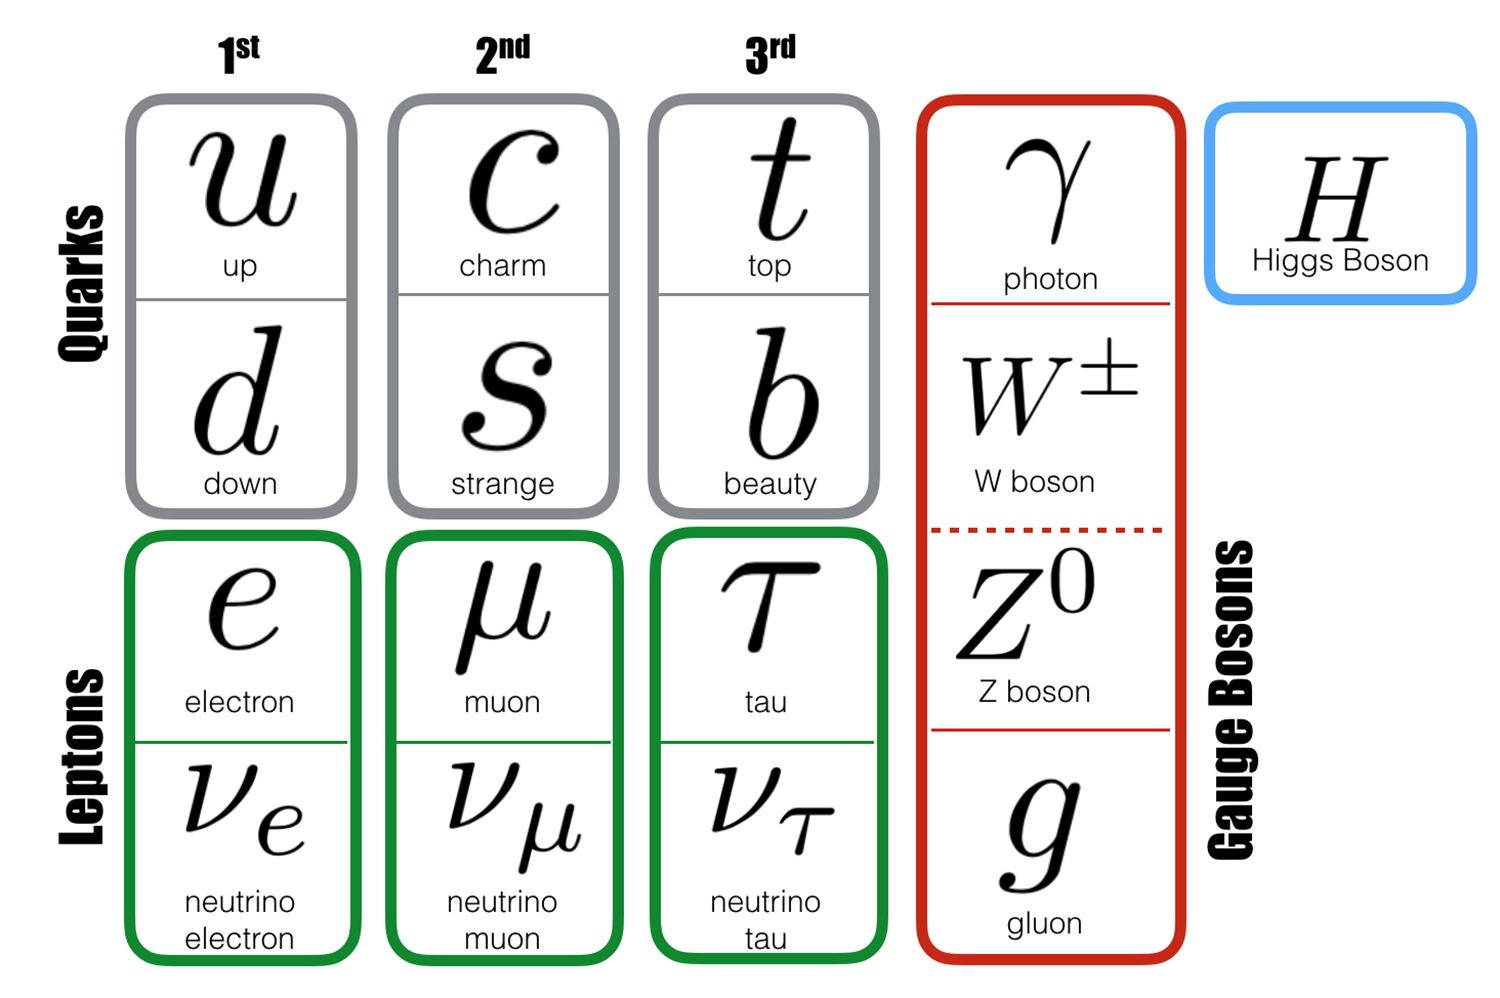
\includegraphics[width=0.80\linewidth]{figs/SM.png}
  \caption{Summary of elementary SM particles. The first three columns give
           the three generations of matter particles. Image taken
           from the Physics Institute at University of 
           Zurich~\cite{zurich_SM}.}
  \label{fig:SM}
\end{figure}

The theoretical framework underlying the SM is an example of a Quantum 
Field Theory (QFT). QFTs are consistent with both quantum mechanics and
relativity. Lattice gauge theories are a kind of QFT; therefore it is
important for the reader to know a little bit about them. A solid understanding
of QFT I think can only be achieved by taking courses along with a significant
amount of self study. In my case, that self study has required multiple years,
but you're a different person, so mileage may vary.

There are a lot
of different resources one can use to learn about QFT; for example when I was a
grad student I used Peskin and Schroeder~\cite{peskin_introduction_1995}
and Srednicki~\cite{srednicki_quantum_2007}. Far and away the most pedagogical
text book I've encountered is by Schwartz~\cite{schwartz_quantum_2014}, and it's
the one I recommend to newcomer in the field.
Nowadays there are also some very high quality lectures on YouTube,
for instance a series by Tong~\cite{tongQFT}, which I found had some other nice
introductory remarks. 
A timeline of particle discoveries can be found in
Ref.~\cite{wiki_particle_discoveries}. Another detailed historical overview
of the SM is given in Chapter 1 of Ref.~\cite{griffiths_introduction_2007}.

\section{An mnemonic history of the SM}

One could argue that the beginning of the SM history coincides with the
beginnings of modern particle physics. Since that depends on unifying
relativity, quantum mechanics, and field theory, one could arguably even take
Maxwell's equations as a starting point. 
There were also many interesting ideas that were not pursued or turned out
not to be correct yet still played some role in the history; I will not
discuss these. In some cases I may miss some discoveries that were also
important but less celebrated.

Given these ambiguities and the fact
that I am not at all a real historian, 
one might call what follows an ``approximate" history.
As I was writing this, I realized that I was trying to tell a story, i.e.
to write it in a way that one development would make sense or feel
motivated given a previous development. Usually that is a bit of an
oversimplification, but it helps me remember why certain discoveries were
significant, where some nomenclature comes from, and what it means. Hopefully it
also helps reveal how physicists think, how we are led to discoveries, and
ultimately why we believe our theories. So with these advantages in mind, I
rather decided to call it a ``mnemonic" history. 

Also while I was writing this, I learned a bunch of facts that I found
interesting but are probably a bit off-topic. Hence this mnemonic history is
densely packed with footnotes. For example I decided to start listing Nobel
prizes for some reason. By the time I realized doing this is tedious and does not
teach much, I somehow already felt pot-committed, so I ended up seeing this habit
through to the bitter end. 

\subsection{The fundamentals}

% pauli, jordan etc 1920s-30s how to quantize fields. 
% Failing to have theory with infinite num of dof,
% then tomonaga, schwinger, dyson, feynman. Can renormalize, QED discovered.
%   measurement of Lamb shift 1947. Bethe has explanation that gets refined
%   in QED, helps establish QFT.
% 1970s golden age: infinites understood through
% renormalization group wilson and kadanoff.

In 1897 J.J. Thomson did experiments with cathode rays\footnote{In a small
vacuum chamber with two electrodes, if a voltage is applied between them,
electrons will move between them. Televisions used to work by cathode ray tubes,
\index{cathode ray tube} where these electrons are deflected by magnetic fields
to make images on the screen.}
from which he concluded that electric charge must be carried by particles
with high charge-to-mass ratio, the electrons\footnote{He received the 1906
Nobel in physics for this work.} 
To explain why atoms are overall electrically neutral, Thomson guessed that
electrons are distributed in a sea of positive charge, which is the
well known {\it plum pudding model}.\index{plum pudding model} This was
disproved by Rutherford in his famous gold foil
experiment~\cite{rutherford_scattering_1911}, in which he discovered
the atomic nucleus. Shortly thereafter, he discovered the
proton~\cite{rutherford_collision_1919}.
Bohr proposed his model~\cite{bohr_constitution_1913}
of hydrogen, supposing it to be made of a proton and an electron, which agreed
well with experiment\footnote{He got the 1922 Nobel for his
contributions understanding atomic structure.}. Extending this theory to 
heavier elements by supposing
they are also made of only protons and neutrons however fails, since e.g. helium
is four times as heavy as hydrogen. This difficulty would not be sorted out
until the early 1930s, when Chadwick discovered~\cite{chadwick_possible_1932}
the neutron\footnote{1935 Nobel for him.}.


These early discoveries successfully explained many details of the atom; however
the fact that atomic nuclei are made of particles with only positive or zero
electric charge still required explanation.
Hence for some time, physicists
knew there must be some {\it strong force}\index{force!strong} that opposes
Coulomb repulsion and binds nucleons into nuclei.
Such particles held together by strong interactions are called
{\it hadrons}.\index{hadron} Nowadays we also use the terms {\it meson}
\index{meson} and {\it baryon}\index{baryon} to refer to hadrons made of
two quarks and three quarks, respectively\footnote{This naming scheme
comes from particle weights. At the time, known leptons were light, 
baryons were heavy, and mesons were somewhere in the middle. In retrospect it
would have been nicer to name them something like $n$-hadrons, but alas it would
take several decades for us to see that hadrons are made of quarks.}.


One of the earliest, important discoveries of the quantized natures of particle
properties is the celebrated Stern-Gerlach
experiment~\cite{gerlach_experimentelle_1922a,gerlach_magnetische_1922b,gerlach_experimentelle_1922c}. 
In this experiment, silver atoms
are deflected by an inhomogeneous magnetic field.
Besides having demonstrated that particles have intrinsic spin, it showed that
the spin is quantized and that measurements of spins along perpendicular axes
``reset" the spin state, and it provided the first measurement of the electron
magnetic moment.


Around this time, physicists were also beginning to see the particle nature of
light. In particular, Planck proposed~\cite{Planck:1901tja} 
that light may come in discrete packets of
energy in order to avoid the \index{ultraviolet catastrophe}ultraviolet 
catastrophe\footnote{1918 Nobel.}.
Einstein took this proposal seriously~\cite{Einstein:1905cc}, 
and used it to explain the photoelectric
effect\footnote{1922 Nobel for him. Also in 1905 he published his first
papers on special relativity, as well as a paper on Brownian motion.}. 
A careful study~\cite{millikan_direct_1916} of the photoelectric effect by 
Millikan showed that
Einstein's interpretation explained the photoelectric effect well\footnote{He
got the 1923 Nobel in part for this reason.}. Finally
Compton showed\footnote{He shared the 1927 Nobel for this.} 
that light scattered from a particle shifts by the Compton
wavelength\index{wavelength!Compton}
\begin{equation}
  \lambda_c=\frac{\hbar}{2mc},
\end{equation}
where $m$ is the target particle's mass, which one can derive by assuming light
is made of particles with zero rest mass~\cite{Compton:1923zz}.
Altogether these discoveries convinced physicists light behaves as a particle
at short enough length scales, which is the usual photon.\index{photon}


If light is to be quantized, it requires a theory that knows about both quantum
mechanics and special relativity, i.e. it needs QFT. 
The standard line of thinking can be cast in this way: One starts with
the Schr\"odinger 
equation~\cite{Schrodinger:1926gei,Schrodinger:1926vbi,Schrodinger:1926qnk,Schrodinger:1926xyk}
for a spinless, non-relativistic particle
of mass $m$ in the position basis,
\index{Schr\"odinger equation}
\begin{equation}
i\hbar\partial_t\psi=-\frac{\hbar^2}{2m}\nabla^2\psi.
\end{equation}
If we instead use a relativistic Hamiltonian and square the differential
operators on each side, we get the 
{\it Klein-Gordon equation}~\cite{Klein:1926tv,gordon_comptoneffekt_1926}
\index{Klein-Gordon equation}
\begin{equation}
-\hbar^2\partial_t^2\psi=\left(-\hbar^2c^2\nabla^2+m^2c^4\right)\psi.
\end{equation} 
While this is at least relativistically sensible, one can show that this
squaring of operators
leads to state normalization being time-dependent, i.e. probability is not
conserved. The situation was finally rescued by Dirac\footnote{Dirac
and Schr\"odinger shared the 1933 Nobel.}, who realized that
one could have a relativistically sensible equation that is first-order
in its operators by introducing some matrices and a spin component
to the wavefunction~\cite{Dirac:1928hu,Dirac:1928ej}. The result is the 
{\it Dirac equation}\index{Dirac equation}
\begin{equation}
i\hbar\slashed{\partial}\psi=mc\psi.
\end{equation}

The corresponding Hamiltonian for the Dirac equation is traceless, which
tells you that the energy eigenvalues cancel out, i.e. 
it suggests there are states of
negative energy. These negative energy states indicate that the theory
has no ground state. In order to prevent this infinite cascade into increasingly
negative energies, he speculated that these infinitely many states are already
occupied, which is referred to as \index{Dirac sea}the {\it Dirac sea}; 
the Pauli exclusion principle then prevents this infinite descent. 
If an electron in the sea were excited, it would leave behind a vacancy
that would manifest itself as a positively charged particle. This was the
prediction of the existence of the \index{positron}positron, which
was discovered\footnote{1936 Nobel.} in 1932 by Anderson~\cite{Anderson:1933mb}.
Later St\"uckelberg~\cite{Stueckelberg:1941rg} and
Feynman~\cite{feynman_theory_1949} would introduce the modern interpretation
of the positron: rather than being a hole left in the Dirac sea,
the previously negative energy states are to be understood as the
positive energy states of a different particle.


One of the last kinds of fermions needed to complete our particle collection
are the neutrinos. Before 1930, there was a problem with $\beta$-decay
\index{decay!beta} 
which is any decay emitting an $e^+$ or $e^-$ from
an atomic nucleus: Energy was not conserved. In particular if one assumes
a general $\beta$-decay process functions like
\begin{equation}
  A\to B+e^-,
\end{equation}
one can use conservation of four-momentum to find the electron energy.
The measured energy was found to fluctuate and be smaller than what four-momentum
conservation delivers. Pauli
suggested\footnote{Rather than being documented in a publication, this seems to
come from a letter written by Pauli addressed to a conference in T\"ubingen.
It opens, ``Liebe Radioaktive Damen und Herren".} that this missing energy
lies with an as-yet-undetected, weakly interacting particle, the
electron neutrino. The electron neutrino would not be 
discovered\footnote{1995 Nobel.}\index{neutrino!electron}
until the mid 1950s by Cowan and Reines~\cite{Cowan:1956rrn}.

\subsection{Weak and strong forces}

\index{interaction!weak}
In the early 1930s, Fermi published\footnote{Apparently he originally attempted
to publish it in {\it Nature}, but they rejected it because
it because ``it contained speculations too remote from reality to be of interest
to the reader".} his theory of the 
\index{decay!beta}$\beta$-decay~\cite{fermi_tentativo_1934}
\begin{equation}
  n\to\text{p}+e^-+\bar{\nu}_e.
\end{equation}
He introduced an effective 4-point interaction directly linking the four
particles in the above process.
Shortly thereafter, Yukawa~\cite{yukawa_interaction_1935} put forward that this
interaction should include another field with corresponding quantum that
mediates this interaction\footnote{Nowadays we designate as
{\it Yukawa interaction} any interaction between
Dirac fields and scalar fields of the form\index{interaction!Yukawa}
$g\bar{\psi}\phi\psi$ or $g\bar{\psi}i\gamma_5\phi\psi$.}, 
sort of like how the photon mediates the
electromagnetic interaction. Another salient point of this paper is
the introduction of the {\it Yukawa potential}\index{potential!Yukawa}
giving the potential of a gauge boson of mass $m$:
\begin{equation}
  V(r)=-g^2\frac{e^{-\alpha m r}}{r}.
\end{equation}
Here $g$ is the gauge coupling and $r$ is the interaction range. One sees that
massless gauge bosons have a Coulomb-like potential, while massive ones
are suppressed exponentially\footnote{One can also show that the Fourier
transform of this potential is the propagator, which we will discuss later.},
which gives an explanation why the weak force has a short interaction range. 
Besides already hinting massive weak bosons, this paper is considered to be
one of the first theories of the strong force; from this perspective the
proton and neutron exchange massive mesons, which therefore have a limited
interaction range\footnote{1949 Nobel.}.

\begin{figure}
  \centering
  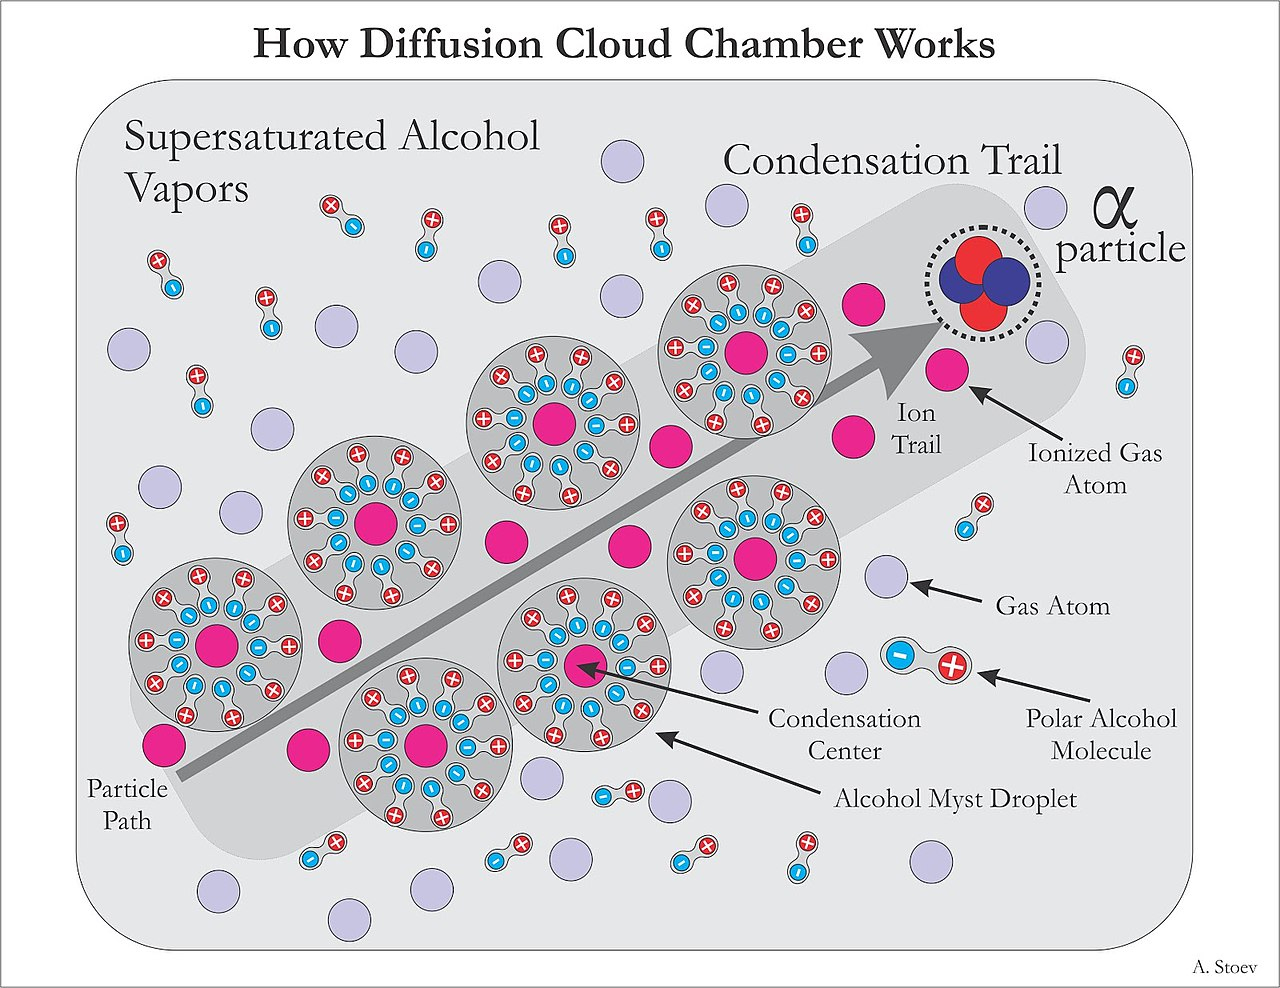
\includegraphics[width=\linewidth]{figs/Diffusion_Cloud_chamber_explained.jpg}
  \caption{Cloud chambers consist of a sealed environment with some vapor
           of e.g. alcohol. As a charged particle moves through the vapor, it knocks
           electrons off the gas; the resulting ions attract the polar molecules,
           which leaves a visible trail for a short time. To identify particles,
           you can see e.g. if they were deflected. C. T. R. Wilson is generally 
           credited as the inventor of cloud chambers, and he shared the 1927 Nobel
           in physics for it. They were extremely popular to use in experiment
           for finding particles until the later invention of the bubble chamber.
           Image taken from Wikipedia~\cite{wiki_cloud}.}
  \label{fig:cloud}
\end{figure}

An early experimental search of cosmic ray\footnote{A {\it cosmic ray} is a high
energy proton or atomic nucleus that originates somewhere from space. They were
discovered in the early 1910s by Hess, which got him the 1936 Nobel.}
\index{cosmic ray} measurements using
cloud\index{cloud chamber} chambers (see \figref{fig:cloud}) 
found the muon~\cite{neddermeyer_note_1937}, which was originally 
mistaken\footnote{Indeed the muon and pion masses are pretty close to each
other, sitting at about 106~MeV and 140~MeV, respectively.}
as the meson that Yukawa suggested. An experiment in the late 1940s showed that
the muon does not interact very strongly with atomic
nuclei~\cite{conversi_disintegration_1947}, which rules it out as the strong
force mediator. Thankfully for Yukawa the
pion\footnote{Pions\index{pion}\index{meson!pi@$\pi$} are the lightest
mesons. They are made of pairs of up and down quarks.} was
discovered~\cite{lattes_processes_1947} in 1947\footnote{And got Powell
the 1950 Nobel for it. It is actually a bit puzzling that he is the only
recipient of this prize, most obviously because only three other scientists were
on his team. Furthermore this prize credits him for his ``development of
photographic method for studying nuclear processes", even though this method was
pioneered by other physicists such as Blau and Wambacher.}.


\index{interaction!strong}
In the late 1940s and early 1950s, the {\it kaon} ($K$)~\cite{rochester_evidence_1947}
\index{meson!K@$K$} and {\it lambda} ($\Lambda$)~\cite{hopper_evidence_1950}
\index{baryon!l@$\Lambda$} hadrons were discovered. A kaon
consists of light quark and a strange, while a lambda baryon binds two light
quarks with one from a higher generation. {\it Strangeness}\footnote{We now 
\index{strangeness}
identify strangeness $S$ as
$$
  S\equiv\#\,\text{anti-strange quarks}-\#\,\text{strange quarks}.
$$}
was originally proposed as a conserved quantity to explain the relatively long
lifetimes of these particles~\cite{pais_remarks_1952,gell-mann_isotopic_1953,
pais_baryon-meson-photon_1953,tadao_charge_1953}.
Ne'eman~\cite{neeman_derivation_1961},
Gell-Mann~\cite{gell-mann_symmetries_1962}, and
Zweig~\cite{zweig_su3_1964} proposed\footnote{Gell-Mann would receive the 1969
Nobel for his contributions to understanding elementary particle
classification.} that these hadrons could be classified
according to the irreducible representations of $\SU(3)$, a viewpoint which
Gell-Mann called the \index{eightfold way}{\it eightfold way}\footnote{This
name is inspired by the eightfold path of Buddhism.}, examples of which are
illustrated graphically in \figref{fig:eightfold}. Gell-Mann
referred to the fundamental units as {\it quarks}\footnote{Gell-Mann borrows
this name from an excerpt of James Joyce's {\it Finnegan's Wake} that begins
``Three quarks for Muster Mark".
Gell-Mann was a bit of a fanciful guy I guess.}.
At first it was not clear that this quark viewpoint was more than a
purely mathematical construction, however deep inelastic
scattering\index{scattering!deep inelastic}
experiments at the Stanford Linear Accelerator (SLAC) showed that
protons are made of smaller particles, and are therefore not
elementary~\cite{bloom_high-energy_1969,breidenbach_observed_1969}.
This alone did not convince the community that quarks were 
real\footnote{For a while it was fashionable to refer to rather refer to
nucleon constituents as {\it partons}\index{parton}, a term coined
by Feynman.}, but
subsequent discoveries would solidify the quark model,
for example the 1964 discovery\cite{barnes_observation_1964} 
of the\index{baryon!$\Omega$} 
$\Omega$ baryon\footnote{An $\Omega$ baryon is any baryon not
containing $u$ or $d$ quarks. The $\Omega$ with a $t$ is not expected
to exist in the SM because the $t$ lifetime is too short to
interact strongly. The title of the discovery paper refers 
to\index{hyperon} {\it hyperons}, which are any baryons with
at least one $s$ quark. Hence $\Omega$ baryons are a type of hyperon.}.

\begin{figure}[t]
  \centering
  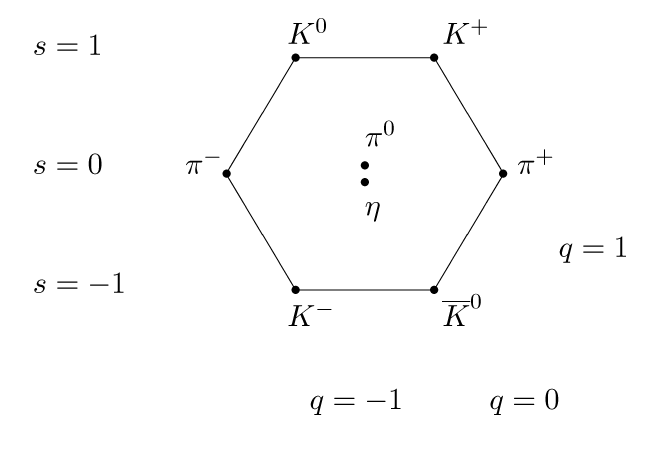
\includegraphics[width=0.48\linewidth]{figs/Meson_octet.png}
  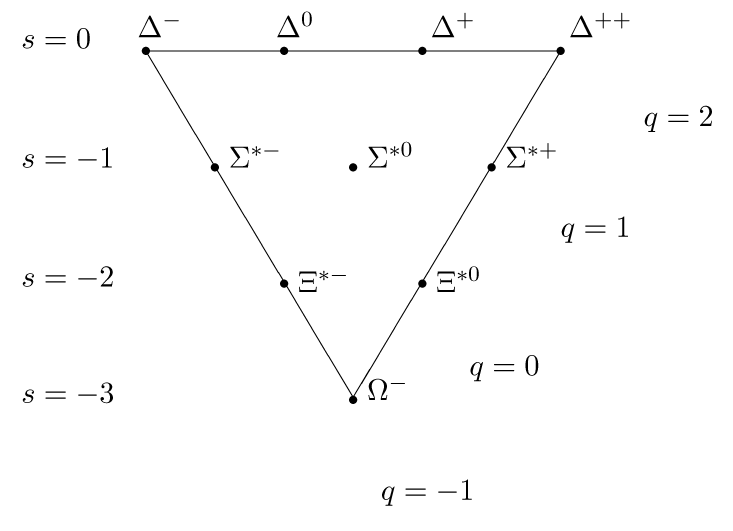
\includegraphics[width=0.48\linewidth]{figs/Baryon_decuplet.png}
  \caption{{\it Left}: Spin-0 pseudoscalar meson octet. (See
           \tabref{tab:discreteSymm} for a definition of
           pseudoscalar.) {\it Right}:
           Spin-3/2 baryon decuplet. The $s$ represents strangeness,
           with all particles in the same horizontal row having the
           same strangeness. Electric charge is represented by $q$,
           with all particles along the diagonal having the same
           electric charge. Images taken from
           Wikipedia~\cite{wiki_eightfold}.}
  \label{fig:eightfold}
\end{figure}

From here it was shown possible to formulate a QFT for the strong interaction
based on $\SU(3)$~\cite{fritzsch_advantages_1973}, which we
call quantum chromodynamics (QCD).\index{quantum chromodynamics}
The mediators are called
{\it gluons}\index{gluon} with the adjoint representation delivering
eight possible color combinations.
Gross, Wilczek~\cite{gross_d.j._ultraviolet_1973} and
Politzer~\cite{politzer_reliable_1973} demonstrated
{\it asymptotic freedom}\footnote{They got the 2004 Nobel for this.}
\index{asymptotic freedom} in this QFT, i.e. they showed that the
strong coupling decreases with increasing interaction strength, which is
consistent with the fact that one does not observe free quarks\footnote{At
least not at typical temperatures and densities.}.
This theoretical observation is buttressed by strong coupling
expansions in the lattice formulation, introduced by 
Wilson~\cite{wilson_confinement_1974}, which show that the potential
energy between two infinitely heavy quarks grows linearly with
increasing separation
(see \secref{sec:hqfe}).
%creutz_monte_1980
%wilson_RG 1 and 2

We round out this section with a short timeline of discoveries of the
remaining QCD particles. In 1974 the discovery of the
$J/\Psi$-meson\index{psion} or {\it psion}\footnote{The $J/\Psi$ consists
of a $\bar{c}c$ pair. This is also sometimes called {\it charmonium}.
\index{charmonium}} at both Brookhaven National Lab (BNL) and
SLAC~\cite{augustin_discovery_1974,aubert_experimental_1974} demonstrated
the existence of the charm quark\footnote{Richter and Ting got the 1974
Nobel prize in physics for this.}, adding further evidence to
the validity of the quark model. The $J/\Psi$ discovery marks the beginning of a
period of rapid discoveries in particle physics sometimes referred to as the
``November Revolution".\index{November Revolution} The existence of the bottom
quark was demonstrated in 1977 at Fermilab~\cite{herb_observation_1977} when the
$Y$-meson\footnote{A $Y$-meson\index{meson!Y} is a $\bar{b}b$ bound state. This is
sometimes called \index{bottomonium}{\it bottomonium}.} was discovered.
In 1979 we found experimental evidence for the
gluon via indirect observations~\cite{barber_discovery_1979} at the
Deutsches Elektronen-Synchrotron (DESY). In part because it is the
heaviest quark, the top quark would not be discovered until
1995~\cite{abachi_observation_1995,abe_observation_1995}
at Fermilab.


\subsection{Unification}


In the mid 1950s, Lee and Yang~\cite{lee_question_1956} suggested possible
experimental tests to search for parity violation in weak interaction 
processes\footnote{Lee and Yang won the 1957 Nobel prize for this.}.
Shortly thereafter, Wu et al.~\cite{wu_experimental_1957} demonstrated parity
violation in the $\beta$-decay of \ce{^{60}Co},
a result which was verified by Garwin et al.~\cite{garwin_observations_1957}. 
The theory of the weak interaction was extended by Gell-Mann and
Feynman~\cite{feynman_theory_1958} to accommodate parity violation by
introducing vector-axial currents.
That $\beta$-decay proceeds through vector-axial currents was
experimentally verified shortly thereafter~\cite{goldhaber_helicity_1958}.


The unification of the weak and electromagnetic forces began already with
Glashow in 1961~\cite{glashow_partial-symmetries_1961}, where
he puts forward the $\SU(2)\times \U(1)$ symmetry group. 
Still, this theory was not known to be renormalizable.
Also the weak interaction is short range, but this suggests that the mediating boson 
should be massive according to Yukawa. On the other hand, 
massive gauge bosons superficially spoil gauge invariance.


In superconductivity, Ginzburg-Landau theory~\cite{ginzburg_theory_1950}
gives solutions with effective mass. Nambu applied\footnote{2008 Nobel prize.} 
this to particle
physics~\cite{nambu_axial_1960,nambu_dynamical_1961,nambu_dynamical_1961-1},
but this implied the existence of Goldstone modes that are not observed.
Higgs~\cite{higgs_broken_1964} and Brout and Englert~\cite{englert_broken_1964}
noticed\footnote{Higgs and Englert received the 2013 Nobel for this.} 
that by strategically choosing 
the gauge, one can simultaneously
eliminate the Goldstone modes, add a mass term to gauge bosons, and a scalar
boson, the Higgs boson.\index{Higgs!boson}
We will discuss spontaneous symmetry breaking and Goldstone's theorem
\index{spontaneous symmetry breaking} in \secref{sec:ssb}. The Higgs
mechanism is discussed in detail in \apref{ap:spec_higgs}.


The original Higgs-Brout-Englert mechanism was demonstrated only for massive
QED; Kibble extended this idea to non-abelian
groups~\cite{kibble_symmetry_1967}. Weinberg~\cite{weinberg_model_1967}
and Salam~\cite{salam_weak_1968} applied Kibble's results to Glashow's
$\SU(2)\times\U(1)$ idea\footnote{And shared the 1979 Nobel for it.}. 
They demonstrated that one can generate masses
for weak gauge bosons along with electrons and muons, while still leaving
neutrinos massless. This approach also predicted neutral weak currents,
which were discovered shortly thereafter by the Gargamelle
experiment~\cite{hasert_observation_1974}. The $W$ and $Z$ bosons would
be discovered at the European Organization for Nuclear Research (CERN)
in the early 1980s~\cite{aubert_ratio_1983,arnison_experimental_1983}.


In 1963, Cabibbo introduced the {\it Cabibbo angle}\index{Cabibbo angle} allowing
for quark mixing in weak interactions~\cite{cabibbo_unitary_1963} to
explain the lifetimes of heavier hadrons. The suppression of flavor changing
neutral currents was explained in the early 1970s through the GIM\index{GIM mechanism}
mechanism~\cite{glashow_weak_1970}, but in order for this mechanism to work,
one needed full doublets of quarks and leptons.
Then Kobayashi and Maskawa predicted the existence of a third
generation~\cite{kobayashi_cp_1973}, since three quark generations are the
minimal amount needed to allow CP violation in the quark sector\footnote{They
shared the 2008 Nobel along with Nambu.}. The full quark mixing matrix
is known as the CKM matrix.\index{CKM matrix} Neutrino mixing is also handled
through a mixing matrix, the so-called PMNS matrix.\index{PMNS matrix} 
We discuss neutrino mixing in detail
in \apref{ap:spec_neutrino}.


In the early 1970s, t'Hooft and Veltman
showed\footnote{1999 Nobel prize for them.} these theories are
renormalizable~\cite{t_hooft_regularization_1972}. Together the Higgs mechanism
and renormalizability of the SM allow one to consistently generate gauge boson
masses while ensuring its applicability at all energy scales.
Furthermore CERN's 2012 discovery of the Higgs 
boson~\cite{aad_observation_2012,chatrchyan_observation_2012} shows that Higgs mechanism
corresponds to reality, rather than being just a mathematical trick to 
consistently approach massive elementary particles.



\section{Introductory remarks about QFT} 

Here I just want to list some things that seem to be true about the universe,
and therefore our underlying theory should reflect these things. For example:
\begin{enumerate}
  \item Causal influences seem to be {\it local}, i.e. there is no
        action-at-a-distance.
  \item Elementary particles are completely and perfectly indistinguishable.
\end{enumerate}
One way to make sense of these two points is to assume the existence of 
{\it fields},\index{field} math objects whose pre-image is all space-time.
That the field value depends on its space-time coordinate allows it to be local,
and all elementary particles are viewed as excitations of the field. Since all
particles are excitations of the same object, it is therefore unsurprising that
they would be indistinguishable.

Related to point (1) above, and as already mentioned in the introduction, we
would like our theories to have this property:
\begin{enumerate}
  \setcounter{enumi}{2}
  \item QFT should be consistent with special relativity.
\end{enumerate}
Demand (3) leads in part to the Klein-Gordon and Dirac equations, and from these
we will find that particle number is not conserved.
A fundamental QFT length scale can be heuristically derived from this statement 
as follows: Consider an elementary particle in a box of length $L$. By the 
uncertainty principle, we have
\begin{equation}
  \Delta p\gtrsim \hbar/2L,
\end{equation}
which means according to relativity,
\begin{equation}
  \Delta E\gtrsim \hbar c/2L.
\end{equation}
If the energy uncertainty is large enough, i.e. large enough to support a
particle-antiparticle pair, we conclude
\begin{equation}
  \Delta E\approx 2mc^2 \gtrsim\hbar c/2L.
\end{equation}
We then introduce the Compton wavelength\footnote{I guess if
one uses $\hbar$ instead of $h$ this is rather the {\it reduced} Compton
wavelength. But I somehow always work using $\hbar$ instead of $h$, so I opted
to abuse this convention a little.}\index{wavelength!Compton}
$\lambda_c=\hbar/mc$. This argument delivers an interpretation for 
$\lambda_c$:
\begin{equation}
  L \gtrsim \lambda_c/4
\end{equation}
is a distance threshold\footnote{I have also seen $\lambda_c/2$ as the threshold,
which comes when you think the energy uncertainty only has to be large enough to
support a single particle. But in QFT particles are always created from the
vacuum in particle-antiparticle pairs due to conservation laws.} below which 
you have to worry about QFT. Below this scale, you are likely to detect
particle-antiparticle pairs of the species you are examining, which you cannot
distinguish, and it becomes difficult to speak a unique particle at all. In that
sense the Compton wavelength gives a characteristic length scale for a
particle. One can compare this with the particle's de Broglie wavelength
\index{wavelength!de Broglie}$\lambda_v=\hbar/mv$, where it behaves in a well-defined way as a wave.


%\section{The principle of stationary action}
%This section follows a fairly well known and delightful lecture by Feynman
%\cite{caltech}.

\index{limit!classical}\index{non-relativistic limit}
\section{The non-relativistic and classical limits}

In this section I briefly give some intuition for how mundane Newtonian
physics can be recovered from the more esoteric relativistic and quantum
theories. Namely \index{limit!non-relativistic} I want to focus on 
the following two phrases:
\begin{enumerate}
  \item The non-relativistic limit is $c\to\infty$.
  \item The classical limit is $\hbar\to0$.
\end{enumerate}
I don't think I have the understanding to prove anything, but at least I
can provide some ideas and examples that can make you believe these
two statements.

The non-relativistic limit is, I think, the easier to understand. When we
learn about relativity, the speed of light $c$ is taken as a ``cosmic speed
limit"; correspondingly, sending $c\to\infty$ lifts the speed limit, and
so perhaps it's not surprising that Galilean physics is recovered.
More explicitly, we can see what happens to the Lorentz factor $\gamma$ and
Einstein velocity addition formula under these limits. For the former
we find
\begin{equation}
  \lim_{c\to\infty}\gamma
  =\lim_{c\to\infty}\frac{1}{\sqrt{1-v^2/c^2}}=1,
\end{equation}
i.e. there is no longer any time dilation or length contraction.
Meanwhile when $c\gg v$, we find for the velocity addition formula 
\begin{equation}
  v_1\oplus v_2
  =\frac{v_1/c + v_2/c}{1+v_1v_2/c^2}
  \approx \frac{v_1}{c} + \frac{v_2}{c}, 
\end{equation}
i.e. it reduces to Galilean velocity addition.

For the classical limit, one can look at specific, simple examples, such as
the quantum harmonic oscillator. In QM, the energy levels of this system
are given by
\begin{equation}
  E_n=\hbar\omega\left(n+\frac{1}{2}\right).
\end{equation}
In the $\hbar\to0$ limit, one therefore sees that the differences in energy
become continuous rather than discrete. More generally one can look at
the Heisenberg uncertainty relation,
\begin{equation}
  \Delta p\Delta x\geq \frac{\hbar}{2},
\end{equation}
and when $\hbar=0$, you are once again allowed to know position and
momentum simultaneously.

% TODO: path integral classical limit

%\section{The path integral}

%\section{The Dirac equation}\index{Dirac equation}

% dirac equation
% in order to be lorentz invariant we need gamma_0
% slash notation, maybe algebra rules
% solutions to dirac eq. look like plane waves (3.45)
% helicity as interpretation of spin against momentum
% a dirac spinor can be broken down into into creation/annihilation
% operators over all possible momenta (fourier), sum over all spins,
% attached to plane wave u.

\section{Discrete symmetries}\label{sec:discreteSymm}

A general local meson operator/current/bilinear\footnote{Sometimes in lattice
QCD you see bilinears of the form $\bar{\psi}^f(x)\Gamma\psi^g(x\pm a\muh)$,
which is called a {\it point-split}\index{point-split} operator.} has the form
\begin{equation}\label{eq:mesonInterpLat}
  \bar{\psi}^f(x)\Gamma\psi^g(x)
\end{equation}
for fermion flavors $f$ and $g$.

% you can then think about what P will do to these creation/annihilation
% states and the plane waves. has the effect of swapping the top and
% bottom components of u with a flipped spatial momentum, which is
% the same as multiplying by gamma_0.
% this gives you the rule for how psi transforms, from which you can
% figure out everything else
% compare your table with p 71 of P&S 

\begin{table}\index{vector}\index{scalar}\index{pseudovector}
\index{pseudoscalar}\index{tensor}
\begin{tabularx}{\linewidth}{LCCr} \hline\hline
Type         & $J^{PC}$ & $\Gamma$ & Example particles \\\hline
scalar       & $0^{++}$ & $\id$                 &  $H$\\
pseudoscalar & $0^{-+}$ & $\gamma_5$            &  $\pi^0$, $\pi^{\pm}$\\ 
vector       & $1^{--}$ & $\gamma^\mu$          &  $\rho^0$, $\rho^{\pm}$\\ 
pseudovector & $1^{++}$ & $\gamma^\mu\gamma_5$  &  $a_1$\\ 
tensor       & $1^{+-}$ & $\sigma^{\mu\nu}$     &  $b_1$\\ 
\hline\hline
\end{tabularx}
\caption{The $J^{PC}$ for various meson currents, where $\Gamma$ indicates the
object sandwiched between the Dirac fields in \equatref{eq:mesonInterp}.
The words ``scalar", ``vector", and ``tensor" indicate how an operator
transforms under Lorentz transformations. The ``pseudo" objects have the
opposite sign changes under parity as their corresponding objects.}
\label{tab:discreteSymm}
\end{table}
\index{meson!rho@$\rho$}\index{meson!pi@$\pi$}\index{Higgs!boson}

For instance the $\rho$ meson is a vector meson\footnote{The $\rho$ meson is any 
spin-1 combination of $u$ and $d$
quarks/antiquarks, hence their designation as ``vector" mesons in
\tabref{tab:discreteSymm}. Each quark has spin-1/2, so the $\rho$ meson is the
aligned state, while the pion is the anti-aligned state. The mass of a
$\rho$ meson is much greater than the pion (more than five times greater), which
reflects the fact that under strong interactions, aligned-spin states are higher
energy states.}.

\section{Quantum electrodynamics}\label{sec:qed}
\index{quantum electrodynamics}


\section{Spontaneous symmetry breaking}\label{sec:ssb}
\index{spontaneous symmetry breaking}
We follow Section~11.1 of Peskin and 
Schroeder~\cite{peskin_introduction_1995}.
Let $\phi(x)$ denote a vector (in the mathematical sense) of $N$ real,
scalar fields $\phi^i(x)$. Then the Lagrangian
\begin{equation}
  \Lagr=\frac{1}{2}\left(\partial_\mu\phi\right)^2
        +\frac{1}{2}\mu^2\phi^2-\frac{\lambda}{4}\phi^4
       \equiv\frac{1}{2}\left(\partial_\mu\phi\right)^2
        +V(\phi)
\end{equation}
is invariant under the orthogonal group\footnote{Recall orthogonal 
transformations\index{group!orthogonal} $R$ are the ones with 
$R^TR=\id$.} O$(N)$. This is the Lagrangian of the\index{sigma model}
{\it linear sigma model}. Note that is is a generalization of $\phi^4$ theory,
but we have replaced the positive mass parameter $m^2$ with a
negative parameter $-\mu^2$ and rescaled $\lambda$ to eliminate a factor of 6.
Classically, the potential is minimized when $\phi$ lies
on an $N$-dimensional sphere of radius $\sqrt{\mu^2/\lambda}$, i.e. 
it is minimized for vectors $\phi_\text{min}$ satisfying
\begin{equation}
  \phi_\text{min}^2=\frac{\mu^2}{\lambda}.
\end{equation}
To interpret the theory, we first choose coordinates so that 
$\phi_\text{min}$ lies
entirely along the $N$ direction
\begin{equation}\label{eq:phidir}
  \phi_\text{min}=(0,0,...,0,v),
\end{equation}
where $v=\sqrt{\mu^2/\lambda}$ is the {\it vacuum expectation value} or VEV.
Then, we define a set of shifted fields $\pi_k$ and $\sigma$ relative
to this point by writing
\begin{equation}\label{eq:phishift}
  \phi(x)=\left(\pi_1(x),\pi_2(x),...,\pi_{N-1}(x),v+\sigma(x)\right)
\end{equation}
Written in terms of $\pi$, the $N-1$ dimensional vector with components
$\pi_k$, and $\sigma$, the new Lagrangian becomes
\begin{equation}\label{eq:brokenlagr}
  \Lagr=\frac{1}{2}\left(\partial_\mu\pi\right)^2
        +\frac{1}{2}\left(\partial_\mu\sigma\right)^2
        -\frac{1}{2}\left(2\mu^2\right)\sigma^2-\sqrt{\lambda}\mu\sigma^3
        -\sqrt\mu\pi^2\sigma
        -\frac{\lambda}{4}\sigma^2
        -\frac{\lambda}{2}\pi^2\sigma^2
        -\frac{\lambda}{4}\pi^4,
\end{equation}
where we have removed constant terms, because they do not change the
physics. Equation~\eqref{eq:brokenlagr} is the Lagrangian of $N-1$
massless, dynamic fields $\pi_k$ and a dynamic field $\sigma$ with mass
$\sqrt{2}\mu$. Written in this form, the original $\text{O}(N)$ symmetry
is now obscured. There is a remaining $\text{O}(N-1)$ symmetry
rotating the $\pi_k$ among themselves. This is an example of
{\it spontaneous symmetry breaking} (SSB), and we say something like
``the original $\text{O}(N)$ symmetry spontaneously breaks to
the subgroup $\text{O}(N-1)$." 

\begin{figure}[t]
\centering
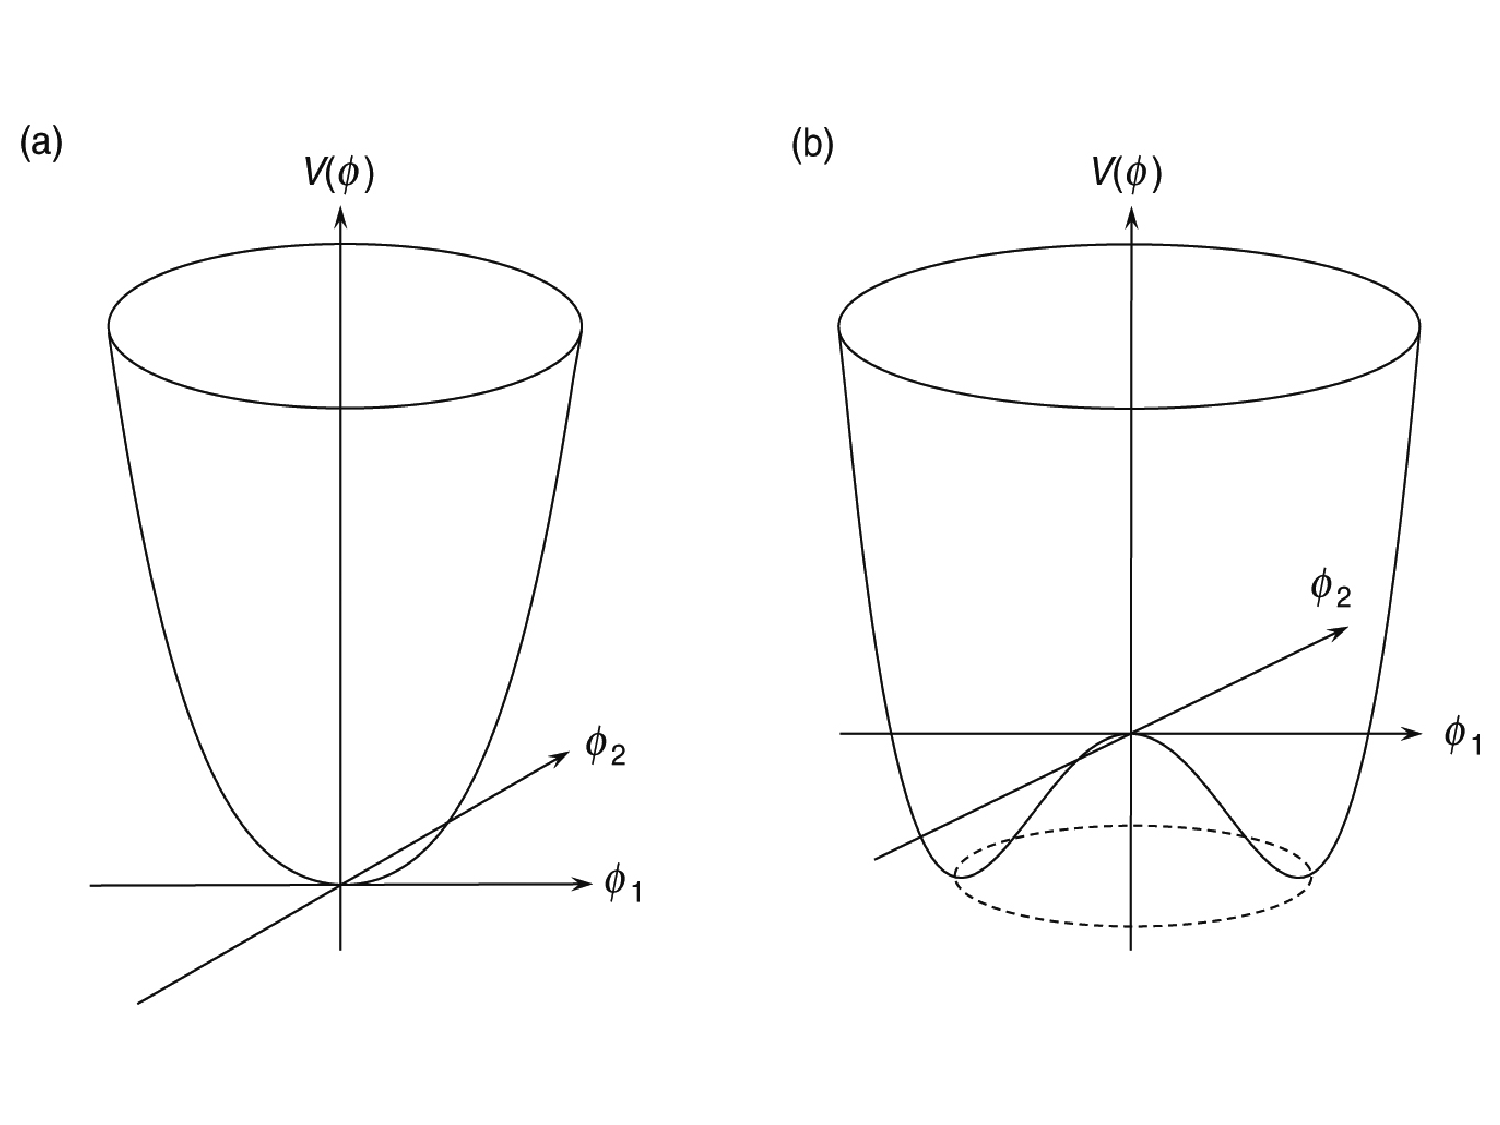
\includegraphics[width=0.8\linewidth]{figs/symm_break.pdf}
\caption{Linear sigma model potential for $N=2$. In (a) the $\phi$ field
         mass term $m^2>0$, while (b) gives this potential when
         $m^2$ is replaced by a negative parameter $-\mu^2$.
         Oscillations along the circle of minima in (b) correspond to 
         the $\pi$ field. Oscillations in the radial direction correspond
         to the $\sigma$ field. Image taken from 
         Thompson~\cite{thomson_modern_2013}.}
\label{fig:ssb}
\end{figure}

Let's try to gain some geometric intuition for this phenomenon. 
Looking at \equatref{eq:phidir}, we see that in $\phi$ space, the $\sigma$
field corresponds to oscillations of $\phi$ orthogonal to the $N-1$
dimensional hypersurface, while the massless $\pi_k$ fields
corresponds to oscillations along the hypersurface. 
An example with $N=2$ is shown in \figref{fig:ssb}. 
If we take the ground state vector~\eqref{eq:phidir} and hit it with
$\text{O}(N)$, it will be rotated somewhere else on the hypersurface.
The subgroup $\text{O}(N-1)$ hits the first $N-1$ components of the
ground state, which are all 0, thereby leaving it unchanged.
In the original $\phi^4$ theory with
$m^2>0$, the ground state vector was 0, so the $\text{O}(N)$ symmetry
was also a symmetry of the ground state. After SSB, $\text{O}(N)$ changes 
the ground state vector in general,
which is why we say the symmetry is broken. Generally any symmetry
respected by the Lagrangian but not by the ground state vector
is a broken symmetry.

In the linear sigma model, massless $\pi$ particles appeared after
SSB. This is a special example of a general result
known as Goldstone's theorem. The generated massless particles are
referred to as \index{Goldstone!boson}{\it Goldstone bosons}. 
Many light bosons can be interpreted
as approximate Goldstone bosons; as we will see in \secref{sec:cscont},
the pion can be viewed in this manner.
\begin{theorem}{Goldstone's theorem}{}
\index{Goldstone!theorem}
Consider a Lagrangian of the form
$$
  \Lagr=(\text{kinetic term for $\phi$})+
        (\text{terms independent of $\phi$})-V(\phi),
$$
where $\phi$ is the $N$-dimensional vector of real, scalar fields
$\phi_k$, and $\Lagr$ is invariant under a continuous, global
transformation of $\phi$ with generators $T^a$. Then for every
spontaneously broken generator there exists a corresponding
Goldstone boson. 
\begin{proof}
  Let $\phi_\text{min}$ be a constant field minimizing $V$. Expanding
  $V$ about this minimum we get to leading order
  $$
    V(\phi)= V(\phi_\text{min})
     +\frac{1}{2}
      (\phi-\phi_\text{min})_i(\phi-\phi_\text{min})_j\,
      \frac{\partial^2 V}{\partial\phi_i\partial\phi_j}
       \Big|_{\phi=\phi_\text{min}}.
  $$
  The differences $\phi-\phi_\text{min}$ give the new fields of the
  theory after SSB; for example in the linear sigma model this difference
  is, from \equatref{eq:phidir} and \eqref{eq:phishift},
  $$
    \phi-\phi_\text{min}=(\pi_1,...,\pi_{N-1},\sigma).
  $$
  Therefore the coefficient of the quadratic term is a symmetric matrix
  whose eigenvalues give the masses of these fields. If we can prove
  that each broken generator implies a zero eigenvalue for this matrix,
  we are done.
  The kinetic term for $\phi$ is already invariant under the global
  transformation, so if $\Lagr$ is invariant, it follows that $V$ must
  be as well. Then we can write
  $$
    V\left((\id-i\omega^aT^a)\phi\right)=V(\phi),
  $$
  where $\omega$ is some infinitesimal parameter. Expanding to linear
  order yields
  $$
    \frac{\partial V}{\partial\phi_j}(T^a\phi)_j=0.
  $$
  Differentiating the above with respect to $\phi_i$ and evaluating at
  $\phi_\text{min}$ gives
  $$
     \frac{\partial^2 V}{\partial\phi_i\partial\phi_j}
      \Big|_{\phi=\phi_\text{min}}(T^a\phi_\text{min})_j=0,
  $$
  i.e. $T^a\phi_\text{min}$ is annihilated by the mass matrix. 
  If $T^a$ is a broken generator, we have $T^a\phi_\text{min}\neq0$,
  so the above equation implies $T^a\phi_\text{min}$ is an
  eigenvector of the mass matrix with eigenvalue zero.
\end{proof}
\end{theorem}

Note that from \tabref{tab:lie}, the difference between the number of generators
of $\ON(N)$ and $\ON(N-1)$ is $N-1$, which is consistent with $N-1$ pions.


\section{Isospin and hypercharge}\label{sec:isohyper}
\index{hypercharge}\index{isospin}

We follow Chapter~9 of 
Ref.~\cite{thomson_modern_2013}. 
In quantum mechanics you learn that spin is a quantum number of
charged particles. For example the electron is a spin-1/2 particle. The
$z$-component $S_3$ of the spin operator $S$ commutes with the Hamiltonian, and
you learn that the eigenvectors of $S_3$ are the +1/2 and -1/2 states. You also
learn that the components of $S$ are related to the Pauli matrices by
\begin{equation}
  S_i=\frac{\hbar}{2}\sigma_i.
\end{equation}

Early on in nuclear physics, scientists noticed that the proton and neutron had
about the same mass, and that the nuclear force between two nucleons (i.e.
protons or neutrons) was approximately charge independent. Therefore Heisenberg
suggested that protons and neutrons were two states of a single particle (the
nucleon) just as there are spin-up and spin-down states of a spin-1/2
particle.
The quantum number corresponding to this property is called {\it isospin}.
Using this idea, the proton and neutron form an isospin doublet with total
isospin $I=1/2$ and $z$-component $I_3=\pm1/2$. Thus the Pauli matrices also
give a suitable representation of the isospin operator, and we write
\begin{equation}
  I^2=\sum\limits_{i=1}^3 I_i^2, \qquad I_i=\frac{1}{2}\sigma_i.
\end{equation}
I know this is sloppy, but I want to leave it to the reader to determine from
context whether $I$ represents the operator or the eigenvalue. 

The concept of isospin can be extended in the same way to quarks. 
In the simplest case we have $N_f=2$ and consider the lightest quarks
$u$ and $d$. The $\SU(2)$ isospin symmetry is only approximate because 
the $u$ and $d$ quarks have slightly different masses. The isospin 
doublet then has a $u$ component and a $d$ component. Generally with
$N_f$ flavors of fermion with degenerate masses, the symmetry group is 
$\SU(N_f)$ and we
form $N_f$-component multiplets in flavor space, one component per flavor.

Let's introduce the $s$ quark, assuming it has the same mass as the
$u$ and $d$ quarks, and do the $N_f=3$ case.
Using the Pauli matrices and the fact that $\SU(3)$ has 8 generators, you can
figure out what the Gell-Mann matrices are. We will say that $u$, $d$, and $s$
are eigenvectors of isospin and write
\begin{equation}
  u=\colvec{3}{1}{0}{0}, \qquad
  d=\colvec{3}{0}{1}{0}, \qquad
  s=\colvec{3}{0}{0}{1}.
\end{equation}
Then $u$ and $d$ span a 2D subspace of flavor space, so from the earlier
discussion we should know that the generators of $\SU(2)$ are contained in the
generators of $\SU(3)$. Hence
\begin{equation}
  \lambda_1=\left(\begin{array}{ccc}
            0 & 1 &  \\
            1 & 0 &  \\
              &   & 0
            \end{array}\right), \qquad
  \lambda_2=\left(\begin{array}{ccc}
            0 & -i &  \\
            i & 0  &  \\
              &    & 0
            \end{array}\right), \qquad
  \lambda_3=\left(\begin{array}{ccc}
            1 & 0  &  \\
            0 & -1 &  \\
              &    & 0
            \end{array}\right).
\end{equation}
But there's nothing special about $u$ and $d$; $u$ and $s$ will similarly form
a subspace, and so will $d$ and $s$. In both cases, we will use the Pauli
matrices as generators. We can similarly write
\begin{equation}
  \lambda_4=\left(\begin{array}{ccc}
            0 &   & 1\\
              & 0 &  \\
            1 &   & 0
            \end{array}\right), \qquad
  \lambda_5=\left(\begin{array}{ccc}
            0 &    & -i \\
              & 0  &    \\
            i &    & 0
            \end{array}\right), \qquad
  \lambda_X=\left(\begin{array}{ccc}
            1 &    & 0 \\
              & 0  &   \\
            0 &    & -1
            \end{array}\right),
\end{equation}
\begin{equation}
  \lambda_6=\left(\begin{array}{ccc}
            0 &   &  \\
              & 0 & 1\\
              & 1 & 0
            \end{array}\right), \qquad
  \lambda_7=\left(\begin{array}{ccc}
            0 &    &   \\
              & 0  & -i\\
              & i  & 0
            \end{array}\right), \qquad
  \lambda_Y=\left(\begin{array}{ccc}
           0  &    &  \\
              & 1  & 0\\
              & 0  & -1 
            \end{array}\right).
\end{equation}
Finally note the fact that there are only 8 linearly independent generators, so
two of these matrices should be linearly dependent. Since the
$u\leftrightarrow d$ isospin symmetry is the closest to being exact, we choose
the last generator to be a linear combination of $\lambda_X$ and $\lambda_Y$
that treats the $u$ and $d$ quarks symmetrically. Thus
\begin{equation}
  \lambda_8=\frac{1}{\sqrt{3}}\lambda_X+\frac{1}{\sqrt{3}}\lambda_Y
           =\frac{1}{\sqrt{3}}\left(\begin{array}{ccc}
            1 &   &   \\
              & 1 &   \\
              &   & -2
            \end{array}\right).
\end{equation}
The new isospin and total isospin operators are
\begin{equation}
  I^2=\frac{1}{4}\sum\limits_{i=1}^8 I_i^2, \qquad I_i=\frac{1}{2}\lambda_i.
\end{equation}

In the case of $\SU(2)$, the operators $I_i$ do not commute, and therefore are
not simultaneously diagonalizable. For $\SU(3)$ in the Gell-Mann basis,
$I_3$ and $I_8$ are both diagonal, so they correspond to compatible
observables. The observable $I_3$ is itself sometimes referred to
as isospin or weak isospin. The observable we associate with $I_8$ is rescaled as
\begin{equation}
  Y=\frac{1}{\sqrt{3}}\lambda_8,
\end{equation}
and $Y$ is called the {\it hypercharge}.\index{hypercharge} 
We can quickly obtain the isopins and hypercharges of
our lightest quarks: 
\begin{equation}\begin{aligned}
\hat{I_3}\,u =\frac{1}{2}u ~~~ &\text{and}~~~\hat{Y}u=\frac{1}{3}u,\\
\hat{I_3}\,d =-\frac{1}{2}d ~~~ &\text{and}~~~\hat{Y}d=\frac{1}{3}d,\\
\hat{I_3}\,s = 0           ~~~ &\text{and}~~~\hat{Y}s=-\frac{2}{3}s.
\end{aligned}\end{equation}
One can summarize this pattern of conserved charges in the following formula:
\begin{theorem}{Gell-Mann-Nishijima Formula}{}
\index{Gell-Mann-Nishijima formula}
  The electric charge $Q$ of a particle is related to its isospin and
  hypercharge by
  \begin{equation*}
    Q=I_3+\frac{1}{2}Y
  \end{equation*}
\end{theorem}


\section{Chiral symmetry}\label{sec:cscont}
\index{chiral symmetry}

There are some interesting, approximate global symmetries of the QCD Lagrangian
that crop up in the limit of zero quark mass. They are related to isospin
discussed in \secref{sec:isohyper}. Introducing small quark masses breaks this
symmetry; hence from the perspective of an effective theory of bound states we
can find something like Goldstone bosons in accordance with the discussion in
\secref{sec:ssb}. 
In this section we work with a Euclidean metric. We follow
Chapter 7 of Gattringer and
Lang~\cite{gattringer_quantum_2010}.

The massless fermion action for a single flavor reads
\begin{equation}
S_F=\int\dd[4]{x}\Lagr_F=\int\dd[4]{x}\bar{\psi}\slashed{D}\psi. 
\end{equation}
We refer to $\slashed{D}$ as the {\it massless Dirac operator}. A
\index{rotation!chiral}
{\it chiral rotation}\footnote{You may notice that the sign in the exponent
is the same for both the spinor field and its conjugate field. This is a
common feature whenever a $\gamma_5$ is in the exponent. Recall that
$\bar{\psi}=\psi^\dagger\gamma_4$. The $\gamma_5$ will anticommute with
$\gamma_4$.} of the fermion fields is a transformation
mapping
\begin{equation}
  \psi\to e^{i\alpha\gamma_5}\psi~~~~\text{and}~~~~
  \bar{\psi}\to\bar\psi e^{i\alpha\gamma_5},
\end{equation}
where $\alpha\in\R$. This is called a chiral rotation
because $\gamma_5$, which is used to define the operators~\eqref{eq:projdef},
projects out the left-handed and right-handed components of the
fermion field according to \equatref{eq:projact}. 
Using identity 2 of
\propref{prp:gammatech}, we find that $\Lagr_F$ transforms under this
rotation as
\begin{equation}
  \Lagr_F\to\bar{\psi}e^{i\alpha\gamma_5}\slashed{D}e^{i\alpha\gamma_5}\psi
         =\bar{\psi}e^{i\alpha\gamma_5}e^{-i\alpha\gamma_5}\slashed{D}\psi
         =\Lagr_F,
\end{equation}
i.e. it is invariant under chiral rotations. Using
\propref{prp:projection}, one can decompose $\Lagr_F$ into its
left-handed and right-handed parts as
\begin{equation}
  \Lagr_F=\bar{\psi}_L\slashed{D}\psi_L
         +\bar{\psi}_R\slashed{D}\psi_R,
\end{equation}
and we colloquially say that the chiral components of
$\Lagr_F$ ``do not talk to each other."
If one were to include a mass term in $\Lagr_F$, it would decompose as
\begin{equation}
  m\bar{\psi}\psi=m\left(\bar{\psi}_R\psi_L+\bar{\psi}_L\psi_R\right),
\end{equation}
which mixes the chiral components, thereby breaking chiral symmetry.
\index{limit!chiral}
This is why one refers to the limit $m\to0$ as the {\it chiral limit}.


We now generalize these ideas to $N_f$ flavors of fermion.
In general we can write a fermion action as
\begin{equation}\label{eq:nfact}
  S_F=\int\dd[4]{x}\Lagr_F=\int\dd[4]{x}
         \bar{\psi}\left(\slashed{D}+M\right)\psi,
\end{equation}
where $M$ is the {\it mass matrix}\index{mass matrix}
\begin{equation}
  M~``="~\diag(m_1,m_2,...,m_{N_f})
\end{equation}
acting in flavor space. Here the $\psi$ can be thought of as a vector with $N_f$
components $\psi_f$ like
\begin{equation}
  \psi=\colvec{4}{\psi_1}{\psi_2}{\vdots}{\psi_{N_f}}.
\end{equation}
Each $\psi_f$ is a 4-component Dirac spinor, and so $M$ has the form 
\begin{equation}
  M=\left(\begin{array}{cccc}
      m_1\id_4 &          &        & \\
               & m_2\id_4 &        & \\
               &          & \ddots & \\
               &          &        & m_{N_f}\id_4
    \end{array}\right).
\end{equation}
Similarly when we write $\gamma_\mu$ in \equatref{eq:nfact} what we really mean is
\begin{equation}
  \gamma_\mu
            =\left(\begin{array}{cccc}
               \gamma_\mu &            &        & \\
                          & \gamma_\mu &        & \\
                          &            & \ddots & \\
                          &            &        & \gamma_\mu
               \end{array}\right).
\end{equation}
Where the $\gamma^\mu$ in the matrix are defined as usual while the $\gamma_\mu$
on the LHS is just a shorthand. I'm sorry about this confusing notation. 

In the chiral limit, the action \equatref{eq:nfact} is again invariant under
\index{rotation!axial vector}
{\it axial} rotations taking the form
\begin{gather}
  \label{eq:SUNfc}
  \psi\to e^{i\gamma_5\alpha^a T^a}\psi,\qquad
    \bar{\psi}\to\bar{\psi}e^{i\gamma_5\alpha^a T^a}, \\
  \label{eq:U1A}
  \psi\to e^{i\alpha\gamma_5 \id}\psi,\qquad
    \bar{\psi}\to\bar{\psi}e^{i\alpha\gamma_5 \id},
\end{gather}
where the $T^a$ are the $N_f^2-1$ generators of $\SU(N_f)$,
$\id\equiv\id_{4N_f}$, and again $\alpha^a,\alpha\in\R$.
In this limit the action is also invariant under 
the \index{rotation!vector}{\it vector rotations}
\begin{gather}
  \label{eq:SUNf}
  \psi\to e^{i\alpha^a T^a}\psi,\qquad
    \bar{\psi}\to\bar{\psi}e^{-i\alpha^a T^a}, \\
  \label{eq:U1V}
  \psi\to e^{i\alpha \id}\psi,\qquad
    \bar{\psi}\to\bar{\psi}e^{-i\alpha \id}.
\end{gather}
The corresponding Noether currents for these symmetries are, up to a sign,
respectively
\begin{equation}\begin{aligned}
J^{5a}_\mu&=\psibar T^a\gamma_\mu\gamma^5\psi,\\
J^5_\mu&=\psibar\gamma_\mu\gamma^5\psi,\\
J^a_\mu&=\psibar T^a\gamma_\mu\psi,\\
J_\mu&=\psibar\gamma_\mu\psi.\\
\end{aligned}\end{equation}

Using eqs.~\eqref{eq:SUNfc} and \eqref{eq:SUNf}, we can define a general
chiral rotation\index{rotation!chiral} by
\begin{equation}\label{eq:chiralRotation}
  \psi\to e^{i(\alpha^a + \gamma_5\beta^a)T^a}\psi.
\end{equation}
If we take $\beta^a=0$ in \equatref{eq:chiralRotation}, we get the diagonal
isospin subgroup.
If we express the action~\eqref{eq:nfact} in terms of left-handed and
right-handed components of $\psi$, we will find that, in the chiral limit, the 
rotation~\eqref{eq:chiralRotation} can be decomposed into two $\SU(2)$
rotations, one rotating the left-handed fields of different flavors
among themselves and similarly for right-handed fields. This reflects
\begin{equation}
\SU(2)_V\times\SU(2)_A = \SU(2)_L\times\SU(2)_R.
\end{equation}

The invariance under eqs.~\eqref{eq:SUNf} and \eqref{eq:U1V} extends to the case of degenerate
masses, when $m_1=m_2=...=m_{N_f}\equiv m$, and is the familiar isospin
symmetry generalized to $N_f$ flavors. The symmetry~\eqref{eq:U1V} holds for
\index{baryon number}
arbitrary masses, and the corresponding Noether current suggests
the conserved quantity in QCD is the 
{\it baryon number}\footnote{You can see why it's called baryon number: 
A baryon is made of 3
quarks, and hence has $B=1$. Anti-quarks have $B=-1$, and
mesons have $B=0$.}
\begin{equation}
    B=\frac{1}{3}(n_q-n_{\bar{q}}).
\end{equation}


Returning once again to the massless limit, the invariance of the action under
\equatref{eq:SUNfc}, \eqref{eq:U1A}, \eqref{eq:SUNf}, and \eqref{eq:U1V}
represents the global symmetry group
\begin{equation}\label{eq:SMfglobal}
  \SU(N_f)_L\times\SU(N_f)_R\times\U(1)_V\times\U(1)_A.
\end{equation}
Breaking the global symmetry group~\eqref{eq:SMfglobal} has important
implications in QCD phenomenology. For example we will show that in the
quantized, massless theory the fermion determinant changes
under~\equatref{eq:U1A}, breaking the $\U(1)_A$ symmetry explicitly. The remaining
symmetry is
\begin{equation}\label{eq:SMglobalbUA}
  \SU(N_f)_L\times\SU(N_f)_R\times\U(1)_V.
\end{equation}
If the fermion masses are degenerate, the symmetry $\SU(N_f)_L\times\SU(N_f)_R$
breaks to its subgroup $\SU(N_f)_V$. Now the remaining symmetry is
\begin{equation}
  \SU(N_f)_V\times\U(1)_V.
\end{equation}
Finally allowing non-degenerate masses breaks the symmetry further.
There remains
\begin{equation}
  \underbrace{\U(1)_V\times\U(1)_V\times...\times\U(1)_V}_\text{$N_f$ times}.
\end{equation}

The typical QCD scale\footnote{Think of protons, which have a mass of about
940~MeV.} is $\sim1~\text{GeV}$ 
so the $u$, $d$, and $s$ quarks have masses that
are relatively small (about 5~MeV, 5~MeV, and 100~MeV, respectively).
Since these masses are so close to zero on this scale, we can say that
when $N_f=2$, and partly for $N_f=3$, \equatref{eq:SMglobalbUA} is
an approximate symmetry. If the $u$ and $d$ quarks were massless, this symmetry
would be exact, and it can be argued~\cite{gattringer_quantum_2010} that
a nucleon and its negative parity partner should have the same mass.
However one finds the negative parity nucleon to have
a mass of about 1535~MeV, and this difference of about 600~MeV is too large to
be explained by the slight breaking due to the $u$ and $d$ masses. We
conclude that something else is happening. This is another example
of SSB: If quarks were massless, the pions would arise as
the Goldstone bosons of chiral SSB; hence we refer to pions as
``would-be" Goldstone bosons.

\subsection{Chiral perturbation theory}

Let us try to understand the situation with only two light quarks $u$ and $d$.
As discussed above, introducing massive, degenerate fermions introduces a
symmetry-breaking pattern
\begin{equation}
\SU(2)_L\times\SU(2)_R\to\SU(2)_V,
\end{equation}
which is the isospin symmetry. Inspired by Goldstone's theorem, we would like to
find an effective model in which this symmetry-breaking pattern lets us clearly see
the pions as Goldstone bosons. We will use the linear sigma model as guide.
This presentation follows Ref.~\cite{schwartz_quantum_2014}.

Let $g_L\in\SU(2)_L$ and $g_R\in\SU(2)_R$. We introduce scalar fields
$\sigma_{ij}(x)$ that transform under $\SU(2)_L\times\SU(2)_R$ as
\begin{equation}\label{eq:chiralPertRot}
\Sigma\to g_L\Sigma g_R^\dagger,\qquad
\Sigma^\dagger\to g_R\Sigma^\dagger g_L^\dagger.
\end{equation}
An effective Lagrangian for this field is given by the linear sigma model
\begin{equation}
\Lagr=\left|\partial_\mu \Sigma\right|^2+m^2|\Sigma|^2-\frac{\lambda}{4}|\Sigma|^4,
\end{equation}
where $|\Sigma|^2=\Sigma_{ij}\Sigma^\dagger_{ji}$. This Lagrangian is invariant
under the rotations~\eqref{eq:chiralPertRot}. The potential part is minimized
when
\begin{equation}
\ev{\Sigma_{ij}}=\frac{v}{\sqrt{2}}\id_2,
\end{equation}
where the scale for the VEV is $v=\sqrt{m/2\lambda}$ like before.
This choice corresponds to $\SU(2)_L\times\SU(2)_R$ breaking down
to $\SU(2)_V$. 

Next we define shifted fields $\pi^a$ and $\sigma$ relative to this point.
This time we write it as
\begin{equation}
\Sigma(x)=\frac{v+\sigma(x)}{\sqrt{2}} \exp \left(2 i \frac{\pi^a(x) \tau^a}{f_\pi}\right)
\end{equation}
with the {\it pion decay constant}\index{decay constant!pion} $f_\pi$ given by
\begin{equation}
f_\pi=\frac{2m}{\lambda}=v,
\end{equation}
which leads to a nice normalization for the pion kinetic terms.
In the limit $m\to\infty$ and $\lambda\to\infty$ holding $f_\pi$ fixed we get
\begin{equation}\label{eq:Udef}
\frac{\sqrt{2}}{v} \Sigma(x) \rightarrow U(x) \equiv \exp 
\left[2 i \frac{\pi^a \tau^a}{f_\pi}\right]=\exp \left[\frac{i}{f_\pi}
\left(\begin{array}{cc}
\pi^0 & \sqrt{2} \pi^{-} \\
\sqrt{2} \pi^{+} & -\pi^0
\end{array}\right)
\right],
\end{equation}
where $\pi^0=\pi^3$ and $\pi^\pm=(\pi^1\pm i\pi^2)\sqrt{2}$. This matrix form is
thus determined by $\SU(2)$. Note that $U^\dagger U=\id$. Furthermore it
transforms under $\SU(2)_L\times\SU(2)_R$ as
\begin{equation}
U\to g_LU g_R^\dagger.
\end{equation}

Let us now write down the most general Lagrangian involving $U$ invariant under 
$\SU(2)_L\times\SU(2)_R$. It is 
\begin{equation}\begin{aligned}\label{eq:chiralLagr}
\Lagr_\chi=\frac{F_\pi^2}{4} \operatorname{tr}\left[\left(D_\mu U\right)\left(D_\mu U\right)^{\dagger}\right] & +L_1 \operatorname{tr}\left[\left(D_\mu U\right)\left(D_\mu U\right)^{\dagger}\right]^2 \\
&+L_2 \tr \left[\left(D_\mu U\right)\left(D_\nu U\right)^{\dagger}\right] \operatorname{tr}\left[\left(D_\nu U\right)^{\dagger}\left(D_\mu U\right)\right]  \\
& +L_3 \tr\left[\left(D_\mu U\right)\left(D_\mu
U\right)^{\dagger}\left(D_\nu U\right)\left(D_\nu U\right)^{\dagger}\right]\\
&+\cdots
\end{aligned}\end{equation}
This is the {\it chiral Lagrangian}\index{chiral Lagrangian}. This form is
determined by the fact we need pairs of $g_L$ and $g_R$ to cancel. Every term
requires derivatives since terms like $U^\dagger U$ are constant and hence have
no influence on the equations of motion.
In general these covariant derivatives include EW gauge fields, but no gluons.

Plugging \equatref{eq:Udef} into \equatref{eq:chiralLagr} and expanding the
exponential we find
\begin{equation}\begin{aligned}
& \frac{F_\pi^2}{4} \tr\left[\left(D_\mu U\right)\left(D_\mu U\right)^{\dagger}\right]
=\frac{1}{2}\left(\partial_\mu \pi^0\right)\left(\partial_\mu \pi^0\right)+\left(D_\mu \pi^{+}\right)\left(D_\mu \pi^{-}\right)^{\dagger} \\
& \quad+\frac{1}{F_\pi^2}\left[-\frac{1}{3} \pi^0 \pi^0 D_\mu \pi^{+} D_\mu
\pi^{-}+\cdots\right]+\cdots
\end{aligned}\end{equation}
We thus find an expansion in powers of $f_\pi^{-2}$. This implies terms $L_i$ in
\equatref{eq:chiralLagr} are suppressed relative to the leading term.
Note that there is no pion mass term, which is consistent with them being
Goldstone bosons.

\subsection{The GMOR formula}

In this section we derive a relation between pion masses and $u$ and $d$ masses.
Chiral perturbation theory gives us a lot of useful information about pion
interactions and their interactions with the EW sector, which motivates it as a
possible starting point. The trouble is we have no pion mass term, and the
theory does not know about $u$ and $d$ quarks.

To extend $\Lagr_\chi$ to include $u$ and $d$ masses, we consider a term
\begin{equation}
\Lagr_{ud}=\psibar M \psi, \quad M=\left(\begin{array}{cc}
m_u & 0 \\
0 & m_d
\end{array}\right)
\end{equation}
with $\psi$ containing $u$ and $d$ quarks only. To avoid trashing our
$\SU(2)_L\times\SU(2)_R$ symmetry, we treat the constants $m_u$ and $m_d$ as
fields and demand that the matrix $M$ transform as
\begin{equation}
M\to g_LMg_R^\dagger.
\end{equation}
Constants treated as fields in this way are sometimes called {\it
spurions}\index{spurion}. 

\begin{figure}
\centering
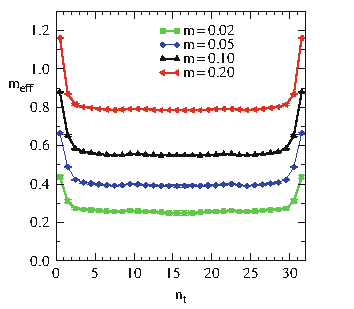
\includegraphics[width=0.5\linewidth]{figs/GMOR.pdf}
\caption{Effective pion mass extracted from pion correlation functions
for a $32^3\times16$ lattice calculation at $a\approx0.15$ fm.
Results given for different bare light quark masses. Connecting lines guide the
eye. Image taken from Ref.~\cite{gattringer_quantum_2010}.}
\label{fig:GMOR}
\end{figure}

Now we can't include the term $\Lagr_{ud}$ directly because this is a theory
where pions are the effective degrees of freedom, not the quarks. However we can
include terms with $M$ to see what happens. The leading term we can add to
$\Lagr_\chi$ looks like
\begin{equation}
\begin{aligned}
\Lagr_M & =\frac{V^3}{2} \operatorname{tr}\left(M U+M^{\dagger} U^{\dagger}\right) \\
& =V^3\left(m_u+m_d\right)-\frac{V^3}{2
F_\pi^2}\left(m_u+m_d\right)\left(\pi_0^2+\pi_1^2+\pi_2^2\right)+\order{\pi^3} .
\end{aligned}
\end{equation}
The prefactor $V^3/2$ was picked so that the VEV from $\Lagr_M$ matches the VEV
from $\Lagr_{ud}$; here $V^3=\ev{\bar{u}u}=\ev{\bar{d}d}$. Looking at coupling
for the $\pi^2$ terms, we read off the pion mass as
\begin{equation}
  M_\pi^2\approx \frac{V^3}{f_\pi^2}(m_u+m_d).
\end{equation}
This is the Gell-Mann-Oakes-Renner (GMOR)
formula~\cite{gell-mann_behavior_1968}.
It directly shows that the pion mass is not simply the sum of
the valence quark masses. Moreover since you know the physical values
of $M_\pi$, $m_u$, and $m_d$, this equation can be used to crudely estimate
$M_\pi$ for unphysical light quark masses.

In \figref{fig:GMOR} we show the results of a lattice calculation of the pion
mass taken from Ref.~\cite{gattringer_quantum_2010}. Note that increasing the
bare mass from 0.02 to 0.05 leads to a change in $m_\text{eff}$ of
$0.4/0.26\approx1.54$. From the GMOR formula, we would expect the pion mass to
change by a factor $\sqrt{0.05/0.02}\approx1.58$. Hence we see that the GMOR
formula holds to good accuracy also in lattice QCD.

\section{Anomalous magnetic moment}\label{sec:magAnom}
The {\it magnetic moment}\footnote{This is the dipole contribution to the
magnetic moment. Higher order moments, such as the quadrupole, are forbidden.
In particular this multipole expansion, which can be expressed in
terms of spherical harmonics $Y_l^m$, has its $l$ limited to $l=1$
since the only particles we consider are spin-1/2.}\index{magnetic moment} 
of a particle $X$, $\vec{M}_X$,
with $X\in\{e,\mu,\tau\}$
determines how it responds to an external magnetic field $\vec{B}$. In particular it
gives a contribution to the energy $-\vec{M}_X\cdot\vec{B}$.
The magnetic moment itself comes from the particle's intrinsic spin $\vec{S}_X$,
\begin{equation}
  \vec{M}_X=g_X\frac{q_X}{2m_X}\vec{S}_X,
\end{equation}
where $g_X$ is a constant called the {\it g-factor}\index{g-factor}
or {\it gyromagnetic ratio}\index{gyromagnetic ratio} and
$m_X$ and $q_X$ are the particle's mass and charge, respectively.
Using relativistic quantum mechanics, one can argue $g_X=2$. Any
deviation from 2 is thus called the {\it anomalous magnetic moment},
\index{magnetic moment!anomalous}
\begin{equation}
  a_X=\frac{g_X-2}{2}.
\end{equation}


\subsection{Vacuum polarization}\label{sec:VP}\index{vacuum polarization}

For this section we closely follow Ref.~\cite{maiani_hadron_2016}, 
which I found to be quite
a nice introduction to vacuum polarization.

The simplest case of {\it vacuum polarization} (VP) is a one-loop effect in
$e^+e^-$ scattering in QED. If the virtual photon has enough energy,
an $e^+e^-$ pair can be emitted and reabsorbed, and this
pair will effectively screen\footnote{The name can be remembered in analogy to
the application of an external magnetic field on a dielectric material.
In this case the polarized molecules in the material will also screen
the external field inside the material.} the electromagnetic field, reducing the force
carried by the photon.

\begin{figure}
\centering
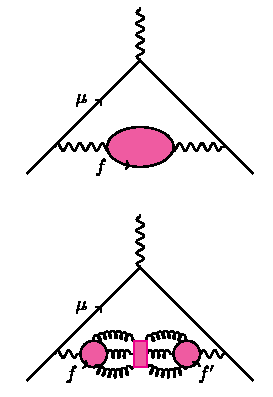
\includegraphics[width=0.8\linewidth]{figs/HVP.pdf}
\caption{HVP contribution to $a_\mu$. It arises from the two
contributions shown in this figure. {\it Top}: Quark-line
connected contribution, which is a virtual quark
bubble inserted in photon propagator. {\it Bottom}:
Quark-line disconnected contribution, which consists of
virtual quark bubbles connected by gluons. The bubbles
include all possible QED interactions.
Image taken from Ref.~\cite{FermilabLattice:2022izv}.}
\label{fig:HVPmuon}
\end{figure}


Any possible charged particle-antiparticle pair must be considered,
for instance $\mu^+\mu^-$ and $\tau^+\tau^-$. Their effects are small compared
to $e^+e^-$ due to their comparatively large masses, and are hence
only noticeable for large\index{virtuality} {\it virtuality}, or $q^2$,
of the exchanged photon. 
Contributions to VP coming from strongly interacting particles
is referred to as\index{vacuum polarization!hadronic} 
{\it hadronic vacuum polarization} (HVP).
Their effect can be computed perturbatively at large $q^2$,
but at small $q^2$ this of course fails.
The HVP contribution to $a_\mu$ is shown in \figref{fig:HVPmuon}.

The first experimental indication of HVP was found at 
LAL-Orsay~\cite{augustin_evidence_1973},
which measured the cross section for $e^+e^-\to\mu^+\mu^-$.
There a characteristic interference pattern was found for
the $\phi(1020)$ resonance\footnote{A {\it phi meson} $\phi$
is\index{meson!f@$\phi$} a strange-antistrange pair.}, in concordance with the
$\phi$ HVP contribution. CERN had a series of experiments
starting in 
1958~\cite{charpak_measurement_1961,bailey_precise_1971,bailey_anomalous_1977}, 
culminating in a measurement of $a_\mu$, which agreed at the time with the 
SM~\cite{calmet_anomalous_1977}.


Since then, higher precision was achieved at Brookhaven
and J-PARC, and a state-of-the-art determination from 
Fermilab~\cite{abi_measurement_2021}
places experimental searches at 4.2$\sigma$ tension
against data-driven theoretical methods,
which we will discuss shortly~\cite{aoyama_anomalous_2020}.


At the same time that this 4.2$\sigma$ tension was revealed,
the BMW collaboration offered a lattice calculation with precision competitive
with data-driven approaches~\cite{borsanyi_leading_2021}.
Their result tantalizingly lies between the data-driven result and experiment,
being about 2.1$\sigma$ above the theory and 1.6$\sigma$ below experiment.
Understanding this 3-fold tension requires careful investigation of
systematics. We will discuss the lattice perspective
in more detail in \secref{sec:muonAnom}. 



\section{Thirring model}\label{sec:Thirring}\index{Thirring model}

The {\it Thirring model}~\cite{thirring_soluble_1958} is a QFT in 1+1 dimensions.
Its Lagrangian density is given by
\begin{equation}
  \Lagr=\bar{\psi}(i\partial\!\!\!/-m)\psi -\frac{g}{2}
         \left(\bar{\psi}\gamma_\mu\psi\right) \left(\bar{\psi}\gamma^\mu
\psi\right).
\end{equation}
This describes a Dirac field with a self-interaction.
What's special about the massless Thirring model is that it is 
exactly solvable~\cite{johnson_solution_1961,hagen_new_1967,klaiber_1968}, 
which means it is a useful test bed for various QFT methods.
The massive Thirring model is partially solvable: my understanding is that the
correlations are not yet known.

In the context of lattice calculations, the Thirring model is used often as a
test bed for Lefshetz thimbles, which are a possible sign problem workaround.
Sometimes in these studies, one may consider a model with more or fewer spatial
dimensions.


\section{Topological invariants}\label{sec:topinvar}\index{topological!winding number}

This section follows Chapter 93 of Srednicki~\cite{srednicki_quantum_2007};
more details can be found there.
We start by considering classical, pure $\SU(2)$ gauge theory
\begin{equation}\label{eq:topaction}
  \Lagr=-\frac{1}{2g^2}F_{\mu\nu}F_{\mu\nu}
\end{equation}
at fixed $x_4$, focusing for the moment on $U$ that are time-independent.
Let $U\equiv U(\vec{x})\in\SU(2)$, and set the BC $U(\infty)=U_0$
for some constant matrix $U_0$.
The {\it topological winding number}
or {\it Pontryagin index} \index{Pontryagin index}of the map $U$ is
\begin{equation}\label{eq:wn}
  n\equiv\frac{1}{24\pi^2}\int\dd[3]{x}\epsilon_{ijk}
    \tr U\,\partial_iU^\dagger U\,\partial_jU^\dagger
        U\,\partial_kU^\dagger.
\end{equation}
The winding number is invariant under coordinate changes since the Jacobian of
the measure cancels the Jacobian of the partial derivatives.
Given the BC, it is also invariant under smooth deformations of $U$.
To show this, we first establish a useful Lemma.



\bibliographystyle{unsrtnat}
\bibliography{bibliography}

\chapter{LGT: Lattice without Fermions}\label{ch:preliminaries}

Physically, QFT is defined on a 4D Minkowskian space-time. In LGT 
the 4D space-time is instead equipped with a Euclidean metric, which is 
related to the original metric via a \index{rotation!Wick}{\it Wick rotation}
\begin{equation}
  t\to i\tau.
\end{equation} 
Therefore we will work with a Euclidean metric
and use downstairs summation indices. 
We will also use {\it natural units}\index{units!natural}
$\hbar=c=k_B=1$. In natural units, every physical
quantity has units of some power of length. For example
time has units of length, while energy, mass, and momentum
have units of inverse length. 
We first work in the continuum, then 
discretize the theory by defining the lattice.

\section{Local gauge symmetries}

Local gauge symmetries play a central role in the SM. 
Starting from a Lagrangian that depends on the derivatives of
some field, the requirement of local gauge invariance suggests that
we introduce a \index{gauge!field}{\it gauge field}. 
This gauge field allows one to define a {\it covariant derivative} 
\index{covariant derivative} whose transformation law will 
respect the local gauge symmetry.
Excitations of the gauge field are gauge bosons,
which are the force-carrying particles of the SM.

As an example consider $N_c$ complex scalar fields $\phi_{i}(x)$ equipped with 
a global $\SU(N_c)$ symmetry. The Lagrangian is
\begin{equation}\label{eq:LagrM}
  \Lagr_{M}=-\partial_{\mu}\phi^{\dagger}(x)\partial_{\mu}\phi(x)
                +m^{2}\phi^{\dagger}(x)\phi(x),
\end{equation}
where $\phi(x)$ is the $N_c$-dimensional vector formed by these fields.
$\Lagr_{M}$ becomes invariant under local $\SU(N_c)$ transformations, i.e. 
transformations of the form
\begin{equation}\label{eq:fxform}\index{gauge!transformation}
  \phi(x)\to U(x)\phi(x),
\end{equation}
where $U(x)\in \SU(N_c)$, when one replaces the partial derivative by the 
covariant derivative $D_\mu$, which transforms as
\begin{equation}\label{eq:dxform}
  D_\mu(x)\to U(x) D_{\mu}(x)U^{\dagger}(x).
\end{equation}
We define
\begin{equation}\label{eq:covariantderivative}
  D_{\mu}(x)\equiv\partial_{\mu}+A_{\mu}(x), \qquad 
       A_{\mu}(x)\equiv-igA^{a}_{\mu}(x)T^{a},
\end{equation}
where $g$ is the bare coupling constant, $A_{\mu}(x)$ is the gauge field, and 
$T^{a}$, $a=1,\dots,N^2-1$, are the generators of the $\SU(N_c)$ Lie algebra 
$\mathfrak{su}(N_c)$. For notational convenience we now suppress dependence
on $x$. 

\begin{proposition}{}{gaugecovar}
Using this definition of $D_\mu$, the gauge fields must change 
according to
$$A_{\mu}\to U A_{\mu}U^{\dagger}-(\partial_{\mu}U)U^{\dagger}.$$
%If the covariant derivative transforms as $D_\mu\to U D_\mu U^\dagger$
%under a gauge transformation, then the vector potential must
%transform as $A_\mu\to U A_\mu U^\dagger-(\partial_\mu U)U^\dagger.$
  \begin{proof} The transformed $D$ can be written
  $U D_\mu U^\dagger=\partial_\mu'+A_\mu'$. Solving for $A_\mu'$ gives
    \begin{equation*}
    \begin{aligned}
         A_\mu'
         &=U(\partial_\mu+A_\mu)U^\dagger-\partial_\mu\\
         &=U(\partial_\mu U^\dagger)
               +U A_\mu U^\dagger-\partial_\mu\\
         &=\partial_\mu-(\partial_\mu U)U^\dagger
               +U A_\mu U^\dagger-\partial_\mu\\
         &=U A_\mu U^\dagger
                -(\partial_\mu U)U^\dagger.      
    \end{aligned}
    \end{equation*}
  \end{proof}
\end{proposition}

The gauge field becomes dynamic by adding the kinetic part
\begin{equation}\label{eq:lagrkin}
  \Lagr_G=\frac{1}{4} F_{\mu\nu}^{a}F_{\mu\nu}^{a}
         =-\frac{1}{2g^2}\tr F_{\mu\nu}F_{\mu\nu},
\end{equation}
where 
\begin{equation}\label{eq:fieldstrength}
          F_{\mu\nu}^a\equiv \partial_\mu A_\nu^a-\partial_\nu A_\mu^a
                        +gf^{abc}A_\mu^b A_\nu^c,\qquad
  F_{\mu\nu}\equiv-igF_{\mu\nu}^aT^a,
\end{equation} 
and $f^{abc}$ are the structure constants of $\SU(N_c)$.
$\Lagr_{G}$ is also invariant 
under the transformation of \equatref{eq:dxform}. One way to see this
is to use the following fact.
\begin{proposition}{}{fieldtensor}
  $$F_{\mu\nu}=\left[D_\mu,D_\nu\right].$$
  \begin{proof}
    Use the definition of $D_\mu$ and apply the above commutator to some
    field $\psi$. We get
    \begin{equation*}
    \begin{aligned}
      \left[D_\mu,D_\nu\right]\psi
         &=(\partial_\mu+A_\mu)(\partial_\nu\psi+A_\nu\psi)
                     -(\mu\leftrightarrow\nu)\\
         &=\partial_{\mu\nu}\psi+\partial_\mu A_\nu\psi
           +A_\nu\partial_\mu\psi+A_\mu\partial_\nu\psi
           +A_\mu A_\nu\psi-(\mu\leftrightarrow\nu)\\
         &=\partial_\mu A_\nu\psi-\partial_\nu A_\mu\psi
           +\left[A_\mu,A_\nu\right]\psi\\
         &=-ig\left(\partial_\mu A_\mu^a-\partial_\nu A_\mu^a\right)T^a\psi
           -ig^2A_\mu^bA_\nu^cf^{bca}T^a\psi\\
         &=-ig\left(\partial_\mu A_\mu^a-\partial_\nu A_\mu^a
                    +gf^{abc}A_\mu^bA_\nu^c\right)T^a\psi\\
         &=F_{\mu\nu}\psi.
    \end{aligned}
    \end{equation*}
  \end{proof}
\end{proposition}

Taken altogether, the gauge-invariant, dynamical, 
scalar theory is described by the Lagrangian
\begin{equation}
  \Lagr=-(D_\mu\phi)^\dagger D_\mu\phi
                +m^2\phi^\dagger\phi
                -\frac{1}{2g^2}\tr F_{\mu\nu}F_{\mu\nu}.
\end{equation}
We would like
to point out that the definitions~\eqref{eq:covariantderivative} and
\eqref{eq:fieldstrength} are somewhat different than the convention
of many QFT books such as Srednicki~\cite{srednicki_quantum_2007}.
An advantage of the convention we have taken, which is also used in, 
for instance, Montvay and
M\"unster~\cite{montvay_quantum_1994}, is that one can explicitly see the
dependence of the Lagrangian~\eqref{eq:lagrkin} on the coupling. 

In this chapter we will be primarily interested in a theory with 
$\Lagr_G$ only and gauge group $\SU(N_c)$; such a theory is referred
to as {\it pure}\index{gauge!pure} $\SU(N_c)$.
Often the gauge particles of pure $\SU(N_c)$ theories are referred
to as ``gluons," even when $N_c\neq 3$. Because it
is non-Abelian, it has nonzero structure constants, which means it
contains self-interactions of the form $AAA$ and $AAAA$. 
These self-interactions are responsible for confinement, which we discuss
further in the next section. 
For the purpose of a lattice study,
it is helpful to look at a non-Abelian theory, which
has a well-defined continuum limit.

\section{Lattice regularization}\label{sec:latreg}
We now define QFT on a lattice. Let $N_{1},N_{2},N_{3},N_{4}
\in \N$. The {\it lattice} ${\LAT}$ is defined by
\begin{equation}
  {\LAT}\equiv\{x\,|\,x_\mu=a\,n_\mu,\,n_\mu\le N_\mu,\,
      \mu=1,2,3,4\}.
\end{equation}
Here $a$ is called the \index{lattice spacing}{\it lattice spacing}. 
After our Wick rotation, we identify $N_1$, $N_2$, and $N_3$
as the extensions of the lattice in the spatial directions,
and $N_4$ is taken to be the extension in the Euclidean time 
direction. Matter fields and gauge 
transformations are defined on the \index{site} {\it sites} $x\in\LAT$. We shall 
take the lattice to have periodic boundary conditions (BCs), i.e.
\begin{equation}\label{eq:PBC}
  x+aN_{\mu}\hat{\mu}=x,
\end{equation}
where $\hat{\mu}$ is the unit vector in the direction indicated by $\mu$. 
Since the lattice is discrete, one must replace partial derivatives 
by finite differences, 
\begin{equation}\label{eq:dertodiff}
  \partial_\mu f(x)\to\Delta_{\mu}f(x)\equiv\frac{f(x+a\hat{\mu})
                                                   -f(x-a\hat{\mu})}{2a},
\end{equation}
and similarly replace integrals with sums,
\begin{equation}\label{eq:inttosum}
  \int \dd[4]{x}\to a^4\sum_x.
\end{equation}
Moreover the BCs~\eqref{eq:PBC} imply for every direction
that the momentum is discretized as
\begin{equation}
  p_\mu=\frac{2\pi}{a}\frac{n_\mu}{N_\mu},
\end{equation}
which means that momentum space integrals must also be replaced by
sums
\begin{equation}
  \int\frac{\dd[4]{p}}{(2\pi)^4}\to
  \frac{1}{a^4N_1N_2N_3N_4}\sum_p. 
\end{equation}
Putting QFT on a lattice regularizes\footnote{Maybe it is worth
emphasizing here that this is a non-perturbative regularization. 
In particular, when one normally regularizes in QFT, it's because
one encounters some divergence when doing a perturbative
expansion. One then defines a regulator to parameterize this
divergence and tries to figure out which Feynman diagrams 
cancel it. In the case of LGT, the regulator is not tied to
any perturbative expansion.} the theory. 
To see this, consider a field $\phi$ defined on the lattice. 
Its Fourier transform
\begin{equation}
  \widetilde{\phi}(p)=a^4\sum_xe^{-ipx}\phi(x)
\end{equation}
is periodic in momentum space, which gives us the correspondence
$p_\mu\leftrightarrow p_\mu+2\pi/a$. Hence we can restrict
momenta to the \index{Brillouin zone}{\it first Brillouin zone},
\begin{equation}
 -\frac{\pi}{a}<p_\mu\le\frac{\pi}{a}
\end{equation}
and one obtains a UV cutoff $|p_\mu|\le\pi/a$.

Now we define the building blocks necessary to construct paths on the 
lattice. The directed {\it link}\index{link} connects $x$ with the 
neighboring point $x+a\hat{\mu}$, and its corresponding {\it link variable} 
$U_\mu(x)\in \SU(N_c)$ is defined by
\begin{equation}
  U_\mu(x)=e^{-aA_{\mu}(x)},
\end{equation}
where $A_{\mu}(x)\in\su(N_c)$. A link variable is
depicted in Fig.~\ref{fig:links} (left).
We associate to any path $\mathcal{C}$ 
the ordered product of its link variables $U(\mathcal{C})$. 
If we follow a path and then reverse our steps, we should end
up back where we started; hence
\begin{equation}
  U_{-\mu}(x+a\hat{\mu})U_\mu(x)=\id.
\end{equation}
Furthermore $U^\dagger(x)U(x)=\id$, so we can see the effect
of the dagger on link variables:
\begin{equation}
  U_\mu^\dagger(x)=U_{-\mu}(x+a\hat{\mu}).
\end{equation}
Let $\mathcal{C}_{x}$ be a path on the lattice that originates and 
terminates at the point $x$. The corresponding {\it Wilson loop} is 
defined by \index{Wilson!loop}$\tr U(\mathcal{C}_{x})$. 
Under local gauge transformations, link variables 
transform as
\begin{equation}
  U_\mu(x)\to U(x)U_\mu(x)U^{\dagger}(x+a\hat{\mu}),\qquad
  U(x)\in\SU(N_c),
\end{equation}
which ensures the gauge invariance of Wilson loops.
Maybe at this point it is worth pointing out that link variables will
have a Lorentz index attached to them (they live on the links) but
gauge transformations do not (they live on the sites). A \index{plaquette}
{\it plaquette}, shown in Figure~\ref{fig:links} (middle), is the 
smallest Wilson loop, an oriented square of side length $a$ with 
corresponding link variable 
\begin{equation}
  \plaq_{\mu\nu}(x)=U_\mu(x)U_\nu(x+a\hat{\mu})
                        U^\dagger_\mu(x+a\hat{\nu})U^\dagger_\nu(x).
\end{equation}
Every link variable in 4D LGT is part of six plaquettes\footnote{In $n$
dimensions, each site $x$ has $n!/2(n-2)!$ positively oriented plaquettes 
with a link starting at $x$ and pointing away from it. This is equal to the
number of unique combinations of directions. Each link has $2(n-1)$ staples
attached to it.}. The remaining
three edges of any particular plaquette are shaped like
a staple; therefore we call the combination
\begin{equation}\begin{aligned}\label{eq:staple}\index{staple}
  U^\sqcup_\mu(x)=
  \sum_{\nu\ne\mu}\Big[
   &U_\nu(x)U_\mu(x+a\hat{\nu})U^\dagger_\nu(x+a\hat{\mu})\\
   &+U^\dagger_\nu(x-a\hat{\nu})U_\mu(x-a\hat{\nu})
                   U_\nu(x-a\hat{\nu}+a\hat{\mu})\Big]
\end{aligned}\end{equation}
the {\it staple matrix}. A 2D staple matrix is shown in
Fig.~\ref{fig:links} (right); alternatively one can view it
as one of the three terms in the sum~\eqref{eq:staple}.

\begin{figure}[t]
  \centering
  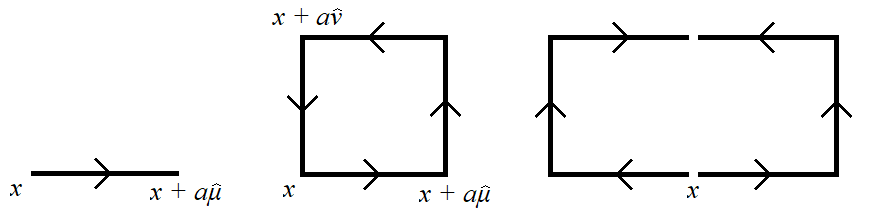
\includegraphics[width=0.9\linewidth]{figs/links.png}
  \caption{Left: A link variable. Middle: A plaquette. 
           Right: A staple matrix in 2D.}
  \label{fig:links}
\end{figure}

Plaquettes are used to construct the gauge-invariant $\SU(N_c)$ {\it Wilson
gauge action} \cite{wilson_confinement_1974}, given by
\begin{equation}\label{eq:wilsonaction}\index{Wilson!gauge action}\index{action!Wilson gauge}
    S_W\equiv\beta\sum\limits_{x;\,\mu<\nu}\left(1
         -\frac{1}{N_c}\Re\tr \plaq_{\mu\nu}(x)\right).
\end{equation}
The factor $\beta$ is given this name in analogy to the inverse temperature 
in statistical mechanics. Note that in this notation, the action has the
minimal value 0\footnote{This can be seen as follows: Go to a basis in which
$\plaq$ is diagonal. Since it is unitary, we see that its diagonal
entries must be pure phases. Hence $|\Re\tr\plaq|\leq N_c$.}. 
The Wilson action becomes identical with the
pure $\SU(N_c)$ action in the continuum limit because the plaquette is
directly related to the field tensor, which is proven in the following
proposition. 
\begin{proposition}{}{plaquette}
$$
U^\Box_{\mu\nu}(x)=\exp\left[-a^2F_{\mu\nu}(x)+\order{a^3}\right].
$$
  \begin{proof}
    Starting with the definition of the plaquette variable, we have
    \begin{equation*}\begin{aligned}
      U^\Box_{\mu\nu}(x)&=U(x,x+a\hat\nu)U(x+a\hat\nu,x+a\hat\nu+a\hat\mu)\\
               &~~~~\times U(x+a\hat\mu+a\hat\nu,x+a\hat\mu)U(x+a\hat\mu,x)\\
            &=\exp\left[aA_\nu(x)\right]
              \exp\left[aA_\mu(x+a\hat\nu)\right]\\
               &~~~~\times\exp\left[-aA_\nu(x+a\hat\mu)\right]
                \exp\left[-aA_\mu(x)\right]\\
            &=\exp\left[aA_\nu(x)\right]
               \exp\left[a\left( A_\mu(x)+a\Delta_\nu A_\mu(x) \right)
                                 +\order{a^3}\right]\\
               &~~~~\times
               \exp\left[-a\left(A_\nu(x)+a\Delta_\mu A_\nu(x) \right)
                                 +\order{a^3}\right]
               \exp\left[-aA_\mu(x)\right]\\
            &=\exp\left[aA_\nu+aA_\mu+a^2\Delta_\nu A_\mu
                 +\frac{1}{2}\left[aA_\nu,aA_\mu\right]
                 +\order{a^3}\right]\\
            &~~~~\times\exp\left[-aA_\nu-a^2\Delta_\mu A_\nu-aA_\mu
                 +\frac{1}{2}\left[-aA_\nu,-aA_\mu\right]
                 +\order{a^3}\right]\\
            &=\exp\left[a^2\Delta_\nu A_\mu+a^2\left[A_\mu,A_\nu\right]
                 -a^2\Delta_\mu A_\nu+\order{a^3}\right]\\
            &=\exp\left[-a^2F_{\mu\nu}+\order{a^3}\right].
    \end{aligned}\end{equation*}
    In the fourth step we applied the Campbell-Baker-Hausdorff formula and
    dropped the $x$ dependence for notational convenience, since at this
    step all the gauge fields depend on the same space-time point anyway.
    The fifth step uses another application of the Campbell-Baker-Hausdorff
    formula.
  \end{proof}
\end{proposition}
After some algebra, the connection between the Wilson action and the action
corresponding to \equatref{eq:lagrkin} becomes clear.
\begin{proposition}{}{} 
  $$S_W=-\frac{\beta}{4N_c}\sum_x a^4\tr F_{\mu\nu}(x)F_{\mu\nu}(x)
                  +\order{a^5}.$$
  \begin{proof} Using the definition~\eqref{eq:wilsonaction} and
    \propref{prp:plaquette} we have
    \begin{equation*}
    \begin{aligned}
      S_W&=\beta\sum_{x,\mu<\nu}\left(1-\frac{1}{N_c}\Re\tr 
            U_{\mu\nu}^\Box(x)\right)\\
         &=\beta\sum_{x,\mu<\nu}\left(1-\frac{1}{2N_c}\tr 
            \left[U_{\mu\nu}^\Box(x)+
            U_{\mu\nu}^\Box(x)^\dagger\right]\right)\\
         &=\beta\sum_{x,\mu<\nu}\left(1-\frac{1}{2N_c}\tr
            \left[2\id+\frac{a^4}{2}F_{\mu\nu}(x)^2
                  +\order{a^5}\right]\right)\\
         &=\beta\sum_{x,\mu<\nu}\left(-\frac{a^4}{2N_c}\tr F_{\mu\nu}(x)^2
                  +\order{a^5}\right)\\
         &=-\frac{\beta}{4N_c}\sum_x a^4\tr F_{\mu\nu}(x)F_{\mu\nu}(x)
                  +\order{a^5}.
    \end{aligned}
    \end{equation*}
    The cancellation of the $\order{a^2}$ term can be seen
    as follows: The role of the $\dagger$ in $\SU(N_c)$ is to take the inverse.
    For a path of link variables, this is the same as following the path
    in reverse.
    Following a plaquette in reverse just interchanges $\mu$ and $\nu$,
    which flips the sign of the leading term in the exponential
    of \propref{prp:plaquette} because $F_{\mu\nu}$
    is antisymmetric.
  \end{proof}
\end{proposition}

In the limit $a\to0$, the Wilson action coincides with the action
$S_G=\int \dd^4x\,\Lagr_G$ when one identifies 
\begin{equation}
  \beta=\frac{2N_c}{g^2}.
\end{equation}
Because of this identification, $\beta$ is also (besides $g$) sometimes 
referred to as the \index{coupling constant}{\it coupling constant}.


\section{The Haar measure}\label{sec:haar}\index{Haar measure}

We now restrict
our attention to lattices that have extension $N_1=N_2=N_3\equiv N_s$
and $N_4\equiv N_\tau$.
Expectation values of physical observables $X$ are given in 4D,
Euclidean, pure $\SU(N_c)$ LGT at zero temperature by
\begin{equation}\label{eq:0Tintegral}
  \ev{X}=\frac{1}{Z}\int\DD{U}e^{-S(U)}X(U),
\end{equation}
where the action is related to the Lagrangian by
\begin{equation}
  S=\int\dd[4]{x}\Lagr,
\end{equation}
$Z$ is the {\it partition function}
\begin{equation}
  Z\equiv\int\DD{U}e^{-S(U)},
\end{equation}
and the integration measure, the {\it Haar measure}, is
\begin{equation}
  \int\DD{U}\equiv\int\prod_{x,\mu}\dd{U_\mu(x)}.
\end{equation}
The quantities $X$ and $S$ appearing in the integral~\eqref{eq:0Tintegral}
are functionals of the configuration $U$, and this integral is
called a {\it functional integral}. The Haar measure is a product of
measures, one measure per link, each running over all possible values of
the link; in other words, the Haar measure runs over all possible
configurations\footnote{This is another advantage of the lattice formulation;
in the continuum, such integrals have an uncountably infinite dimension,
and it is hence not clear how to define them.}. The functional integral is therefore 
a weighted average of the observable $X$ over all possible configurations,
each configuration receiving a weighting factor $\int\DD{U}e^{-S}/Z$. 


We will now determine some properties of this measure. The gauge action is
invariant under gauge transformations, $U\to U'$. If we demand that the
functional integral is invariant under variable changes, we learn
\begin{equation}
  \int\DD U e^{-S(U)}
  =\int\DD U' e^{-S(U')}
  =\int\DD U' e^{-S(U)},
\end{equation}
which means
\begin{equation}
  \dd U_\mu(x)
   =\dd U_\mu(x)'=\dd\left(V(x)U_\mu(x)V(x+a\hat{\mu})^\dagger\right).
\end{equation}
Since $V(x)$ and $V(x+a\hat{\mu})$ can be chosen independently for an arbitrary
gauge transformation, it must be that
\begin{equation}\label{eq:haarcommute}
 \dd U=\dd(UV)=\dd(VU).
\end{equation}
This equation along with the normalization
\begin{equation}\label{eq:haarnorm}
  \int_{\SU(N_c)} \dd U=1
\end{equation}
are the defining properties of the Haar measure.

In what follows our integrals run over $\SU(N_c)$
and $V$ and $W$ are arbitrary $\SU(N_c)$ elements.
Using \equatref{eq:haarcommute} it follows for any 
integrable function $f$ on $\SU(N_c)$ that
\begin{equation}
  \int\dd Uf(U)=\int\dd Uf(VU)=\int\dd Uf(UV).
\end{equation}
Then using this equation, one can derive the following
useful integrals:
\begin{proposition}{}{}\label{prp:haar}
  Let $U\in\SU(N_c)$ in the fundamental representation. Then
  \begin{center}\begin{tabular}{lrcl}
  1. &$\int \dd U U_{ab}$ &=& 0;\\[1mm]
  2. &$\int \dd U U_{ab}U_{cd}$ &=& 0;\\[1mm]
  3. &$\int \dd U U_{ab}U^\dagger_{cd}$ 
       &=& $\frac{1}{N_c}\delta_{ad}\delta_{bc}$;\\[1mm]
  4. &$\int \dd U U_{ab}U_{cd}U_{ef}$ 
       &=& $\frac{1}{2 N_c}\epsilon_{ace}\epsilon_{bdf}$.
  \end{tabular}\end{center}
\end{proposition}
In \secref{sec:hqfe} we will encounter products of Wilson
loops that have one link in common. The third formula in
\propref{prp:haar} delivers the following equation, allowing
us to integrate out the common link in such situations:
\begin{equation}
  \int \dd U\tr VU\tr U^\dagger W=\frac{1}{3}\tr VW
\end{equation}

\section{Heavy quark free energy}\label{sec:hqfe}


When one thinks about the potential\footnote{At finite temperature
one distinguishes between potential energy and free energy since $F=U-TS$.}
energy between a static quark-antiquark pair, \index{static quark}
i.e. a pair of infinitely heavy quarks, one imagines
a Wilson loop $W(\mathcal{C}_{rt})$
where $\mathcal{C}_{rt}$ is a rectangular loop of side lengths 
$r$ and $t$ parallel
to the Euclidean time direction. When
viewing this Wilson loop in the temporal gauge, \index{gauge!temporal}
defined on the lattice by\footnote{In the Euclidean continuum theory,
the temporal gauge is defined by $A_4=0$.}
\begin{equation}
  U_4(x)=\id,
\end{equation}
one argues that
the edges parallel to the Euclidean time direction correspond to
a static quark-antiquark pair.
Then the {\it static quark potential}
\index{potential!static quark} $V(r)$ is defined by
\begin{equation}\label{eq:staticpotential}
  V(r)\equiv-\lim_{t\to\infty}\frac{1}{t}\log W(\mathcal{C}_{rt})  
\end{equation}
and gives the energy of the gauge field due to two color sources separated by
a distance $r$. 


We will argue the static quark potential has the form
\begin{equation}\label{eq:cornellpotential}
  V(r)=A+\frac{B}{r}+\sigma r,
\end{equation}
which is sometimes called the {\it Cornell potential}\index{potential!Cornell},
where $A$ and $B$ are constants and
$\sigma$ is the {\it string tension}\index{string!tension}. 
If the string tension is non-vanishing, then the potential scales linearly 
with $r$ in the large $r$ limit; 
this phenomenon has been observed in LGT 
simulations\footnote{Some studies are quoted in e.g.
Ref.~\cite{montvay_quantum_1994}.},
and we thus see LGT proffers an explanation of confinement.


The Coulomb-like term in \equatref{eq:cornellpotential} can be seen
mnemonically as follows. From \equatref{eq:fieldstrength}
one sees that the $\SU(N_c)$ field strength tensor has the same form
as the $\U(1)$ tensor, except for the last term, which is due to
$\SU(N_c)$ being non-abelian, and which comes with a factor $g$.
Hence in the small coupling limit, we recover the QED field
strength tensor. We know QED has a Coulomb term in its potential,
so we should a expect the $1/r$ term.


Conversely we argue for the linearly rising term in the strong
coupling limit. For arbitrary path $\mathcal{C}$ we expand the Wilson
loop expectation value as
\begin{equation}\label{eq:evWC}
  \ev{W_\mathcal{C}}=\frac{1}{Z}\int\DD U
    \exp\left(-\frac{\beta}{3}\sum_\square\Re\tr\left[\id-\plaq\right]\right)
    \tr\prod_{l\in\mathcal{C}}U_l,
\end{equation}
where the sum runs over plaquettes of some orientation and the product over
links in the Wilson loop. We factor out the sum over $\id$ appearing in the
both the numerator and the partition function to get
\begin{equation}\begin{aligned}
  \ev{W_\mathcal{C}}&=\frac{1}{Z'}\int\DD U
    \exp\left(\frac{\beta}{3}\sum_\square\Re\tr \plaq\right)
    \tr\prod_{l\in\mathcal{C}}U_l\\
                    &=\frac{1}{Z'}\int\DD U
    \exp\left(\frac{\beta}{6}\sum_\square\left(\tr \plaq+\tr
     U^{\square\,\dagger}\right)\right)
    \tr\prod_{l\in\mathcal{C}}U_l.
\end{aligned}\end{equation}
Now we expand the exponential:
\begin{equation}\begin{gathered}\label{eq:wilsonloopexpexpand}
    \exp\left(\frac{\beta}{6}\sum_\square\left(\tr \plaq+\tr
     U^{\square\,\dagger}\right)\right)~~~~~~~~~~~~~~~~~~~~
       ~~~~~~~~~~~~\\
    =\sum_{i,j=0}^{\infty}\frac{1}{i!j!}\left(\frac{\beta}{6}\right)^{i+j}
      \left(\sum_\square\tr\plaq\right)^i\left(\sum_{\square'}\tr
        U^{\square'\,\dagger}\right)^j.
\end{gathered}\end{equation}
Using this expansion, we can get the leading order contribution to the
denominator of \equatref{eq:evWC}. The zeroth order term is 1. The first
order term is zero due to the first statement of \propref{prp:haar}. Hence,
\begin{equation}
  Z'=1+\order{\beta^2}.
\end{equation}


To see where the linear behavior in \equatref{eq:cornellpotential} comes from,
we apparently need to apply this expansion to \equatref{eq:staticpotential}.
Hence we consider the rectangular contour $\mathcal{C}_{rt}$ with spatial
edge $r=an_r$ and $t=an_t$.
We will use the third statement in \propref{prp:haar} to calculate
the product of this exponential with the Wilson loop. 


The two plaquette sums
appearing in \equatref{eq:wilsonloopexpexpand} have opposite orientations, so
according to this Proposition, only one of those two sums can contribute when hitting
the Wilson loop.
\begin{figure}
  \centering
  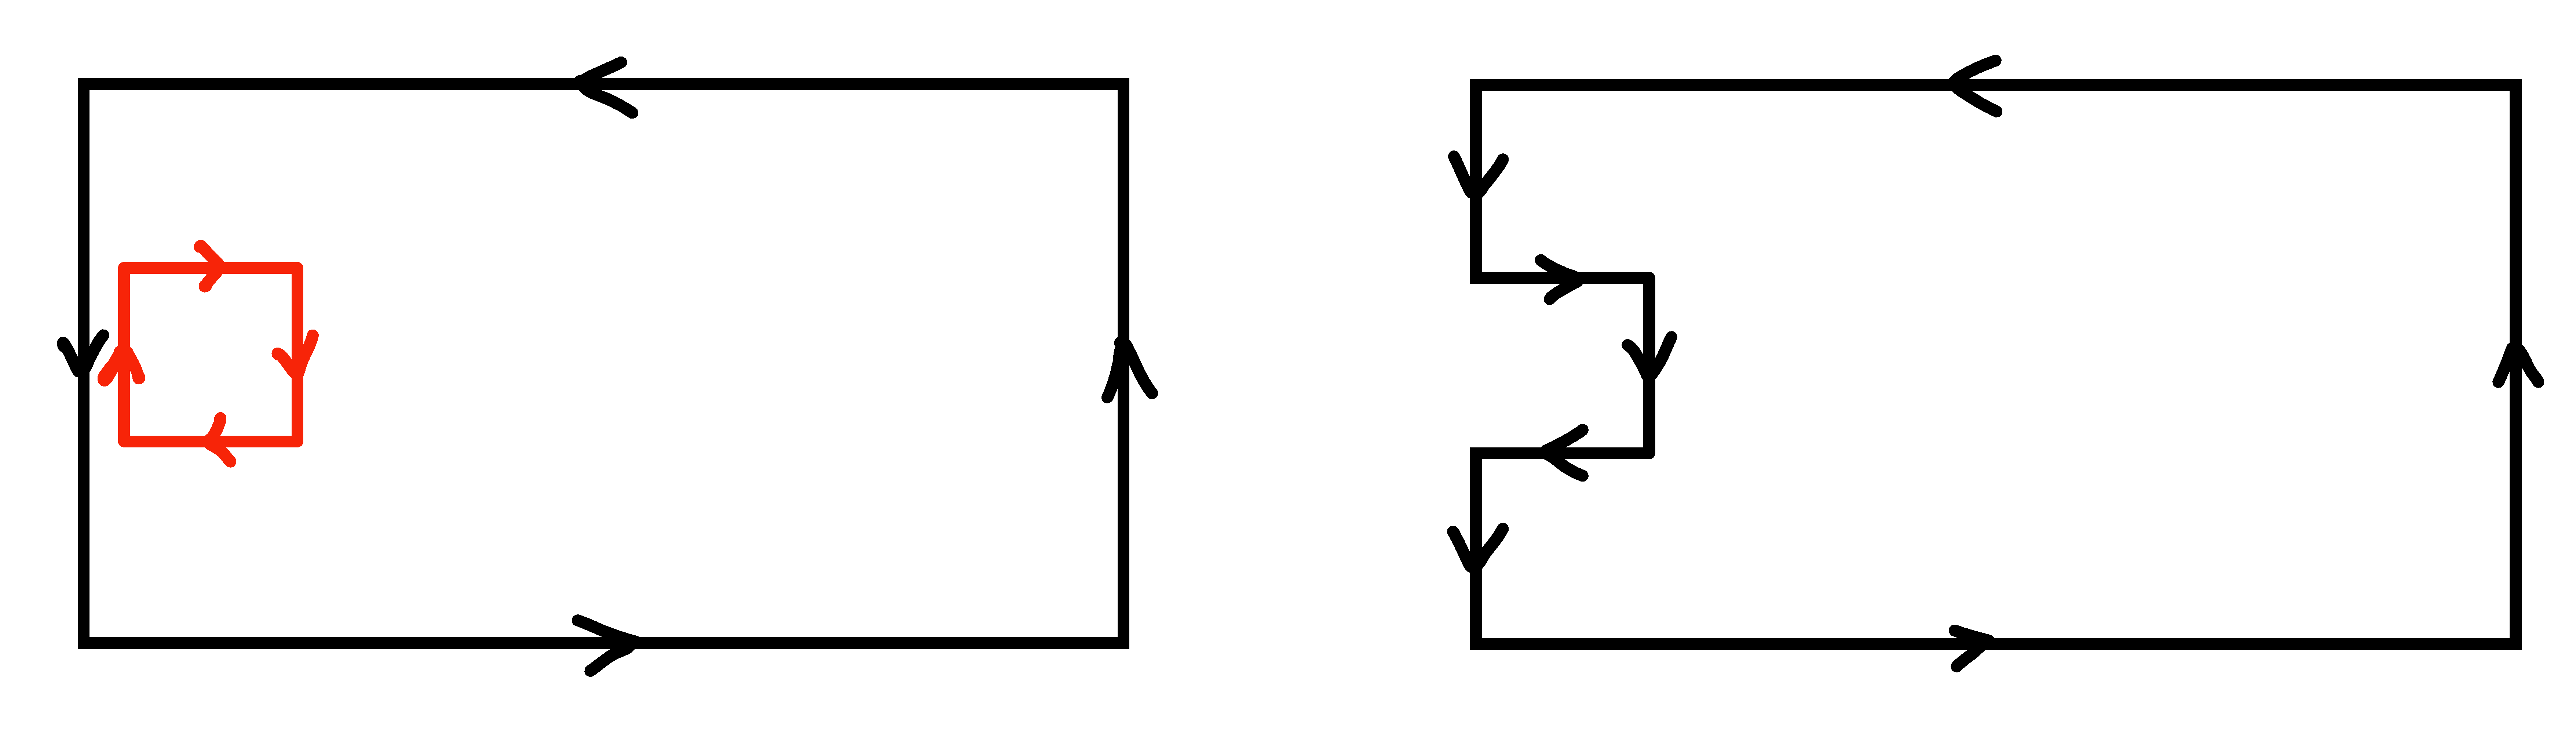
\includegraphics[width=0.9\linewidth]{figs/plaquetteTimesWilson.pdf}
  \caption{Integrating over the product of the Wilson loop $W(\mathcal{C}_{rt})$
           with an oppositely oriented plaquette. The resulting contour on the
           right comes with a factor 1/3 due to \propref{prp:haar}.}
  \label{fig:erasePlaquette}
\end{figure}
When a plaquette with non-vanishing contribution hits the loop,
the common link disappears, and the remainder of the plaquette is stitched to
the Wilson loop, as shown in \figref{fig:erasePlaquette}.
If in our sum there remains even one link that does integrate against a corresponding
plaquette, the integral will vanish according to statement 1 of
\propref{prp:haar}. Hence the only contributing terms are those terms in our
sum with a product of $n_A\equiv n_r n_r$ unique plaquettes that lie within
the boundary of the Wilson line. There are $n_A!$ such terms. Hence
\begin{equation}\begin{aligned}
  \ev{W(C_{rt})}
      &\approx\int\DD U\frac{1}{n_A!}\left(\frac{\beta}{6}\right)^{n_A}
            \left(\sum_\square\tr U^{\square\,\dagger}\right)^{n_A}
            \tr\prod_{l\in\mathcal{C}_{rt}}U_l\\
      &=\tr\id\left(\frac{\beta}{6}\right)^{n_A}\left(\frac{1}{3}\right)^{n_A}
\end{aligned}\end{equation}
If we look in the large $t$ limit and compare the above equation with 
\equatref{eq:staticpotential} we conclude at leading order in $\beta$
\begin{equation}
  V(r)\sim-\frac{r}{a^2}\log\left(\frac{\beta}{18}\right)\left(1+\order{\beta}\right)
          \equiv\sigma r,
\end{equation}
i.e. we identify this factor multiplying $r$ as the leading order expression
for the string tension. 


With static quarks, the consequence of this is that
the potential between a quark-antiquark pair diverges as you separate the pair.
With dynamical fermions, this potential energy eventually becomes larger than
the mass of a quark-antiquark pair, and it eventually becomes energetically
favorable to create such a pair out of the vacuum that binds to the two original
quarks forming two mesons. This phenomenon is known as 
{\it string breaking}\index{string!breaking}.


\section{Renormalization group and the continuum limit}
\index{renormalization!group}\index{limit!continuum}


In the limit $a\to0$, physical quantities $P$ should agree with experimental
results, which means they should become independent of $a$, ``forgetting"
about the lattice structure. Since $P$ depends in general also on $g$,
this means that changes in $a$ have to be compensated by changes in $g$
to keep the physics constant. More precisely, it must be that 
\begin{equation}
  \lim_{a\to0}P\Big(g(a),a\Big)=P_0
\end{equation}
where $P_0$ is the physical quantity's experimental value.
Both Callan~\cite{callan_broken_1970} and
Symanzik~\cite{symanzik_small_1970,symanzik_small-distance-behaviour_1971}
independently formulated the requirement of constant physics as
a differential equation
\begin{equation}\label{eq:RGflow}
  \left(\frac{\partial}{\partial\log a}
        +\frac{\partial g}{\partial\log a}
         \,\frac{\partial}{\partial g}\right)P=0. 
\end{equation}
(The RHS of this equation is more precisely
$\order{(a/\xi)^2\log(a/\xi)}$ for a lattice system
with correlation length $\xi$~\cite{montvay_quantum_1994}.)
Equation~\eqref{eq:RGflow} relates to a semi-group of scale 
changing transformations called the {\it renormalization group} (RG). 
The coefficient of the second term is called the {\it beta function},
\begin{equation}\label{eq:betafunction}\index{beta function}
  \beta\equiv-\frac{\partial g}{\partial\log a},
\end{equation}
and it measures how the bare\footnote{Usually in QFT one likes to label
a coupling that changes with some cutoff as a ``renormalized" coupling.
But in this case it really is the bare coupling that is changing with $a$.
One way to see this is that $a$ is not corresponding to any real-world
observable; the lattice spacing is just a calculational crutch. If changes
in a crutch need to be compensated by changes in another quantity,
the other quantity better also be a crutch, and indeed, bare quantities
are the ones that aren't measurable.}
coupling $g$ must change when $a$ changes.
The use of the symbol $\beta$ here is unfortunately a convention; it
is not to be confused with the coupling constant. It is usually clear
from context what is meant. 


In practice $\beta$ can be determined
from lattice perturbation theory. An explicit dependence of $g$ on $a$ is then
determined by solving the differential equation~\eqref{eq:betafunction}. 
For example the pure $\SU(N_c)$ lattice beta function\footnote{In a theory
with $N_f$ fermion flavors, the 1-loop contribution is
$$
  b_0=\left(\frac{11N_c}{3}-\frac{2N_f}{3}\right)\frac{1}{16\pi^2}.
$$
Hence when introducing fermions, at leading order, one loses asymptotic freedom
whenever $N_f\geq 11N_c/2$.} has been calculated 
up to 3-loop order in perturbation theory. It is given by
\begin{equation}\label{eq:blatgs}
  \beta_L(g)=-b_0g^3-b_1g^5-b_2^Lg^7+\order{g^{9}}
\end{equation}
where
\begin{equation}\label{eq:blat3loop}\begin{gathered}
  b_{0}= \frac{11}{3}\frac{N_c}{16\pi^2}, \qquad
  b_{1}= \frac{34}{3}\Bigg(\frac{N_c}{16\pi^2}\Bigg)^{2},\\
  b_{2}^{L}=\Bigg(-366.2+\frac{1433.8}{N_c^2}-\frac{2143.0}{N_c^4}\Bigg)
            \Bigg(\frac{N_c}{16\pi^2}\Bigg)^{3}
\end{gathered}\end{equation}
have been calculated at one-loop 
\cite{gross_d.j._ultraviolet_1973,politzer_reliable_1973}, two-loop 
\cite{belavin_calculation_1974,caswell_asymptotic_1974,jones_two-loop_1974},
and three-loop order~\cite{alle_three-loop_1997}, respectively.
The constants $b_0$ and $b_1$ are universal in the sense that they do not 
depend on the regularization scheme; however $b_2$ does depend on the
regularization scheme, with $b_2^L$ being the value using lattice
regularization. The RG equation on the lattice is
\begin{equation}
  \beta_{L}(g)=-a\dv{g}{a},
\end{equation}
and its solution is given by
\begin{equation}\label{eq:latRGEsoln}
  a\Lambda_{L}
   =\exp\Bigg(\int^g\frac{\dd g'}{\beta_{L}(g')}\Bigg) \\
   =f_{as}\big(g^2\big)
   \equiv f_{as}^0\big(g^2\big)\sum\limits_{i=0}^{\infty}
     q_i\,g^{2i},
\end{equation}
where $q_0=1$, the other $q_i$ are coefficients that can be, in 
principle, calculated perturbatively, and
\begin{equation}\label{eq:f0}
   f_{as}^0\big(g^2\big)\equiv\exp\Bigg(-\frac{1}{2b_{0}g^2}\Bigg)
    (b_{0}g^{2})^{-b_{1}/2b_{0}^{2}}.
\end{equation}
In fact from \equatref{eq:blatgs} and \eqref{eq:blat3loop}, one obtains
\begin{equation}\label{eq:q1value}
  q_1=\frac{b_{1}^{2}-b_{2}^{L}b_{0}}{2b_{0}^{3}}=
  \begin{cases}
     0.08324 & \text{for}\ \SU(2) \\
     0.18960 & \text{for}\ \SU(3).
  \end{cases}
\end{equation}
The integration constant $\Lambda_{L}$ has units of mass and is called the
{\it lattice $\Lambda$-parameter}.
From \equatref{eq:latRGEsoln} one sees that
\begin{equation}\label{eq:llat}
  \Lambda_L=\lim_{g\to0}\frac{1}{a}f_{as}^0\big(g^2\big).
\end{equation}

\begin{figure}
  \centering
  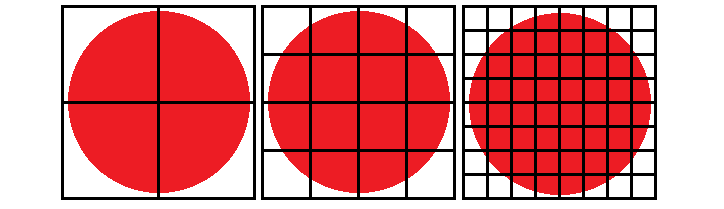
\includegraphics[width=0.9\linewidth]{figs/continuumlimit.png}
  \caption{A schematic representation of the continuum limit. The
           red object represents some physical quantity. As the
           images progress to the right, the lattice spacing decreases
           relative to the physical length, and the bare coupling
           becomes weaker.}
  \label{fig:climit}
\end{figure}

The fact that pure $\SU(N_c)$ theory has a negative beta function
\eqref{eq:blatgs} has a profound physical implication. In particular 
when we invert \equatref{eq:latRGEsoln} keeping only universal
terms, we find
\begin{equation}\label{eq:rgesoln}
  g(a)^{-2}=b_0\log\left(a^{-2}\Lambda_L^{-2}\right) 
            +\frac{b_1}{b_0}\log\log\left(a^{-2}\Lambda_L^{-2}\right)
            +\order{1/\log\left(a^2\Lambda_L^2\right)}.
\end{equation}
Two consequences are that the coupling $g(a)$ is driven to zero
as $a$ approaches zero, which is known as 
\index{asymptotic freedom}{\it asymptotic freedom}, while at low energies,
$g(a)$ becomes too large for reliable perturbative analysis.

From \equatref{eq:latRGEsoln} we see that taking $g\to0$ drives $a\to0$.
However the limit $g\to0$ is not enough to ensure a well-defined continuum
limit. The physical size of the lattice is proportional to $a^4$, and hence
collapses to zero unless we also increase the number of sites. Therefore
we extrapolate to the continuum limit by calculating our observable
of interest at different values of the coupling constant, with the 
extensions $N_1$, $N_2$, $N_3$, and $N_4$ chosen so that the physical 
size of the lattice is large enough for a reliable calculation of 
the observable of interest. A schematic representation is shown in
Figure~\ref{fig:climit}. We note that two kinds of systematic uncertainty 
arise in this context. Namely, to what extent do finite lattice
spacing (which limits the smallest wavelength) and finite lattice
size (which limits the largest wavelength) affect our results?
These questions are discussed in detail in 
\secref{sec:refscales}.

\section{Finite temperature}\label{sec:finitetemp}

The functional integral for a 3D, 
pure $\SU(2)$ LGT system in contact with a thermal reservoir at 
temperature $T$ has the same structure, except that the corresponding 
action is
\begin{equation}\label{eq:Tintegral}
  S(T)=\int_0^{1/T}\dd{x_4}\int\dd[3]{x}\Lagr,
\end{equation}
and the Haar measure runs over fields that are periodic in the
$x_4$ direction. Because the functional integral for both systems is
formally the same, we interpret a 4D system with $N_s\gg N_\tau$ as
a 3D system at finite temperature, with $x_4$ running along a 
temperature direction rather than a time direction. 
The continuum limit of the finite temperature system corresponds
to $a\to0$ with $aN_s$ and $aN_\tau$ fixed. The {\it physical
temperature}\index{temperature} is seen to be
\begin{equation}
  T=\frac{1}{aN_\tau}.
\end{equation}


\section{Scale setting}\label{sec:refscales}\index{scale!setting}


Lattice computations deliver dimensionless quantities $L=\ell/a$, where 
$\ell$ is some physical length. The requirement that the theory has a 
well-defined continuum limit means that for two length scales 
$\ell_i$ and $\ell_j$
\begin{equation}
  r_{ij}\equiv\frac{\ell_i}{\ell_j}=\lim_{a\to 0}\frac{L_i}{L_j}
        \equiv\lim_{a\to 0}R_{ij},
\end{equation}
i.e. in the continuum limit, length ratios attain their physical values.
Continuum limit extrapolations of a particular length $\ell_i$ therefore
depend on how one determines $R_{ij}$ and on the choice of the
{\it reference scale} or {\it reference length}\index{scale!reference} $\ell_j$. 
Choosing a reference scale to use for continuum limit extrapolation
is called {\it scale setting}, and commonly one says
``we set the scale with $\ell_j$."


Calculation of the constants $R_{ij}$ is prone to nontrivial statistical and
systematic errors because they come from MCMC simulations performed on 
finite lattices with nonzero spacing. Therefore it is desirable to set
the scale with a quantity that is computable with low numerical effort,
has small systematic uncertainties, and good statistical precision.
We begin by introducing some reference scales. 


\subsection{String tension}\index{string!tension}


One of the first reference scales used in lattice calculations was the string
tension. The string tension is loosely related to physics experiment; it can be
extracted from Regge trajectories, but its value in MeV is somewhat
model-dependent~\cite{smit_introduction_2002}.


\subsection{Deconfinement temperature}\index{temperature!deconfinement}


Another choice of scale for pure gauge systems is the 
{\it deconfining phase transition temperature}
\begin{equation}
  T_c=\frac{1}{a(\beta_c)\,N_\tau}.
\end{equation}
For $T<T_c$ gluons are bound into  glueballs, while 
at higher temperatures $T>T_c$ they exist in a gluon plasma. 
The deconfining phase transition is a second-order phase transition for 
$\SU(2)$~\cite{engels_critical_1996} and
and a first-order transition for $\SU(N_c)$ when $N_c>2$
~\cite{svetitsky_critical_1982}. 
The order parameter\footnote{We will argue this in \secref{sec:ploop}.} 
for this transition is the \index{Polyakov loop}
{\it Polyakov loop}\index{Polyakov loop},
\begin{equation}
  P(\vec{x})\sim\tr\prod_\tau U_4(\vec{x},\tau),
\end{equation}
which is a straight Wilson loop of length $N_\tau$ that is 
parallel to the Euclidean time 
axis and closes due to the periodic BCs. 
In practice, 
we determine $\beta_c$ by looking at plots of the Polyakov loop 
susceptibility,
\begin{equation}
  \chi=N_s^3\left(\ev{|P|^2}-\ev{|P|}^2\right), \qquad\qquad 
    P\equiv\sum\limits_{\vec{x}}P(\vec{x}),
\end{equation}
as a function of $\beta$ and estimating (in the infinite volume limit)
where it diverges. Numerical estimates
of $T_c$ are prone to systematic error because the simulations are
performed at finite lattice size while $T$ is only sharp in the infinite
volume limit. It is therefore necessary to extrapolate, for fixed $N_{\tau}$,
the dependence of $\beta_c(N_\tau)$ on the spatial size $N_s$ to the
infinite volume limit $N_s\to\infty$. Inverting $\beta_c(N_\tau)$ gives
$N_\tau(\beta)$, which we call the
\index{scale!deconfinement}{\it deconfinement scale}.


\subsection{Sommer scales}\index{scale!Sommer}

One of the difficulties of using $\sigma$ to set the scale is that it suffers
from relatively large systematic error, since it is defined in the limit that
the temporal edge of the Wilson loop goes to infinity.
In this section we will look at a scale that does not experience such a
systematic error.

We begin by computing the force\footnote{This differs from the usual
force definition by a minus sign.} corresponding to the Cornell
potential~\eqref{eq:cornellpotential},
\begin{equation}
  F(r)=\frac{\dd}{\dd r}V(r)
      =\frac{\dd}{\dd r}\left(A+\frac{B}{r}+\sigma r\right)
      =-\frac{B}{r^2}+\sigma,
\end{equation}
then multiply through by $r^2$ to make a dimensionless equation
\begin{equation}
  r^2F(r)=-B+\sigma r^2.
\end{equation}
The {\it Sommer scale} is the distance $r_c$ such that
\begin{equation}
  r_c^2F(r_c)=c
\end{equation}
with $r_{1.65}\equiv r_0$. This choice of RHS corresponds to
about $r_0\approx 0.5$ fm, which is roughly where the static potential in the
Cornell parameterization is zero.

In lattice units, the Sommer scale $r_c$ is given by
\begin{equation}
  \frac{r_c}{a}=\sqrt{\frac{c+B}{\sigma a^2}}.
\end{equation}
Hence one can extract $r_c/a$ once one knows $B$ and $\sigma a^2$. The most
straightforward way to extract these is
to simply carry out a fit to $aV(r)$.

\subsection{Gradient and cooling scales}


A reference scale due to L\"uscher \index{gradient flow}
\cite{luscher_properties_2010}\index{scale!gradient} involves using 
the {\it gradient flow}. We begin by introducing a
fictitious {\it flow time} $t$ and evolve the system
according to the evolution equation
\begin{equation}\label{eq:Wflow}
  \dot{V}_\mu(x,t)=-g^2V_\mu(x,t)\,\partial_{x,\,\mu}S[V(t)]
\end{equation} 
with initial condition
\begin{equation}
  V_\mu(x,0)=U_\mu(x).
\end{equation}
In the above, the $\SU(N_c)$ link derivatives are defined by
\begin{equation}\begin{aligned}
  \partial_{x,\,\mu}f(V)&\equiv
     i\sum_aT^a\frac{\dd}{\dd s}f\left(e^{itX^a}V\right)\Big|_{t=0},\\
    X^a(x',\mu')&\equiv
    \begin{cases}
       T^a & \text{if} (x',\mu')=(x,\mu)\\
       0   & \text{otherwise.}
    \end{cases}
\end{aligned}\end{equation}
L\"uscher showed that the gradient flow averages the gauge field
$A_\mu$ over a sphere with mean-square radius $\sqrt{8t}$ in 4D. Hence
$t$ has dimension length squared, and $\sqrt{8t}$ is interpreted
as the {\it smoothing range} of the flow.
From \equatref{eq:Wflow} we see that the gradient flow lowers the action. 
For pure $\SU(2)$ the link derivative of the action takes the simple form
\begin{equation}\label{eq:SU2gflow}
  g^2\partial_{x,\mu}S(V)=\frac{1}{2}
          \left(V_\mu^\Box(x)-V_\mu^\Box(x)^\dagger\right).
\end{equation}

After choosing an energy density discretization $E$ (for example
one might use the Wilson action) a scale is defined by choosing an
appropriate, fixed, dimensionless {\it target value} $y$ and integrating
the gradient flow equation until 
\begin{equation}\label{eq:tardef}
  y=t^2 E(t).
\end{equation}
As a function of $\beta$, a {\it gradient scale}\index{gradient flow!scale}
\begin{equation}\label{eq:s}
  s(\beta)=\sqrt{t(\beta)}
\end{equation}
scales like a length, provided that
\begin{enumerate}
  \item lattice sizes are chosen so that $aN_{\min}\gg \sqrt{8t}$,
        where $N_{\min}=\min\,N_i$
        for simulations on an $N_1N_2N_3N_4$ lattice;
  \item the target values are large enough so that $\sqrt{8t}\gg a$ 
        for the smallest used flow time; and
  \item the values of $\beta$ are large enough to be in the
        $\SU(N_c)$ scaling region.
\end{enumerate}
In contrast to the deconfinement scale, the computation of 
a gradient scale does not require fits or extrapolations.
The only remaining ambiguity is how to choose a target value.

An alternative to the gradient flow that is similar and 
algorithmically simpler is known as {\it cooling}. 
Cooling was introduced as part of an investigation of
topological charge in the 2D O(3) sigma model \cite{berg_dislocations_1981}.
Bonati and D'Elia showed that using cooling as a smoothing technique produces
similar results for topological observables as the gradient flow
for pure $\SU(3)$ LGT \cite{bonati_comparison_2014}.
In pure SU(2) a standard cooling step is\index{cooling}
\begin{equation}\label{eq:cool}
  V_\mu(x,n_c)=\frac{V^\sqcup_\mu(x,n_c-1)}
                    {\sqrt{\det V_\mu^\sqcup(x,n_c-1)}},
\end{equation}
where $n_c$ is the number of cooling steps. 
The update \eqref{eq:cool} minimizes the local contribution to the
action, so that the ``cooling flow" decreases the action. Like with
the gradient flow, one picks a target value and iterates 
\equatref{eq:cool} until
\begin{equation}
  y=t_c^2 E(t_c),
\end{equation}
and a {\it cooling scale}\index{scale!cooling} is given by
\begin{equation}\label{eq:u}
  u(\beta)=\sqrt{t_c(\beta)}.
\end{equation}


\subsection{The scaling region and the continuum limit}
\label{sec:sysa}


One desires to know the ratio $r_{ij}$ of two scales in
the continuum limit. In principle this could be estimated by simulating
very near to the continuum limit. 
The continuum limit of LGT is defined in the vicinity of a second order
phase transition in the bare coupling. Because the correlation length
diverges near critical points, subsequent configurations become more
correlated, and it requires more configurations to obtain effectively
independent data. This is called {\it critical slowing down}. 
In practice, one therefore calculates
$R_{ij}$ at multiple $\beta$ (hence multiple $a$) and extrapolates
the continuum limit result based on these data. We now discuss
two possible fitting forms for continuum limit extrapolation. 

Using the Wilson action, ratios of observables that have
units of length are known to scale as 
\begin{equation}\label{eq:stdscaling}
  R_{ij}\equiv\frac{L_i}{L_j}=\frac{\ell_i}{\ell_j}\Big(1+
                     \order{a^2\Lambda_L^2}\Big).
\end{equation}
In the continuum limit, ratios
of lengths approach their continuum limit values.
Sometimes corrections depending on $a$, such as in the equation above, are
referred to as \index{lattice artifact}{\it lattice artifacts}. 
In general the approach to the
continuum limit is thought to have lattice artifacts of power $p$
(RG considerations show that these $a^p$ artifacts are modified by
powers of logarithms~\cite{montvay_quantum_1994}) where $p$ 
depends on the lattice discretization.
The Wilson action in particular has $p=2$.
Equation~\eqref{eq:stdscaling} suggests a two-parameter fit of the form
\begin{equation}\label{eq:stdscalingfit}
  R_{ij}=r_{ij}+c_{ij}\,\left(\frac{1}{L_j}\right)^2,
\end{equation}
where $r_{ij}$ and $c_{ij}$ are the 
fit parameters. We will refer to this behavior 
\index{scaling!standard}
as {\it standard scaling}. 


If we carry out a naive continuum limit without changing the
extension of the lattice, its physical volume collapses to zero.
Ideally, calculations would be performed in 
\index{thermodynamic!limit} the {\it thermodynamic limit},
where $N_s\to\infty$ and $N_\tau\to\infty$, and then take the limit
$a\to0$. In practice, the infinite volume observable is determined
by simulating at fixed $\beta$ on lattices of several sizes, then
extrapolating to the thermodynamic limit.
For some observables, the dependence on finite lattice size is known
from theory. For example the critical coupling constant $\beta_c(N_\tau)$
is known~\cite{engels_critical_1996} to depend on $N_s$ as
\begin{equation}
  \beta_c(N_\tau,N_s)=\beta_c(N_\tau)+a_1(N_\tau)N_s^{a_2(N_\tau)}.
\end{equation}
The $N_s=\infty$ result $\beta_c(N_\tau)$ can then
be extracted from a fit of the three parameters $\beta_c(N_\tau)$,
$a_1(N_\tau)$, and $a_2(N_\tau)$.

% CUM

\begin{lemma}{}{variationrule}
  $$\var\left(U\partial_kU^\dagger\right)
   =-U\partial_k\left(U^\dagger\var U\right)U^\dagger.$$
\begin{proof} Note that $\var U^\dagger=-U^\dagger\var U\,U^\dagger$. Hence
  \begin{alignat*}{2}
   \var\left(U\partial_kU^\dagger\right)
    &=\var U\partial_kU^\dagger&&+U\partial_k\var U^\dagger\\
    &=                           &&-U\partial_k\left(U^\dagger\var
                                                     U\,U^\dagger\right)\\
    &=                           &&-U\left(\partial_kU^\dagger\var UU^\dagger
                                        +U^\dagger\partial_k\var U\,U^\dagger
                                        +U^\dagger\var U\partial_k
                                         U^\dagger                     \right).
  \end{alignat*}
  Cancelling the first and last terms and using the product rule gives the
  result.
\end{proof}
\end{lemma}

\begin{theorem}{}{wndeform}
The topological winding number is invariant under smooth
deformations of $U$.
\begin{proof} We integrate \equatref{eq:wn} over a time-slice of space-time,
which we call $\Omega$. Then
  \begin{align*}
   \var n &=-\frac{1}{24\pi^2}~\var\int_\Omega\dd[3]{x}\epsilon_{ijk}\tr
                U\partial_iU^\dagger\,
                U\partial_jU^\dagger\,
                U\partial_kU^\dagger\\
            &=-\frac{1}{8\pi^2}\int_\Omega \dd[3]{x}\epsilon_{ijk}\tr
                \var\left(U\partial_iU^\dagger\right)
                            U\partial_jU^\dagger\,
                            U\partial_kU^\dagger\\
            &=+\frac{1}{8\pi^2}\int_\Omega \dd[3]{x}\epsilon_{ijk}\tr
                \partial_i\left(U^\dagger\var U\right)
                 U^\dagger\partial_jU\,
                 U^\dagger\partial_kU\\
            &=+\frac{1}{8\pi^2}\int_{\partial\Omega} \dd{S_i}\epsilon_{ijk}\tr
                U^\dagger\var U\,
                U^\dagger\partial_j U\,
                U^\dagger\partial_k U\\
            &~~~~~-\frac{1}{8\pi^2}\int_\Omega \dd[3]{x}\epsilon_{ijk}\tr
                U^\dagger\var U\partial_i\left[
                U^\dagger\partial_j U\,
                U^\dagger\partial_k U\right].
  \end{align*}
  In the second step we used the product rule and the fact that the trace 
  and Levi-Civita symbols are cyclic.
  In the third step we used \lemref{lem:variationrule} as well as
  $U\partial_\mu U^\dagger=-\partial_\mu UU^\dagger$. In the last step
  we integrated by parts. The first integral is over the time-slice boundary
  evaluated at infinity. Since $\partial_jU=\partial_jU_0=0$ there, this term
  vanishes. The integrand of the remaining integral is expanded as
  \begin{equation*}\begin{aligned}
    \epsilon_{ijk}\tr\Big[&
     \partial_i U^\dagger\partial_j U U^\dagger\partial_k U
     +\partial_j U^\dagger\partial_i U U^\dagger\partial_k U\\
     &+U^\dagger\partial_{ij}UU^\dagger\partial_k U
     +U^\dagger\partial_jUU^\dagger\partial_{ik}U\Big].
  \end{aligned}\end{equation*}
  Terms with double derivatives vanish, as they are symmetric with respect
  to exchange of indices, while $\epsilon$ is antisymmetric. The remaining
  terms are also shown to vanish using the antisymmetry of $\epsilon$
  in addition to cyclically permuting terms under the trace.
\end{proof}
\end{theorem}

The quantity~\eqref{eq:wn} is called a winding number because it counts
the number of times the mapping $U$ ``winds around" or ``covers" 
the integration region. Let us see how this works in the present case.
The integration region is the 3D surface of space-time, which is
homeomorphic to the 3-sphere $S^3$. A point $\hat{x}\in S^3$
is specified by two polar angles $\chi$ and $\psi$ and an azimuthal
angle $\phi$ as
\begin{equation}
  \hat{x}=\colvec{4}{\s_\chi\s_\psi\co_\phi}{\s_\chi\s_\psi\s_\phi}
                    {\s_\chi\co_\psi}{\co_\chi}.
\end{equation}
Then the mapping $U:S^3\to\SU(2)$ given by
\begin{equation}\label{eq:uexplicit}
U(\hat{x})=\left(\begin{array}{cc}
             \co_\chi+i\s_\chi\co_\psi     & i\s_\chi\s_\psi e^{-im\phi}\\
             i\s_\chi\s_\psi e^{im\phi}& c_\chi-i\s_\chi\co_\psi 
            \end{array}\right),
\end{equation}
has winding number $m$. Intuitively, one can see this in the following manner:
Any $\SU(2)$ matrix can be written in terms of four real components as 
\begin{equation}
  U=a_4\id+i\vec{a}\cdot\vec{\sigma},
\end{equation}
where $a_\mu a_\mu=1$. The vector corresponding to the 
map~\eqref{eq:uexplicit} is
\begin{equation}
  \hat{a}=\colvec{4}{\s_\chi\s_\psi\co_{m\phi}}{\s_\chi\s_\psi\s_{m\phi}}
                    {\s_\chi\co_\psi}{\co_\chi}.
\end{equation}
We see that if we sweep through $\phi$, $\hat{x}$ sweeps over $S^3$ once
while $\hat{a}$ sweeps over $S^3$ $m$ times. And indeed, one can see
that \equatref{eq:wn} extracts the winding number by plugging in the 
mapping~\eqref{eq:uexplicit}. This is done in the following Proposition.
\begin{proposition}{}{wnproof}
Consider the map $U:S^3\to\SU(2)$ given by
$$
U(\hat{x})=\left(\begin{array}{cc}
             \co_\chi+i\s_\chi\co_\psi     & i\s_\chi\s_\psi e^{-im\phi}\\
             i\s_\chi\s_\psi e^{im\phi}& c_\chi-i\s_\chi\co_\psi 
            \end{array}\right).
$$
Then $U$ has winding number $m$.
\begin{proof}
  Plugging this map into \equatref{eq:wn} we find
  \begin{equation*}
  \begin{aligned}
    n&=-\frac{1}{24\pi^2}\int_{S^3} \dd[3]{x}\epsilon_{ijk}\tr
        U\partial_i U^\dagger\,U\partial_j U^\dagger\,U\partial_k U^\dagger\\
     &=-\frac{1}{24\pi^2}\int_0^\pi\dd\chi\int_0^\pi\dd{\psi}\int_0^{2\pi}
        \dd{\phi}\epsilon_{\alpha\beta\gamma}\tr
        U\partial_\alpha U^\dagger\,U\partial_\beta U^\dagger\,
        U\partial_\gamma U^\dagger,\\
  \end{aligned}
  \end{equation*}
  where $\alpha,\,\beta,\,\gamma\in\{\chi,\,\psi,\,\phi\}$ and
  $\epsilon_{\chi\psi\phi}\equiv+1$.
  Since the trace is cyclic, all even permutations of $\chi,\,\psi,\,\phi$ give
  the same contribution to the integral, and similarly for all odd
  permutations. Hence
  \begin{equation*}\begin{aligned}
    n=-\frac{1}{8\pi^2}\int_0^\pi\dd{\chi}\int_0^\pi\dd\psi\int_0^{2\pi}
        \dd{\phi}\epsilon_{\chi\psi\phi}&\tr\Big(
        U\partial_\chi U^\dagger\,U\partial_\psi U^\dagger\,
        U\partial_\phi U^\dagger\\
        &~~~~~~-U\partial_\chi U^\dagger\,U\partial_\phi U^\dagger\,
        U\partial_\psi U^\dagger\Big).
  \end{aligned}\end{equation*}
  Next we compute
  \begin{equation*}
  \begin{aligned}
    U^\dagger&=\left(\begin{array}{cc}
                  \co_\chi-i\s_\chi\co_\psi & -i\s_\chi\s_\psi e^{-im\phi}\\
                 -i\s_\chi\s_\psi e^{im\phi}& c_\chi+i\s_\chi\co_\psi 
                \end{array}\right)\\
    \partial_\chi U^\dagger
             &=\left(\begin{array}{cc}
                  -\s_\chi-i\co_\chi\co_\psi  & -i\co_\chi\s_\psi e^{-im\phi}\\
                 -i\co_\chi\s_\psi e^{im\phi} & -s_\chi+i\co_\chi\co_\psi 
                \end{array}\right)\\
    \partial_\psi U^\dagger
             &=\left(\begin{array}{cc}
                  +i\s_\chi\s_\psi & -i\s_\chi\co_\psi e^{-im\phi}\\
                 -i\s_\chi\co_\psi e^{im\phi} & -i\s_\chi\s_\psi 
                \end{array}\right)\\
    \partial_\phi U^\dagger
             &=\left(\begin{array}{cc}
                  0 & -m\s_\chi\s_\psi e^{-im\phi}\\
                 m\s_\chi\s_\psi e^{im\phi} & 0 
                \end{array}\right)
  \end{aligned}
  \end{equation*}
  and plug into the above equation. I didn't see any further simplification,
  so all that remains is to multiply the matrices, take the trace, and
  carry out the integrations. That seemed tedious, and I'm certain I would
  make a mistake, so I just plugged this into Mathematica to find 
  $$n=m.$$
\end{proof}\end{proposition}

Finally we prove another fact about the winding number that will be useful
in the following section.
\begin{proposition}{}{}
  Let $U_n:S^3\to S^3$ have winding number $n$ and
  $U_k:S^3\to S^3$ have winding number $k$. Then the map
  $U_n U_k$ has winding number $n+k$.
  \begin{proof}
    The total winding number for the map $U_n U_k$ can be written
    \begin{equation*}\begin{aligned}
      w=\frac{1}{24\pi^2}\int_0^\pi\dd{\chi}\int_0^\pi\dd{\psi}
          \left(\int_0^\pi+\int_\pi^{2\pi}\right)\dd{\phi}
          \epsilon_{\alpha\beta\gamma}\tr\,
          &U_nU_k\partial_\alpha(U_nU_k)^\dagger\\
          &\times\left(\text{$\beta$ term}\right)
          \left(\text{$\gamma$ term}\right).
    \end{aligned}\end{equation*}
    From \thmref{thm:wndeform}, we know we can smoothly
    deform $U_n$ to $\id$ for $x_3<0$ without changing $w$.
    Then for $0\leq\phi\leq\pi$, we have
    $\partial_i U_k=0$ and $U_n U_k=U_k$, and we can clearly identify
    the first contribution to the above integral as $k$.
    Similarly, we smoothly deform $U_k$ to $\id$ for
    $x_3>0$ and find the second contribution to be $n$. Thus,
    $$w=n+k.$$
  \end{proof}
\end{proposition}


\subsection{Theta vacua}
Now we have shown that \equatref{eq:wn} is invariant under smooth deformations
of $U$, and we can believe that it really extracts the number of times
$U$ as a mapping covers the integration region. Next we want to understand
how the winding number relates to physics. 
Consider two maps $U$ and $U'$ that are gauge transformations of
zero and with different winding numbers. Since the winding number
is a topological invariant, the only way to deform $U$ to $U'$ is
to pass through configurations with $F_{\mu\nu}\neq0$; in other
words, there is an energy barrier between $U$ and $U'$. 
The corresponding quantum theory therefore has degenerate
vacuum states characterized by their winding numbers.

Between two quantum states $\ket{n}$ and $\ket{n'}$, there is a 
transition amplitude $\bra{n'}H\ket{n}$ where $H$ is the Hamiltonian. 
Let us discuss its matrix elements. Since 
\begin{enumerate}
  \item the product of two maps with winding numbers $n$ and $k$ 
        has winding number $n+k$, which one can see from \equatref{eq:wn}
        by smoothly deforming $U_n$ to $\id$ for $x_3<0$ and
        smoothly deforming $U_k$ to be $\id$ for $x_3>0$;
  \item the winding number is odd under parity, which follows from the
        fact that negative winding numbers reverse orientation; and
  \item the Yang-Mills Hamiltonian is parity invariant,
\end{enumerate}
it follows that the tunneling amplitude depends on $|n-n'|$ only.
This can be seen in a few steps. From the first point, we see that
a gauge transformation $U_k$ maps a field configuration with
winding number $n$ to one with winding number $n+k$. In the
corresponding quantum theory, this transformation is achieved 
through a unitary operator
\begin{equation}\label{eq:qwn}
  \mathcal{U}_k\ket{n}=\ket{n+k}.
\end{equation}
The pure $\SU(2)$ Hamiltonian is built out of gauge-invariant
field strengths, so we must have 
\begin{equation}\label{eq:qid}
  \mathcal{U}_kH\mathcal{U}_k^\dagger=H.
\end{equation}
Inserting factors of $\mathcal{U}_k^\dagger\mathcal{U}_k=\id$ into
the matrix element $\bra{n}H\ket{n'}$ and using \equatref{eq:qwn}
and \eqref{eq:qid} yields
\begin{equation}
  \bra{n}H\ket{n'}=\bra{n+k}H\ket{n'+k}.
\end{equation}
Hence the matrix element depends on $n-n'$ only. From the second and
third points, we see that $P\ket{n}=\ket{-n}$ and $PHP^{-1}=H$;
therefore we similarly find
\begin{equation}
  \bra{n}H\ket{n'}=\bra{-n}H\ket{-n'},
\end{equation}
showing that the matrix element depends on $|n-n'|$ only.
One can use this fact to show that $H$ is diagonalized by 
\index{theta vacua}{\it theta vacua}, which are states of the form
\begin{equation}
  \ket{\theta}\equiv\sum\limits_{n=-\infty}^\infty e^{-i n\theta}\ket{n}.
\end{equation}
\index{vacuum angle}
The parameter $\theta$ is referred to as the {\it vacuum angle}. 

\subsection{Topological charge and instantons}\index{topological!charge}

We will now discuss the topology of gauge field
configurations defined on all space-time. Let $r=(x_\mu x_\mu)^{1/2}$.
We require that
\begin{equation}
  A_\mu(x)\to U(x)\partial_\mu U^\dagger(x)
\end{equation}
as $r\to\infty$ to keep the action finite. (Infinite actions are
exponentially suppressed in the path integral.) The 3D integration
region will be the surface of space-time at infinity.
In addition to the BC $U(\infty)=U_0$, we specify $U$ at $x_4=-\infty$
to have winding number $n_-$ and $U$ at $x_4=+\infty$ to have
winding number $n_+$. The entire boundary is homeomorphic to
$S^3$, and the winding number of $U$ is
\begin{equation}
  Q\equiv n_+-n_-, 
\end{equation}
where the relative minus sign is due to the surfaces at $x_4=\pm\infty$
having opposite orientation. We indicate this winding number with a
$Q$, and it is often called the {\it topological charge}.

By viewing the integrand of \equatref{eq:wn} 
as the surface integral over a 4D region, defining the 
{\it Chern-Simons current}\index{Chern-Simons current}
\begin{equation}
  J_\mu^{CS}\equiv 2\epsilon_{\mu\nu\rho\sigma}\tr
    \left(a_\nu F_{\rho\sigma} +\frac{2}{3}A_\nu A_\rho A_\sigma\right),
\end{equation}
and applying Gauss's theorem, one can identify the winding number as 
an integral over the four-divergence of $J_\mu^{CS}$. We find
\begin{equation}\label{eq:Q}
  Q=\frac{1}{16\pi^2}\int\dd[4]{x}\tr\dual{F_{\mu\nu}}F_{\mu\nu}
   \equiv \int\dd[4]{x}q,
\end{equation}
where
\begin{equation} 
\dual{F}_{\mu\nu}=\frac{1}{2}\epsilon_{\mu\nu\rho\sigma}F_{\rho\sigma}
\end{equation}
is the {\it dual} field strength tensor. The quantity
$q$ is called the {\it topological charge density}. This form of the
topological charge is helpful to look find vacuum solutions to the
Euclidean field equations, and it also motivates one of the possible
definitions for topological charge on the lattice. We prove it now.
\begin{proposition}{}{wnfsproof}
The topological charge can be written in terms of the field strength as
$$
  Q=\frac{1}{16\pi^2}\int\dd[4]{x}\tr\dual{F_{\mu\nu}}F_{\mu\nu}.
$$
  \begin{proof} Starting from the definition of the winding number we have
    $$
      Q=-\frac{1}{24\pi^2}\int\dd[3]{x}
        \epsilon_{\nu\rho\sigma}\tr U\partial_\nu U^\dagger\,
        U\partial_\rho U^\dagger\,U\partial_\sigma U^\dagger.
    $$
    Recasting this integral as a 4D surface integral and noting
    that $\epsilon_{r\chi\psi\phi}=-1$, which by looking at the Jacobian
    for this change of variables leads to an overall minus sign, we obtain
    \begin{equation*}\begin{aligned}
      Q&=\frac{1}{24\pi^2}\int\dd{S_\mu}
        \epsilon_{\mu\nu\rho\sigma}\tr U\partial_\nu U^\dagger\,
        U\partial_\rho U^\dagger\,U\partial_\sigma U^\dagger\\
       &=\frac{1}{24\pi^2}\int\dd{S_\mu}
        \epsilon_{\mu\nu\rho\sigma}\tr A_\nu A_\rho A_\sigma.
    \end{aligned}\end{equation*}
    From the BCs we know that $F_{\rho\sigma}=0$ on this surface, so
    we are able to replace the integrand in the winding number
    with $J^{CS}$. We get
    $$
      Q=\frac{1}{32\pi^2}\int\dd{S_\mu}J_\mu^{CS}
       =\frac{1}{32\pi^2}\int\dd[4]{x}\partial_\mu J_\mu^{CS}
    $$
    by the divergence theorem.
    It remains to compute $\partial_\mu J_\mu^{CS}$. We have
    \begin{equation*}
    \begin{aligned}
      \partial_\mu J_\mu^{CS}
       &=2\epsilon_{\mu\nu\rho\sigma}\tr\Big[\partial_\mu A_\nu F_{\rho\sigma}
           +A_\nu\partial_\mu F_{\rho\sigma}\\
       &~~~~~~~~~~~~~~~~~~+\frac{2}{3}\left(\partial_\mu A_\nu A_\rho A_\sigma
              +A_\nu \partial_\mu A_\rho A_\sigma
              +A_\nu A_\rho \partial_\mu A_\sigma\right)\Big]\\
       &=2\epsilon_{\mu\nu\rho\sigma}\tr\Big[\partial_\mu A_\nu F_{\rho\sigma}
           +A_\nu\partial_\mu F_{\rho\sigma}
           +2\partial_\mu A_\nu A_\rho A_\sigma\Big]\\ 
       &=\epsilon_{\mu\nu\rho\sigma}\tr\Big[\partial_\mu A_\nu F_{\rho\sigma}
           -\partial_\nu A_\mu F_{\rho\sigma}
           +2A_\nu\partial_\mu[A_\rho,A_\sigma]
           +4\partial_\mu A_\nu A_\rho A_\sigma\Big]\\
       &=\epsilon_{\mu\nu\rho\sigma}\tr\Big[\partial_\mu A_\nu F_{\rho\sigma}
           -\partial_\nu A_\mu F_{\rho\sigma}\\
           &~~~~~~~~~~~~~~~~~~+[A_\mu,A_\nu]
                    \big(\partial_\rho A_\sigma-\partial_\sigma A_\rho
                          +[A_\rho,A_\sigma]\big)\Big]\\
       &=\epsilon_{\mu\nu\rho\sigma}\tr F_{\mu\nu}F_{\rho\sigma}\\
       &=2\tr \dual{F_{\mu\nu}}F_{\mu\nu}.
    \end{aligned}
    \end{equation*}
    To get to the second line, we used the fact that cyclic permutations
    of products under the trace leave the trace unchanged; the fact that
    $\epsilon$ is antisymmetric; and relabelled dummy indices. To get to
    the third line, we expanded the field strength tensor; and used the fact
    that terms with second-derivatives are symmetric and therefore vanish
    when contracted with $\epsilon$. Finally to get to the fourth line,
    one can use the same tricks as with the second line. In addition,
    note that $\epsilon\tr AAAA=0$ because cyclic permutations of
    four indices in $\epsilon$ flip the sign, while cyclic permutations
    of the $AAAA$ indices under the trace leave it unchanged; therefore
    we can add terms of this form inside the trace with impunity
    and obtain the $[A,A][A,A]$ term.
    Plugging this result back into our expression for the winding number
    completes the proof.
  \end{proof}
\end{proposition}

With \equatref{eq:Q} we can find vacuum solutions to the Euclidean
field equations
\begin{equation}
  D_\mu F_{\mu\nu}=0.
\end{equation}
The trick is to construct a lower bound on the action. Then if we can
find a solution saturating the bound, it must solve the field equations,
since it minimizes the action. This is called a \index{Bogomolny bound}
{\it Bogomolny bound}.
Using \equatref{eq:topaction}, we find
\begin{equation}\label{eq:bogo}
  S\geq 8\pi^2|Q|/g^2,
\end{equation}
which becomes saturated when
\begin{equation}\label{eq:efeq}
  \dual{F_{\mu\nu}}=(\text{sign}\;n)F_{\mu\nu}.
\end{equation}
\begin{proposition}{}{}
For configurations with topological charge $Q$,
the action is bounded below by
$$
  S\geq\frac{8\pi^2|Q|}{g^2}.
$$
  \begin{proof}
    Note that $\dual{F_{\mu\nu}}\dual{F_{\mu\nu}}=F_{\mu\nu}F_{\mu\nu}$, so
    $$
      \frac{1}{2}\tr\left(\dual{F_{\mu\nu}\pm F_{\mu\nu}}\right)^2
       =\tr F_{\mu\nu}F_{\mu\nu}\pm\tr\dual{F_{\mu\nu}}F_{\mu\nu}.
    $$
    The LHS of the above equation is non-negative, so
    $$
      \int\dd^4x\,\tr F_{\mu\nu}F_{\mu\nu}\geq
      \Bigg|\int\dd^4x\,\tr\dual{F_{\mu\nu}}F_{\mu\nu}\Bigg|.
    $$
    The LHS of the above equation is $2g^2S$ while the RHS
    is, according to \propref{prp:wnfsproof}, $16\pi^2|Q|$.
    This completes the proof.
  \end{proof}
\end{proposition}

We arrive at an explicit solution to the above equation using
the map \eqref{eq:uexplicit} with $Q=1$ $(m=1)$.
\begin{proposition}{}{}
The equation
$$
\dual{F_{\mu\nu}}=F_{\mu\nu}
$$
is solved by
$$
  A_\mu(x)=\frac{r^2}{r^2+R^2}\,U(\hat{x})\partial_\mu U^\dagger(\hat{x}),
$$
where $\hat{x}=x/r.$
  \begin{proof} We start with the ansatz
    $$A_\mu(x)=f(r)U(\hat{x})\partial_\mu U^\dagger(\hat{x}),$$
    with $f(\infty)=1$ and $f(0)=0$. Plugging this ansatz into the
    field tensor, we get
    \begin{equation*}
    \begin{aligned}
      F_{\mu\nu}
        &=\partial_\mu f\,U\partial_\nu U^\dagger
          +f\partial_\mu U\partial_\nu U^\dagger
          +f^2U\partial_\mu U^\dagger U\partial_\nu U^\dagger
          -(\mu\leftrightarrow\nu)\\
        &=\partial_\mu f\,U\partial_\nu U^\dagger
          +f(1-f)\partial_\mu U\partial_\nu^\dagger
          -(\mu\leftrightarrow\nu).
    \end{aligned}
    \end{equation*}
    Terms symmetric in $\mu$ and $\nu$ vanished, and we utilized
    $\partial_\mu U^\dagger=-U^\dagger\partial_\mu UU^\dagger.$
    To proceed, we need to know the components of $\partial$.
    They are
    \begin{equation*}
     \partial=e_r\frac{\partial}{\partial r}
     +e_\chi\frac{1}{r}\frac{\partial}{\partial \chi}
     +e_\psi\frac{1}{rs_{\chi}}\frac{\partial}{\partial \psi}
     +e_\phi\frac{1}{rs_{\chi}s_{\psi}}\frac{\partial}{\partial \phi},
    \end{equation*}
    where $e_i$ is the unit vector in direction $i$. Since $f$ is
    a function of $r$ only and $U$ is a function of the angles
    only, this implies
    $$
      F_{r\chi}=\frac{1}{r}f'U\partial_\chi U^\dagger
    $$
    and
    $$
      F_{\psi\phi}=\frac{1}{r^2s^2_\chi s_\psi}
        f(1-f)\left(\partial_\psi U\partial_\phi U^\dagger
                    -\partial_\phi U\partial_\psi U^\dagger\right).
    $$
    From the definition of the dual tensor, we have
    $\dual{F_{r\chi}}=-F_{\psi\phi}$, since $\epsilon_{r\chi\psi\phi}=-1$.
    To satisfy the instanton equation $\dual{F_{\mu\nu}}=F_{\mu\nu}$
    we must therefore have $F_{r\chi}=-F_{\psi\phi}$. Because
    the variables are separated in $F$, we conclude
    $$
      kf'=kf(1-f)
    $$
    and
    $$
      U\partial_\chi U^\dagger=-\frac{1}{cs_\chi^2s_\psi}
               \left(\partial_\psi U\partial_\phi U^\dagger
                    -\partial_\phi U\partial_\psi U^\dagger\right) 
    $$
    for some constant $k$. Plugging the explicit mapping into the
    latter equation yields $k=2$. The former, ordinary differential
    equation is then easily solved. The result is
    $$
      f(r)=\frac{r^2}{r^2+R^2},
    $$
    where $R$ is a constant of integration.
\end{proof}
\end{proposition}

This solution is called the {\it instanton}~\cite{belavin_pseudoparticle_1975}
\index{instanton}and the integration constant $R$ is called the 
{\it instanton size}. 
The instanton mediates between vacuum configurations at times
$+\infty$ and $-\infty$ with winding numbers $n_+$ and $n_-$.
When $Q=-1$ we have an {\it anti-instanton}.
When $|Q|>1$, the mediating solution is constructed of multiple 
instantons or anti-instantons. When separations are large compared
to their sizes, we call this a {\it dilute gas} of instantons
or anti-instantons. From \equatref{eq:bogo}
we see that each instanton or anti-instanton contributes
$8\pi^2/g^2$ to the Bogomolny bound.

\index{topological!susceptibility}
The {\it topological susceptibility} is defined as
\begin{equation}
  \chi_Q\equiv\int\dd[4]{x}\ev{q(x)q(0)},
\end{equation}
where $q$ is the topological charge density of \equatref{eq:Q}.
The topological susceptibility gives evidence that the topological
structure of the underlying gauge fields has phenomenological significance.
In particular, by performing a calculation in the large $N_c$ limit, 
Witten and Veneziano~\cite{witten_current_1979,veneziano_u1_1979} showed
that at $N_c=\infty$ the $\eta'$ mass is related to 
the topological susceptibility through
\begin{equation}\index{Witten-Veneziano formula}
  m_{\eta'}^2+m_\eta^2-2m_K=\frac{4N_f\chi_Q}{f_\pi^2},
\end{equation}
where $m_\eta$ is the $\eta$ mass, $m_K$ is the mass of the kaon, 
$N_f$ is the number of fermion flavors, and $f_\pi$ is the
pion decay constant. This mechanism can be used to explain the 
$\eta-\eta'$ mass difference. 
Plugging experimental values into the above
formula for $N_f=3$, one finds
\begin{equation}\label{eq:chivalue}
  \chi_Q\approx(180~\text{MeV})^4.
\end{equation}
While a conventional derivation of the Witten-Veneziano formula depends
on large $N_c$, lattice calculations for pure $\SU(2)$ and
pure $\SU(3)$ land relatively close to \equatref{eq:chivalue}.

\subsection{Topological charge on the lattice}\label{sec:toplat}

It may seem counter-intuitive that a well-defined notion of topology
exists at all on the lattice. By taking an open cover of the
lattice as the manifold (e.g., one can associate a hypercube to
each site, keeping periodic BCs) one can define a topological charge on the 
lattice; the non-trivial topology is contained in transition functions
connecting cells of the open cover. For example 
L\"uscher~\cite{luscher_topology_1982} showed
the existence of a well-defined topological charge, which approaches 
$Q$ in the continuum limit, for configurations with a small action
density, i.e., with
\begin{equation}
  \max\,\tr\left(\id-U^\Box\right)<\epsilon
\end{equation}
for some small $\epsilon>0$. The maximum is taken over all plaquettes.
Configurations not satisfying this inequality are called 
\index{exceptional configuration}{\it exceptional}. 
Since
\begin{equation}
  \ev{\tr\left(\id-U^\Box\right)}=\frac{3}{8}g^2+\order{g^4},
\end{equation} 
one sees that exceptional configurations become suppressed 
as the lattice spacing
decreases. In order for a configuration of one topological charge to
tunnel to another, it must pass through such an exceptional configuration;
hence as $g$ decreases (as $\beta$ increases), it becomes increasingly 
more difficult for a configuration to tunnel out of its topological sector. 
This phenomenon is sometimes called {\it topological freezing}.

Further definitions of topological charge on the lattice can be found 
in reviews such as the review by Kronfeld~\cite{kronfeld_topological_1988}.
For our definition of topological charge, we follow the example of 
\equatref{eq:Q} using the rule~\eqref{eq:inttosum}. It is reasonable to 
measure a topological charge on the lattice by
\begin{equation}\label{eq:QL}
  Q_L=a^4\sum_x q_L(x),
\end{equation}
where the sum is over all lattice sites and
\begin{equation}\label{eq:QLdensity}
  q_L(x) = -\frac{1}{2^9\pi^2}\sum\limits_{\mu\nu\rho\sigma=\pm 1}^{\pm 4}
         \tilde{\epsilon}_{\mu\nu\rho\sigma}
         \tr U^\Box_{\mu\nu}(x)U^\Box_{\rho\sigma}(x).
\end{equation}
Here $\tilde{\epsilon}=\epsilon$ for positive indices while
$\tilde{\epsilon}_{\mu\nu\rho\sigma}=
  -\tilde{\epsilon}_{(-\mu)\nu\rho\sigma}$ for negative indices.
The summation over backwards indices along with the definition of
$\tilde{\epsilon}$ ensures $q_L$ has negative parity.
The restriction of generated configurations to a subset with some fixed
topological charge is what we mean by \index{topological!sector}
{\it topological sector}.
The lattice expression for the topological susceptibility is
\begin{equation}
  \chi_L=a^4\sum_x\ev{q_L(x)q_L(0)}=\frac{1}{N^4}\ev{Q_L^2},
\end{equation}
where we have assumed a geometry $N\equiv N_1=N_2=N_3=N_4$
and utilized the translational invariance due to periodic BCs.

Lattice gauge theories typically experience
local fluctuations of the gauge fields, which are produced stochastically. 
These fluctuations blur the topological structure of the lattice, and 
must therefore be stripped away from the configuration before measuring 
$Q_L$. The signal is considerably improved by \index{smoothing}
{\it smoothing}, where one replaces each link by a local average of links; 
$Q_L$ is then constructed on the smoothed field. 

Standard cooling minimizes the local contribution
to the action, which forces a gauge field to take a more typical
(smoother) value given its neighbors.
As mentioned earlier, the gradient flow averages the gauge field over 
a neighborhood, and therefore also has a smoothing effect. 
Ideally, these methods work because they make local modifications,
which therefore leave the global topological charge relatively intact.
A delicate issue with these smoothing algorithms is that they can destroy 
physical instantons; in fact after protracted cooling, a lattice will
eventually be brought to $Q_L=0$. This happens because
exceptional configurations or \index{topological!dislocation}
{\it dislocations} do not allow
for a well-defined topological charge. A lattice can then change
its topological charge by passing through these exceptional configurations.
In practice, one cools just enough
that topological observables become {\it quasi-stable}, i.e. just
enough that they do not change after many additional cooling sweeps.

\section{The Polyakov loop}\index{Polyakov loop}\label{sec:ploop}

This section is dedicated to the Polyakov loop, an object of crucial
historical and scientific significance in lattice calculations. The
Polyakov loop is an order parameter of the confinement-deconfinement
transition in pure $\SU(N_c)$ LGT. Since pure $\SU(N_c)$ physics is the 
same as physics with infinitely heavy quarks, this was historically used
as a means of getting some insight about the QCD transition. Nowadays
the Polyakov loop has fallen out of favor for this purpose at physical
quark masses and lower~\cite{clarke_polyakov_2020}.

\subsection{The Polyakov loop and deconfinement}\index{deconfinement}
We begin with a brief review of some relevant properties of the
Polyakov loop. For a theory with underlying $\SU(N_c)$ gauge group, we define
the Polyakov loop by\index{Polyakov loop}
\begin{equation}\label{eq:ploop}
  P_{\vec{x}}\equiv\frac{1}{N_c}\tr\prod_\tau U_4(\vec{x},\tau).
\end{equation}
Because of the trace and periodic BCs, the Polyakov loop is invariant under
gauge transformations. For the purpose of, for instance, data analysis, it
is convenient to define the spatial average of the Polyakov loop,
\begin{equation}\label{eq:ploopav}
  P\equiv\frac{1}{N_\sigma^3}\sum_{\vec{x}}P_{\vec{x}}.
\end{equation}
Finally, some quantities of interest to us are defined more
naturally using the untraced Polyakov loop, or {\it thermal Wilson line}, 
\index{Wilson!line} which is just
\begin{equation}\label{eq:untracedPolyakov}
  L_{\vec{x}}\equiv\prod_\tau U_4(\vec{x},\tau).
\end{equation}
Each of the above is also sometimes referred to as a Polyakov
loop, which can be confusing because the untraced Polyakov loop is not
gauge invariant.

We now specialize to $\SU(3)$. The Polyakov loop relates to $F_{q\bar{q}}$,
\index{free energy!quark-antiquark}
the color-averaged free energy of a static quark-antiquark pair in
equilibrium at temperature $T$ by
\cite{mclerran_monte_1981,mclerran_quark_1981}
\begin{equation}\label{eq:Fav}
  \exp\left[-\frac{F_{q\bar{q}}(r,T)}{T}\right] 
    =\ev{P_{\vec{x}}P^\dagger_{\vec{y}}},
     \qquad rT=\left|\vec{x}-\vec{y}\tinysp\right|/N_\tau.
\end{equation}
At low temperatures with static quarks, the Polyakov loop expectation value
$\ev{|P|}$ is zero. This can be seen from at least two viewpoints. First
note that at large $r$, $P_{\vec{x}}$ and $P_{\vec{y}}$ become essentially
uncorrelated; therefore one finds
\begin{equation}\label{eq:ploop_decouple}
  \ev{P_{\vec{x}}P^\dagger_{\vec{y}}}
    \approx\ev{P_{\vec{x}}}\ev{P^\dagger_{\vec{y}}}
    =\ev{P}\ev{P^\dagger}
    =\ev{P}\ev{P}^\dagger
    =\left|\ev{P}\right|^2,
\end{equation}
and from \equatref{eq:Fav} we can (at least schematically) write
something like
\begin{equation}
  \left|\ev{P}\right|^2\sim\exp\left[-\frac{F_{q\bar{q}}(\infty,T)}{T}\right]. 
\end{equation}
Since $F_{q\bar{q}}$ is growing linearly with separation at low temperatures
due to confinement, the RHS of the above equation is zero.\footnote{You may
wonder how we jumped from $|\ev{P}|^2$ to $\ev{|P|}^2$, since it is generally
speaking not mathematically permissible to move the absolute value inside the
expectation value. It turns out that in the infinite volume limit this is
permissible. The reason is that $\ev{(\Im P)^2}$
will approach zero in the thermodynamic limit. We
will demonstrate this in \secref{sec:ploopfss}.}.
Another viewpoint is as follows: $\ev{|P|}$ is zero due to the global
$\Z_3$ symmetry of the gauge action. In particular one can show
that the plaquette is unchanged when multiplying all temporal links in a
given time slice $x_4=t_0$ with the same element $z\in\Z_3$, i.e.
the gauge action is unchanged under
\begin{equation}
  U_4(\vec{x},t_0)\to zU_4(\vec{x},t_0).
\end{equation}
The Polyakov loop is in general changed by this transformation
because it winds around the time direction. However since the action remains
unchanged, one can write
\begin{equation}\label{eq:centerzero}
  \ev{P}=\frac{1}{3}\ev{P+zP+z^2P}=\frac{1}{3}\left(1+z+z^2\right)\ev{P}=0
\end{equation}
since the sum over the center elements is zero.

At higher temperatures the first equality of \equatref{eq:centerzero}
no longer holds. At the deconfinement temperature $T_c$, this center symmetry
is spontaneously broken, and $\ev{|P|}$ acquires a nonzero value, signalling
a finite static quark-antiquark free energy and hence deconfinement.
At finite $N_\sigma$, $\ev{|P|}$ has an inflection point at $T_c$, and
the slope at this point diverges in the infinite volume limit. The Polyakov
loop susceptibility, defined as
\begin{equation}\index{Polyakov loop!susceptibility}
  \chi_{|P|}=N_\sigma^3\left(\ev{|P|^2}-\ev{|P|}^2\right).
\end{equation}
exhibits a pronounced peak in a finite volume $N_\sigma^3\times N_\tau$ at
$T_c$. The peak height diverges in the infinite volume limit as
$\chi^{\rm max}_{|P|}\sim N_\sigma^3$, reflecting the first order nature of
the deconfinement phase transition in pure $\SU(3)$ gauge theory.

One can argue that, as far as susceptibilities go, it is the 
susceptibility of $\Re P$ rather than $|P|$ that more directly contains the
relevant physics. This point can be seen as follows:
By doing a hopping parameter expansion of the fermion determinant,
which is valid in the limit of heavy quarks, and by doing a strong
coupling expansion in the kinetic part, one finds the leading order
contributions
\begin{equation}
  S=S_G+S_F\approx\sum_{\vec{x},\vec{y}}\tr L_{\vec{x}}\tr L_{\vec{y}}^\dagger
          +h\sum_{\vec{x}}\left(\tr L_{\vec{x}}+\tr L_{\vec{x}}^\dagger\right),
\end{equation}
where $h$ is an effective coupling that we will treat like an external
field strength. The first term in the fermionic part is coming from loops
winding around the lattice in the positive temporal direction, while the
second term comes from loops oriented in the negative temporal direction.
With the action in this form, one can more easily see the analogy with
an Ising model solid subject to an external magnetic field.
The susceptibility is then by definition
\begin{equation}
  \chi=\frac{\partial^2\log Z}{\partial h^2},
\end{equation}
where
\begin{equation}
  Z=\int\DD U\,e^{-S(h;U)}
\end{equation}
is the partition function. We compute
\begin{equation}
  \frac{\partial Z}{\partial h}
      =\int\DD U\sum_{\vec{x}}
          \left(\tr L_{\vec{x}}+\tr L_{\vec{x}}^\dagger\right)e^{-S(h;U)}
      =Z\ev{\sum_{\vec{x}}
          \left(\tr L_{\vec{x}}+\tr L_{\vec{x}}^\dagger\right)}
\end{equation}
and similarly
\begin{equation}
  \frac{\partial^2 Z}{\partial h^2}
      =Z\ev{\left\{\sum_{\vec{x}}
          \left(\tr L_{\vec{x}}+\tr L_{\vec{x}}^\dagger\right)\right\}^2\,}.
\end{equation}
Hence
\begin{equation}\begin{aligned}
  \chi&=\frac{\partial^2\log Z}{\partial h^2}\\
      &=\frac{1}{Z}\frac{\partial^2 Z}{\partial h^2}
       -\frac{1}{Z^2}\left(\frac{\partial Z}{\partial h}\right)^2\\
      &=\ev{\big\{\big\}^2}-\ev{\big\{\big\}}^2\\
      &=N_\sigma^3\left(\ev{(\Re P)^2}-\ev{\Re P}^2\right).
\end{aligned}\end{equation}
So from this point of view, the susceptibility of $\Re P$ is what
falls out the most naturally from the effective Polyakov loop action.
According to Frithjof, looking at $\chi_{\,|P|}$ became popular because
in quenched QCD in the confined phase, one finds two sectors with
nonzero $\Im P$, and it is easier to just measure $|P|$ than to rotate
measurements in these two sectors back to the real axis.


\subsection{Free energy and Polyakov loop renormalization}

The static quark-antiquark free energy $F_{q\bar{q}}$ gives the free
energy that comes from placing an infinitely heavy $q\bar{q}$ pair into the QCD
medium. Being static, the only contribution to the internal energy should be the
static potential $V$. On the other hand, one can thermodynamically relate
$F_{q\bar{q}}$ and $V$ by $F_{q\bar{q}}=V-TS$, from which one concludes
\begin{equation}
  F_{q\bar{q}}(r,T=0)=V(r).
\end{equation}

The gauge-invariant, color-averaged Polyakov loop correlator can be decomposed
into (in general gauge-dependent) color singlet $F_1$ and color octet $F_8$
contributions\index{free energy!color singlet}\index{free energy!color octet}
\cite{mclerran_monte_1981,mclerran_quark_1981,nadkarni_non-abelian_1986}.
In particular
\begin{equation}\label{eq:channels}
  \exp\left[-\frac{F_{q\bar{q}}(r,T)}{T}\right]
  =\frac{1}{9}\exp\left[-\frac{F_1(r,T)}{T}\right]
   +\frac{8}{9}\exp\left[-\frac{F_8(r,T)}{T}\right],
\end{equation}
where
\begin{equation}\begin{aligned}
 \exp\left[-F_1(r,T)/T\right]
   &=\frac{1}{3}\ev{\tr L_{\vec{x}}L^\dagger_{\vec{y}}}\\
  \exp\left[-F_8(r,T)/T\right]
    &=\frac{9}{8}\ev{P_{\vec{x}}P^\dagger_{\vec{y}}}
     -\frac{1}{24}\ev{\tr L_{\vec{x}}L^\dagger_{\vec{y}}},
\end{aligned}\end{equation}
which clearly depend on the gauge.
For small distances ($rT\ll1$ and $r\ll1/\Lambda_{\text{QCD}}$) it can
be shown within zero temperature perturbation theory
\cite{kaczmarek_heavy_2002} that
\begin{equation}\label{eq:Fperturb}
  F_1(r,T=0)
            =-8F_8(r,T=0)+\order{g^4}
            =-\frac{g^2}{3\pi r}\left(1+\order{g^2}\right).
\end{equation}
The exponent in \equatref{eq:channels} is positive for the singlet channel
but negative for the octet channel in this limit, which means $F_1$ dominates,
and we find
\begin{equation}
  F_{q\bar{q}}-F_1=T\log 9.
\end{equation}
Therefore,
\begin{equation}\label{eq:Tlog9}
  \lim_{r\to0}~F_{q\bar{q}}-F_1=T\log 9\qquad\Forall T.
\end{equation}

The Polyakov loop requires a multiplicative renormalization. When each link
is renormalized with factor $Z(\beta)$, it follows from
\equatref{eq:ploop} that the Polyakov loop renormalizes as
\begin{equation}\label{eq:renploop}
  P^{\text{ren}}=Z(\beta)^{N_\tau}P.
\end{equation}
From \equatref{eq:Fav} it is then clear that $F_{q\bar{q}}$ requires an
additive renormalization. We can write
\begin{equation}\label{eq:renFav}
  a\,F_{q\bar{q}}^{\text{ren}}=a\,F_{q\bar{q}}+c(\beta),
\end{equation}
and then by \equatref{eq:Tlog9} we can similarly write
\begin{equation}
  a\,F_1^{\text{ren}}=a\,F_1+c(\beta)
\end{equation}
with the same $c(\beta)$ for both. From \equatref{eq:Fav},
\eqref{eq:renploop}, and \eqref{eq:renFav} we can write
\begin{equation}
  c(\beta)=-2\log Z(\beta).
\end{equation}

In practice, renormalized Polyakov loops can be calculated using
the $q\bar{q}$-scheme~\cite{kaczmarek_heavy_2002}. The additive
renormalization is determined by matching the singlet free energy
to the zero temperature potential at short distances, i.e.
\begin{equation}
  c(\beta)=a\,V_{T=0}(r_s)-a\,F_1(r_s,T),
\end{equation}
where $r_s$ is one of the shortest distances. (Often it is better to take
the third or fourth shortest available distance because the shortest
distance suffers the most from lattice artifacts.) The renormalized
Polyakov loop is determined as follows:
By \equatref{eq:Fav} and \eqref{eq:ploop_decouple}
\begin{equation}
  \lim_{r\to\infty}F_{q\bar{q}}^{\text{ren}}(r,T)
             =-T\log\left|\ev{P}\right|^2+c(\beta)T.
\end{equation}
Moreover as the distance between the pair increases, this free energy
should approach that of two quarks that do not interact with each other, i.e.
\begin{equation}
  \lim_{r\to\infty}F_{q\bar{q}}^{\text{ren}}(r,T)=2F_q^{\text{ren}}(T),
\end{equation}
where $F_q$ is the free energy of a heavy, static quark in the thermal
medium. The renormalized Polyakov loop is then recovered from its
relationship to this free energy, namely
\begin{equation}
  P^{\text{ren}}=\exp\left[-\frac{F_q^{\text{ren}}(T)}{T}\right],
\end{equation}
and from the above three equations we finally find
\begin{equation}
  P^{\text{ren}}=\exp\left[-\frac{1}{2}\left(\log\left|\ev{P}\right|^2
                                             -c(\beta)\right)\right].
\end{equation}

\subsection{Finite size scaling}\label{sec:ploopfss}
In this section we discuss some finite volume effects related to the
Polyakov loop.
In the confined phase in pure $\SU(3)$, there are three sectors that $P$
clusters around in the complex plane, corresponding to the three roots
of unity. At finite quark mass, the real sector is preferred, which
can be seen for example in Fig.~\ref{fig:ploopScatter}. I've been told
that one can show from strong coupling arguments that the real sector
is preferred at finite quark mass, but don't understand that yet.
Also we expect $\ev{\Im P}=0$ at $\mu=0$. To see this note that for any
action symmetric under $U\to U^\dagger$, we have
\begin{equation}\begin{aligned}
  \ev{\Im P}&=\int\DD U\,e^{-S(U)}\Im P(U)\\
            &=\int\DD U^\dagger\,e^{-S(U^\dagger)}\Im P(U^\dagger)\\
            &=-\int\DD U\,e^{-S(U)}\Im P(U)\\
            &=-\ev{\Im P},
\end{aligned}\end{equation}
where in the third step we used the invariance of the Haar measure and
the action. Finite chemical potential breaks the $U\to U^\dagger$ symmetry,
so we can't anticipate that $\ev{\Im P}$ will vanish anymore.

\begin{figure}
  \centering
  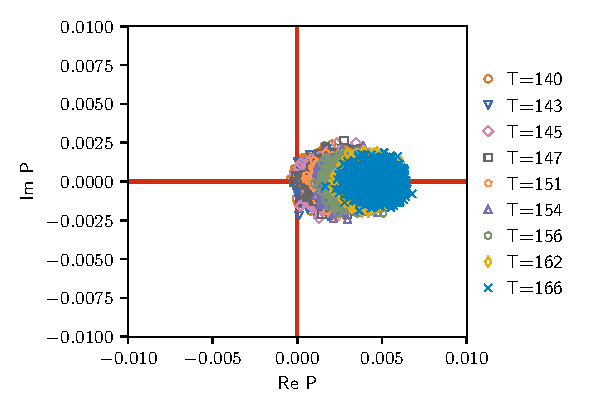
\includegraphics[width=0.8\textwidth]
          {figs/ploopScatter_betaDependl568ms80.pdf}
  \caption{Scatter plot of $P$ values for $56^3\times8$ HISQ configurations
           with $N_f=2+1$ at $m_s/m_l=80$. Temperatures are listed in MeV. 
           The real sector is preferred at finite quark mass.}
  \label{fig:ploopScatter}
\end{figure}

Let us discuss the large $N_\sigma$ behavior of some other quantities.
To simplify the notation a little, we introduce
\begin{equation}
x\equiv \Re P,~~~~y\equiv \Im P,~~~~\text{and}~~~~V\equiv N_\sigma^3.
\end{equation}
From the above discussion we have in this notation $\ev{y}=0$.
Note that $\ev{y^2}$ is generally not zero,
although it vanishes as $1/V$ with increasing V.
One can see $\ev{y^2}\neq0$ in Fig.~\ref{fig:ploopScatter}.

In particular one expects that $\ev{y^2}$ scales as
$1/V$. This is because in general $\log Z$ is proportional
to the free energy, so it is extensive and therefore scales as $V$;
therefore cumulants of extensive observables, which are coefficients in
the cumulant expansion, scale as $V$. It follows that the
susceptibility of an {\it intensive} observable scales as $1/V$,
and hence
\begin{equation}\label{eq:fssim}
  \ev{y^2}-\ev{y}^2 =\ev{y^2}=\frac{A}{V}
\end{equation}
for some volume-independent constant $A$. Indeed Fig.~\ref{fig:ImPvol} shows 
$\ev{y^2}$ scales linearly with $1/V$.

\begin{figure}
  \centering
  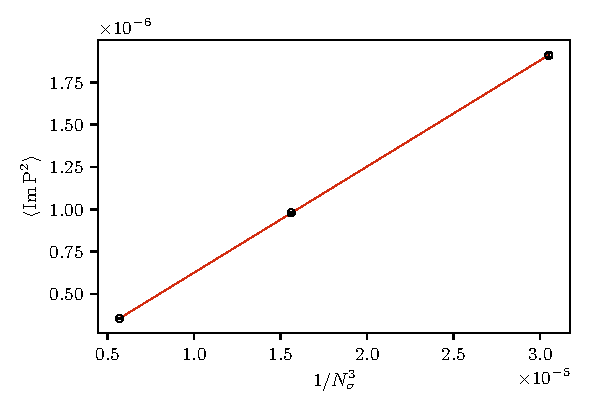
\includegraphics[width=0.8\textwidth]{figs/ImP2_voldepend.pdf}
  \caption{Volume dependence of the bare $\ev{(\Im P)^2}$ on $N_\tau=8$
           lattices with $\beta=6.445$, $m_s/m_l=80$, and $N_\sigma=32$, 40,
           and 56. The linear fit has
           $\chi^2/\text{d.o.f.}=0.11$.}
  \label{fig:ImPvol}
\end{figure}

It also follows from the scaling of terms in the cumulant expansion that
\begin{equation}\label{eq:fssre}
  \ev{x^2}-\ev{x}^2=\frac{B}{V}~~~~\text{and}~~~~\ev{x}=C
\end{equation}
for some volume-independent constants $B$ and $C$. By combining the two
equations in~\equatref{eq:fssre} one sees
\begin{equation}
  \ev{x^2}=C^2+\frac{B}{V}.
\end{equation}
In Figure~\ref{fig:FSSScalingOfSuscs} some of these relations are seen
to hold on $N_f=2+1$ HISQ lattices both above and below the chiral crossover.
We also see in this figure that $\ev{|P|}$ does not scale with volume 
in the same way as $\ev{\Re P}$ or $\ev{\Im P}$. This makes sense because
extensive quantities should scale linearly with the system size, but
absolute values are not linear. 

\begin{figure}
  \centering
  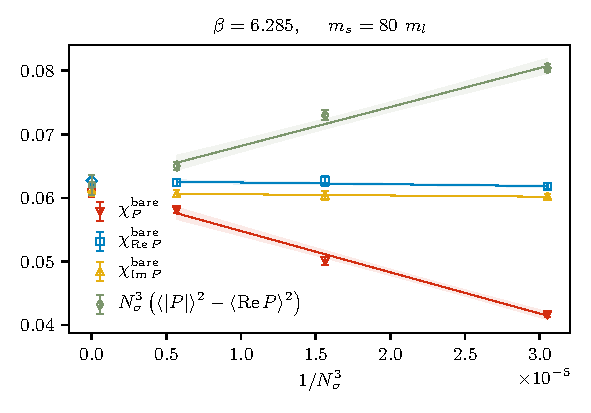
\includegraphics[width=0.45\textwidth]{figs/allSuscs_b6285.pdf}
  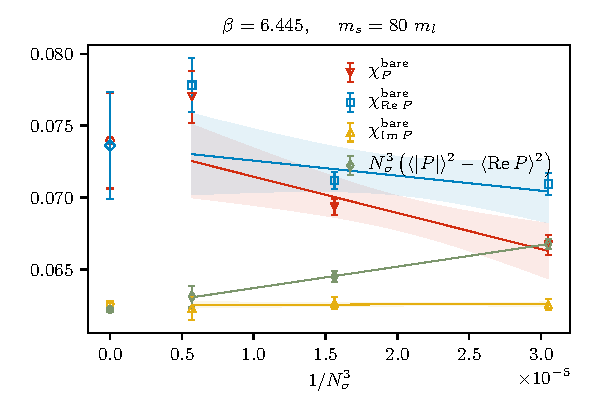
\includegraphics[width=0.45\textwidth]{figs/allSuscs_b6445.pdf}
  \caption{Finite size scaling of various susceptibilities
           for $N_\tau=8$, $m_s/m_l=80$ lattices for
           $\beta=6.285$ (left) and $\beta=6.445$ (right). Also shown are
           linear fits in $1/N_\sigma^3$ along with the
           infinite volume extrapolations.}
  \label{fig:FSSScalingOfSuscs}
\end{figure}
\bibliographystyle{unsrtnat}
\bibliography{bibliography}

\chapter{LFT: Lattice with Fermions}\label{ch:ferm}

We will now introduce Fermions on the lattice. Parts of this presentation 
follows Chapters 5 and 10 of~\cite{gattringer_quantum_2010}. 
We will start in the continuum
and introduce a naive discretization. Then we will go into detail, point
out a problem with the naive discretization, and fix it. We will omit
space-time dependence sometimes for the sake of brevity, but it should
be clear which objects have space-time dependence anyway. Primarily
we are interested in studying QCD, so $N_c=3$. This chapter uses Dirac
algebra extensively, but the algebra is different when the metric
is Euclidean. For details see \apref{ap:spec_math}.

In the continuum theory, the free fermion action is 
\begin{equation}
  S_F=\int\dd[4]{x}\bar{\psi}(\slashed{\partial}+m)\psi.
\end{equation}
Using the rules~\eqref{eq:dertodiff} and \eqref{eq:inttosum}, one naively
discretizes this action on the lattice as
\begin{equation}\label{eq:naivefermact}
  S_F=a^4\sum_x\bar{\psi}(x)\left(\sum_{\mu=1}^4\gamma_\mu
       \frac{\psi(x+a\hat{\mu})-\psi(x-a\hat{\mu})}{2a}
       +m\psi(x)\right).
\end{equation}
The fermionic partition function is
\begin{equation}
  Z_F=\int\DD{\psi}\DD{\bar{\psi}}e^{-S_F},
\end{equation}
with integration measure
\begin{equation}
  \int\DD{\psi}\DD{\bar{\psi}}
   =\prod_{x,f,\alpha,c}\dd{\bar{\psi}^f_{\alpha c}(x)}
                        \dd{\psi^f_{\alpha c}(x)},
\end{equation}
where $f$ runs over flavors, $\alpha$ runs over Dirac indices, and $c$
runs over colors.\footnote{We will try in this book to follow the convention of
Ref.~\cite{gattringer_quantum_2010} and indicate Dirac indices with Greek
letters and color indices with Latin letters.}

In addition, we want the fermionic action to be gauge invariant. The
gauge transformation for fermion fields
\begin{equation}
  \psi(x)\to U(x)\psi(x),~~~~~\bar{\psi}(x)\to\bar{\psi}(x)U(x)^\dagger
\end{equation}
with $U\in\SU(3)$ reminds us of the gauge transformation for scalar 
fields given in Chapter~\ref{ch:preliminaries}. Working in the continuum 
we introduce, just as before, a gauge field $A_\mu(x)$ so that the 
fermionic action becomes
\begin{equation}
  S_F=\int\dd[4]{x}\bar{\psi}\big(\gamma_\mu(\partial_\mu+A_\mu)+m\big)\psi.
\end{equation}
The gauge-transformed fermionic action is
\begin{equation}
  S'_F=\int\dd[4]{x}\bar{\psi}\,U^\dagger
        \big(\gamma_\mu(\partial_\mu+A'_\mu)+m\big)U\psi,
\end{equation}
so that the requirement of gauge invariance leads us to conclude
\begin{equation}
  (\partial_\mu+A_\mu)\psi=U^\dagger(\partial_\mu+A'_\mu)U\psi.
\end{equation}
Solving for $A'_\mu$ we find
\begin{equation}
  A'_\mu=(\partial_\mu U)U^\dagger-UA_\mu U^\dagger,
\end{equation}
just as with the pure gauge case. 

On the lattice, link variables transform as
\begin{equation}
  U_\mu(x)\to U'_\mu(x)=U(x)U_\mu(x)U^\dagger(x+a\hat{\mu}),
\end{equation}
which ensures that closed loops of link variables are gauge invariant.
In addition the discretized fermionic action becomes gauge invariant
when it is written as
\begin{equation}\label{eq:naivefermactgauge}
  S_F=a^4\sum_x\bar{\psi}(x)\left(\sum_{\mu=1}^4\gamma_\mu
       \frac{U_\mu(x)\psi(x+a\hat{\mu})-U_{-\mu}(x)\psi(x-a\hat{\mu})}{2a}
       +m\psi(x)\right),
\end{equation}
where
\begin{equation}
  U_{-\mu}(x)=U_\mu(x-a\hat{\mu})^\dagger
\end{equation}
transforms as
\begin{equation}
  U_{-\mu}(x)\to U'_{-\mu}(x)=U(x)U_{-\mu}(x)U^\dagger(x-a\hat{\mu}).
\end{equation}
Since \equatref{eq:naivefermactgauge} is the gauge-invariant action,
this will be what we investigate for fermion doubling.

In this chapter, it will be convenient to separate out fermionic and gluonic
parts of the path integral. To this end, we factorize expectation values as
\begin{equation}\label{eq:evfact}
\ev{...}=\ev{\ev{...}_F}_G.
\end{equation} 
For an observable $X$, the fermionic expectation value is defined as
\begin{equation}\label{eq:evferm}
\ev{X}_F\equiv\frac{1}{Z_F(U)}\int\DD\psi\DD\bar\psi
e^{-S_F\left(\bar\psi,\psi,U\right)} X\left(\bar\psi,\psi,U\right),~~~~~
Z_F(U)=\int\DD\psi\DD\bar\psi e^{-S_F\left(\bar\psi,\psi,U\right)}.
\end{equation}
This expectation value thus integrates out the fermionic degrees of freedom,
leaving only a dependence on the gauge field.
With this definition, the gluonic expectation value must be
\begin{equation}
\ev{X}_G\equiv\frac{1}{Z}\int\DD U e^{-S_G} Z_F(U) X(U)
\end{equation}
so that
\begin{equation}
\ev{X}=\frac{1}{Z}\int\DD U\DD\psi\DD\bar\psi
e^{-S_G(U)-S_F\left(\bar\psi,\psi,U\right)} X\left(\bar\psi,\psi,U\right)
\end{equation}
as expected.

\section{Grassmann numbers}\label{sec:grassmann}\index{algebra!Grassmann}
\index{Grassmann!algebra}
Fermions are objects that by definition anticommute with each other. 
With this in mind, we introduce Grassmann numbers.
We consider a set of numbers $\eta_i$, $1\leq i\leq N$ obeying
\begin{equation}
  \eta_i\eta_j=-\eta_j\eta_i
\end{equation}
for all $i$ and $j$. These are called {\it Grassmann
numbers}\index{Grassmann!number}.
It follows that
\begin{equation}\label{eq:gnilpotent}
  \eta_i^2=0.
\end{equation}
If a power series of a function $f$ of the Grassmann numbers exists, then
\equatref{eq:gnilpotent} guarantees that the series terminates almost
immediately. In general we would write
\begin{equation}\label{eq:grasspoly}
  f(\eta)=a+\sum_ia_i\eta_i+\sum_{i<j}a_{ij}\eta_i\eta_j
           +...+a_{1...N}\eta_1...\eta_N
\end{equation}
with $a,\,a_i,\,a_{ij},...,\,a_{1...N}\in\mathbb{C}$.
We refer to \equatref{eq:grasspoly} as a {\it Grassmann polynomial}.
Grassmann\index{Grassmann!polynomial} 
polynomials are closed under addition and multiplication,
and are thus said to form a {\it Grassmann algebra}. The $\eta_i$
are the {\it generators} of the Grassmann algebra.

To learn how differentiation ought to work, we use the simple example
$N=2$. Then
\begin{equation}
  f(\eta)=a+a_1\eta_1+a_{12}\eta_1\eta_2.
\end{equation}
A definition of the derivative that follows our intuition is
\begin{equation}
  \pdv{f}{\eta_1}=a_1+a_{12}\eta_2.
\end{equation}
However, the defining characteristic of Grassmann numbers is that they
anticommute. Therefore we could also have expanded $f$ as
\begin{equation}
  f(\eta)=a+a_1\eta_1-a_{12}\eta_2\eta_1.
\end{equation}
In order for the derivative $f$ to make sense we must therefore require
\begin{equation}
  \pdv{\eta_1}\eta_2=
  -\eta_2\pdv{\eta_1}.
\end{equation}
Similarly if we take another derivative, this time with respect to $\eta_2$,
we find that partial derivatives with respect to different Grassmann variables
must also anticommute to maintain consistency. Altogether, the differentiation
rules for Grassmann variables become
\begin{equation}\begin{aligned}
  \pdv{\eta_i}1&=0;\\
  \pdv{\eta_i}\eta_i&=1;\\
  \pdv{\eta_i}\eta_j&=
  -\eta_j\pdv{\eta_i};\\
  \frac{\partial^2}{\partial\eta_i\partial\eta_j}&=
  -\frac{\partial^2}{\partial\eta_j\partial\eta_i}.
\end{aligned}\end{equation}

Next we move on to integration. We will construct integrals that work like
integrals over subsets $\Omega\in\mathbb{R}^N$ for which 
the integrand vanishes at the boundary $\partial\Omega$. 
Thus we demand that the Grassmann integral is a complex number,
\begin{equation}
  \int\dd[N]{\eta}f\in\mathbb{C};
\end{equation}
that with $\lambda_1,\lambda_2\in\mathbb{C}$ it is linear,
\begin{equation}\label{eq:grasslin}
  \int\dd[N]{\eta}\left(\lambda_1f_1+\lambda_2f_2\right)
       =\lambda_1\int\dd[N]{\eta}f_1
         +\lambda_2\int\dd[N]{\eta}f_2;
\end{equation}
and that its integrand vanishes at the boundary,
\begin{equation}\label{eq:grassBC}
  \int\dd[N]{\eta}\pdv{\eta_i}f=0.
\end{equation}
If some function $f$ of $N-1$ Grassmann numbers can be written as the 
derivative of another function $g$ of $N$ Grassmann numbers, it follows
from \equatref{eq:grassBC} that the integrand vanishes.
An integral of a Grassmann polynomial of $N$ variables is therefore
proportional to the coefficient $a_{1...N}$, since
$\eta_1...\eta_N$ cannot be written as a derivative of $N$ variables.
In particular if we demand a normalization
\begin{equation}\label{eq:grassnorm}
  \int\dd[N]{\eta}\eta_1...\eta_N=1,
\end{equation}
we obtain the rule
\begin{equation}
  \int\dd[N]{\eta}f=a_{1...N}.
\end{equation}
Finally to make Grassmann integration more analogous to the integration that
we're used to, we define
\begin{equation}
  \dd[N]{\eta}\equiv\dd{\eta_N}...\dd{\eta_1}.
\end{equation}
Altogether then, the rules of Grassmann integration can be summarized by
\equatref{eq:grasslin} along with
\begin{equation}\label{eq:grassintrules}\begin{aligned}
       \int\dd{\eta_i}1&=0;\\
  \int\dd{\eta_i}\eta_i&=1;\\
  \dd{\eta_i}\dd{\eta_j}&=-\dd{\eta_j}\dd{\eta_i}.
\end{aligned}\end{equation}
Using these properties we can define integration over subsets of Grassmann
variables. Interestingly, the measures obey the same algebraic properties as
the derivatives.

Next let us discuss how Grassmann integrals behave under linear
transformations. In general we can write such a change of variables as
\begin{equation}\label{eq:grassxform}
  \eta'_i=M_{ij}\eta_j,
\end{equation}
where $M$ is a complex $N\times N$ matrix. More succinctly, one writes 
$\eta'=M\,\eta$. Applying this change of variables to the normalization
\equatref{eq:grassnorm} we obtain
\begin{equation}\begin{aligned}
  \int\dd[N]{\eta}\eta_1...\eta_N
     &=1\\
     &=\int\dd[N]{\eta'}\eta'_1...\eta'_N\\
     &=\int\dd[N]{\eta'}M_{1\,i_1}...M_{N\,i_N}\,\eta_{i_1}...\eta_{i_N}\\
     &=\int\dd[N]{\eta'}M_{1\,i_1}...M_{N\,i_N}\,\epsilon_{i_1...i_N}
               \eta_1...\eta_N\\
     &=\int\dd[N]{\eta'}\det M\,\eta_1...\eta_N.
\end{aligned}\end{equation}
It follows that under the transformation~\eqref{eq:grassxform}, the measure
transforms according to the rule
\begin{equation}
  \dd[N]{\eta}=\det M\dd[N]{\eta'},
\end{equation}
which is in some sense the ``opposite" of the usual transformation rule, where
the $\det M$ would have been on the LHS.

The stuff between the parentheses in the naive action~\eqref{eq:naivefermact}
can be viewed as an operator. Keeping this in mind, we're going to show
that the fermionic partition function can be viewed as a determinant.
The setup is as follows: We have a Grassmann algebra with $2N$ generators
$\bar{\eta}_i$ and $\eta_i$ that all anticommute with each other and
an $N\times N$ linear transformation $M$.
\begin{theorem}{Matthews-Salam formula}{}
\index{Matthews-Salam formula}
$$
  \int\prod_{i=1}^N\dd{\eta_i}\dd{\bar{\eta}_i}e^{\bar{\eta}M\eta}=\det M.
$$
\begin{proof} Let $\eta'=M\eta$. Then from \equatref{eq:grassxform}
  we have
  \begin{equation*}\begin{aligned}
  \int \prod_{i=1}^N\dd{\eta_i}\dd{\bar{\eta}_i}e^{\bar{\eta}M\eta}
    &=\det M\int \prod_{i=1}^N\dd{\eta'_i}\dd{\bar{\eta}_i}
       \exp\left(\sum_{j=1}^N\bar{\eta}_j\eta'_j\right)\\
    &=\det M\int \prod_{i=1}^N\dd{\eta'_i}\dd{\bar{\eta}_i}
       \exp\left(\bar{\eta}_i\eta'_i\right)\\
    &=\det M\int \prod_{i=1}^N\dd{\eta'_i}\dd{\bar{\eta}_i}
        (1+\bar{\eta}_i\eta'_i)\\
    &=\det M.
  \end{aligned}\end{equation*}
  The second line follows since pairs $\bar{\eta}_i\eta_i$ commute with
  each other, the third line is a power series expansion of the second
  line, and the last line follows from \equatref{eq:grassintrules}.
\end{proof}
\end{theorem}

Let us take a moment to see how the Matthews-Salam formula is employed
in lattice field theory. In our case, our Grassman variables are
fermion fields. The integration measure is a product over all
space-time sites, so that the index $i$ labels the site.
The matrix that occurs for us is the 
{\it Dirac operator}\index{Dirac!operator}
or {\it Dirac matrix}\index{Dirac!matrix} $D(x,y)$, appearing
in the action like
\begin{equation}\label{eq:diracPositionBasis}
\bar{\psi}(x)\left(\slashed{D}+m\right)\psi(y)
\equiv\bar{\psi}(x)D(x,y)\psi(y).
\end{equation}
Remember that $\slashed{D}$ contains a covariant derivative, which
is responsible for parallel transport between $x$ and its neighbors,
which is why we write $D(x,y)$. When we write $D(x,y)$, we are
now thinking about $\slashed{D}+m$ as a matrix in the basis
of spacetime points. The form of $D(x,y)$ will depend on how we
discretize\footnote{For example the Wilson action, which we will discuss
in \secref{sec:LFTdoubling}, has Kronecker $\delta$-functions that
enforce each site only interacts with its immediate neighbors.
In that sense the Wilson Dirac operator is ``tridiagonal".
The HISQ action on the other hand, which we will discuss in 
\secref{sec:HISQ}, includes interactions between sites and
their next-to-nearest neighbors. This is analogous to having a 
band diagonal matrix.}. Hence Matthews-Salam will let us trade
away the fermion fields for the determinant of the Dirac operator.
Due to the incredible size of $D(x,y)$, computing its determinant
is prohibitively computationally expensive. We will discuss the most
commonly used trick to avoid this in \secref{sec:pseudofermions}.

If we replace $M$ with the Dirac operator, we see that the fermionic
partition function is just the determinant of the Dirac operator.
By the way, the ordering of the differentials in the measure should
be $\dd{\eta}\dd{\bar{\eta}}$. This is because the $\bar{\eta}$ variables
in the integrand will always come on the left. By placing the
$\dd{\bar{\eta}}$ differentials on the right, it will always hit the
$\bar{\eta}$ variables first.

A generalization of this gives us the generating functional
for fermions. Here we consider $4N$ Grassmann numbers $\bar{\eta}_i$,
$\eta_i$, $\bar{\theta}_i$, and $\theta_i$. The $\bar{\theta}_i$
and the $\theta_i$ are the source terms. We define
\begin{equation}\label{eq:deffermgf}
  W[\theta,\bar{\theta}]\equiv\int \prod_{i=1}^N\dd{\bar{\eta}_i}\dd{\eta_i}
   e^{\bar{\eta}M\eta+\bar{\theta}\eta+\bar{\eta}\theta}
\end{equation}
\begin{theorem}{}{fermgf}
$$
   W[\theta,\bar{\theta}]=e^{-\bar{\theta}M^{-1}\theta}\det M.
$$
\begin{proof} Using the definition of the generating functional and
completing the square, we have 
$$
  \int \prod_{i=1}^N\dd{\bar{\eta}_i}\dd{\eta_i}
   e^{\bar{\eta}M\eta+\bar{\theta}\eta+\bar{\eta}\theta}
   =\int \prod_{i=1}^N\dd{\bar{\eta}_i}\dd{\eta_i}
   e^{(\bar{\eta}+\bar{\theta}M^{-1})\,M\,
             (\eta+M^{-1}\theta)-\bar{\theta}M^{-1}\theta}.
$$
Now we define new variables $\bar{\eta}'=\bar{\eta}+\bar{\theta}M^{-1}$
and $\eta'=\eta+M^{-1}\theta$. From \equatref{eq:grassintrules} it follows
that
$$
  \int \prod_{i=1}^N\dd{\bar{\eta}_i}\dd{\eta_i}=
  \int \prod_{i=1}^N\dd{\bar{\eta}'_i}\dd{\eta'_i}.
$$
Therefore by the Matthews-Salam formula,
\begin{equation*}\begin{aligned}
   \int \prod_{i=1}^N\dd{\bar{\eta}_i}\dd{\eta_i}
   e^{(\bar{\eta}+\bar{\theta}M^{-1})\,M\,
             (\eta+M^{-1}\theta)-\bar{\theta}M^{-1}\theta}
   &=\int \prod_{i=1}^N\dd{\bar{\eta}'_i}\dd{\eta'_i}
    e^{\bar{\eta}'M\eta'-\bar{\theta}M^{-1}\theta}\\
   &=e^{-\bar{\theta}M^{-1}\theta}\det M.
\end{aligned}\end{equation*}
\end{proof}
\end{theorem}
With the knowledge we now have, we can derive Wick's theorem, which lets us
calculate fermionic expectation values. First we define 
\begin{equation}\label{eq:deffermev}
  \ev{\eta_{i_1}\bar{\eta}_{j_1}...\eta_{i_n}\bar{\eta}_{j_n}}_F
  \equiv\frac{1}{Z_F}\int\prod_{k=1}^N\dd{\eta_k}\dd{\bar{\eta}_k}
        \bar{\eta}_{j_1}...\eta_{i_n}\bar{\eta}_{j_n}
        e^{-\bar{\eta}M\eta}.
\end{equation}
\begin{theorem}{Wick's theorem}{}
\index{Wick's theorem}
$$
  \ev{\eta_{i_1}\bar{\eta}_{j_1}...\eta_{i_n}\bar{\eta}_{j_n}}_F
  =(-1)^n\sum_{P_{1,...,n}}\sign P\,
   M^{-1}_{i_1,j_{P_1}}\,...\,M^{-1}_{i_n,j_{P_n}}.
$$
\begin{proof} From the definitions~\eqref{eq:deffermgf} and
  \eqref{eq:deffermev} we have
  $$
    \ev{\eta_{i_1}\bar{\eta}_{j_1}...\eta_{i_n}\bar{\eta}_{j_n}}_F
    =\frac{1}{Z_F}
    \pdv{\theta_{j_1}}
    \pdv{\bar{\theta}_{i_1}}\,...\,
    \pdv{\theta_{j_n}}
    \pdv{\bar{\theta}_{i_n}}W[\theta,\bar{\theta}]
    \Big|_{\theta=\bar{\theta}=0}.
  $$
  Let us now apply Theorem~\ref{thm:fermgf} to the RHS and carry
  out the derivatives. The $\det M$ will cancel with $Z_F$ because
  of the Matthews-Salam formula. 
\end{proof}
\end{theorem}

\section{Fermion doubling}\label{sec:LFTdoubling}
Let us now discuss one of the important problems with the naive fermionic
action. First we introduce some results about Fourier transformations on the
lattice. Define
\begin{equation}
V\equiv N_1N_2N_3N_4
\end{equation}
with $N_\mu$ even.\index{BCs!toroidal}
We generalize to {\it toroidal BCs}, i.e.
\begin{equation}
  f(x+aN_\mu\hat{\mu})=e^{2\pi i\theta_\mu}f(x).
\end{equation}
Periodic BCs then have $\theta_\mu=0$ and {\it anti-periodic BCs} have
\index{BCs!anti-periodic}
$\theta_\mu=1/2$. The momentum space becomes
\begin{equation}
  p_\mu=\frac{2\pi}{aN_\mu}(k_\mu+\theta_\mu),~~~~~~
   -\frac{N_\mu}{2}<k_\mu\leq\frac{N_\mu}{2},
\end{equation}
which reduces to the first Brillouin zone when periodic BCs are employed. By
including the boundary phases in the momentum definition, plane waves
\begin{equation}
  \exp(ip_\mu x_\mu)
\end{equation}
will also obey the BCs. Now we derive a basic formula for Fourier
transformations on the lattice. Let $N$ be even and $\ell$ be an integer
$0\leq\ell\leq N-1$.
\begin{proposition}{}{}
$$
  \frac{1}{N}\sum_{j=-N/2+1}^{N/2}\exp(\frac{2\pi i\ell}{N})^j=\delta_{\ell 0}.
$$
\begin{proof} Since $N$ is even there are $N$ terms in the above sum,
  so we find the LHS to be 1. For $\ell\neq 0$ let
  $m\equiv j+N/2+1$ and define
  $$
    q\equiv\exp(\frac{2\pi i\ell}{N}).
  $$
  Then
  \begin{equation*}\begin{aligned}
    \frac{1}{N}\sum_{j=-N/2+1}^{N/2}\exp(\frac{2\pi i\ell}{N})
      \propto\sum_{m=0}^{N-1}q^m
      =\frac{1-q^N}{1-q}=0
  \end{aligned}\end{equation*}
  since $q^N=1$.
\end{proof}
\end{proposition}
Applying this formula in each space-time direction, we arrive at
\begin{equation}
  \frac{1}{V}\sum_p\exp\big(ip_\mu(x-x')_\mu\big)
  =\delta(x-x')
  =\delta_{n_1n'_1}\delta_{n_2n'_2}\delta_{n_3n'_3}\delta_{n_4n'_4},
\end{equation}
where $x_\mu=an_\mu$, and
\begin{equation}
  \frac{1}{V}\sum_x\exp\big(i(p-p')_\mu x_\mu\big)
  =\delta(p-p')
  =\delta_{k_1k'_1}\delta_{k_2k'_2}\delta_{k_3k'_3}\delta_{k_4k'_4}.
\end{equation}
We define the Fourier transform as
\begin{equation}\label{eq:latft}
  \tilde{f}(p)=\frac{1}{\sqrt{V}}\sum_xf(x)\exp(-ip_\mu x_\mu).
\end{equation}
The inverse transform
\begin{equation}\label{eq:latift}
  f(x)=\frac{1}{\sqrt{V}}\sum_p\tilde{f}(p)\exp(ip_\mu x_\mu)
\end{equation}
can be verified by plugging the Fourier transform into the LHS.

Using these results about Fourier transformations on the lattice, we
can begin to investigate fermion doubling. We shall do this for
a single flavor for notational convenience; the result clearly
generalizes to a summation over flavors. 
The gauge-invariant, naive
fermion action~\eqref{eq:naivefermactgauge} is bilinear in $\psi$
and $\bar{\psi}$, so it can be written as
\begin{equation}
  S_F=a^4\sum_{x,y}\sum_{\alpha,\beta,c_1,c_2}\bar{\psi}(x)_{\alpha c_1}
      \,D(x,y)_{\alpha \beta c_1 c_2}\,\psi(y)_{\beta c_2},
\end{equation}
where $\alpha$ and $\beta$ are Dirac indices, $c_1$ and $c_2$ are
color indices, and the Dirac operator on the lattice is
\begin{equation}
  D(x,y)_{\alpha\beta c_1c_2}\equiv\sum_{\mu=1}^4(\gamma_\mu)_{\alpha\beta}
   \frac{U_\mu(x)_{c_1c_2}\delta_{x+a\hat{\mu},y}
         -U_{-\mu}(x)_{c_1c_2}\delta_{x-a\hat{\mu},y}}{2a}
   +m\delta_{\alpha\beta}\delta_{c_1c_2}\delta_{xy}.
\end{equation}
In this form, we can apply the Matthews-Salam formula or Wick's
theorem by identifying $M=a^4D$. 

For simplicity, we set $U_\mu(x)=\id$
for all links, just so we can see clearly how the doubling arises.
Since we have free fermions, we may as well suppress color indices,
and we will also use vector/matrix notation in Dirac space, so that
Dirac indices are also suppressed. We find
\begin{equation}\begin{aligned}
  \tilde{D}(p,q)&=\frac{1}{V}\sum_{x,y}e^{-ipx}D(x,y)e^{-iqy}\\
     &=\frac{1}{V}\sum_{x,y}e^{-ipx}\left(
      \sum_\mu\gamma_\mu\frac{\delta_{x+a\hat{\mu},y}
                             -\delta_{x-a\hat{\mu},y}}{2a}+m\delta_{x,y}\id
      \right)e^{-iqy}\\
     &=\frac{1}{V}\sum_xe^{-i(p+q)x}\left(
      \sum_\mu\gamma_\mu\frac{e^{iq_\mu a}-e^{-iq_\mu a}}{2a}+m\id\right)\\
     &=\delta(p+q)\left(\frac{i}{a}\sum_\mu
                    \gamma_\mu\sin(q_\mu a)+m\id\right)\\
     &\equiv\delta(p+q)\tilde{D}(q).
\end{aligned}\end{equation}
In Ref.~\cite{gattringer_quantum_2010} they take the transform
of the $y$ part to have opposite sign, which they say makes the similarity
transformation unitary. For the purpose of seeing fermion doubling
the sign does not make a difference; it only changes the delta
function from $\delta(p-q)$ to $\delta(p+q)$. Therefore I decided to stick
with the convention~\eqref{eq:latft}. If we want to use Wick's theorem,
we will need to calculate the inverse of the Dirac operator. We find
\begin{equation}\label{eq:latprop}
  \tilde{D}(p)^{-1}=\frac{m\id-ia^{-1}\sum_\mu\gamma_\mu\sin(p_\mu a)}
                         {m^2+a^{-2}\sum_\mu\sin(p_\mu a)^2},
\end{equation}
which can be verified by multiplying both sides by $\tilde{D}(p)$. This
is the propagator for free fermions in momentum space. At $m=0$ we find
as $a\to0$
\begin{equation}
  \tilde{D}(p)^{-1}\to\frac{-i\sum_\mu\gamma_\mu p_\mu}{p^2}.
\end{equation}
This propagator has a pole at $p=0$. Poles in propagators correspond
to physical particles, so in the continuum theory, the propagator
corresponds to a single particle satisfying the Dirac equation. On
the lattice if the fermions are massless, \equatref{eq:latprop} has
a pole anywhere $p_\mu a=\pi$. In the first Brillouin zone, this
happens 15 places besides $p_\mu=0$. Hence on the lattice at finite
spacing, the propagator has 15 unphysical poles that nevertheless
correspond to some fermions. This is called {\it fermion doubling},
\index{fermion!doubling}
and we call the 15 unwanted particles the {\it doublers}.

This proliferation of extra particles can cause problems in the
interacting theory. The additional states can be pair produced
through interactions of the fermion field~\cite{montvay_quantum_1994}.
For instance even if all particles on the external lines of a diagram
are the real particles, the doublers can appear in virtual loops.
Therefore one typically wants to remove the doublers.

One way to remove the doublers is to introduce an extra term that
cancels the doublers on the lattice, and still reduces to the
correct continuum value. With this formulation, the lattice
momentum space Dirac operator is
\begin{equation}
  \tilde{D}(p)=m\id+\frac{i}{a}\sum_\mu\gamma_\mu\sin(p_\mu a)
                   +\frac{1}{a}\sum_\mu\id\big(1-\cos(p_\mu a)\big).
\end{equation} 
This second term is called the {\it Wilson!term}. This formulation
\index{fermion!Wilson}\index{Wilson!fermions}
of fermions is called {\it Wilson fermions}. The complete Dirac
operator using this formulation becomes 
\begin{equation}
  D(x,y)^f_{\alpha\beta c_1c_2}
  =\left(m^f+\frac{4}{a}\right)\delta_{\alpha\beta}
                               \delta_{c_1c_2}
                               \delta_{xy}
   -\frac{1}{2a}\sum_{\mu=\pm 1}^{\pm 4}(\id-\gamma_\mu)_{\alpha\beta}
      U_\mu(x)_{c_1 c_2}\delta_{x+a\hat{\mu},y},
\end{equation}
where
\begin{equation}
  \gamma_{-\mu}\equiv-\gamma_{\mu}.
\end{equation}

\section{Staggered
fermions}\index{fermion!staggered}\index{staggered!fermions}\label{sec:stagg}

In this section we work in a free theory to simplify the notation.
In the interacting theory, each spinor will have a link attached to it
originating at the same point, and the Dirac indices that we will
manipulate commute with these links, so the derivation will be the same.
This follows parts of Section 10.1 of Ref.~\cite{gattringer_quantum_2010} 
and Section 4.4 in Ref.~\cite{rothe_lattice_2005}.
If you would like to take a deeper look at staggered fermions,
Ref.~\cite{Golterman:2024xos} gives a comprehensive review.

In \secref{sec:LFTdoubling} we saw that the doubling problem could
be alleviated by adding a Wilson term of the form
\begin{equation}
  \frac{1}{a}\sum_\mu\id\big(1-\cos(p_\mu a)\big).
\end{equation}
Writing this as exponentials, and doing the Fourier back transformation,
we can express this as
\begin{equation}
  a\sum_{\mu=1}^4\frac{1}{2a^2}
\left(2\delta_{x,y}-\delta_{x,y-a\hat{\mu}}-\delta_{x,y+a\hat{\mu}}\right).
\end{equation}
In this form, one clearly sees that the Wilson term vanishes in the
naive continuum limit like $a$. Moreover it has the form of a
discretized $\partial_\mu\partial_\mu$. A drawback of this term,
however, is that it breaks $\SU_A(N_f)\times\U_A(1)$ explicitly
because the Wilson term commutes with $\gamma_5$.

For some calculations one may desire not to break this symmetry entirely,
in particular when one is investigating phenomena closely related to
chiral symmetry. This motivates other possible fermion discretizations
that remove doublers. {\it Staggered fermions} will remove some of the 
unphysical doublers, while keeping a remnant of this axial symmetry intact. 
This is accomplished by redistributing the quark degrees of freedom over
the lattice in such a way that the spacing between each degree of freedom
doubles, thereby doubling the effective lattice spacing, and hence
reducing the size of the Brillouin zone. New quarks called {\it tastes}\index{taste}
will be constructed by linear combinations of these degrees of freedom.

We take as the starting point the naive fermion action
\begin{equation}
 S_F
     =a^4\sum_n\bar{\psi}(n)\left(\sum_{\mu=1}^4\gamma_\mu
       \frac{\psi(n+\hat{\mu})-\psi(n-\hat{\mu})}{2a}
       +m\psi(n)\right).
\end{equation}
In this equation and in what follows I will write the space-time coordinate
as $n$ to make the connection between the space-time coordinate and the
following more clear. The {\it staggered
transformation}\index{staggered!transformation} is given by
\begin{equation}\begin{aligned}
\psi(n)&=\gamma_1^{n_1}\gamma_2^{n_2}\gamma_3^{n_3}\gamma_4^{n_4}\psi(n)'\\
\bar{\psi}(n)
   &=\bar{\psi}(n)'\gamma_4^{n_4}\gamma_3^{n_3}\gamma_2^{n_2}\gamma_1^{n_1}
\end{aligned}\end{equation}

The fact that these transformed fields come with power of gamma matrices,
along with the fact that $\gamma_\mu^2=\id$, will
diagonalize the naive action in Dirac space. In particular one finds
relationships such as
\begin{equation}
  \bar{\psi}(n)\gamma_4\psi(n+\hat{4})
      =(-1)^{n_1+n_2+n_3}\bar{\psi}(n)'\id\psi(n+\hat{4}),
\end{equation}
which means that in the kinetic part, the gamma matrices are annihilated,
and what remains are scalar {\it staggered phases}\index{staggered!phase}
\begin{equation}\label{eq:staggeredPhase}
   \eta_1(n)=1, ~~~
   \eta_2(n)=(-1)^{n_1}, ~~~
   ...\,, ~~~
   \eta_4(n)=(-1)^{n_1+n_2+n_3}.
\end{equation}
Substituting the staggered fields
into the naive action, we thus find
\begin{equation}\label{eq:SFdiag}
   S_F
     =a^4\sum_n\bar{\psi}(n)'\id\left(\sum_{\mu=1}^4\eta_\mu(n)
       \frac{\psi(n+\hat{\mu})'-\psi(n-\hat{\mu})'}{2a}
       +m\psi(n)'\right),
\end{equation}
which is now diagonal in Dirac space because the gammas are gone.
The Dirac operator of \equatref{eq:SFdiag} represents four copies of
the same equations along its diagonal, so we can throw away three copies
without losing any information. We will call this last, kept copy $\chi$;
another way of looking at this is we keep only one Dirac component.
With this notation, we find a particularly simple form for the staggered
action:
\begin{equation}\label{eq:stagg1}
  S_F^{\rm stag}
     =a^4\sum_n\bar{\chi}(n)\left(\sum_{\mu=1}^4\eta_\mu(n)
       \frac{\chi(n+\hat{\mu})-\chi(n-\hat{\mu})}{2a}
       +m\chi(n)\right)
\end{equation}

Equation \eqref{eq:stagg1} is convenient for simulations because it contains no
Dirac spinors explicitly, but we would like a form that tells us a little
more about the physics. We will now begin to rewrite this equation in such
a way that we see the increase of the effective lattice spacing. The
strategy will be to divide the lattice into disjoint unit hypercubes.
The $\chi$ live on the corners of the hypercubes. New fields $q$ will be 
linear combination of the $\chi$, and their sites will be indexed by 
hypercube number.

To this end, we introduce new vectors $h$ (hypercube) and $s$ (corner) that
are related to the original site vectors by
\begin{equation}\label{eq:hypercubeIndex}
  n_\mu=2h_\mu+s_\mu~~~\text{with}~~~h_\mu\in\{0, 1, ..., N_\mu/2\}
                    ~~~s_\mu\in\{0,1\}.
\end{equation}
Moving in the direction $\mu$, $h_\mu$ counts the hypercube number,
while $s$ is a displacement vector starting at the hypercube's origin.
In this indexing scheme
\begin{equation}
  \eta_\mu(n)=\eta_\mu(2h+s)=\eta_\mu(s)
\end{equation}
because contributions to powers of gamma coming from the hypercubes are
always even, according to \equatref{eq:hypercubeIndex}.

Next we introduce $\Gamma$, which will serve as the weights in the linear
combination. We define
\begin{equation}
  \Gamma^s=\gamma_1^{s_1}\gamma_2^{s_2}\gamma_3^{s_3}\gamma_4^{s_4}.
\end{equation}
These obey, respectively, orthogonality and completeness 
relations\footnote{The orthogonality relation can be proven using
properties of the Euclidean $\gamma$ matrix, in particular that
$\gamma_\mu=\gamma_\mu^\dagger=\gamma_\mu^{-1}$.} 
\begin{equation}
\frac{1}{4}\tr\left[\Gamma^{s\dagger}\Gamma^{s'}\right]=\delta_{ss'}
~~~~\text{and}~~~~
\frac{1}{4}\sum_s\Gamma_{ba}^{s*}\Gamma_{b'a'}^s=\delta_{aa'}\delta_{bb'}
\end{equation}
Our new quark fields are then (see \figref{fig:staggHypercubes})
\begin{equation}\label{eq:staggqdef}
  q(h)_{ab}\equiv\frac{1}{8}\sum_s\Gamma^s_{ab}\chi(2h+s)
~~~~\text{and}~~~~
  \bar{q}(h)_{ab}\equiv\frac{1}{8}\sum_s\bar{\chi}(2h+s)\Gamma^{s*}_{ab}.
\end{equation}
In order to cast the staggered action in terms of $q(h)$, we need to
invert \equatref{eq:staggqdef}. This can be done using the
orthogonality relation. One obtains
\begin{equation}
  \chi(2h+s)=2\tr\left[\Gamma^{s\dagger}q(h)\right]
  ~~~~\text{and}~~~~
  \bar{\chi}(2h+s)=2\tr\Big[\bar{q}(h)\Gamma^s\Big].
\end{equation}

\begin{figure}[t]
  \centering
  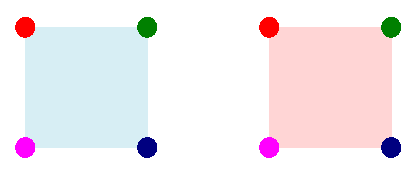
\includegraphics{figs/staggHypercubes.pdf}
  \caption{Example subdivision of one direction into disjoint hypercubes.
           Each hypercube is labeled by $h$, and the field $q(h)$
           associated to the hypercube is a linear combination of the
           $\chi$ fields on the corners, here represented by
           different colors. The effective lattice spacing between
           a $\chi$ of one corner of the blue hypercube and the corresponding
           $\chi$ in the same corner of the red hypercube is $a'=2a$.
           }
  \label{fig:staggHypercubes}
\end{figure}

We are now ready to carry out the substitution. The mass term follows
straightforwardly from the completeness relation. The kinetic term is
difficult, however, because the site offsets mix hypercubes. Therefore
it is crucially important to keep track of which hypercube $\chi$
belongs to. Keeping track of the hypercube will make manifest an $s$
dependence that makes applying the completeness relation not possible,
at least superficially. Gattringer and Lang~\cite{gattringer_quantum_2010}
suggest the following trick: we can shift the site that the first
hypercube starts on by one, which gives equivalent results as the
original hypercube labeling convention, and then average over these
two conventions. I was not able to figure this out. 
Rothe~\cite{rothe_lattice_2005} has another strategy, which I was also
not able to follow through. Nevertheless, one should find
\begin{equation}
S_F^{\rm stag}=a'^4\sum_h\Big(m\tr\left[\bar{q}q\right]
+\tr\left[\bar{q}\gamma_\mu\partial_\mu q\right]
-\frac{a'}{2}\tr\left[\bar{q}\gamma_5\Box_\mu q\gamma_\mu\gamma_5\right]\Big)
\end{equation}
where we have an implied summation over $\mu$, we have written
$q=q(h)$, introduced the effective spacing $a'\equiv2a$, and 
the discretized derivatives are
\begin{equation}
  \partial_\mu f(h)\equiv\frac{f(h+\hat{\mu})-f(h-\hat{\mu})}{2a'}
\end{equation}
and
\begin{equation}
  \Box_\mu f(h)\equiv\frac{f(h+\hat{\mu})-2f(h)+f(h-\hat{\mu})}{a'^2}.
\end{equation}

Our final step in the exploration of the staggered action will be to
identify the unphysical fermions. These {\it tastes} are hidden in
\index{taste}
the $q$. This should not be surprising because the $q_{ab}$ have 16
components, but Dirac spinors should have 4. This
tells us each $q$ corresponds to 4 spinors, and we will identify from
the $a$ and $b$ a taste index and Dirac index.
By comparing e.g. the $\tr[\bar{q}q]=\bar{q}_{ab}q_{ba}$ term with
what we expect from the physical, continuum theory, it makes sense
to identify the Dirac index with $b$. Thus our taste spinors are
\begin{equation}
  \psi^{t}(h)_\alpha\equiv q(h)_{\alpha t}~~~~\text{and}~~~~
  \bar{\psi}^{t}(h)_\alpha\equiv \bar{q}(h)_{t\alpha}.
\end{equation}
The staggered fermion action then becomes
\begin{equation}\label{eq:staggPhys}
S_F^{\rm stag}=a'^4\sum_h\left(
m\bar{\psi}^{t}\psi^{t}
+\bar{\psi}^{t}\gamma_\mu\partial_\mu\psi^{t}
-\frac{a'}{2}\bar{\psi}^{t}\gamma_5(\tau_5\tau_\mu)_{tt'}\Box_\mu\psi^{t'}
\right),
\end{equation}
where we have introduced new matrices
\begin{equation}
\tau_\mu\equiv\gamma_\mu^T.
\end{equation}

With the staggered action in the form of \equatref{eq:staggPhys} we can
begin to discuss some physics. The last term is called the
\index{taste!breaking}
{\it taste-breaking} term. It is similar to the Wilson term, in the
sense that it also represents a second derivative. However unlike
the Wilson term, it allows for interactions between fermions of
\index{taste!mixing}
different taste, i.e. it allows for {\it taste mixing}. If not for
the taste-breaking term, fermions of different taste would be mass-degenerate,
which one sees clearly from the first term. In the naive continuum limit,
this taste breaking terms vanishes like $a$.

The Wilson term broke axial symmetry completely, but in the taste-breaking
term, the remnant $\U_A(1)\times\U_A(1)$ remains. In particular this
term is invariant under transformations
\begin{equation}
\psi'=e^{i\omega}\psi, ~~~~~~
          \bar{\psi}'=\bar{\psi}e^{-i\omega}
\end{equation}
and
\begin{equation}
   \psi'=e^{i\omega\gamma_5\otimes\tau_5}\psi, ~~~~~~
          \bar{\psi}'=\bar{\psi}e^{i\omega\gamma_5\otimes\tau_5}.
\end{equation}
This latter symmetry follows from the fact that $\gamma_5$ commutes through
the taste-breaking term, while $\tau_5$ will pick up a minus sign.
One can identify this symmetry with a subgroup of the axial taste
symmetry group $\SU_A(N_t)$, where $N_t$ is the number of tastes.

At finite lattice spacing, taste mixing lifts the taste mass degeneracy.
One way to get some feeling for taste-breaking effects, then, is to look
at the mass spectrum of staggered fermions. It has been found that these
taste breaking effects can be reduced by improved gauge actions or smearing
\cite{durr_staggered_2004,follana_index_2004}, and in particular smearing
seems to drive masses to 4-fold degeneracy. An intuition for why smearing
might help is as follows: In the interacting theory, each $\chi$ is attached
to links according to its site, and since tastes are linear combinations
of these, it follows that different tastes touch different links. So
the more ``distance" in $\SU(N)$ space between the links, i.e. the more
the links fluctuate, the greater the taste-breaking effects will be.
Since smearing algorithms tend to drive links to more typical values
given their neighbors, they reduce these fluctuations, and hence
the taste-breaking.

We would also like to suppress the effects of unphysical tastes. Absent
taste-breaking, the Dirac operator corresponding to the staggered action
would be block diagonal in taste space, i.e. we would have for 
one physical flavor
\begin{equation}
D^{\rm stag}=\left(\begin{array}{cccc}
            D &   &  &  \\
              & D &  &  \\
              &   & D&  \\
              &   &  & D\\
            \end{array}\right).
\end{equation}
One commonly used strategy to remove the effects of taste-breaking is
\index{staggered!rooting}
therefore {\it rooting}. The idea is that $\det D^{\rm stag}$ is
the contribution to the probability distribution from four mass-degenerate
flavors. To isolate one of the flavors, it is sufficient to use
$\det D=(\det D^{\rm stag})^{1/4}$. For two degenerate light flavors
$m_l$ and one heavier flavor $m_s$, i.e. for $N_f=2+1$ fermions, 
one then samples with probability distribution
\begin{equation}\label{eq:HISQdist}
  \dd{\rm P}
    =\dd Ue^{-S_G}(\det D_l^{\rm stag})^{1/2}(\det D_s^{\rm stag})^{1/4}.
\end{equation}

In practice, taste-breaking is present at each lattice spacing, and
therefore it is not clear whether there is some leftover effect of rooting
in the continuum limit. In spite of this danger, people who employ staggered
actions often tend to use rooting anyway. One way to make this step more
justified is to reduce taste-breaking effects. Improved 
actions\footnote{We will discuss improved actions in more detail in 
\chref{ch:improve}.} such
as the HISQ action, to be discussed in the next section, have greatly
reduced taste-breaking and, reassuringly, results from HISQ actions
seem to agree with experiment.

%\section{Overlap fermions}

\section{Hadron interpolators}\label{sec:interpolators}

One of the goals of LQCD calculations is to learn something about hadrons. A
lattice operator that is supposed to represent some particular observable is
called an {\it interpolator}\index{interpolator}. Hence to learn something
about hadrons, we need to construct their corresponding interpolators. We follow
the presentation in Ref.~\cite{gattringer_quantum_2010}.

The guiding principles to constructing interpolators are:
\begin{enumerate}
  \item They are local, i.e. they should create/annihilate the particle of
        interest at a particular space-time point.
  \item They should be constructed from the quark fields that make the particle
        of interest.
  \item They need to have quantum numbers matching the particle of interest,
        e.g. they need to have the correct isospin, parity, electric charge,
        etc.
\end{enumerate} 
As an example, let's take the\index{interpolator!pion} pions. They are known to
have\footnote{These properties are determined experimentally. For
example the pion parity was found in the 1950s~\cite{chinowsky_reaction_1955}.} 
the quantum numbers $J=0$, $P=-1$, and $I=1$. There are three
pions, $\pi^{\pm}$ and $\pi^0$ with electric charges $\pm1$ and 0,
respectively; thus according to \tabref{tab:discreteSymm},
\secref{sec:isohyper}, and the above rules, we must have\footnote{The relative
minus sign in $\pi^0$ is to get $I_z=0$.}
\begin{equation}\begin{aligned}
  \pi^+(x) &= \bar{d}(x)\gamma_5u(x),\\
  \pi^-(x) &= \bar{u}(x)\gamma_5d(x),\\
  \pi^0(x) &= \frac{1}{\sqrt{2}}\left( \bar{u}(x)\gamma_5u(x)
                                      -\bar{d}(x)\gamma_5d(x)\right).
\end{aligned}\end{equation}
These interpolators correspond to the pion operators in our physical Hilbert
space; they annihilate a pion at $x$. Furthermore they are form an
isospin triplet.\index{triplet state} There is also a $u$, $d$ combination
with $I=0$, an isospin singlet state\index{singlet state}
\begin{equation}
\eta_{\rm non-phys.}(x)= \frac{1}{\sqrt{2}}\left( \bar{u}(x)\gamma_5u(x)
                                      +\bar{d}(x)\gamma_5d(x)\right),
\end{equation}
which can be interpreted as a kind of $\eta$\index{meson!$\eta$} 
meson.\footnote{The physical $\eta$ and $\eta'$ mesons are formed by 
$$
\eta= \frac{1}{\sqrt{6}}\left( \bar{u}u+\bar{d}d-2\bar{s}s\right)~~~~~
\eta'= \frac{1}{\sqrt{3}}\left( \bar{u}u+\bar{d}d+\bar{s}s\right).
$$
}

In general, meson interpolators have the
form
\begin{equation}\label{eq:mesonInterp}
 X=\bar{\psi}^f\Gamma\psi^g
\end{equation}
for some quarks $f$ and $g$. It turns out that to create meson $X$ one needs
\begin{equation}
 \bar{X}=\bar{\psi}^g\Gamma\psi^f.
\end{equation}

With the interpolators in hand, we can construct general meson correlators.
A correlation function\index{correlator} 
that creates a meson $X$ at $y$ and annihilates it at $x$ is
\begin{equation}
  G(x,y)\equiv\bra{0}X(x)\bar{X}(y)\ket{0}=\ev{X(x)\bar{X}(y)}.
\end{equation} 
We now recast this equation in a form more practical for lattice calculations.
In particular we focus on expectation values $\ev{...}_F$. From
\equatref{eq:deffermev} we see that these expectation values can be factorized
according to quark flavor, which will be useful to us. As we will see,
isotriplet and isosinglet operators will have slightly different forms.

To start, we consider simple isotriplet operators of the form
$X=\bar{d}\Gamma u$. Expressing Lorentz and color indices explicitly we obtain 
\begin{equation}\begin{aligned}\label{eq:contraction}
\ev{X(x)\bar{X}(y)}_F&=\ev{\bar{d}(x)\Gamma u(x)\bar{u}(y)\Gamma d(y)}_F\\
&=
\Gamma_{\alpha\beta}\Gamma_{\bar{\alpha}\bar{\beta}}
\ev{\bar{d}(x)_{\alpha c}u(x)_{\beta c}\bar{u}(y)_{\bar\alpha\bar
c}d(y)_{\bar\beta \bar c}}_F\\
&=
-\Gamma_{\alpha\beta}\Gamma_{\bar{\alpha}\bar{\beta}}
\ev{u(x)_{\beta c}\bar{u}(y)_{\bar\alpha\bar c}}_u
\ev{d(y)_{\bar\beta \bar c}\bar{d}(x)_{\alpha c}}_d\\
&=
-\Gamma_{\alpha\beta}\Gamma_{\bar{\alpha}\bar{\beta}}
D^{-1}_u(x,y)_{\beta\bar\alpha c\bar c}
D^{-1}_d(y,x)_{\bar\beta\alpha \bar cc}\\
&=-\tr\left[\Gamma D_u^{-1}(x,y)\Gamma D_d^{-1}(y,x)\right],
\end{aligned}\end{equation}
where we used Wick's theorem to arrive at fourth line.
Through Wick's theorem, the original correlation function can be expressed in
terms a trace of product of gamma matrices $D^{-1}$ operators that originally
appeared in the fermionic part of the action. 

\begin{figure}
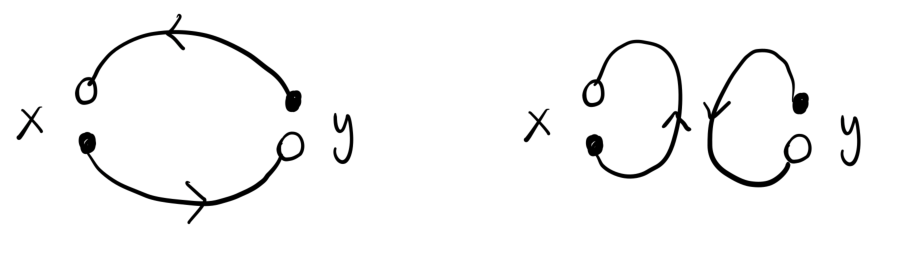
\includegraphics[width=\textwidth]{figs/connected_disconnected.pdf}
\caption{Examples of connected (left) and disconnected (right) diagrams
between spacetime points $x$ and $y$. The arrows indicate the direction of
propagation. Any vertical pair of open and closed circles can be interpreted as
a meson.}
\label{fig:contraction}
\end{figure}

The above computation is an example of a fermion {\it contraction}\index{contraction}.
Equation \eqref{eq:contraction} can be interpreted as follows: The propagator
$D^{-1}_u$ propagates a $u$ quark from $y$ to $x$; simultaneously, the
$D^{-1}_d$ propagates a $d$ quark from $x$ to $y$. The corresponding Feynman
diagram is referred to as a {\it connected}\index{connected diagram} 
diagram. This is shown
schematically in \figref{fig:contraction} (left).\footnote{By doing a hopping
parameter expansion, one can show that $D^{-1}$ can be expressed as a weighted
sum over all possible, non-backtracking paths from $y$ to $x$. So the directed lines 
shown in the \figref{fig:contraction} can be thought of as shorthand
for such sums.}

Using the same kinds of manipulations as in the contraction
\eqref{eq:contraction}, one can show that correlators of 
isosinglet operators of the form
$X=\left(\bar{u}\Gamma u+\bar{d}\Gamma d\right)/\sqrt{2}$ become
\begin{equation}\begin{aligned}\label{eq:disconnectedContribution}
2\ev{X(x)\bar{X}(y)}_F&=
-\tr\left[\Gamma D_u^{-1}(x,y)\Gamma D_u^{-1}(y,x)\right]\\
&~~~~+\tr\left[\Gamma D_u^{-1}(x,x)\right]\tr\left[\Gamma D_u^{-1}(y,y)\right]\\
&~~~~+\tr\left[\Gamma D_u^{-1}(x,x)\right]\tr\left[\Gamma D_d^{-1}(y,y)\right]
+(u\leftrightarrow d).
\end{aligned}\end{equation}
Here we see the appearance of {\it disconnected}\index{disconnected diagram}
diagrams, like $\tr\Gamma D^{_1}(x,x)$, which can be visualized as in
\figref{fig:contraction} (right). These diagrams propagate a quark from a point
$x$ back to $x$. Correlators of the form
$X=\left(\bar{u}\Gamma u-\bar{d}\Gamma d\right)/\sqrt{2}$, like the $I_z=0$
component of the isotriplet, are exactly the same as
\equatref{eq:disconnectedContribution}, except that there appears a relative
minus sign between $u$ and $d$ terms. Computations that set $m_u=m_d$, i.e.
{\it isospin symmetric}\index{isospin!symmetric calculation} calculations, have
the benefit that the disconnected pieces cancel out. This turns out to be
especially convenient, as disconnected diagrams are more expensive to
compute than connected ones.

We note that states of definite spatial momentum $\vec{p}$ can be obtained by
Fourier transforming out the spatial sites, similar to \equatref{eq:fourierLat}.
In this way, the time component $t$ is left free, and the resulting
transform $\tilde{X}\left(\vec{p},t\right)$, being a sum over all sites on the
time-slice $t$, is interpreted as living on the time-slice. 

We close by giving a final formula to compute hadron correlators on the lattice,
exemplifying the case of a connected meson interpolator. Combining
Eqs.~\eqref{eq:evfact}, \eqref{eq:evferm}, \eqref{eq:contraction}, and
the Matthews-Salam formula, we arrive at
\begin{equation}\label{eq:mesonCorrFormula}
\ev{X(x)\bar{X}(y)}=-\frac{1}{Z}
\int\DD U e^{-S_G}\det D_u\det D_d \tr\left[\Gamma D_u^{-1}(x,y)\Gamma
D_d^{-1}(y,x)\right].
\end{equation}

\section{Pseudofermions}\label{sec:pseudofermions}

As discussed in \secref{sec:grassmann}, the Matthews-Salam formula
lets us integrate out the fermion fields, and we are left with
the determinant of a very large matrix, the Dirac matrix, in
our integration measure. Computing this determinant directly
is not computationally feasible. Let's follow a nice presentation
from Ref.~\cite{degrand_lattice_2006} to learn how to approach
simulating dynamical fermions in spite of this difficulty.

The partition function for a single fermion species is
\begin{equation}\begin{aligned}
  Z&=\int\DD U\DD\bar\psi\DD\psi e^{-S_G-\bar\psi D\psi}
   &=\int\DD U \det D\,e^{-S_G}.
\end{aligned}\end{equation}
As we can see in \eqref{eq:diracPositionBasis}, we think of $D$ as a matrix in
the basis of space-time sites, i.e. there is an element for each pair of
space-time points. Even though it is a sparse matrix, its dimensionality is
still impossibly huge, and hence computing determinants in a straightforward
manner is computationally not feasible\footnote{As discussed with
staggered fermions, we will want to take
square roots and fourth roots of the Dirac operator. These rooted matrices
have even more nonzero entries, exacerbating the problem significantly.
It should be that the further one gets from the diagonal, the smaller
the entries become, and in the continuum limit, $D$ 
should become local\index{local}. It should be noted that
the time complexity of
computing the determinant of an $N\times N$ matrix
is usually $\order{N^3}$. This is of course algorithm-dependent,
but the lowest I am aware of is still
slower than $\order{N^2}$, which for us would correspond to
the lattice volume squared.}. 

Instead of evaluating the determinant, we approximate it
by introducing 
{\it pseudofermions}~\cite{fucito_proposal_1981,weingarten_physics_1981}.
A pseudofermion $\Phi\equiv\Phi_R+i\Phi_I$ is a color-triplet, complex, 
scalar field. We leverage the formal identity
\begin{equation}\label{eq:pseudofermionIdentity}
\det M \sim \int\DD{\Phi_R}\DD{\Phi_I}\exp\left(-\Phi^\dagger M^{-1}\Phi\right),
\end{equation}
where the squiggle indicates there may be some irrelevant factors 
missing\footnote{Remember that the only important thing when it comes to
predicting observables is that expectation values remain unchanged.
Constant factors always drop out in the ratio. In Gattringer and Lang I
see some factors $\pi^N$, which I do not always see in the literature.}.
Now, it is always crucial that our exponentials can be interpreted
as probabilities; therefore an important question to ask is whether
that exponential is real and bounded.

One way to explore the argument of the above exponential is to decompose
the scalar fields $\Phi$ in terms of eigenvectors of $M$. Assuming $M$
is an $N\times N$ matrix with only nonzero eigenvalues $\lambda_i$, 
we can write
\begin{equation}
\Phi^\dagger M^{-1}\Phi=\sum_{i=1}^N
\left(\Phi^\dagger\psi\right)_i\frac{1}{\lambda_i}\left(\psi^\dagger\Phi\right)_i.
\end{equation}
The projections of $\Phi$ onto the eigenstates of $M$ are complex
conjugates, so if the eigenvalues were positive, we would be guaranteed that
$\Phi^\dagger M^{-1}\Phi$ is positive. The trick then is to look
out for an operator $M$ with positive eigenvalues.

In \secref{sec:signProblem} we will see that most Dirac operators $D$ used in
lattice field theory are $\gamma_5$-hermitian\index{hermitian},
which means they obey
\begin{equation}
D^\dagger=\gamma_5 D \gamma_5.
\end{equation}
In that Section, we will show this guarantees
\begin{equation}
\det D = \det D^\dagger,
\end{equation}
and hence if we choose $M=D^\dagger D$, we will have
by \equatref{eq:pseudofermionIdentity}
\begin{equation}\label{eq:twoPseudofermionFlavors}
\left(\det D\right)^2 
=\det D^\dagger D 
\sim \int\DD{\Phi_R}\DD{\Phi_I}
\exp\left(-\Phi^\dagger \left(D^\dagger D\right)^{-1}\Phi\right),
\end{equation}
i.e. we will be able to rewrite the fermion determinants corresponding
to a system with two identical flavors of quark in a way that guarantees
we can use a Markov chain.

An important practical point to consider is how to generate $\Phi$ according to
the distribution \equatref{eq:twoPseudofermionFlavors}. Let $R$ be a random
vector such that
\begin{equation}
\Phi=D^\dagger R.
\end{equation}
Then if we draw $R$ from a Gaussian, i.e. if we draw
according to $\exp\left(-R^\dagger R\right)$, we are guaranteed that
$\Phi$ will be distributed as desired.
\bibliographystyle{unsrtnat}
\bibliography{bibliography}

\chapter{LFT: Computer Implementation}\label{ch:MCMC}

As discussed in \secref{sec:haar}, expectation values of 
physical observables $X$ in pure $\SU(N_c)$ LGT
are given by functional integrals
\begin{equation}\label{eq:exobs}
  \ev{X}=\frac{1}{Z}\int\DD{U}e^{-S(U)}X(U).
\end{equation}
Even though the integral~\eqref{eq:exobs} is well defined on a lattice
because there are 
finitely many sites, it is not feasible to evaluate it numerically; even
relatively small lattices have $4\times10^4$ links. The goal of our
simulation is to estimate $\ev{X}$ by randomly generating configurations,
distributed with probability $e^{-S}$,
and on each configuration, making a measurement $X_i$. The average 
\begin{equation}\label{eq:arithmeticaverage}
  \bar{X}=\frac{1}{\nconf}\sum_{i=1}^{\nconf} X_i
\end{equation}
serves as the estimator.

The strategy of carrying out a statistical computation using random sampling
goes under the name of {\it Monte Carlo}\index{Monte Carlo} 
algorithms\footnote{The idea of Monte Carlo algorithms dates back to the 1940s.
Stanislav Ulam wanted to know the probability of winning a game of Solitaire.
The calculation turned out to be too complicated to do by hand, so he wanted to
estimate this by playing repeated games, then calculating
$$
{\rm win\ chance}\approx\frac{\rm number\ of\ wins}{\rm number\ of\ games}.
$$
Of course this is tremendously tedious; it is much more appropriate for a
computer. Other scientists working with him at Los Alamos such as John von
Neumann and Nicholas Metropolis are early pioneers of this method.}.
The strategy of drawing these random configurations is to use a
Markov chain, and hence the backbone of a lattice calculation is
often referred to as {\it Markov chain Monte Carlo} (MCMC).
Further details on MCMC methods can be found in, for instance, 
Ref.~\cite{berg_markov_2004,gattringer_quantum_2010}. 


\section{Markov chain Monte Carlo}\label{sec:MCMCintro}

To generate our configurations, we start from some arbitrary configuration
$C_0$ and construct a stochastic sequence of configurations. 
Configuration $C_i$ is generated based on\index{update}
configuration $C_{i-1}$, which we call an {\it update} or {\it Markov
step}
The result is a {\it Markov chain}
\begin{equation}
  C_0\to C_1\to C_2\to...
\end{equation}
of configurations. 

\index{MCMC}
{\it Markov chain Monte Carlo} (MCMC) is characterized by the probability 
$W^{CC'}\equiv\pr{C'|C}$, the probability to jump to configuration 
$C'$ given that the system started in configuration $C$.
The MCMC {\it transition matrix}\index{transition matrix}
\begin{equation}
  W\equiv\Big(W^{CC'}\Big)
\end{equation}
is constructed to bring the system to {\it equilibrium}.
In equilibrium, the chain should have no sinks or sources of probability,
which means that the probability of jumping into a configuration $C'$
should be the same as jumping out of $C'$. This property
is called {\it balance}\index{balance}
\begin{equation}\label{eq:balance}
    \sum\limits_CW^{CC'}\pr{C}=
    \sum\limits_CW^{C'C}\pr{C'},
\end{equation}
with the LHS representing the total probability to end up in $C'$ and
the RHS representing the probability to transition out of $C'$.
If $W$ satisfies
\begin{enumerate}
  \item {\it ergodicity},\index{ergodic} i.e.
        \begin{equation}\label{eq:ergodicity}
          \pr{C}>0\;\;\text{and}\;\;\pr{C'}>0\;\;\Rightarrow\;\;
          \exists\;n\in\N\;\;\text{s.t.}\;\;\big(W^n\big)^{CC'}>0,
        \end{equation}
        which means that every possible configuration is accessible from
        any other configuration in a finite number\footnote{In practice,
        it's important that $n$ is not too large, otherwise some configurations
        will be sampled poorly. In a sense, this is the problem with
        topological freezing\index{topological!freezing}
        in \secref{sec:toplat}.} of Markov steps;
  \item {\it normalization},\index{normalization} i.e.
        \begin{equation}
          \sum\limits_{C'}W^{CC'}=1,
        \end{equation}
        which means that starting from configuration $C$ you have
        to move somewhere;
  \item and balance, 
\end{enumerate}
then the Markov process is guaranteed to bring the ensemble toward 
equilibrium. Using normalization, one finds from \equatref{eq:balance}
\begin{equation}\label{eq:eigenProb}
    \sum\limits_CW^{CC'}\pr{C}=\pr{C'},
\end{equation}
which shows that the equilibrium distribution is a fixed point of
the Markov chain\footnote{Above, we called $W^{CC'}$ a transition matrix.
Equation~\eqref{eq:eigenProb} shows that we can think of the equilibrium
distribution as an eigenvector of $W$ with eigenvalue 1. Each component
of this vector thus yields the probability of a particular configuration.}. 

\index{Metropolis step}
Here and the following two sections,
we omit the Lorentz index and space-time point from link variables to
avoid clutter.  We use $U$ to indicate the to-be-updated link, 
$U^\sqcup$ to indicate the staple matrix attached to $U$, and
$U'$ to indicate a trial link. We will use the Boltzmann
distribution $\pr{C}\propto e^{-S_C}$.

One trivial way to satisfy the balance condition~\eqref{eq:balance} is
to find an update that satisfies it term-by-term. For such an update, 
\begin{equation}\label{eq:detailedbalance}\index{detailed balance}
    W^{CC'}\pr{C}=W^{C'C}\pr{C'}.
\end{equation}
This property is known as {\it detailed balance}.
One of the most well-known Monte Carlo updates that satisfies detailed
balance is the {\it Metropolis algorithm}~\cite{metropolis_equation_1953}. 
In the Metropolis algorithm, a trial configuration $C'$ is selected 
with some probability distribution $\prt{C'|C}$. Then $C'$
is accepted with likelihood
\begin{equation}\label{eq:metupdate}
  \pr{C\to C'}=\min\left[1,\frac{\prt{C|C'}e^{-S_{C'}}}
    {\prt{C'|C}e^{-S_C}}\right],
\end{equation}
where $S_C$ is the action corresponding to $C$. 
If $C'$ is rejected, the unchanged configuration is counted
in the Markov chain. The total probability
to transition from $C$ to $C'$ using this strategy is 
\begin{equation}\label{eq:MCMCtransition}
W^{CC'}=\prt{C'|C}\pr{C\to C'}, 
\end{equation}
and using this fact, one
can show that this update satisfies detailed balance.

The Metropolis algorithm is in some sense the most standard Markov chain
algorithm used in lattice calculations, with the acceptance step
\equatref{eq:metupdate} being the most crucial part, in the sense that
it guarantees your configuration is drawn with the correct probability.
A Markov algorithm that concludes with the acceptance step is
said to be an\index{exact algorithm} {\it exact algorithm}\footnote{One
could imagine update steps that may not be guaranteed to draw configurations
from the desired distribution. This can be corrected by simply adding
the acceptance step at the end, and the algorithm is still exact.
One may neglect this acceptance step at the end, if one has reason to
believe the configuration is still drawn appropriately, but in such
instances the algorithm is not exact anymore.}.

In general, one could choose a trial configuration uniformly at random
from $\SU(N_c)$. On the other hand, as discussed above, if the trial
configuration increases the action substantially, then by
\equatref{eq:metupdate}, this trial is exponentially unlikely to
be accepted. If we are constantly suggesting such configurations,
we will make little movement in configuration space.
What makes an update efficient then is to suggest configurations that
have reasonable acceptance probabilities to begin with. This
strategy is often called {\it importance sampling}\index{importance sampling}.


\section{General code structure}

Now that we have introduced MCMC, we can sketch the
general code structure of an LFT simulation. 

Typically, simulations use {\it local updates}, which
means we update the links one at a time. This is usually done in a systematic order,
because there is some computational advantage compared to updating in a
random order~\cite{berg_markov_2004}. 
An updating {\it sweep}\index{sweep} updates every link on the lattice once. 

An MCMC simulation of LFT then broadly consists of these essential steps:
\begin{enumerate}
  \item {\it Initialization}: The first thing to do is get everything ready for
        the simulation. This includes initializing the random number generator,
        and setting up an initial configuration.
  \item {\it Equilibration} or {\it thermalization}:
        \index{equilibration}\index{thermalization}
        To avoid over-sampling rare configurations,
        one must perform many sweeps to bring the system to its equilibrium 
        distribution. The structure of this section looks like 
        \begin{verbatim}
        do from n=1 to n=nequi 
          call MCMC update
        end do
        \end{verbatim}
  \item {\it Configuration generation}: One we are in the equilibrium
        distribution, we want to generate configurations on which we can
        perform measurements. To help reduce correlations between
        measurements, multiple updating sweeps are performed in between.
        This section is structured as
        \begin{verbatim}
        do from n=1 to n=nconf
          do from n=1 to n=ndiscarded
            call MCMC update
          end do
          save configuration 
        end do
        \end{verbatim}
  \item {\it Measurements}: Now that we have a good sample of configuration
        space, we are ready to perform measurements there. Some measurements
        can be take {\it in situ}, i.e. they are incredibly cheap and can be
        calculated the moment the configuration is saved. Measurements of this
        type include simple link products like the Polyakov loop. More expensive
        observables may require inverting a Dirac matrix thousands of times, 
        gauge fixing, or smoothing. For such observables it is better to
        have separate code that runs on the saved configurations. This
        code is structured as
        \begin{verbatim}
        do from n=1 to n=nconf
          take measurement 
        end do
        \end{verbatim}
\end{enumerate}

The details of the above steps, especially the MCMC update, depend on what
physics are being simulated. In the following, we discuss some strategies for
generating new gauge fields from old ones.


\subsection{Update: Heat bath}\index{heat bath}

The {\it heat bath} (HB) algorithm is designed to tackle pure $\SU(N_c)$
systems. Here, we construct our trial probability distribution to draw from the
Boltzmann distribution to begin with. Thus no formal accept/reject
step is required\footnote{The Kennedy-Pendleton algorithm has a sort
of accept/reject step on one of the random variables to ensure that
variable is drawn from the correct distribution.}. For pure gauge
simulations, it is common practice to generate a new configuration 
an old one by updating one link. 
For the $\SU(N_c)$ HB algorithm, the trial link distribution is
\begin{equation}\label{eq:PTdist}
  \dd{\prt{U'}}\propto \dd U'\exp\left(\frac{\beta}{N_c}\,\tr\,
  U'U^\sqcup\right).
\end{equation}
This construction also satisfies detailed balance. 
Numerically, the trick is to map \equatref{eq:PTdist} to a set
of real, random variables, which have to be specially
generated to reproduce the desired distribution.
A common strategy for doing this for the gauge group $\SU(2)$,
often referred to as the {\it Kennedy-Pendleton}\index{heat
bath!Kennedy-Pendleton} algorithm, is explained in an elementary way 
in Ref.~\cite{gattringer_quantum_2010}; the original papers are
Refs.~\cite{fabricius_heat_1984,kennedy_improved_1985}.

When $N_c>2$, this strategy is extended by leveraging the fact
that $\SU(2)\leq\SU(N_c)$; in general, an $\SU(N_c)$ matrix
can be broken down into $N_c(N_c-1)/2$ 
$\SU(2)$ submatrices~\cite{cabibbo_new_1982}. One generates each
$\SU(2)$ submatrix using the above HB, then reconstructs
the $\SU(N_c)$ matrix from those.

%Single link Metropolis or HB updates of links carried out in a systematic 
%(as opposed to random) order fulfill balance, but do not
%fulfill detailed balance.

\subsection{Update: Over-relaxation}\index{over-relaxation}

An additional useful update for $\SU(N_c)$ is the 
{\it over-relaxation}\index{over-relaxation} (OR) update. 
Adler introduced OR algorithms \cite{adler_over-relaxation_1981} and 
they were further developed by Creutz \cite{creutz_overrelaxation_1987} 
and others. The idea of the OR algorithm is to speed up relaxation 
by generating a group element ``far away" from $U$ without
destroying equilibrium, which for $\SU(2)$ is achieved by keeping that action
constant. 
This update is not random in any way, but rather serves to move you around
in configuration space without impacting the acceptance rate too much.

More precisely let $U\in\SU(2)$ and suppose we have some method of
choosing another link variable $U_0$ that maximizes
the action for this staple.  We assume that this method of selection has no
dependence on $U$.  Pick some element $V\in\SU(2)$ such that $U=VU_0$; viewed
in this way, $U$ is ``on one side of $U_0$," and the element 
``on the other side" is $U'=V^{-1}U_0$.  Note that
\begin{equation}
  V=U U_0^{-1},
\end{equation}
which implies
\begin{equation}
  U' = U_0 U^{-1} U_0.
\end{equation}
This manner of constructing a new link variable $U'$, which generates
a group element ``far away" from $U$, is what we mean by over-relaxation.

In principle an OR update should be more efficient than a Monte
Carlo update. This is because we chose the new link variable to be two
group elements away from the old one, thrusting us further
along configuration space. However unlike Metropolis updates, OR updates 
only sample the subspace of constant action, and are therefore not ergodic. 
Hence to ensure an approach to equilibrium, they must be supplemented with, 
for instance, HB updates.

For $\SU(2)$, the update is given by
\begin{equation}\label{eq:ORupdate}
  U\to U'=\frac{1}{\det U^\sqcup}\left(U^\sqcup UU^\sqcup\right)^\dagger.
\end{equation}
\begin{proposition}{}{OR}\label{prp:OR}
  This update does not change the $\SU(2)$ Wilson action.
  \begin{proof}
   Since $\det(kA)=k^n\det A$ for any constant $k$ and $n\times n$ matrix $A$,
   one can show that the sum of two $\SU(2)$ matrices is proportional
   to an $\SU(2)$ matrix. Hence we can write
    $$
      U^\sqcup=u^\sqcup\sqrt{\det U^\sqcup}
    $$
    where $u^\sqcup\in\SU(2)$. After updating, the local contribution
    to the Wilson action becomes
    \begin{equation*}
      \tr U'U^\sqcup =\frac{1}{\det U^\sqcup}\tr
                       \left(U^\sqcup UU^\sqcup\right)^\dagger
                     =\tr U^\sqcup U\left(u^\sqcup\right)^\dagger u^\sqcup
                     =\tr U^\sqcup U,
    \end{equation*}
    which is what it was originally.
  \end{proof}
\end{proposition}

This simple 
behavior is special to $\U(1)$ and $\SU(2)$ LGT. 
For $N_c>2$, one can carry out OR updates on the $\SU(2)$ subspaces of the
$\SU(N_c)$ matrix. This in general does not keep the action constant, but it
does change the action only very little. Hence it is a good choice to supplement
HB updates for $\SU(N_c)$ gauge fields in general. 

\subsection{Update: Over-relaxation gauge fixing}\label{sec:ORgaugefix}
\index{gauge!fixing}

In general expectation values of gauge-dependent quantities are zero.
Nevertheless there are rare occasions where it is useful to calculate
a quantity in a particular gauge, which can then be related to some
other physical quantity. In this section we cover an OR
algorithm that fixes gauge configurations to the {\it Coulomb} or 
{\it Landau} gauges.\index{gauge!Coulomb}\index{gauge!Landau}

In the continuum such gauges are given by the condition
\begin{equation}
  \partial_\mu A_\mu=0,
\end{equation}
where $\mu$ runs over only spatial directions for the Coulomb gauge, and
over all four directions for the Lorentz gauge. On the lattice, these 
{\it gauge conditions}\index{gauge!condition} are discretized as
\begin{equation}
  \Delta(x)\equiv A_\mu(x)-A_\mu(x-a\hat\mu) =0.
\end{equation}

\begin{proposition}{}{ORgf}
A gauge satisfying $\Delta(x)=0$ is achieved by extremizing
$$
  F\equiv-\Re\tr\sum_{x,\mu} g(x) U_\mu(x) g^\dagger(x+a\hat{\mu})
$$
\begin{proof}
Any gauge matrix can be written
$$
  g=e^{is^aT^a},
$$
where $s^a\in\R$ and $T^a$ are the generators of the Lie group. We want
to find the special $g_0$ that extremizes $F$; this is equivalent to finding
the $s_0$ that extremizes it. We will look in the vicinity of such a
gauge, i.e. look at gauges 
$$e^{i\tau^a T^a}, \qquad\tau\equiv s-s_0$$
with $\tau$ small. Then
\begin{equation*}\begin{aligned}
  F&=-\Re\tr\sum_{x,\mu}&&
      e^{i\tau^a(x)T^a}\,e^{iaA^b_\mu(x)T^b}\,e^{-i\tau^c(x+a\hat\mu)T^c}\\
   &\approx &&\big(\id+i\tau^a(x)T^a\big)
        \big(\id+iaA_\mu^b(x)T^b\big)
        \big(\id-i\tau^c(x+a\hat\mu)T^c\big)\\
   &\approx && \big(\id+a\tau^c(x+a\hat\mu)A_\mu^b(x)T^bT^c
                       -a\tau^a(x)A_\mu^b(x)T^aT^b\big),
\end{aligned}\end{equation*} 
where we have neglected $\order{a^2, a\tau, \tau^2}$ terms and use that
the $T^a$ are traceless. At the extremum, derivatives with respect to $\tau$
will vanish. Exchanging our dummy group summation indices and shifting
the first term by one site (which is allowed because of 
periodic BCs) we find
\begin{equation*}\begin{aligned}
  0=\pdv{F}{\tau^d}
     &=-\Re\tr\sum_{x,\mu}&&a\pdv{\tau^d}
        \left[A_\mu^b(x-a\hat\mu)\tau^c(x)-A_\mu^b(x)\tau^c(x)\right]T^bT^c\\
     &= &&a\left[A_\mu^b(x-a\hat\mu)-A_\mu^b(x)\right]T^bT^d.
\end{aligned}\end{equation*}
In order for the above to vanish, the term in brackets has to vanish,
which completes the proof.
\end{proof}
\end{proposition}
The strategy from here is to minimize $F$. As you can clearly see from
its definition, this can be accomplished through the replacement
\begin{equation}\label{eq:gfORupdate}
U\to U'=gU_\mu g^\dagger,
\end{equation}
which is reminiscent of the OR update~\eqref{eq:ORupdate}. Hence we employ
again OR, i.e. we find the $g$ minimizing $F$ and make the
replacement~\eqref{eq:gfORupdate}. In a similar strategy as
\propref{prp:OR}, we look at the local update to $F$,
\begin{equation}
  \Re\tr g(x)\sum_\mu\left[U_\mu(x)g^\dagger(x+a\hat\mu)
                        +U_\mu^\dagger(x-a\hat\mu)g^\dagger(x-a\hat\mu)\right]
  \equiv\Re\tr g(x)K(x).
\end{equation}
As before, $K(x)=\sqrt{\det K(x)}\hat K(x)$, where $\hat K(x)\in\SU(2)$.
To extremize $F$, we search for the $g$ rotating everything under the
trace to $\id$, which is clearly
\begin{equation}
  g(x)=K^\dagger(x)/\sqrt{\det K(x)}.
\end{equation} 

We will never achieve the condition $\Delta(x)=0$ on the computer exactly.
A measure of how close we are to satisfying the gauge condition is
\begin{equation}
  \theta\equiv\frac{1}{N_c N_s^3}\sum_x\tr\Delta(x)\Delta^\dagger(x).
\end{equation}
This combination is constructed so that $\theta\in\R$. 

For more information
about using OR to gauge fix, see Ref.~\cite{mandula_efficient_1990}. 
For information about how to implement this on multiple GPUs, see
e.g. Ref.~\cite{schrock_coulomb_2013}.

\subsection{Update: Molecular dynamics}\label{sec:MD}\index{molecular dynamics}

We now discuss one of the most popular updating strategies on the market,
especially when carrying out simulations with dynamical fermions.
For this updating strategy, we leverage an isomorphism between
lattice field theory and a classical statistical mechanical 
ensemble. We will use this
correspondence to find a clever way of suggesting a gauge
configuration, and then ultimately accept or reject it via
a standard Metropolis step.

To start let's imagine a theory with a scalar field $\phi$ on 
the lattice. Then expectation values are computed like
\begin{equation}
\ev{X}=Z^{-1}\int\DD\phi e^{-S[\phi]}X[\phi],~~~~Z\equiv\int\DD\phi
e^{-S[\phi]}.
\end{equation}
Now let
\begin{equation}
H\equiv\frac{1}{2}\sum_{x\in\LAT}P(x)^2+S[\phi],
\end{equation}
where $P$ is a scalar field we will define in a moment. Since $P$ is some other
field, it follows that
\begin{equation}
\ev{X}=Z^{-1}\int\DD\phi\DD P e^{-H[\phi,P]}X[\phi],
~~~~Z\equiv\int\DD\phi\DD P e^{-H[\phi,P]}.
\end{equation}
Now let these fields evolve in Markov time $\tau$ and define
\begin{equation}
\dv{\phi(x)}{\tau}\equiv P(x).
\end{equation}
Then we have defined a classical system where $P$ is the momentum
conjugate to $\phi$. If we evolve $\phi$ and $P$ in $\tau$ according
to Hamilton's equations of motion, the energy is guaranteed to
be a constant. This procedure would yield 100\% acceptance if we
were able to integrate the equations of motion exactly. In practice
there is round off error, and the Metropolis step serves to protect
the probability distribution.

The above example is for a scalar field, which is a simplification of 
Ref.~\cite{callaway_microcanonical_1982},
which does it for $\U(1)$. This was shortly thereafter extended
to fermions~\cite{polonyi_microcanonical_1983}. 
This integration is completely deterministic, and hence does not
capture quantum fluctuations. To capture such quantum behavior,
one can intuitively imagine disturbing Hamilton's equations
with a random noise term. This is is an example of a
stochastic differential equation\footnote{A stochastic differential
equation is a differential equation where you include one
or more random forces. A simple example is the Langevin equation
$$
m \dv{v}{t}=-\lambda v+\eta(t)
$$
describing the Brownian motion of a particle of mass $m$
and velocity $v$ in a fluid. Here $\lambda$ is the drag, and
$\eta$ is a Gaussian-distributed noise term representing
random collisions of the particle with other particles in the fluid.
At a fixed value of the noise, such equations can be solved.
It becomes challenging when one wants to average over $\eta$.
}
like the Langevin equation, which can be used to model the inherent
randomness of the underlying quantum field 
theory~\cite{parisi_perturbation_1981}.
Inspired by this, we might consider to give the conjugate momentum
random kicks, following the microcanonical path in between.
This strategy is often called a 
{\it hybrid}~\cite{duane_hybrid_1985} strategy.
If not for numerical rounding error, this strategy would be expected
to generate the correct 
distribution~\cite{duane_theory_1986}.
To correct for numerical error, one can again apply the Metropolis
step as before, which is referred to as 
{\it hybrid Monte Carlo}\index{Monte Carlo!hybrid} (HMC).

Applying a series of molecular dynamics steps is usually called
a {\it trajectory}\index{trajectory}, after which comes the
Metropolis step. To fulfill detailed balance\footnote{Remember
we need this in order to ensure that the typical accept/reject
based on the configuration generated by the molecular dynamics
is a valid Metropolis step.}, we need to ensure
that our integration scheme
\begin{enumerate}
  \item preserves the integration measure $\DD\phi\DD P$; and
  \item is reversible.
\end{enumerate}
A commonly used scheme that fulfills these demands is known as the
{\it leapfrog} algorithm. Under this scheme, $\phi$ integrates
in $N$ steps of Monte Carlo length $\epsilon$, while $P$
starts with a step of length $\epsilon/2$, followed by $N-1$
steps of length $\epsilon$, and a final step of length $\epsilon/2$.
You can find an elementary proof that the leapfrog preserves area
and is reversible in Ref.~\cite{gattringer_quantum_2010}.
There one also finds a proof that the Metropolis fulfills detailed balance.

Let us synthesize what we have discussed to introduce an updating scheme that
represents a system of two indentical fermions with gauge interaction
at zero chemical potential.
This scheme for staggered fermions was first made explicit
in Ref.~\cite{gottlieb_hybrid-molecular-dynamics_1987}.
As discussed in \secref{sec:pseudofermions}, the most efficient way
to treat the determinant of the Dirac matrix is using pseudofermions.
Hence our path integral is\index{pseudofermion}
\begin{equation}\begin{aligned}\label{eq:twoFlavorRHMC}
Z&=\int\DD{U}\left(\det D\right)^2e^{-S_G}\\
&=
\int\DD{\Phi_R}\DD{\Phi_I}\DD{U} 
e^{-S_G-\Phi^\dagger\left(D^\dagger D\right)^{-1}\Phi},
\end{aligned}\end{equation}
where we have introduced a three-color, complex scalar field
$\Phi=\Phi_R+i\Phi_I$, the pseudofermion field.
In \secref{sec:pseudofermions} we stressed that the treatment of two identical
fermions was important since it lets us put a $D^\dagger D$ in the
exponential, which makes it a well defined probability distribution.
We also saw that we can draw our pseudofermions according to the
above distribution if we define $\Phi=D^\dagger R$ and draw $R$ from
$\exp\left(-R^\dagger R\right)$. The strategy then goes:
\begin{enumerate}
\item Generate Gaussian $R$.
\item Solve $\Phi=D^\dagger R$ to get $\Phi$.
\item Given your starting configuration $U$ generate conjugate
momenta.
\item Keeping $\Phi$ fixed, use the molecular dynamics strategy
to integrate along a short trajectory, yielding a proposal for $U$.
\item Do a Metropolis accept/reject at the end of the trajectory for $U$.
\end{enumerate}

Let us discuss steps 2-4 in a little more detail; in particular we would like to
understand how the molecular dynamics works for $\SU(3)$. We express our gauge
field as
\begin{equation}
U_\mu=e^{i\omega_\mu^aT^a}=e^{iA_\mu}.
\end{equation}
We will therefore think of our Hamiltonian as a function of the
generalized coordinates $A_\mu$, or equivalently when convenient,
$\omega_\mu^a$. The corresponding conjugate momenta are
\begin{equation}
P_\mu=P^a_\mu T^a.
\end{equation}
The steps taken in the leapfrog change the momentum. With our fictitous 
Hamiltonian in mind, what we seek is a force, i.e. a gradient of
the effective action. Looking at \equatref{eq:twoFlavorRHMC} our effective
action is
\begin{equation}
S_{\rm eff}=-S_G-\Phi^\dagger\left(D^\dagger D\right)^{-1}\Phi,
\end{equation}
and the force is
\begin{equation}
f=T^a\nabla^aS_{\rm eff}.
\end{equation}
The leapfrog thus proceeds in steps $\epsilon f$.

Based on the effective action, the force can be divided into the
{\it gauge force} and {\it fermion force}. The fermion force thus 
depends on the chosen discretization. For example with a straightforward Wilson
gauge action, whose contribution at $U$ has the form
\begin{equation}
-\frac{\beta}{6}\tr\left(UA+A^\dagger U^\dagger\right),
\end{equation}
where $A$ is the staple sum. Using \equatref{eq:lieDeriv},
the fact that the derivative lies in the Lie algebra,
which lets you express it as a linear combination of the generators,
and \eqref{eq:SUNnorm}, the gauge force comes out to be
\begin{equation}
f_G=-\frac{i\beta}{12}\left(UA-A^\dagger U^\dagger\right).
\end{equation}
Meanwhile, using \propref{prp:MATwrtSCLinv}, 
the fermion force can be written 
\begin{equation}
f_{\rm ferm}^a=
-T^a\left(\left(D^\dagger D\right)^{-1}\Phi\right)^\dagger
\left(\pdv{D}{\omega^a}D^\dagger+D\pdv{D^\dagger}{\omega^a}\right)
\left(\left(D^\dagger D\right)^{-1}\Phi\right).
\end{equation}
This shows that the inverse of $D^\dagger D$ must be computed
at each step of the molecular dynamics, which is far and away
the most expensive part.

Both here and in Step 2 we need to compute inverses of extremely
large matrices. One of the most efficient ways to approach this,
and indeed the strategy taken by codes such as 
QUDA, 
Grid, and
$\simulat$, is to use the conjugate gradient.
The difficulty of computing the inverse increases
substantially according to the smallest eigenvalue of $D$,
as mentioned in \secref{sec:numerics}. As a result
one may need to employ an SVD or a
{\it force filter}\index{force!filter}, which artificially
shifts low eigenmodes by an amount $\delta$.

\section{The HISQ force}\label{sec:HISQforce}

The HISQ action, discussed in \secref{sec:stagg} and \secref{sec:HISQ},
is widely used in state-of-the-art lattice calculations. 
Here we discuss the computer implementation of HISQ fermions. 
Constructing its
force is a bit complicated, as it is a synthesis of many constructs in
those sections along with \secref{sec:MD}. In my view,
implementing HISQ fermions is complicated enough to warrant its own section,
maybe even its own chapter.

We begin by writing down the action itself in a way that is helpful
for computer implementation. We write
\begin{equation}
S_f=\Phi^\dagger\left(D^\dagger D\right)^{-N_f/4}\Phi
=\bra{\Phi}\left(D^{\dagger} D\right)^{-N_f/4}\ket{\Phi},
\end{equation}
where $N_f$ is the number of fermions and $\ket\Phi$ is the pseudofermion field.
For this presentation of the HISQ force, we follow
Ref.~\cite{Wong:2007uz}, and hence switch to bra-ket notation.
Remember, we chose this pseudofermion rewrite to be able to compute the
determinant of the Dirac matrix efficiently. We want a
$D^\dagger D$ in the exponential since it has positive eigenvalues,
and hence makes for a well defined probability distribution.

The $D^\dagger D$ would correspond to two identical quarks of that flavor, since
by the Matthews-Salam formula
\begin{equation}
\det D^\dagger D = \det D^\dagger \det D
=\int \dd{\bar{\psi}_f}\dd{\psi_f}\dd{\bar{\psi}_g}\dd{\psi_g}
\exp\left(\bar{\psi}_fD^\dagger\psi_f+\bar{\psi}_gD \psi_g\right).
\end{equation}
The trick to get around this, as done in 
Ref.~\cite{gottlieb_hybrid-molecular-dynamics_1987}, is to define the
$\Phi$ fields on even sites only. This works because $D^\dagger D$ has no
matrix elements connecting even and odd sites. More precisely, if
$D_0$ is the massless part of the Dirac operator, then
\begin{equation}\begin{aligned}
\left(D^\dagger D\right)_{xy}
&=\left(2m\delta_{xz}+D^\dagger_{0,xz}\right)
  \left(2m\delta_{zy}+D_{0,zy}\right)\\
&=4m^2\delta_{xy}+2m\left(D^\dagger_{0,xy}+D_{0,xy}\right)+D^\dagger_{0,xz}D_{0,zy}.
\end{aligned}\end{equation}
The second term in the last line vanishes since $D$ is antihermitian.
The first term is diagonal in the site basis. Similarly $D$ itself always sends
odd to even or vice versa, so $D_0^\dagger D_0$ must preserve parity.
Hence if we write $D^\dagger D$ in a basis organized so even indices come first 
followed by odd, we have a block-diagonal matrix with two copies of
$4m^2+D_0^\dagger D_0$. Restricting to even or odd halves the number of degrees
of freedom, returning us once again to our interpretation of having a single
fermion species.

Finally we have the issue, discussed in
\secref{sec:HISQ}, that staggered fermions lead to four degenerate tastes.
The solution offered in that section is to take the fourth root. In practice,
this fourth root is implemented as a rational 
approximation~\cite{clark_rhmc_2004,clark_rational_2006},
\begin{equation}
\left(D^\dagger D\right)^{-N_f/4}\approx\alpha_0+\sum_l\frac{\alpha_l}{D^\dagger
D+\beta_l}.
\end{equation}
Using the rational approximation to estimate the fourth root in this hybrid
Monte Carlo scheme is called {\it rational hybrid Monte Carlo}\index{RHMC}
(RHMC).


Next we need to open up the $D$. We write\footnote{It is common practice in
lattice publications to use $M$ rather than $D$ to indicate the Dirac matrix.
In that case, $D$ is sometimes used to indicate the (covariant) derivative part.
I took the notation of Gattringer and Lang~\cite{gattringer_quantum_2010}.}
\begin{equation}\begin{aligned}
D(y|x)&=2m\delta_{x,y}
+\sum_\alpha \eta_\alpha(x)\left(\UHISQ_\alpha(x)\delta_{x,y-\hat\alpha}
-\left(\UHISQ_\alpha(x-\hat\alpha)\right)^\dagger\delta_{x,y+\hat\alpha}\right)\\
&\equiv 2m\delta_{x,y}+\dd_{x,y},
\end{aligned}\end{equation}
where $\UHISQ$ is given by \equatref{eq:HISQsmear}:
\begin{equation}
\UHISQ=\mathcal{F}^{\rm Fat7}_{\rm corr}\mathcal{U}\mathcal{F}^{\rm Fat7}U,
\end{equation} 
i.e. we Fat7-smear the thin link, followed
by a reunitarization and then a second-level smear that has some lattice-spacing
corrections built in. The $\eta_\alpha$ are the
staggered phases defined in \equatref{eq:staggeredPhase}.



\section{Improving performance}

The inversion of the Dirac matrix is generally the bottleneck of LFT
simulations. We generally get better throughput as hardware improves, 
but waiting for hardware improvements is not sufficient for completing realistic
simulations in an acceptable amount of time. In \secref{sec:performance} we
already discussed some general methods to get the most out of your hardware.
Here, we will discuss some strategies that are specific to LFT.

\subsection{The Hasenbusch trick}\index{preconditioning!Hasenbusch}

At this point is has been mentioned multiple times that a major bottleneck
of the RHMC algorithm, which as of now is the fastest scheme for
generating configurations with dynamical quarks, is inverting the
Dirac matrix. As discussed in \secref{sec:numerics}, if this matrix
has a poor condition number, it is difficult to invert.
One way to alleviate this problem is to {\it
precondition}\index{preconditioning} the matrix. With this strategy,
we look out for a preconditioner $P$ to transform our to-be-solved equation to
\begin{equation}
DP^{-1}Px=b
\end{equation}
with the hope that $DP^{-1}$ has a better condition number than $D$ had.

Inverting $D$ becomes more costly as the bare quark mass is dialed down.
The {\it Hasenbusch trick}~\cite{hasenbusch_speeding_2001,urbach_hmc_2006}
notes that
\begin{equation}
\det D^{\dagger} D\left(m_l\right)=\det \frac{D^{\dagger}
D\left(m_l\right)}{D^{\dagger} D\left(m_h\right)} \det D^{\dagger}
D\left(m_h\right),
\end{equation}
where $m_l$ indicates some light quark mass and $m_h$ some heavier one.
The heavier masses are then treated with their own pseudofermion integrals.
One can intuitively see how the ratio could plausibly have a lower condition
number than $D^\dagger D(m_l)$: 
if there were a basis that diagonalized both the light and heavy Dirac
operators, the largest eigenvalue of $D^\dagger D(m_l)$ would be attenuated by
the largest eigenvalue of $D^\dagger D(m_h)$, and the same would happen for the
smallest eigenvalues.

\bibliographystyle{unsrtnat}
\bibliography{bibliography}


%We now describe an iterative method to search for the minimum of $\chi^2$.
%Let $a_n$ be the vector of parameters for the $n\nth$ iteration.
%As long as $a$ is in a small enough neighborhood of $a_n$, we can safely
%approximate
%\begin{equation}\label{eq:NRapprox}
%  \chi^2(a)\approx\chi^2(a_n)+(a-a_n)\cdot b
%           +\frac{1}{2}(a-a_n)\,A\,(a-a_n),
%\end{equation}
%where the coefficients of the vector $b$ and the $M\times M$ matrix $A$ 
%are given by the first and second derivatives of $\chi^2$ evaluated at $a_n$.
%In the {\it Newton-Raphson method}\index{Newton-Raphson}, the next 
%iteration $a_{n+1}$ is
%determined from the condition $\nabla\chi^2(a)|_{a=a_{n+1}}=0$,
%which yields
%\begin{equation}\label{eq:NR}
%  a_{n+1}=a_n-A^{-1}b.
%\end{equation}
%If the approximation~\eqref{eq:NRapprox} is not good, one can instead move
%a small step in the direction of the gradient by
%\begin{equation}\label{eq:SD}
%  a_{n+1}=a_n-c\,b,
%\end{equation}
%where $c$ is a constant that is small enough not to overshoot direction
%of steepest descent. This is an example of a {\it steepest descent method}.
%The Levenberg-Marquardt\index{Levenberg-Marquardt} 
%method~\cite{levenberg_method_1944,marquardt_algorithm_1963} 
%varies smoothly between~\equatref{eq:NR} and 
%\eqref{eq:SD}. Steepest descent is used far from the minimum, and 
%then it switches to the Newton-Raphson method when the minimum is approached.

\chapter{LFT: Real Physics on the Lattice}\label{ch:realPhys}

We are now in a position to start tackling some real-world physics using the
methods of LFT. Nowadays lattice calculations inform many branches of particle
physics where ab initio, non-perturbative investigations are useful, for example
when computing CKM matrix elements, when exploring the QCD phase diagram at
low-to-moderate temperature near zero quark chemical potential, hadron
spectroscopy, or learning about the muon anomalous magnetic moment, just to name
a few applications.

It is common in these calculations to set $m_u=m_d\equiv m_l$.
This leads to a small systematic error, because of course the up-
and down-quark masses are not exactly equal in the real world. For most
LQCD calculations this systematic error can be neglected, but for the
highest precision measurements, for instance when calculating
the muon anomalous magnetic moment, they can comprise a substantial fraction of
the overall uncertainty. When it is relevant, this uncertainty
is referred to as\index{strong isospin breaking} {\it strong isospin breaking}.

\section{QCD thermodynamics}\label{sec:QCDtherm} 

This section focuses on the phenomenology I worked on as a postdoc in
Bielefeld, i.e. the phase diagram of QCD. There are many useful reviews
on the market, for instance Ref.~\cite{ding_thermodynamics_2015}.

In the following we will focus on $N_f=2+1$ QCD using HISQ fermions. We are
interested in nonzero $\mu$, which is not accessible directly by the lattice.
One possible strategy is to expand in small $\muh\equiv\mu/T$. For the
pressure, we find\footnote{Note that this combination on the LHS of 
\equatref{eq:pxpac} is unitless. This is because area has units
MeV$^{-2}$ and force has units MeV$^2$.}
\begin{equation}\label{eq:pxpac}
\frac{P}{T^4}=\sum_{ijk}\frac{1}{i!j!k!}\,\chi_{ijk}^{(u)(d)(s)}(T)\,
               \muh_u^i\,\muh_d^j\,\muh_s^k,
\end{equation}
where we have defined the {\it generalized
susceptibility}\index{generalized susceptibility}
\begin{equation}
\chi_{ijk}^{(u)(d)(s)}(T)
  \equiv\frac{\partial^{\,i+j+k}\,P/T^4}{\partial\muh_u^i\partial\muh_d^j
                                       \partial\muh_s^k}\Big|_{\muh=0}.
\end{equation}
Some example generalized susceptibilities could be
\begin{equation}
  \chi_2^u=\frac{\partial^2}{\partial\muh_u^2}\frac{P}{T^4}
  ~~~~\text{or}~~~~
  \chi_{11}^{us}=\frac{\partial^2}{\partial\muh_u\partial\muh_s}\frac{P}{T^4}.
\end{equation}

Another set of useful relations is between chemical potentials in the flavor
$(u,d,s)$ basis and the conserved charge $(B,Q,S)$ basis\footnote{Yet a further
possible basis of conserved charges is the $(B,I,S)$ basis with isospin $I\equiv I_3$.
For the purpose of distinguishing between $u$ and $d$ quarks only, one can use
either $I$ or $Q$.
To learn more in detail about isospin, see \secref{sec:isohyper}.}, i.e. the basis
of baryon number, electric charge, and strangeness. These relations 
are\footnote{A mnemonic to remember these relations is to ask what each quark
contributes to a system. For example a strange quark makes 1/3 of a baryon,
adds charge -1/3, and subtracts 1 from the strangeness.}
\begin{equation}\begin{aligned}\label{eq:quark-conservedCharge}
  \mu_u &= \frac{1}{3}\mu_B + \frac{2}{3}\mu_Q\\
  \mu_d &= \frac{1}{3}\mu_B - \frac{1}{3}\mu_Q\\
  \mu_s &= \frac{1}{3}\mu_B - \frac{1}{3}\mu_Q - \mu_S.
\end{aligned}\end{equation}
These relations are needed whenever one is interested in {\it conserved
charge fluctuations},\index{conserved charge fluctuation} i.e. susceptibilities like
\begin{equation}
\chi_{ijk}^{(B)(Q)(S)}(T)
  \equiv\frac{\partial^{\,i+j+k}\,P/T^4}{\partial\muh_B^i\partial\muh_Q^j
                                       \partial\muh_S^k}\Big|_{\muh=0}.
\end{equation}
Since none of the conserved charges appears directly in the action, one
instead must decompose a conserved charge derivative into quark derivatives
using \equatref{eq:quark-conservedCharge}. For example 
one finds
\begin{equation}
  \pdv{\mu_B}
   =\sum_f\pdv{\mu_f}{\mu_B}\pdv{\mu_f}
   =\frac{1}{3}\sum_f\pdv{\mu_f}.
\end{equation}

Once we've picked a discretization, we know the action. From the perspective of
practical calculations coming from lattices, it is hence desirable to express
these formulas in terms of the partition function $Z$. From~\equatref{eq:pgrand}
we have
\begin{equation}
  \frac{P}{T^4}=\frac{1}{VT^3}\log Z,
\end{equation}
where as usual $V=(aN_s)^3$ and $T=1/aN_\tau$.
Hence we can instead
express generalized susceptibilities as
\begin{equation}
\chi_{ijk}^{(u)(d)(s)}(T)
  =\frac{1}{VT^3}\frac{\partial^{\,i+j+k}}{\partial\muh_u^i\partial\muh_d^j
                                       \partial\muh_s^k}\log Z\,\Big|_{\muh=0}.
\end{equation}

When there are $N_f$ flavors and when we use the HISQ action we have,
according to \equatref{eq:HISQdist},
\begin{equation}
  Z=\int\DD U\prod_f (\det D_f)^{1/4}\,e^{-S_G}
\end{equation}
and compute expectation values of the observable $X$ as
\begin{equation}\label{eq:HISQev}
  \ev{X}=\frac{1}{Z}\int\DD U\prod_f(\det D_f)^{1/4}\,e^{-S_G}X.
\end{equation}

Recall that in the grand canonical ensemble, a particle number
$N$ enters\footnote{See \equatref{eq:fugacity}.} 
the Boltzmann factor as $\mu N/T$; so a particle number density 
for a quark flavor $f$ is extracted as\footnote{This is consistent
with \equatref{eq:1stlawgrand}; the factor $T$ switching from
$\mu$ to $\muh$ is compensated in the definition of $\Phi$.}
\begin{equation}\label{eq:nfdensity}
  \frac{1}{V}\,\partial_{\muh_f}\log Z
  =\frac{1}{VZ}\,\partial_{\muh} Z
  =\ev{n_f}.
\end{equation}
In the staggered formulation, all the dependence on $\muh_f$ will be
hidden in $D_f$, so for $f\neq g$ we get
\begin{equation}
  \partial_{\muh_f}D_g = 0.
\end{equation}
Finally we note that, for the purpose of doing Taylor series expansions, it is
useful to remember that the QCD partition function should be blind to charge
conjugation at $\mu_B=0$. This tells us that we should expect only even powers
of $\mu_B$ when using that as the expansion parameter. 

\subsection{Derivative formulas}

We will now derive some formulas which are useful for calculations in QCD
thermodynamics. You can find even more useful formulas for a system of 
$N_f$ identical
fermion flavors in the appendix of Ref.~\cite{allton_thermodynamics_2005}.
For these calculations we will often use\index{ETL formula}
\thmref{thm:exptrlog}, which I refer to here as the ETL formula.

Let $M$ depend on $\alpha\in\C$ and let $y\in\R$. Then from the ETL formula
\begin{equation}\begin{aligned}
  \partial_\alpha(\det M)^y &= y(\det M)^{y-1}\partial_\alpha\det M\\
      &= y(\det M)^{y-1}\exp\left[\tr\log M\right]\partial_\alpha\tr\log M\\
      &= y(\det M)^y \tr M^{-1}\partial_\alpha M.
\end{aligned}\end{equation}
This formula is useful in evaluating derivatives of roots of the fermion
matrix determinant. A final formula useful for matrix derivatives is
\begin{equation}
  \partial_\alpha M^{-1} = - M^{-1}\left(\partial_\alpha M\right) M^{-1}.
\end{equation}

Our goal is to eventually take derivatives of expectation values, so from
\equatref{eq:HISQev} we will need $\muh$-derivatives of the partition 
function. For the following few formulas 
I will assume arbitrarily many non-degenerate
fermion flavors\footnote{I find this helpful to get prefactors that appear
in terms in, e.g., $\chi_2^u$ correct.}. Assuming $S_G$ has no 
$\muh$-dependence, we find
\begin{equation}
  \partial_{\muh}Z = \frac{1}{4}\sum_f 
                      Z\ev{\tr D_f^{-1}\partial_{\muh}D_f}.
\end{equation}
Hence 
\begin{equation}\label{eq:dZinv}
  \partial_{\muh}Z^{-1} = -Z^{-2}\partial_{\muh}Z
                        =\frac{1}{4}\sum_fZ\ev{\tr D_f^{-1}\partial_{\muh}D_f}
\end{equation}
and
\begin{equation}\label{eq:dlogZ}
  \partial_{\muh}\log Z=\frac{1}{4}\sum_f\ev{\tr D_f^{-1}\partial_{\muh}D_f}.
\end{equation}
Comparing \equatref{eq:dlogZ} with \equatref{eq:nfdensity} we find in
the staggered formulation
\begin{equation}
  n_f=\frac{1}{4V}\tr D_f^{-1}\partial_{\muh_f}D_f.
\end{equation} 
Finally using \equatref{eq:dZinv} one quickly derives the following useful formula
for an observable $O$ calculated on HISQ configurations:
\begin{proposition}{}{dO}
\begin{equation*} \partial_{\muh}\ev{O}
       =   \ev{\partial_{\muh}O}
        -\frac{1}{4}\sum_f\ev{\tr D_f^{-1}\partial_{\muh}D_f}\ev{O}
         +\frac{1}{4}\sum_f\ev{O\tr D_f^{-1}\partial_{\muh}D_f}
\end{equation*}
\end{proposition} 
Note that if $\muh=\muh_f$ with $N_f$ degenerate flavors, 
\propref{prp:dO} reduces to eq.~(A3)
in Ref.~\cite{allton_thermodynamics_2005}. Using this Proposition along
with \equatref{eq:dlogZ}, one 
can start expressing generalized susceptibilities in terms of the fermion
matrix. For example one finds for any flavor $f$
\begin{equation}\begin{aligned}
  VT^3\,\chi_2^f =\partial_{\muh_f}^{\,2}\log Z
                 =\, & \frac{1}{16}\ev{\left(\tr D_f^{-1}D_f'\right)^2}
                    -\frac{1}{16}\ev{\tr D_f^{-1}D_f'}^2\\
                   & -\frac{1}{4}\ev{\tr \left(D_f^{-1} D_f'\right)^2}
                    +\frac{1}{4}\ev{\tr D_f^{-1}D_f''},
\end{aligned}\end{equation}
where a prime on $D_f$ indicates a derivative w.r.t. the corresponding chemical
potential $\muh_f$. Similarly for two flavors $f\neq g$ 
\begin{equation}\begin{aligned}
  VT^3\,\chi_{11}^{fg} =\partial_{\muh_f}\partial_{\muh_g}\log Z
                 = \,& \frac{1}{16}\ev{\tr D_f^{-1}D_f'\tr D_g^{-1}D_g'} \\
                   & -\frac{1}{16}\ev{\tr D_f^{-1}D_f'}\ev{\tr D_g^{-1}D_g'}.
\end{aligned}\end{equation}
Using an $N_f=2+1$ HISQ action with $m_l\equiv m_u=m_d$ along with 
\equatref{eq:quark-conservedCharge}, one can figure out how to 
express\footnote{Note that when carrying out calculations like these, to avoid making mistakes,
one should always work with non-degenerate flavors, then allow the flavors to be
degenerate at the end. This way one correctly distinguishes between e.g.
$\chi_{11}^{ll}$ and $\chi_2^l$.} conserved charge fluctuations in terms of 
generalized susceptibilities, such as
\begin{equation}
  \chi_2^B=\frac{1}{9}\left(2\chi_2^l+\chi_2^s+2\chi_{11}^{ll}+4\chi_{11}^{ls}\right)
\end{equation}
and
\begin{equation}
  \chi_2^Q=\frac{1}{9}\left(5\chi_2^l+\chi_2^s-4\chi_{11}^{ll}-2\chi_{11}^{ls}\right).
\end{equation}


\subsection{QCD material parameters}


The speed of sound at fixed control parameter $X$ is defined as
\begin{equation}
  c_X^2=\left(\pdv{p}{\epsilon}\right)_X.
\end{equation}
In a simple (1+1)-$d$ isotropic model of a heavy ion collision, 
sometimes referred to as \index{Bjorken flow}{\it Bjorken flow}, 
assuming a constant $c_s^2$, one can show~\cite{bjorken_highly_1983} 
that the energy density will decrease with proper time $\tau$ as
\begin{equation}
  \epsilon(\tau)=\epsilon(\tau_0)\left(\frac{\tau_0}{\tau}\right)^{1+c_s^2}.
\end{equation}
In this picture one thus finds the system cools with longitudinal expansion
of the fireball according to the speed of sound. % Henrik's thesis is nice
Also in the context of heavy ion collisions, it can be used to look out
for a long-lived fireball, which may coincide with a {\it softest point}
\index{softest point} where the pressure-to-energy-density ratio,
and hence $c_s^2$, attains a minimum\footnote{Another way of looking at
this is that near the crossover as we increase temperature, this
energy serves to change hadronic degrees of freedom to screened
quarks and gluons, rather than changing the pressure.}~\cite{hung_hydrodynamics_1995}.
In the context of neutron stars, $c_s^2$ is interesting since the relationship
between the star masses and radii is influenced by how $c_s^2$ changes with
$n_B$~\cite{ozel_masses_2016}.

The speed of sound has been calculated at $\mu_B=0$ on the 
lattice~\cite{borsanyi_qcd_2010,bazavov_equation_2014,borsanyi_full_2014}.
It has also been calculated using PNJL and NJL 
\index{NJL model}\index{PNJL model}
models\footnote{The Nambu-Jona-Lasinio (NJL)
model~\cite{nambu_dynamical_1961,nambu_dynamical_1961-1} is a low-energy,
effective model of interacting chiral fermions, i.e. it has a 4-fermion
interaction term. This means it's non-renormalizable, so it is not expected
to be a correct description at very high energies.
In the Polyakov-loop-extended NJL (PNJL) model~\cite{meisinger_chiral_1996}, 
one includes the zeroth component of the gauge field. The field is assumed to
be spatially uniform.}~\cite{ghosh_susceptibilities_2006,marty_transport_2013,deb_estimating_2016,motta_isentropic_2020,zhao_thermodynamic_2020};
in the quark-meson coupling
model~\cite{schaefer_thermodynamics_2010,abhishek_transport_2018};
the field correlator
method~\cite{khaidukov_speed_2018,khaidukov_thermodynamics_2019};
and in the quasiparticle method~\cite{mykhaylova_impact_2021}.

\section{The QCD phase diagram}

\begin{figure}
\centering
\vspace{-1cm}
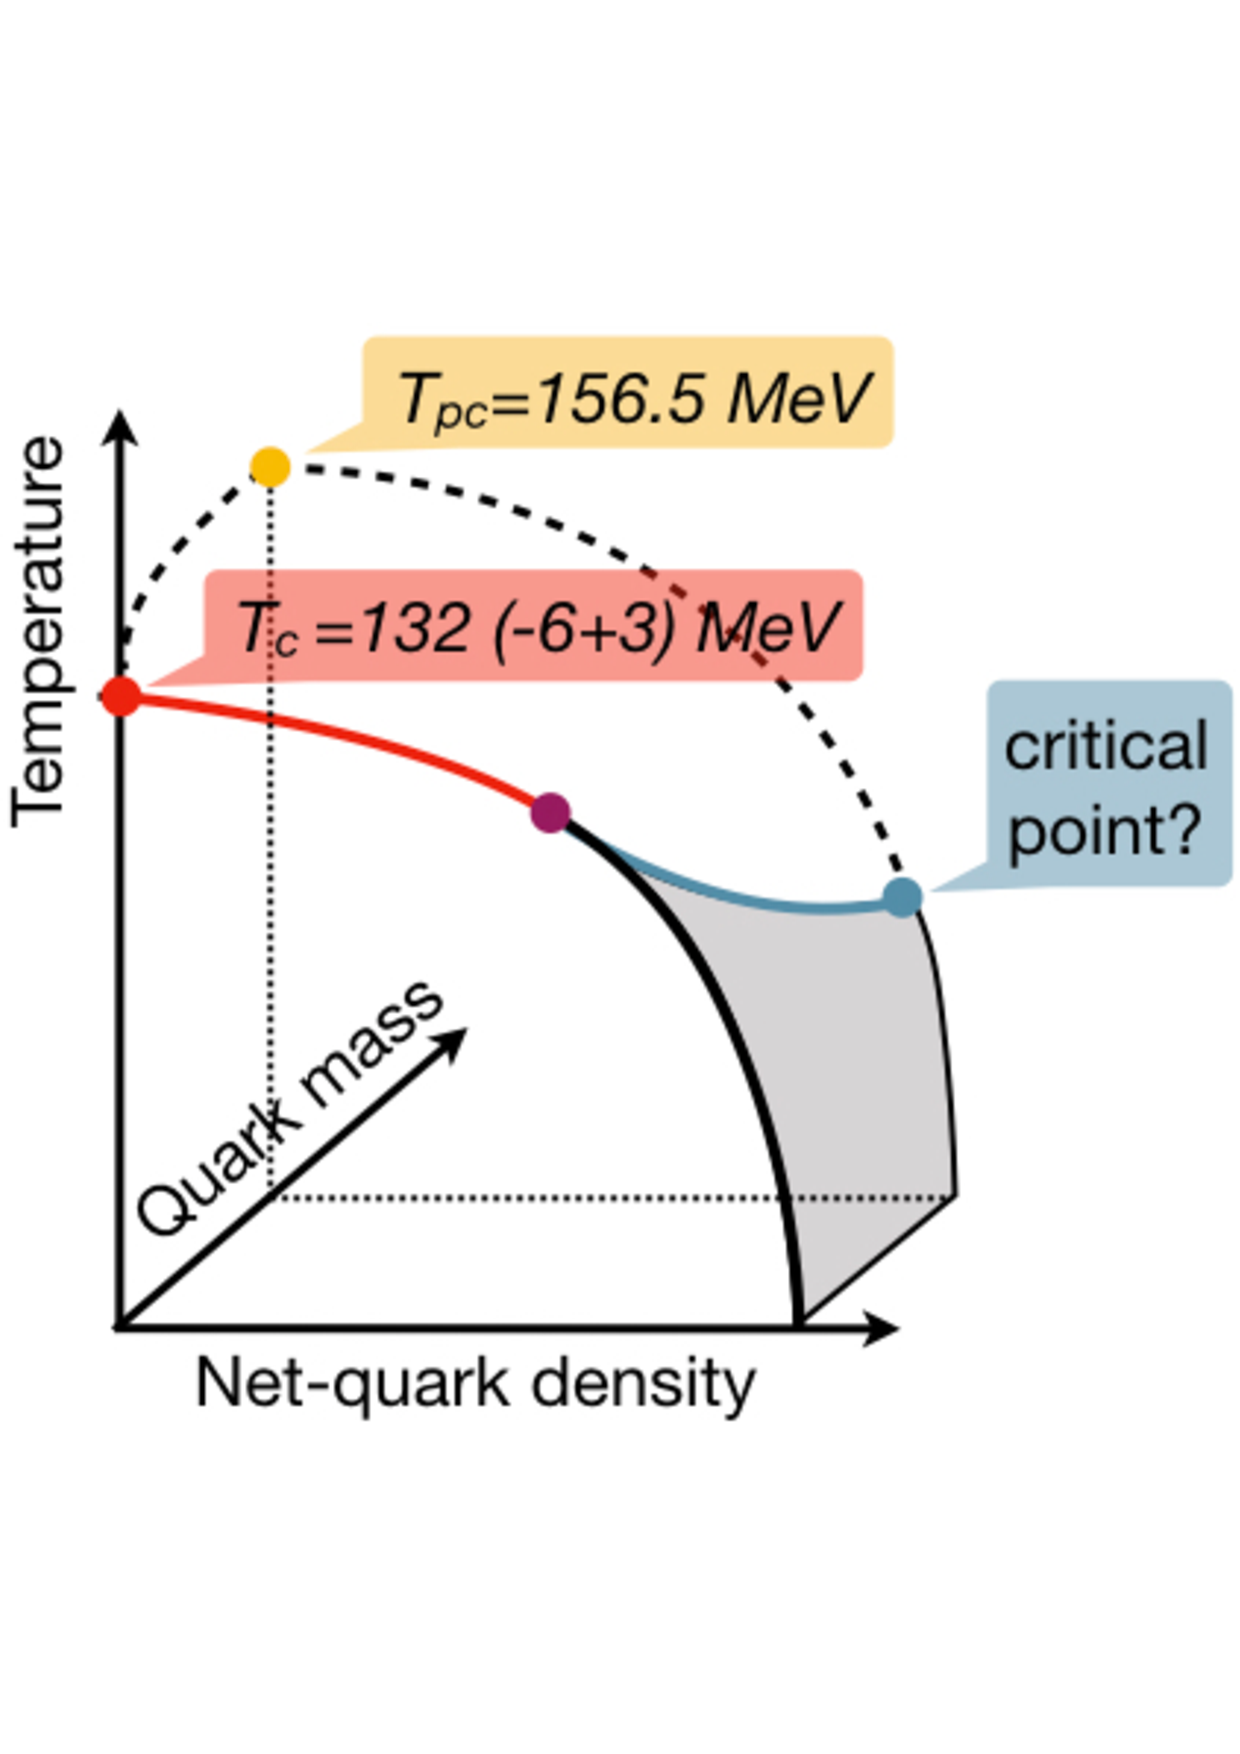
\includegraphics[width=0.6\linewidth]{figs/3d_phase_diag_Gauss.003.pdf}
\vspace{-1cm}
\caption{Schematic phase diagram of QCD. Indicated are the pseudocritical 
transition temperature $\Tpc$ of QCD at physical quark mass and the critical 
transition temperature $\Tc$ in the chiral limit. Dashed lines indicate 
crossovers; thick, solid, colored lines are lines of second-order phase 
transitions; the thick, solid, black line is a line of first-order
transitions; and a first-order surface is indicated in grey. 
A possible critical endpoint is indicated in teal. Figure by C. Schmidt.
This figure is described in some detail in Ref.~\cite{karsch_critical_2019}.}
\label{fig:pdiag}
\end{figure}

At sufficiently high $T$ and/or $\mu_B$, nucleons dissociate into their constituents, 
and nuclear matter changes phase from a gas of hadrons to quark-gluon plasma.
At low enough temperature, one eventually encounters with increasing $\mu_B$ a line of 
first-order transitions, which is expected to terminate at a second-order critical 
endpoint belonging to the 3-$d$, $\Z_2$ universality class, as shown in the rear 
plane of Fig.~\ref{fig:pdiag}.

Let us discuss the qualitative form of the phase diagram in a bit more 
detail~\cite{halasz_phase_1998}.
At $T=0$ and physical quark masses\footnote{We are moving along the dotted,
horizontal line in the rear plane.}, it can be argued that baryon-number 
density $n_B$ should jump at
$\mu\approx m_p$ to the {\it nuclear matter density}\index{nuclear matter
density} $n_0\approx 0.16$ fm$^{-3}$. This jump is discontinuous, and
so the expectation is that transition is first-order, with $n_B$
playing the role of an order parameter.
At sufficiently large $\mu$, color interactions are expected to be screened,
and hence non-perturbative effects like global symmetry breaking should
be suppressed. So for massless quarks, one expects for large $\mu$
a chirally-restored phase, and this should also be of 
first-order\footnote{Now moving along the horizontal axis in
the foreground.}. 
When $\mu$ is sufficiently small and when $m_l=0$,
there is a second-order chiral phase transition belonging to the
$\SU(2)_L\times\SU(2)_R\cong\ON(4)$ universality class.

Returning to the first-order transition at $T=0$ and $m_l=0$,
moving off the $T=0$ axis, continuity demands
the first-order transition to continue as a line. Once $T\neq0$, there
is no longer a well-defined order parameter, and this requirement is lost;
the expectation is this terminates in a tricritical point, which is
itself connect to a second-order line. The ``wings" of this tricritical
point branch off to second-order lines at positive and negative quark
mass\footnote{There is a $m_l\to-m_l$ symmetry, which is not indicated
in the figure since only $m_l\geq0$ is shown.}.

Let us now think about how to probe this diagram on the lattice.
When viewed from the plane of complex $\muh$, the Taylor expansion 
approach is limited by the location of the nearest zero of the QCD partition 
function $\ZQCD$, i.e. the nearest singularity of the free energy in the 
complex plane. In terms of the universal scaling in the vicinity of a critical 
point, the nearest singularity might be identified with the Lee-Yang 
edge, as discussed in \secref{sec:leeyang}. Thus understanding the analytic 
structure of the $\log\ZQCD$ gives crucial insight on both
the convergence radius of these $\muh$-expansions and universal critical behaviour 
in the vicinity of the phase transitions.


\subsection{The sign problem}\index{sign problem}


Unfortunately at $\mu_B>0$, the Boltzmann factor becomes complex, and a 
direct estimate of the path 
integral through MCMC is no longer possible--this is the infamous {\it sign problem}.
This limitation is a special hindrance when looking out for the possible critical 
endpoint at nonzero $\mu_B$ mentioned above. 
Nevertheless many approaches have been developed to at least partially circumvent this limitation, 
each with its own merits, drawbacks, and regions of applicability.
Two popular approaches include Taylor expansions of the equation of state in 
$\muh\equiv\mu_B/T$~\cite{Allton:2002zi, Allton:2003vx, Gavai:2003mf} and analytic continuation 
from purely imaginary chemical potential  $\muh=i\muh_I$~\cite{deForcrand:2002hgr, DElia:2002tig}.

Let us try to understand this problem in more detail.
Most\footnote{Dirac operators with a $\theta$ angle, a twisted mass,
or as we shall shortly see, a chemical potential, lose this property.} 
commonly used Dirac operators $D$ are
$\gamma_5$-{\it hermitian}\index{hermitian}, i.e. they satisfy
\begin{equation}
\gamma_5 D\gamma_5=D^\dagger.
\end{equation}
We already know that hermitian matrices have real eigenvalues, which
is a reason why we like them. 
\begin{proposition}{}{}
Eigenvalues of $\gamma_5$-hermitian matrices come in complex-conjugate pairs.
Moreover their determinants are real.
\begin{proof}
Let $D$ be $\gamma_5$-hermitian. Then since $\gamma_5^2=\id$,
\begin{equation*}\begin{aligned}
\det\left(D-\lambda\id\right)
&=\det\left(\gamma_5^2\left(D-\lambda\id\right)\right)\\
&=\det\left(\gamma_5\left(D-\lambda\id\right)\gamma_5\right)\\
&=\det\left(D^\dagger-\lambda\id\right)\\
&=\det\left(D-\lambda^*\id\right)^*,\\
\end{aligned}\end{equation*}
which shows the first statement. The next statement uses basically
the same trick, i.e.
$$
\det D 
= \det\left(\gamma_5^2 D\right) 
= \det\left(\gamma_5 D\gamma_5\right) 
= \det D^\dagger
= \det D^*.
$$
\end{proof}
\end{proposition}

These kinds of tricks let us see one way the sign problem manifests.
When we introduce a chemical potential, it couples to $\gamma_4$.
Thus a Dirac operator with a chemical potential obeys
\begin{equation}\label{eq:signproblem}
\det\left(D-\mu\gamma_4\right)
=\det\left(\gamma_5\left(D-\mu\gamma_4\right)\gamma_5\right)
=\det\left(D+\mu^*\gamma_4\right)^*
\end{equation}
from which it follows that
$\det\left(D-\mu\gamma_4\right)\in\R$ if and only if $\mu$
is pure imaginary. Hence at real $\mu$, the determinant
is complex. On the other hand, the determinant of the
Dirac operator is part of the probability weight
of the partition function, which one sees explicitly for
the HISQ action in \equatref{eq:HISQdist}. If this
determinant is not strictly real, its interpretation
as a PDF becomes nonsensical.

There is no complete solution to the sign problem. Still, there are
some workarounds that enjoy various degrees of success.
One of the most straightforward is hinted at by
\equatref{eq:signproblem}; namely there is no sign problem
if we simulate at pure imaginary $\mu$. Under the assumption
that we simulate within the convergence radius of our
observable of interest, we can then in principle analytically
continue from the imaginary axis to the real one.

{\it Reweighting}~\cite{ferrenberg_new_1989}\index{reweighting}
is another possibility. Consider
the expectation value of an observable $X$ calculated at $\mu'$. We have
\begin{equation}\label{eq:RW}
\begin{aligned}
  \ev{X}_{\beta'}&=Z_{\beta'}^{-1}\int\dd{\phi}e^{-\beta'E(\phi)}X(\phi)
                  e^{(\beta-\beta)E(\phi)}\\
                 &=Z_{\beta'}^{-1}\int\dd{\phi}e^{(\beta-\beta')E(\phi)}
                  X(\phi)e^{-\beta E(\phi)}\\
                 &=Z_{\beta'}^{-1}Z_{\beta}\ev{e^{(\beta-\beta')E}X}_\beta\\
                 &=\ev{\frac{Z_\beta}{Z_{\beta'}}e^{(\beta-\beta')E}X}_\beta.
\end{aligned}
\end{equation}
We can calculate the expectation value in the last line
using data from a time series generated at $\beta$, and this gives us an
estimate for $\ev{X}_{\beta'}$. Reweighting is only useful when
$E\Delta\beta=\order{1}$. Since $E$ is extensive, this leads to the
expectation that the range of $\beta$ where reweighting gives reliable
information is suppressed for large volumes. 
Provided that the critical parameter $\beta_c$
is sufficiently close to the simulation point $\beta$, it suffices
to have only one simulation, estimating the maximum by reweighting to
multiple nearby $\beta'$. This strategy can be similarly applied
to a chemical potential $\mu$, but the limitation is the same: as
the volume increases the range where one can extract reliable
information gets squeezed.

The Taylor series approach introduced earlier can also be used to
glean some information at $\mu_B>0$. The idea here is that each
coefficient of the Taylor series is by definition computed at
$\mu_B=0$, which can be handled on the lattice. Then assuming
$\mu_B/T$ is small enough, the expansion of some observable in
$\mu_B/T$ ought to be a reasonable approximation.

\index{Roberge-Weiss transition}
\subsection{The Roberge-Weiss transition}\label{sec:RW}



\section{The muon anomalous magnetic moment}\label{sec:muonAnom}

This chapter focuses on some phenomenology I worked on as a postdoc at Utah.
An overview of lattice and dispersive approaches to this problem can
be found in, e.g., Ref.~\cite{aoyama_anomalous_2020}.

The motivation to study the muon anomalous magnetic moment is pretty
straightforward: Observations such as the existence of dark matter and
dark energy cannot be explained by any SM phenomena. One possibility to probe
for new physics is to increase the energy of particle accelerators, thereby
allowing experiment to access higher and higher masses--this is sometimes
called the\index{energy frontier} {\it energy frontier}.
Another possibility is to make more precise measurements, thereby revealing or
sharpening tensions between the SM and experiment--this is
the\index{intensity frontier} {\it intensity frontier}.

As already mentioned in \secref{sec:magAnom}, there is an interesting situation
where data-driven theory exhibit a mild tension with lattice results.
A strategy currently taken by the community to unravel this tension is to
implement modified observables that reduce or magnify systematic effects,
depending on what you want to examine. These are called {\it window observables}
in\index{window observable} the literature.

As an example, the leading HVP contribution $\amuhvp$ in the
{\it time-momentum representation} (TMR) is~\cite{bernecker_vector_2011}
\begin{equation}\label{eq:amuhvp}
  \amuhvp=\left(\frac{\alpha}{\pi}\right)^2\int\dd{t}\tilde{K}(t)G(t),
\end{equation}
where $G(t)$ is the spatially summed correlation function of the EM 
current\footnote{According to the notation of \secref{sec:discreteSymm}
this is a vector current.}
\begin{equation}\begin{aligned}
  G(t) &=-\frac{a^3}{3}\sum_{k=1}^3\sum_{\vec{x}}\ev{j_k(t,\vec{x})j_k(0)},\\
  j_\mu&=\sum_fq_f\bar{\psi}_f\gamma_\mu\psi_f,
\end{aligned}\end{equation}
where $q_f$ is the electric charge of the quark species $f$,
and $\tilde{K}(t)$ is a known kernel function.

In this case a window observable
can be constructed by multiplying the integrand of \equatref{eq:amuhvp} by some
function that enhances the integrand only in certain time windows of the
integral. A step function would naively do the trick, but the authors
in Ref.~\cite{blum_calculation_2018} found that the smoothed step function
\begin{equation}
  \Theta(t,t',\Delta)\equiv\frac{1}{2}\left(1+\tanh\left(\frac{t-t'}{\Delta}\right)\right)
\end{equation}
was somehow less sensitive to discretization effects.
Window observables can be used for high-precision comparisons between both
data-driven calculations and lattice calculations.

\bibliographystyle{unsrtnat}
\bibliography{bibliography}



% Here are the appendices.
\begin{appendices}
\chapter{Special Topic: Misc. Mathematics}\label{ap:spec_math}

This chapter includes some miscellaneous topics in mathematics which are
not long enough to be chapters themselves. Perhaps if any of these sections
were expanded, they could become chapters later, or be incorporated into
other chapters later.


\section{Hyperspherical coordinates}

Here we work out how to compute spherical volumes in $N$ dimensions. 
We warm up with 3D. In 3D we have the radial coordinate
\begin{equation}
  r^2=x^2+y^2+z^2,
\end{equation}
an {\it azimuthal angle} $\phi\in[0,2\pi]$ tracking the projection
on the $x$-$y$ plane, and a {\it polar angle} $\theta\in[0,\pi]$ measuring
the inclination from the $\hat{z}$ direction. 
You can keep from mixing up the
names by thinking of $\theta$ as measuring the distance from the North pole.
The Cartesian coordinates are recovered from the spherical coordinates by
\begin{equation}
  \begin{aligned}
    z&=r\co_\theta\\
    x&=r\s_\theta\co_\phi\\
    y&=r\s_\theta\s_\phi.
  \end{aligned}
\end{equation}
The strange ordering of the coordinates will make sense when we move
to $N$ dimensions. Now the Jacobian corresponding to the transformation between 
Cartesian and spherical coordinates is
\begin{equation}
  \pdv{(x,y,z)}{(r,\theta,\phi)}
  =\left(\begin{array}{ccc}
     \s_\theta\co_\phi & r\co_\theta\co_\phi & -r\s_\theta\s_\phi \\
     \s_\theta\s_\phi  & r\co_\theta\s_\phi  & r\s_\theta\co_\phi \\
     \co_\theta        & -r\s_\theta         & 0                  \\ 
   \end{array}\right).
\end{equation}
Knowing the Jacobian, we compute the volume element
\begin{equation}
  \dd[3]{x}=\det\pdv{(x,y,z)}{(r,\theta,\phi)}
             \dd{r}\dd{\theta}\dd{\phi}
      =r^2\dd{r}\s_\theta\dd{\theta}\dd{\phi}=r^2\dd{r}\dd{\Omega},
\end{equation}
where we will generically use $\dd\Omega$ to stand in for the solid angle,
regardless of the dimension. Integrating over the solid angle gives
\begin{equation}
  \dd{\Omega}=\int_0^{2\pi}\dd{\phi}\int_0^{\pi}\s_\theta\dd{\theta}=4\pi,
\end{equation}
so that the surface area of the 3-ball becomes
\begin{equation}\label{eq:3ds}
  S_3=R^2\int\dd{\Omega}=4\pi R^2,
\end{equation}
and the corresponding volume is
\begin{equation}\label{eq:3dv}
  V_3=\int_0^R\dd{r}r^2\int\dd{\Omega}=\frac{4}{3}\pi R^3.
\end{equation}

Now let us work in $N>3$ dimensions. We define a radial coordinate
\begin{equation}
  r^2=\sum_{i=1}^N x_i^2
\end{equation}
with one azimuthal angle $\phi\in[0,2\pi]$ and $N-2$ polar angles 
$\theta_i\in[0,\pi]$. To see that this mapping covers all of $\R^N$,
note that the azimuthal angle covers an entire 2D plane; then one
only has to sweep the 2D plane from 0 to $\pi$ to cover an entire
3D hyperplane; and continuing in this way fills the entire $N$-dimensional 
volume, because the entire $(N-1)$-dimensional hyperplane was filled out in 
the preceding step. The Cartesian coordinates generalize the pattern
of the 3D case as 
\begin{equation}\label{eq:cartesianN}
  \begin{aligned}
        x_1&=r\co_{\theta_1}\\
        x_2&=r\s_{\theta_1}\co_{\theta_2}\\
     \vdots&\\
    x_{N-2}&=r\s_{\theta_1}...\s_{\theta_{N-3}}\co_{\theta_{N-2}}\\
    x_{N-1}&=r\s_{\theta_1}...\s_{\theta_{N-3}}\s_{\theta_{N-2}}\co_\phi\\
        x_N&=r\s_{\theta_1}...\s_{\theta_{N-3}}\s_{\theta_{N-2}}\s_\phi,
  \end{aligned}
\end{equation}
so that the coordinate we call ``$x_1$" is our new ``$z$" coordinate.

At this step one could find the Jacobian and its determinant, and thus obtain
the new integration measure. Looking at the coordinates~\eqref{eq:cartesianN}
we see the volume element will generically separate as
\begin{equation}
  \dd[N]{x}=r^{N-1}\dd{\Omega},
\end{equation}
where the power $N-1$ is due to the fact that one column of the Jacobian has no
$r$ dependence, because we differentiated with respect to it. Unfortunately
proceeding directly in this manner would require us to explicitly calculate an
$N\times N$ matrix, calculate its determinant, then integrate over the
resulting solid angle, which seems tedious at best.
Thankfully there is a clever way to do this calculation. 

\begin{proposition}{}{nsolida}
The solid angle in $N$ dimensions is
$$
  \int\dd{\Omega}=\frac{2\pi^{N/2}}{\Gamma(N/2)}.
$$
\begin{proof}
  Recall 
  $$
    \int_{-\infty}^\infty\dd{x}e^{-x^2}=\pi^{1/2}.
  $$
  Therefore
  $$ 
    \int\prod_{i=1}^N\dd{x_i}e^{-x_i^2} 
      =\left(\int_{-\infty}^\infty\dd{x}e^{-x^2}\right)^N=\pi^{N/2}.
  $$
  Switching to hyperspherical coordinates, carrying out
  a substitution, and using the definition of the gamma function,
  we can rewrite the LHS of the above as
  \begin{equation*}\begin{aligned}
    \int\prod_{i=1}^N\dd{x_i}e^{-x_i^2}
       &=\int\dd{\Omega}&&\int_0^\infty\dd{r}r^{N-1}e^{-r^2}\\
       &=&&\frac{1}{2}\int_0^\infty\dd{u}u^{N/2-1}e^u\\
       &=&&\frac{1}{2}~\Gamma(N/2).
  \end{aligned}\end{equation*}
  Solving for the solid angle completes the proof. 
\end{proof}
\end{proposition}
With this proposition, the surface area is easily dispatched,
\begin{equation}
  S_N=\frac{2\pi^{N/2}R^{N-1}}{\Gamma(N/2)},
\end{equation}
as is the volume of the $N$-ball,
\begin{equation}
  V_N=\frac{2\pi^{N/2}R^N}{N\Gamma(N/2)}.
\end{equation}
As expected, these formulae agree with \equatref{eq:3ds}
and \eqref{eq:3dv} when $N=3$.

The Jacobian can be used to obtain the integration measure. For $N>3$
dimensions, however, calculating the determinant can be a little
unwieldy. An equivalent way of getting the measure right is to
use wedge products. For example using properties like
$\dd{x_1}\wedge\dd{x_2}=-\dd{x_2}
  \wedge\dd{x_1}$ and $\dd{x_1}\wedge\dd{x_1}=0$, 
one finds very quickly
\begin{equation}
  \dd{x_1}\wedge\dd{x_2}\wedge\dd{x_3}\wedge\dd{x_4}
   =r^3\s_{\theta_1}^2s_{\theta_2} 
     \dd{r}\wedge\dd{\theta_1}\wedge\dd{\theta_2}\wedge\dd{\phi}
\end{equation}
or, as it is usually written,
\begin{equation}
  \dd[4]{x}=r^3\s_{\theta_1}^2s_{\theta_2}
             \dd{r}\dd{\theta_1}\dd{\theta_2}\dd{\phi}.
\end{equation}
Once we know the measure, we can also save ourselves some work
finding the hyperspherical gradient operator. Each factor of the
measure goes to the denominator of one of the terms. Make sure
each denominator has units of length. In the present case, the
gradient operator is read off from the measure to be
\begin{equation}\label{eq:4dgrad}
  \partial=e_r\pdv{r}
   +e_{\theta_1}\frac{1}{r}\pdv{\theta_1}
   +e_{\theta_2}\frac{1}{rs_{\theta_1}}\pdv{\theta_2}
   +e_\phi\frac{1}{rs_{\theta_1}s_{\theta_2}}\pdv{\phi},
\end{equation}
where $e_i$ are unit vectors in direction $i$ and the $\partial$ on
the LHS is meant to represent a vector, while $\partial$s on the RHS
represents just the partial derivative operator.



%\section{Fourier transforms}


\index{Green's function}
\section{Green's functions}
Using Green's functions is a convenient way to solve differential equations.
Here we follow some remarks about Green's functions in
Ref.~\cite{mccomb_renormalization_2004}.

Generically a differential equation can be written as
\begin{equation}\label{eq:diffyq}
  D_t\,x(t) = f(t),
\end{equation}
where $D$ is a linear differential operator, i.e. it can be written as
a linear combination of derivatives with respect to the variable $t$;
$x$ is some differentiable function of $t$; and $f$ is some other
function of $t$. In physical contexts, differential equations are
evolution laws; in the language I have just introduced, they tell you
how some physical observable $x$ changes as the parameter $t$ changes.
The function on the RHS usually plays the role of a force; therefore
\equatref{eq:diffyq} tells you that $f$ induces some kind of response in 
$x$. Maybe the simplest example of a differential equation like this
is Newton's law, which expressed in these symbols looks like
\begin{equation}
  D_t\,x(t)=m\frac{\dd^2}{\dd t^2}x(t) = f(t).
\end{equation}

\begin{figure}
\centering
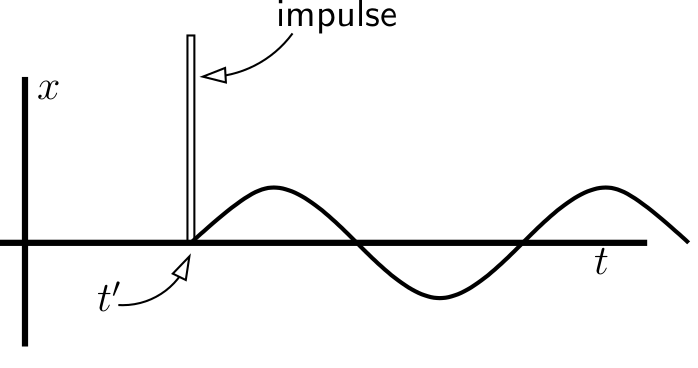
\includegraphics[width=0.44\textwidth]{figs/impulse.png}\\
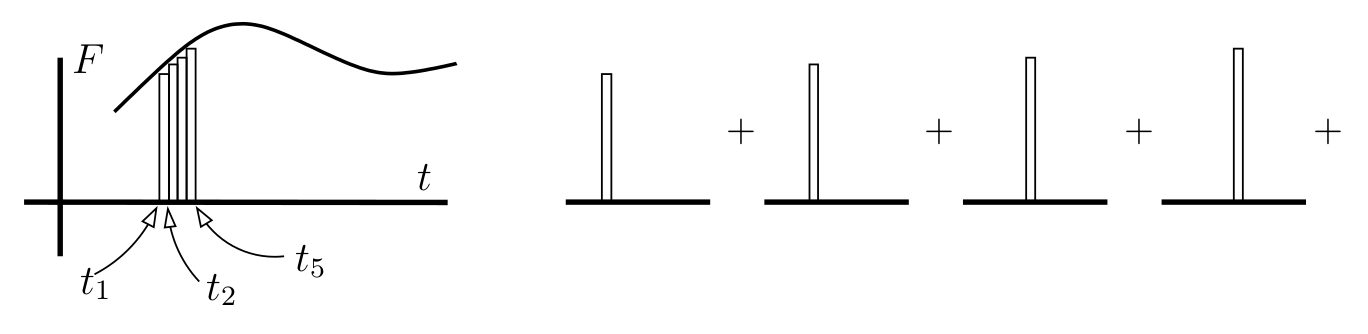
\includegraphics[width=0.90\textwidth]{figs/manyimpulses.png}
\caption{Top: The response of the variable $x$ to a delta function kick at 
$t'$. Bottom: A general force $f$ thought of as the sum of many impulses.
Figure taken from Quintin and Daniel's math methods notes.}
\label{fig:impulse}
\end{figure}

A possibility for $f$ is to use a Dirac delta function
$\delta(t-t')$; in physical contexts, this can be interpreted as a 
kick or {\it impulse}\index{impulse} delivered at time $t'$, and 
the resulting behavior for $x$ is the system's {\it response}\index{response} 
to the kick. This situation is depicted schematically in the top panel of
\figref{fig:impulse}. In such a case, the differential equation
\equatref{eq:diffyq} would become
\begin{equation}\label{eq:greenDelta}
  D_t\,x(t)=\delta(t-t').
\end{equation}
Let's give a special name to the solution of \equatref{eq:greenDelta}: We
are going to call it the {\it Green's function} $G(t-t')$, and it will
therefore satisfy
\begin{equation}\label{eq:greenDeltaSol}
  D_t\,G(t-t')=\delta(t-t').
\end{equation}
But now we are in a position to solve a wide class of differential equations
generally, by taking advantage of the fact that
\begin{equation}\label{eq:deltaSift}
  f(t)=\int\dd{t'}f(t')\delta(t-t').
\end{equation}
One way to interpret the above equation is that this force $f$ is being
constructed from a series of impulses, which is depicted schematically
in the bottom panel of \figref{fig:impulse}. Breaking down the force
in this way, the solution to our general equation \equatref{eq:diffyq} is
\begin{equation}\label{eq:greenSol}
  x(t)=\int\dd{t'}G(t-t')f(t').
\end{equation}
In other words, if we can solve \equatref{eq:greenDelta}, then we can
solve \equatref{eq:diffyq} by using \equatref{eq:greenSol}, almost
regardless of what $f$ is\footnote{I say ``almost" because $f$ must, for
example, be well-behaved enough that the delta function sifting works.}.
Equation~\eqref{eq:greenSol} takes the form of a convolution, and an
intuitive way to look at this convolution is
\begin{equation}
  \text{``output"} = \text{``system response to kicks"} * \text{``input"}.
\end{equation}

In the following two subsections, we are going to solve some
archetypal differential equations using Green's functions. These are
extremely relevant for QFT, and hopefully will help your intuition there.

\index{diffusion equation}
\subsection{The diffusion equation}

We start with a quick reminder about general diffusion equations.
The first core
principle underlying diffusion equations is a conservation law, i.e.
given some generic density $\rho$ depending on $\vec{x}$ and $t$,
\index{continuity equation}
one usually begins with a {\it continuity equation},
\begin{equation}\label{eq:continuityEquation}
  \pdv{\rho}{t}+\nabla\cdot\left(\rho\vec{v}\right)=0,
\end{equation}
where $\vec{v}$ is the velocity of the stuff at position $\vec{x}$. 
To interpret the continuity equation, one thinks about some finite region
in space $V$ and makes use of the divergence theorem to find
\begin{equation}
  \pdv{t}\int_V \dd[3]{x}\rho
     +\int_{S}\dd{\vec{S}}\cdot\left(\rho\vec{v}\right)=0.
\end{equation}
The integral in the first term on the LHS is just the total amount of
stuff enclosed in $V$, while the second term represents the amount of
stuff which is leaving $V$, passing through its surface $S$. In other
words, the continuity equation tells you that rate of change of stuff
in a volume equals the amount of stuff entering it--a formal statement
of an obvious\footnote{Actually while I called this fact obvious,
I guess it is not necessarily. For instance the discovery of mass conservation
is often credited to Antoine Lavoisier, who in the 1770s showed that 
the total mass of a burning system remains unchanged by weighing it
in closed vessels. Before this discovery, the prevailing ``phlogiston"
theory maintained that phlogiston, a conjectured fire-like element,
was released during combustion. Lavoisier was ultimately beheaded
during the French revolution~\cite{wiki:phlogiston,wiki:laviosier}.} fact. 

The second core principle is that when stuff diffuses, it flows from regions
of high concentration to regions of low concentration. This is
sometimes referred to as {\it Fick's law}\index{Fick's law}, and it
can be written as
\begin{equation}\label{eq:ficksLaw}
  \rho\vec{v}+D\nabla\rho=0,
\end{equation}
where $D$ is a constant called the {\it diffusion coefficient}. Combining
\equatref{eq:continuityEquation} and \eqref{eq:ficksLaw}, one finds
\begin{equation}
  \pdv{\rho}{t}-D\nabla^2\rho = 0.
\end{equation}
This is the {\it diffusion equation} in 3+1 dimensions. For the remainder
of this section, to keep the notation light, we will solve the diffusion
equation in 1+1 dimensions.

%\subsection{Perturbation theory}

\section{Dirac algebra}
In this section we summarize Section~3.2 of 
Ref.~\cite{peskin_introduction_1995}.
{\it Gamma matrices} appear when one works with spin-$1/2$ representations of
the Lorentz group. Here we remind the reader of algebraic properties of gamma
matrices. We work in 4D Minkowski space and demand that
\begin{equation}
  \left\{\gamma^\mu,\gamma^\nu\right\}=2g^{\mu\nu}\id,
\end{equation}
where $\id\equiv\id_4$. The representation of the Lorentz algebra is then
\begin{equation}
  S^{\mu\nu}=\frac{i}{4}\left[\gamma^\mu,\gamma^\nu\right].
\end{equation}
An explicit 4D representation of the gamma matrices, called the {\it chiral} 
\index{representation!chiral}\index{representation!Weyl}
or {\it Weyl} representation, uses the Pauli matrices:
\begin{equation}
  \gamma^0=\left(\begin{array}{cc}
                 0      & \id_2    \\
                 \id_2  & 0
           \end{array}\right), \qquad
  \gamma^i=\left(\begin{array}{cc}
                 0         & \sigma^i \\
                 -\sigma^i & 0
           \end{array}\right).
\end{equation}
In this representation, generators of boosts and rotations are, respectively,
\begin{equation}
  S^{0i}=\frac{i}{4}\left[\gamma^0,\gamma^i\right]
        =-\frac{i}{2}
         \left(\begin{array}{cc}
           \sigma^i & 0        \\
           0        & -\sigma^i
         \end{array}\right)
\end{equation}
and
\begin{equation}
  S^{ij}=\frac{i}{4}\left[\gamma^i,\gamma^j\right]
        =\frac{1}{2}\epsilon^{ijk}
         \left(\begin{array}{cc}
           \sigma^k & 0        \\
           0        & \sigma^k
         \end{array}\right).
\end{equation}
A four-component field that transforms under boosts and rotations according to
\index{spinor}
the above generators is called a {\it Dirac spinor}, which we usually denote
with $\psi$. 

Knowing a little bit about gamma matrices, we can introduce
``Feynman slash" notation,\index{slash notation}
\begin{equation}
  \slashed{p}\equiv\gamma_\mu p^\mu,
\end{equation}
and we can then write the {\it Dirac equation} in natural units as
\begin{equation}
  (i\slashed{\partial}-m\id)\psi=0.
\end{equation}
Next we define
\begin{equation}
  \bar{\psi}\equiv\psi^\dagger\gamma^0,
\end{equation}
which allows us to write down the Lorentz scalar $\bar{\psi}\psi$ and
the Lorentz vector $\bar{\psi}\gamma^\mu\psi$. The matrix
\begin{equation}
  \gamma_5=i\gamma^0\gamma^1\gamma^2\gamma^3
\end{equation}
allows us to define left-handed and right-handed projection operators
\begin{equation}\label{eq:projdef}
  P_L\equiv\frac{1}{2}(1-\gamma_5)~~~~\text{and}~~~~
  P_R\equiv\frac{1}{2}(1+\gamma_5),
\end{equation}
which project out the left-handed and right-handed components of Dirac spinors
like
\begin{equation}\label{eq:projact}
  \psi_R=P_R\psi,~~~~
  \psi_L=P_L\psi,~~~~
  \bar{\psi}_R=\bar{\psi}P_L,~~~~\text{and}~~~~
  \bar{\psi}_L=\bar{\psi}P_R.
\end{equation}
The following Propositions tell us how to manipulate gamma matrices and
projection operators.
\begin{proposition}{}{gammatech}
Gamma matrix identities in $4D$:
\begin{center}\begin{tabular}{lrcl}
1. &$\gamma_5^2$ &=& $\id$;\\
2. &$\left\{\gamma^\mu,\gamma_5\right\}$ &=& $\zd$;\\
3. &$\tr\left[\text{odd no. of $\gamma$s}\right]$ &=& $\zd$;\\
4. &$\slashed{a}\slashed{b}$ &=& $-\slashed{b}\slashed{a}-2(ab)\id$;\\
5. &$\tr\gamma^\mu\gamma^\nu$ &=& $-4g^{\mu\nu}\id$;\\
6. &$\gamma_\mu\gamma^\mu$&=& $-4\id$. 
\end{tabular}\end{center}
\end{proposition}
\begin{proposition}{}{projection}
Projection operator identities:
\begin{center}\begin{tabular}{lrcl}
1. & $P_R^2$ &=& $P_R$;\\
2. & $P_L^2$ &=& $P_L$;\\
3. & $\gamma^\mu P_L$ &=& $P_R \gamma^\mu$;\\
4. & $\gamma^\mu P_R$ &=& $P_L \gamma^\mu$.
\end{tabular}\end{center}
\end{proposition}

\bibliographystyle{unsrtnat}
\bibliography{bibliography}

\chapter{Special Topic: Neutrino Oscillations}\label{ap:spec_neutrino}

This chapter summarizes the experiments and observations that led to the belief
that neutrinos have mass. First the solar neutrino problem and early solar
neutrino experiments are discussed. The atmospheric neutrino problem is
discussed. Next the theory behind neutrino oscillations is explained, along
with a possible Standard Model (SM) mechanism giving neutrinos mass. Recent
experiments supporting the neutrino oscillation hypothesis are discussed,
along with future possibilities for neutrino physics research.

Since this chapter was adapted from a project I did as a grad student in 2015,
the experiments are likely not current. Maybe the status of measurements
such as PMNS matrix elements could be updated in the future.

\index{solar neutrino problem}
\section{The solar neutrino problem}

\begin{figure}
  \centering
  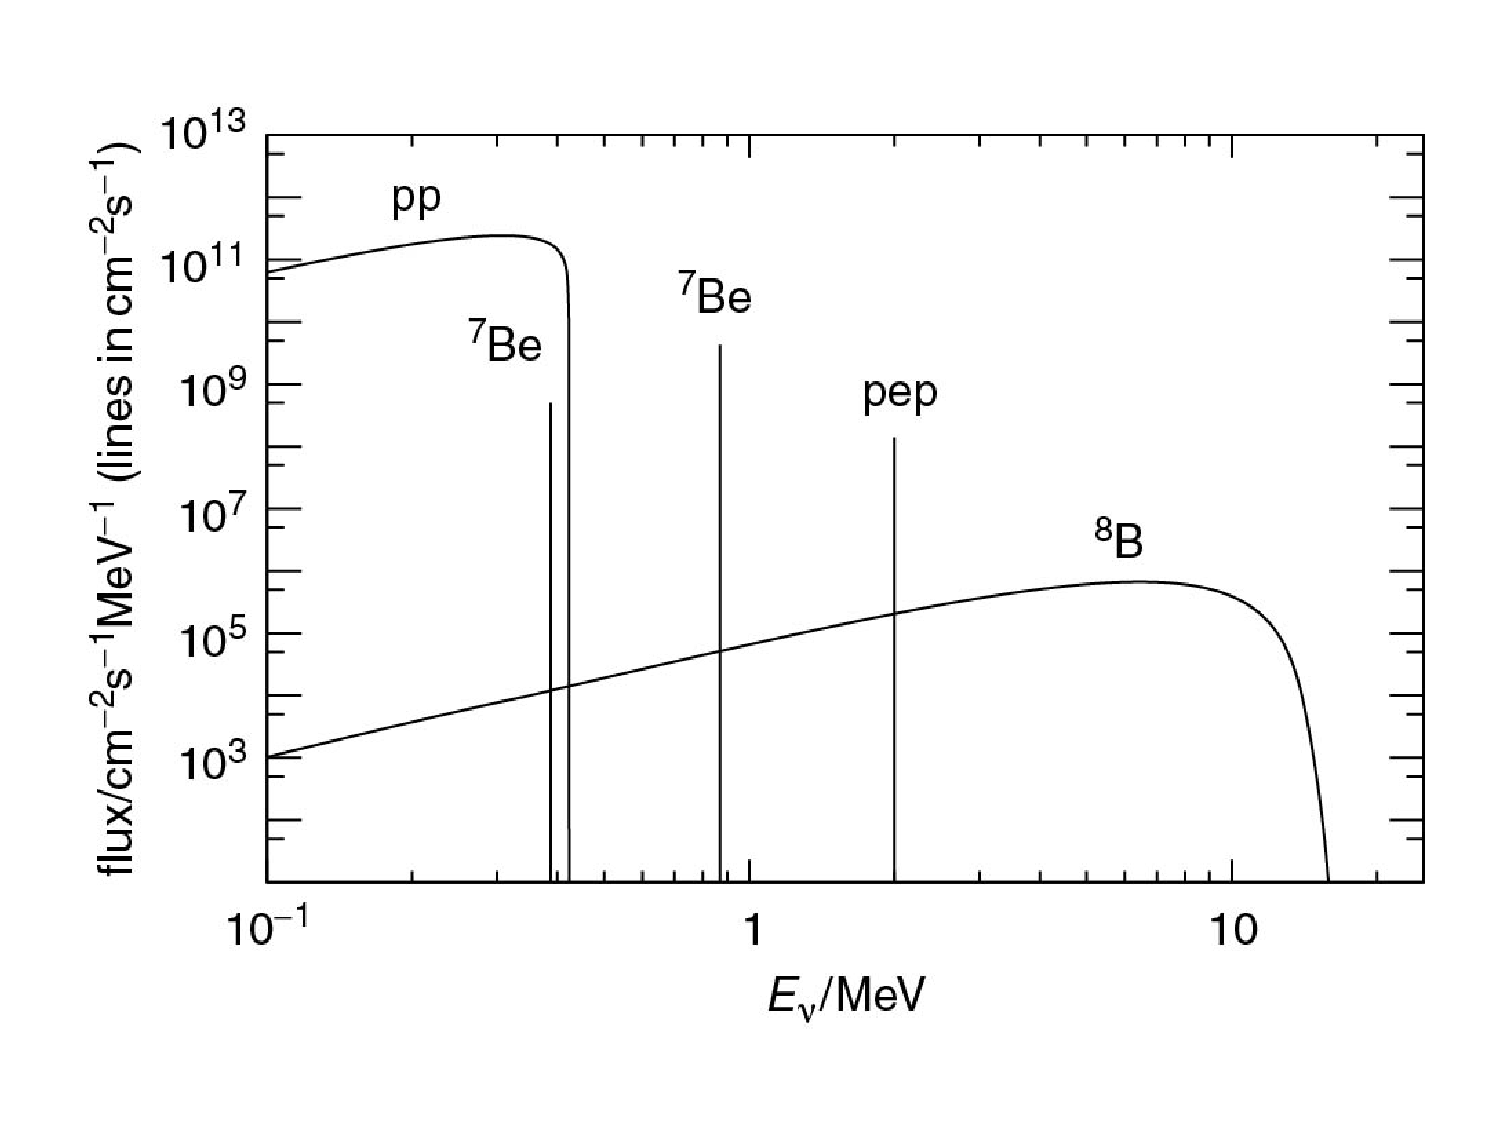
\includegraphics[height=0.33\textheight,keepaspectratio]
                {pictures/t13_3.pdf}
  \caption{Solar neutrino flux and energy of several processes in the sun.
           Image taken from Thomson Fig. 13.3 \cite{thomson_modern_2013}.}
  \label{fig:solar}
\end{figure}
Roughly $2\times10^{38}$ $\nu_e$ are produced by nuclear fusion in the sun
each second. One of the main processes by which this occurs is the pp-cycle,
$\text{p}+\text{p}\to\text{D}+\text{e}^++\nu_e$. However experiments detecting
solar neutrinos tend to focus on rarer reactions, such as the
$\prescript{7}{}{\text{Be}}$ electron capture process, pep-process, and
$\prescript{8}{}{\text{B}}$ $\beta$-decay, which are, respectively,
\begin{equation}
  \begin{aligned}
    \prescript{7}{}{\text{Be}}+\text{e}^-&\to\prescript{7}{}{\text{Li}}+\nu_e,
    \\
    \text{p}+\text{e}^-+\text{p}&\to\prescript{2}{}{\text{H}}+\nu_e, 
    \\
    \prescript{8}{5}{\text{B}}&\to\prescript{8}{4}{\text{Be}}^*+\text{e}^+
      +\nu_e.
  \end{aligned}
\end{equation}
As illustrated in Fig.~\ref{fig:solar}, these processes tend to produce 
neutrinos of higher
energies than the pp-cycle, which allows the neutrinos to overcome kinematic
barriers that would otherwise preclude them from participating in the
interactions used to detect them.
The Standard Solar Model (SSM) allows us to predict how many electron neutrinos
we expect to see. However the results of the first experiments measuring solar
neutrino flux were somewhat unexpected.

\subsection{Radiochemical experiments}
Ray Davis, Jr. and his collaborators started the first experiment to detect
solar neutrinos. The Homestake experiment, based in a mine in South Dakota,
had a 615 ton tank full of dry-cleaning fluid, $\text{C}_2\text{Cl}_4$,
which was chosen for the interaction mentioned below.
Mines are prime real estate for neutrino experiments because being underground
helps isolate them from cosmic rays. The number of captured solar neutrinos
was measured by counting the $\prescript{37}{}{\text{Ar}}$ atoms produced in
the process
\begin{equation}
  \nu_e+\prescript{37}{17}{\text{Cl}}\to
        \prescript{37}{18}{\text{Ar}}+\text{e}^-.
\end{equation}
The minimum energy an electron neutrino needs to participate in the above
process is about 0.81 MeV, which excludes neutrinos produced by the pp-cycle.
Although a huge number of electron neutrinos exit the sun, the SSM
predicted a modest 1.7 interactions per day. The findings
of Homestake were presented in 1968: Merely $0.48\pm0.04$ daily interactions
were found!

Later radiochemical experiments used gallium as a target, and were therefore
sensitive to neutrinos produced in the pp-cycle. The Soviet-American
Gallium Experiment (SAGE) started running in 1989, and appears to still be
collecting data as of March 2015 \cite{gavrin_current_2015}. 
The Gallium Experiment (GALLEX),
which was later succeeded by the Gallium Neutrino Observatory (GNO),
collected data between 1991 and 1997, and was an international project
managed by American, French, German, Italian, Israeli, and Polish scientists.
Both of these experiments confirmed the deficit of solar neutrinos; this
mysterious absence of solar neutrinos became known as the {\it solar
neutrino problem}.

\subsection{Water \v{C}erenkov experiments}
\index{radiation!\v{C}erenkov}
\v{C}erenkov radiation occurs whenever a charged particle passes through a
dielectric medium at a speed greater than the phase speed of light in that
medium. The particle polarizes the medium, then travels away from that
disturbance faster than the electromagnetic field can react, leaving
a wake where those disturbances constructively interfere. Elementary
geometry shows that if the medium has index of refraction $n$, the angle
at which this radiation is emitted is given by $\co=1/n\beta$. Water
\v{C}erenkov detectors work by measuring this angle as leptons propagate
through water. This in turn gives a measure of $\beta$, and hence the energy.
A schematic of a \v{C}erenkov ring is given in Fig. \ref{fig:cerenkov} (b).

\begin{figure}
  \centering
  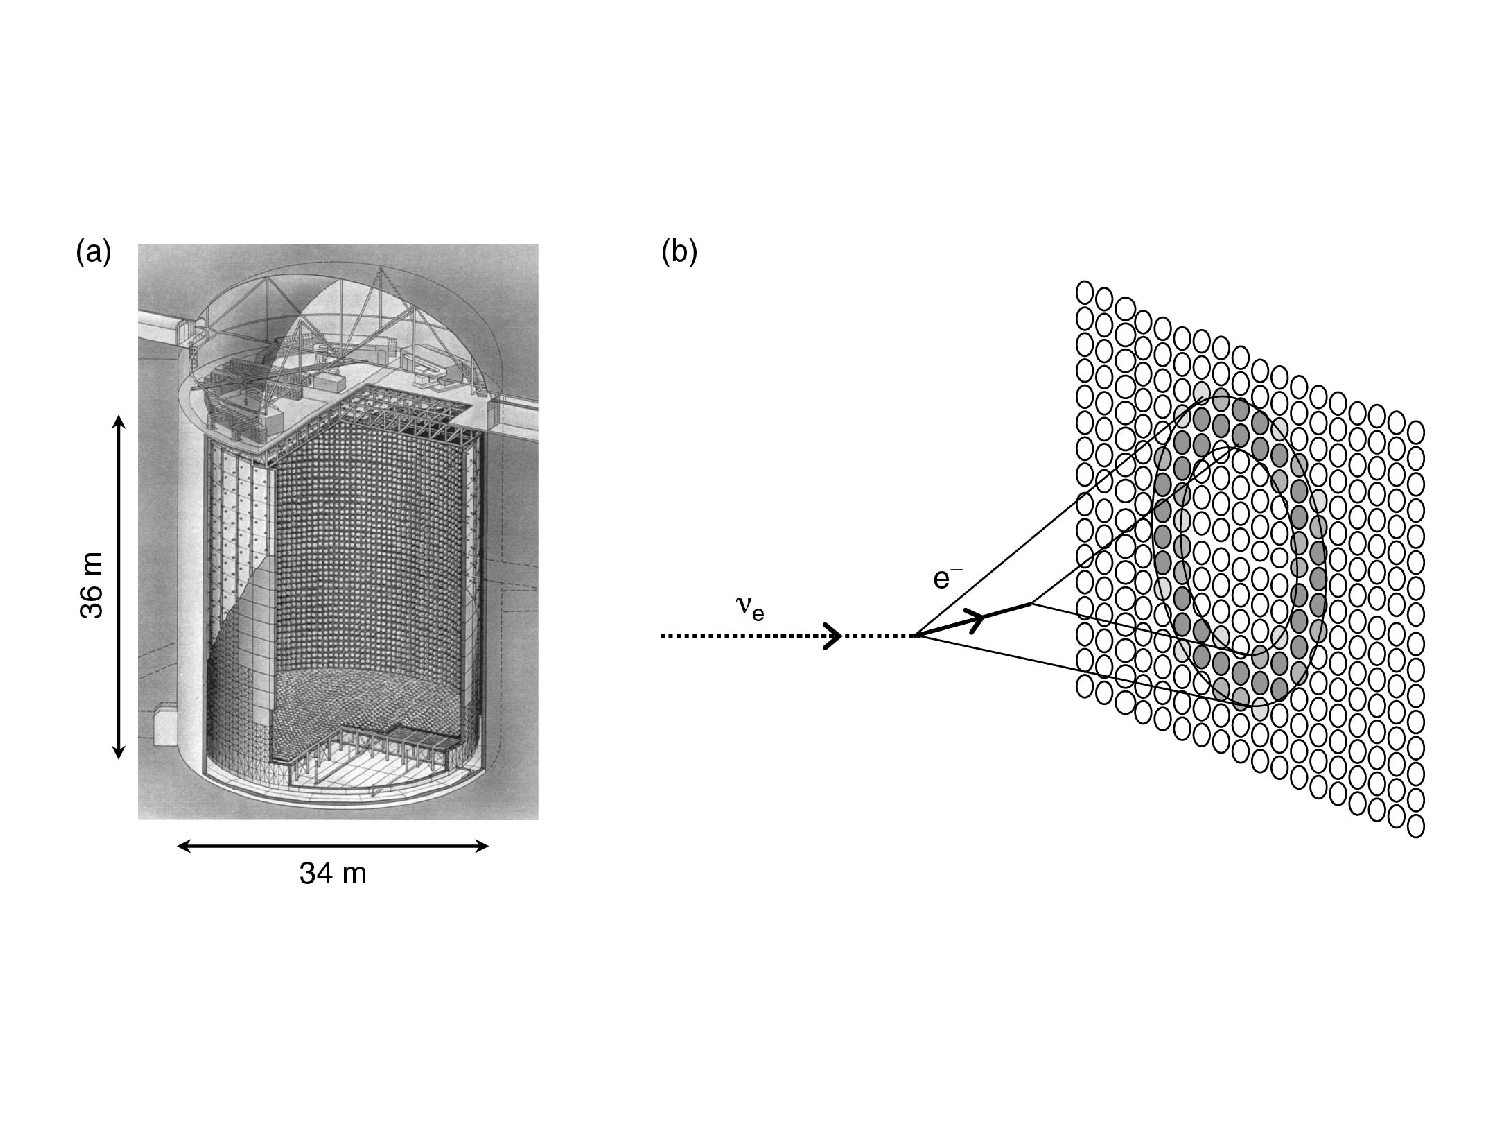
\includegraphics[width=0.75\textwidth,keepaspectratio]
                {pictures/t13_4.pdf}
  \vspace{-10mm}
  \caption{(a) Schematic of the Super-K tank. (b) Electron
           projecting a \v{C}erenkov ring on PMTs. Image taken
           from Thomson Fig. 13.4 \cite{thomson_modern_2013}.}
  \label{fig:cerenkov}
\end{figure}

The Kamioka Nucleon Decay Experiment (or Kamiokande) was
originally a project to study proton decay. In 1988 it was
upgraded, giving it the ability to study solar neutrinos. It was upgraded
again in 1996, donning the name Super Kamiokande (Super-K), with the intent
of obtaining higher statistics than Kamiokande. Super-K is still running today.
Located 1 km underground in the Kamioka area of Gifa Prefecture, Japan,
the Super-K detector consists of a 50 kiloton water tank viewed by 11,146
photo multiplier tubes (PMTs). As charged leptons pass through the water,
they project rings of \v{C}erenkov light on the walls of the detector. The
center-of-mass (CM)
frame is boosted in the direction of the neutrino, which means that the
electron direction is very close to the neutrino direction. This setup
allows experimentalists to not only detect neutrino energies down to
approximately 5 MeV, but also detect particle orientations, which gives Super-K
an advantage over radiochemical experiments. A schematic of this setup
is shown in Fig. \ref{fig:cerenkov} (a).
The neutrinos are detected through the elastic scattering (ES) process
$\nu_ee^-\to\nu_ee^-$. One might expect to also see neutrinos interact
using oxygen, in particular through the charged current (CC) process
$\nu_e+\prescript{16}{8}{\text{O}}\to\prescript{16}{9}{\text{F}}+e^-$.
But oxygen is more stable than the fluorine isotope, making the process
kinematically forbidden to the relatively low energy solar neutrinos. The 5
MeV threshold, which is a result of radioisotope $\beta$ decay background,
 makes Super-K primarily sensitive to neutrinos produced by
the $\prescript{8}{}{\text{B}}$ process.

The left plot of Fig. \ref{fig:superKdata} is a graph of the electron 
direction with respect to the
direction of the sun. The largest number of events occurred near 
$\co_{\theta_{\rm sun}}=1$,
which provides strong evidence that a large flux of neutrinos comes from the
sun. Just as its predecessors, Super-K experienced an electron neutrino
deficit, finding only $0.474\pm0.03$ of the number of electron neutrinos
predicted by the SSM.

\begin{figure}
  \centering
  \vspace{-20mm}
  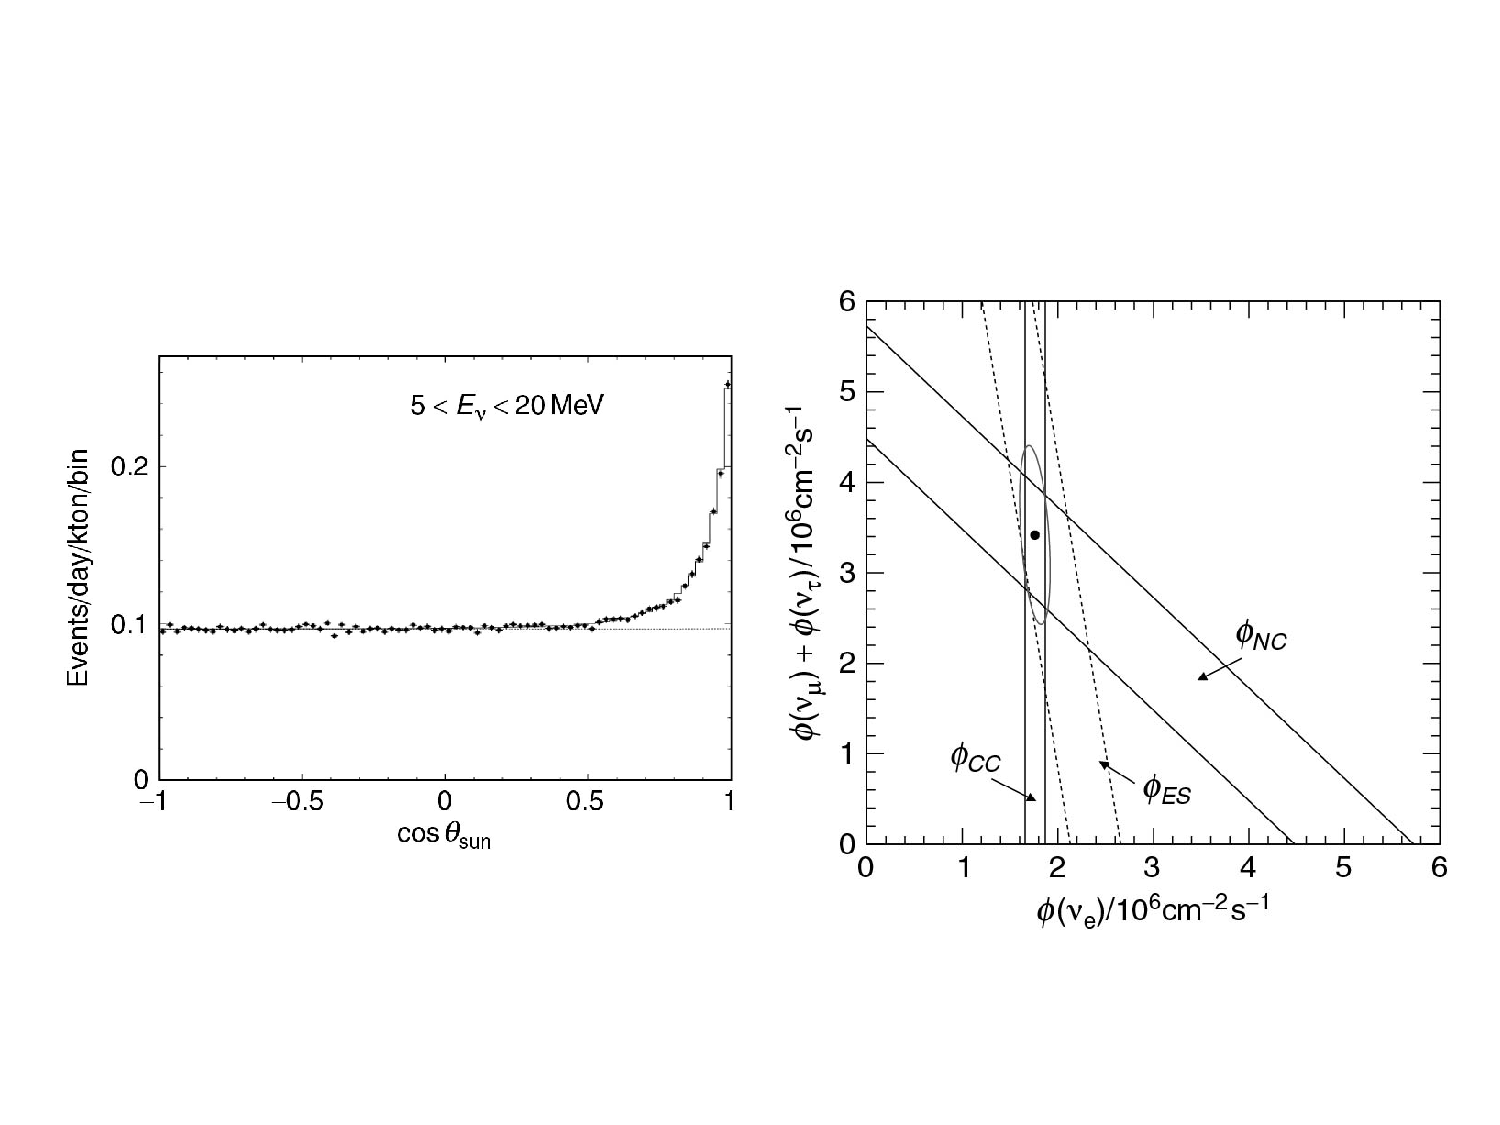
\includegraphics[width=0.9\textwidth,keepaspectratio]
                {pictures/t13_6&8.pdf}
  \vspace*{-20mm}
  \caption{Left: Super-K neutrino data plotted against the cosine of the
           angle of the electron with respect to the sun. Right: Constraints
           on neutrino fluxes from SNO data. The bands indicate one standard
           deviation, and the 68\% confidence ellipse is shown. Images taken
           from Thomson Fig. 13.6 and 13.8 \cite{thomson_modern_2013}.}
  \label{fig:superKdata}
\end{figure}

Homestake, Super-K, and other neutrino experiments demonstrated
a dearth of solar electron neutrinos. The Sudbury Neutrino Observatory (SNO)
in Canada took these experiments a step further by measuring the
electron neutrino flux and total neutrino flux from the sun. SNO had a 12m
diameter tank filled with 1 kiloton of $\text{D}_2\text{O}$, which was used
because deuteron has a small binding energy compared to the energies of
neutrinos produced by $\prescript{8}{}{\text{B}}$. Electron neutrinos can then
be detected through
$\nu_e+\text{D}\to\text{e}^-+\text{p}+\text{p}$,
the CC interaction, and neutrinos of all flavors
interact with the deuteron via the neutral current (NC) interaction
$\nu_\ell+\text{D}\to\nu_\ell+\text{n}+\text{p}$ and ES interactions. The NC
interaction is equally sensitive to all flavors of neutrino, but the ES
interaction is more sensitive to electron neutrinos because $\nu_\mu$ and
$\nu_\tau$ only interact through the NC ES process. In total the interaction
rates obey
\begin{equation}
  \begin{aligned}
    \text{CC rate}&\propto\Phi(\nu_e), \\
    \text{NC rate}&\propto\Phi(\nu_e)+\Phi(\nu_\mu)+\Phi(\nu_\tau), \\
    \text{ES rate}&\propto\Phi(\nu_e)+0.154\big(\Phi(\nu_e)+\Phi(\nu_e)\big).
  \end{aligned}
\end{equation}

For the CC interaction, the
emitted electron is detected by its \v{C}erenkov ring. In the CM frame
the direction of the neutrino relative to the electron is nearly isotropic, and
because the neutrino energy is much smaller than the deuteron mass, the
electron orientation is essentially uncorrelated with the sun's direction.
The ES interaction is also detected through \v{C}erenkov rings, but these
leptons correlate with the sun's direction as in the Super-K. For the NC
interaction, the produced neutron is eventually captured in the process
$\text{n}+\prescript{2}{1}{\text{H}}\to\prescript{3}{1}{\text{H}}+\gamma$.
The photon then produces electrons through subsequent interactions that are
then detected by \v{C}erenkov rings. Ultimately SNO found
\begin{equation}
  \begin{aligned}
    \Phi(\nu_e)&=(1.76\pm0.10)\times10^{-6}~\text{cm}^{-2}\text{s}^{-2} \\
    \Phi(\nu_\mu)+\Phi(\nu_\tau)
               &=(3.41\pm0.63)\times10^{-6}~\text{cm}^{-2}\text{s}^{-2},
  \end{aligned}
\end{equation}
The theoretical prediction of the electron neutrino flux was
\begin{equation}
  \Phi(\nu_e)_{\rm theory}
    =(5.1\pm0.9)\times10^{-6}~\text{cm}^{-2}\text{s}^{-1}, 
\end{equation}
so we see that 
$\Phi(\nu_e)_{\rm theory}=\Phi(\nu_e)+\Phi(\nu_\mu)+\Phi(\nu_\tau)$
within error. Thus SNO showed that the total
neutrino flux was consistent with the theoretical expectation as long as
one allows the neutrino flux from the sun to include muon and tau neutrinos.
But these flavors of neutrinos aren't produced in the sun; therefore SNO also
provided real evidence of neutrino oscillations.
A plot showing the confidence bands of the different processes for data
generated by SNO is shown on the right of Fig. \ref{fig:superKdata}.

These early discoveries about neutrinos weren't merely surprising; they
created a new and burgeoning area of study in high energy physics
that lends important
insight to the nature of SM neutrinos. Discoveries about neutrinos tend
to generate a lot of excitement.
In fact in 2002, Ray Davis and Masatoshi Koshiba each received 1/4 of
the Nobel Prize for their involvement in neutrino detection, the former
due to Homestake and the latter due to Super-K. In 2015 
Takaaki Kajita and Arthur B. McDonald split the Nobel Prize for their
stakes in the Super-K and SNO experiments, respectively.

\index{atmospheric neutrino problem}
\section{The atmospheric neutrino problem}
Cosmic rays, which consist mostly of protons and alpha particles, interact with
particles in the earth's atmosphere. Secondary particles emitted in these
interactions will sometimes decay and produce an {\it atmospheric} neutrino,
provided their energy is low enough ($\lesssim2$ GeV). The atmospheric neutrinos
are then produced via
\begin{equation}
  \begin{aligned}
    \text{p}+N&\to\pi^\pm+X, \\
    \pi^\pm&\to\mu^\pm+\nu_\mu(\bar{\nu}_\mu), \\
    \mu^\pm&\to e^\pm+\nu_e(\bar{\nu}_e)+\bar{\nu}_e(\nu_\mu).
  \end{aligned}
\end{equation}
Assuming the neutrino flavor doesn't change on its journey to the detector,
the above sequence of processes implies
\begin{equation}
  \mathcal{R}\equiv\frac{N_{\nu\mu}+N_{\bar{\nu}\mu}}
                           {N_{\nu e}+N_{\bar{\nu}e}}\approx2,
\end{equation}
where $N_i$ indicates the number of particles of type $i$.
It is difficult to determine an exact value for $\mathcal{R}$ because it is
affected by many factors, including solar activity and geomagnetic cut-off.
Therefore to create a quantity independent of external effects, we define
\begin{equation}
  \mathcal{R}'\equiv\frac{\mathcal{R}}{\mathcal{R}_\text{MC}},
\end{equation}
where $\mathcal{R}_\text{MC}$ is obtained using Monte Carlo simulations instead
of observed data. A drawback to $\mathcal{R}'$ is that it cannot distinguish
between an abundance of electrons and a deficit of muons.

In 1986, the first experiment to discover a discrepancy between the number of
observed and expected atmospheric neutrinos was the Irvine-Michigan-Brookhaven
detector (IMB), which was located in a salt mine owned by Morton on 
the shore of Lake
Erie, Ohio.  Shortly thereafter in 1988, Kamiokande confirmed this deficit.
The next two experiments to investigate this phenomenon, Fr\'ejus and NUSEX,
actually were unable to reproduce this finding. As a result many physicists
believed the discrepancy was due to systematic errors originating in our poor
understanding of neutrino interactions with iron and water. The issue was
resolved when the Soudan2 experiment reaffirmed the findings of IMB and
Kamiokande. But the most convincing results came from Super-K, which showed
that the deficit of neutrinos depends on the zenith angle.

\begin{figure}
  \centering
  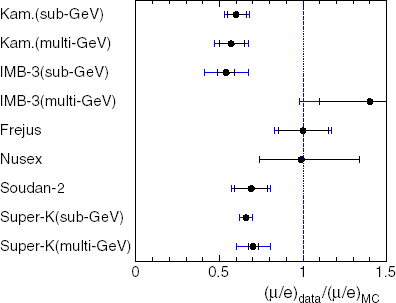
\includegraphics[width=0.85\textwidth,height=0.25\textheight,keepaspectratio]
                {pictures/dblratio.jpg}
  \vspace*{10mm}
  \caption{Plot summarizing the values of $\mathcal{R}'$ as found by early
           neutrino experiments. Image taken from Fig. 11 on T2K experiment
           webpage \cite{T2K}.}
  \label{fig:rprime}
\end{figure}

\index{neutrino!oscillation}
\section{Theory of neutrino oscillations}
Thankfully, both the atmospheric and solar neutrino problems are resolved
neatly by neutrino oscillations.
Here we briefly explain the theory behind neutrino oscillations as well as a
model for how neutrinos gain mass. In the following, we use $x$ to denote
the four-vector of a particle's space-time position.

\index{neutrino!eigenstates}
The {\it mass eigenstates} $\nu_1$, $\nu_2$, and $\nu_3$ of the free particle
Hamiltonian are its physical states of definite mass; i.e., they are the
eigenstates of the Hamiltonian. Meanwhile the {\it weak eigenstates} $\nu_e$,
$\nu_\mu$, and $\nu_\tau$ are the eigenstates corresponding to particles
produced in weak interactions. There is no a priori reason to assume that these
are the same set of eigenstates--in general each set forms a basis spanning
the space of physical states. Hence we can relate the bases to each other
through a unitary transformation, represented below as the
Pontecorvo-Maki-Nakagawa-Sakata (PMNS) matrix. \index{PMNS matrix}We write
\begin{equation}
  \colvec{3}{\nu_e}{\nu_\mu}{\nu_\tau}=
  \left(\begin{array}{ccc}
    U_{e1} & U_{e2} & U_{e3} \\
    U_{\mu 1} & U_{\mu 2} & U_{\mu 3} \\
    U_{\tau 1} & U_{\tau 2} & U_{\tau 3}
  \end{array}\right)
  \colvec{3}{\nu_1}{\nu_2}{\nu_3}
\end{equation}
from which we see that the electron neutrino state, for example, is
a superposition of the mass eigenstates
\begin{equation}
  \label{eq:mix1}
  \ket{\nu_e}=U_{e1}^*\ket{\nu_1}+U_{e2}^*\ket{\nu_2}+U_{e3}^*\ket{\nu_3}.
\end{equation}
Once the neutrino weakly interacts, the wavefunction collapses to a (possibly
different) weak eigenstate. This is believed to be the mechanism by which
neutrinos change flavor.

\index{PMNS matrix}
\subsection{The PMNS matrix}

In general the elements of the PMNS matrix are complex,
so it can be parameterized by eighteen real numbers. However since
$U^\dagger U=\id$, we obtain nine constraints among the elements, which leaves
nine parameters. Hence the matrix can be written in terms of three
mixing angles $\theta_{12}$, $\theta_{23}$, and $\theta_{13}$, and six phases.
Five of these phases can be absorbed in the definitions of neutrino
and charged lepton spinors without modifying weak interaction currents. To
see this note that using the PMNS matrix, a typical weak interaction term can
be written as
\begin{equation}
  -i\frac{g_W}{\sqrt{8}}(\bar{e},\bar{\mu},\bar{\tau})\gamma^\mu(1-\gamma_5)
  \left(\begin{array}{ccc}
    U_{e1} & U_{e2} & U_{e3} \\
    U_{\mu 1} & U_{\mu 2} & U_{\mu 3} \\
    U_{\tau 1} & U_{\tau 2} & U_{\tau 3}
  \end{array}\right)
  \colvec{3}{\nu_1}{\nu_2}{\nu_3}. \\
\end{equation}
We can rephase the PMNS matrix by pulling out two diagonal matrices
of three phases each, one on the left and one on the right. The left matrix
of phases can then be incorporated into the charged lepton phases while the
right matrix of phases is incorporated into the neutrino phases. The reason
that this eliminates five parameters rather than six is that one of these
phases is redundant; indeed, multiplying the PMNS matrix by an overall phase
$\theta$ has no physical consequence, and the other six phases can be
defined relative to $\theta$.

Ultimately we are left with our three angles and one phase, which we will
call $\delta$. The PMNS is then usually cast as something close to a product
of three rotations about orthogonal axes,
\begin{equation}
  \begin{aligned}
    U_{\rm PMNS}&=
    \left(\begin{array}{ccc}
      1 & 0 & 0 \\
      0 & c_{23} & s_{23} \\
      0 & -s_{23} & c_{23}
    \end{array}\right)
    \left(\begin{array}{ccc}
      c_{13} & 0 & s_{13}e^{-i\delta} \\
      0 & 1 & 0 \\
      -s_{13}e^{i\delta} & 0 & c_{13}
    \end{array}\right)
    \left(\begin{array}{ccc}
      c_{12} & s_{12} & 0 \\
      -s_{12} & c_{12} & 0 \\
      0 & 0 & 1
    \end{array}\right)\\
    &=
    \left(\begin{array}{ccc}
      c_{12}c_{13} & s_{12}c_{13} & s_{13}e^{-i\delta} \\
      -s_{12}c_{23}-c_{12}s_{23}s_{13}e^{i\delta} 
       & c_{12}c_{23}-s_{12}s_{23}s_{13}e^{i\delta} & s_{23}c_{13} \\
      s_{12}s_{23}-c_{12}c_{23}s_{13}e^{i\delta} 
       & -c_{12}s_{23}-s_{12}c_{23}s_{13}e^{i\delta} & c_{23}c_{13}
    \end{array}\right),
  \end{aligned}
\end{equation}
where $c_{ij}\equiv \cos\theta_{ij}$ and
$s_{ij}\equiv \sin\theta_{ij}$. As a final note, the above computations
were carried out under the assumption that neutrinos correspond to Dirac
spinors. If they correspond to Majorana spinors, two more degrees of freedom
appear, and we have to multiply the PMNS matrix on the right by a diagonal
matrix with three phases, $\alpha_1/2$, $\alpha_2/2$, and 0.

\subsection{Three flavors}
Let us explore the mechanism behind neutrino oscillation in more detail.
The mass eigenstates propagate as plane waves
\begin{equation}
  \label{eq:evolve1}
  \ket{\nu_i(t)}=\ket{\nu_i}e^{-ip_ix},
\end{equation}
where $1\leq i\leq3$. Suppose that at $x=0$ an electron neutrino
is produced in a weak process and let $\phi_i=p_i~x$. Then from \equatref{eq:mix1} 
and \eqref{eq:evolve1}, the wavefunction at an arbitrary
space-time point $x$ is
\begin{equation}
  \begin{aligned}
    \ket{\psi(x)}&=U_{e1}^*\ket{\nu_1}e^{-i\phi_1}
                  +U_{e2}^*\ket{\nu_2}e^{-i\phi_2}
                  +U_{e3}^*\ket{\nu_3}e^{-i\phi_3} \\
                 &=U_{e1}^*(U_{e1}\ket{\nu_e}+U_{\mu 1}\ket{\nu_\mu}
                   +U_{\tau 1}\ket{\nu_\tau})e^{-i\phi_1} \\
                 &~~~~~~
                  +U_{e2}^*(U_{e2}\ket{\nu_e}+U_{\mu 2}\ket{\nu_\mu}
                   +U_{\tau 2}\ket{\nu_\tau})e^{-i\phi_2} \\
                 &~~~~~~
                  +U_{e3}^*(U_{e3}\ket{\nu_e}+U_{\mu 3}\ket{\nu_\mu}
                   +U_{\tau 3}\ket{\nu_\tau})e^{-i\phi_3} \\
                 &=\left(U_{e1}^*U_{e1}e^{-i\phi_1}
                    +U_{e2}^*U_{e2}e^{-i\phi_2}
                    +U_{e3}^*U_{e3}e^{-i\phi_3}\right)\ket{\nu_e} \\
                 &~~~~~~
                   +\left(U_{e1}^*U_{\mu 1}e^{-i\phi_1}
                    +U_{e2}^*U_{\mu 2}e^{-i\phi_2}
                    +U_{e3}^*U_{\mu 3}e^{-i\phi_3}\right)\ket{\nu_\mu} \\
                 &~~~~~~
                   +\left(U_{e1}^*U_{\tau 1}e^{-i\phi_1}
                    +U_{e2}^*U_{\tau 2}e^{-i\phi_2}
                    +U_{e3}^*U_{\tau 3}e^{-i\phi_3}\right)\ket{\nu_\tau}.
  \end{aligned}
\end{equation}
We can extract oscillation probabilities from the above equation by projecting
the state vector on weak eigenstates. For instance the probability of finding
that our initial electron neutrino has oscillated into a muon neutrino at $x$ is
\begin{equation}
  \pr{\nu_e\to\nu_\mu}=\left|U_{e1}^*U_{\mu 1}e^{-i\phi_1}
                    +U_{e2}^*U_{\mu 2}e^{-i\phi_2}
                    +U_{e3}^*U_{\mu 3}e^{-i\phi_3}\right|^2.
\end{equation}
Using the unitarity relations among the PMNS matrix elements, along with the
identity
\begin{equation}
  |z_1+z_2+z_3|^2=|z_1|^2+|z_2|^2+|z_3|^2
                  +2\Re{z_1z_2^*+z_1z_3^*+z_2z_3^*},
\end{equation}
the above oscillation probability simplifies to
\begin{equation}
  \begin{aligned}
    \pr{\nu_e\to\nu_\mu}=&
    \,2\Re{U_{e1}^*U_{\mu 1}U_{e2}U_{\mu 2}^*\left(e^{i(\phi_2-\phi_1)}-1\right)}
     \\&~+
    2\Re{U_{e1}^*U_{\mu 1}U_{e3}U_{\mu 3}^*\left(e^{i(\phi_3-\phi_1)}-1\right)}
     \\&~+
    2\Re{U_{e2}^*U_{\mu 2}U_{e3}U_{\mu 3}^*\left(e^{i(\phi_3-\phi_2)}-1\right)}
     .
  \end{aligned}
\end{equation}
Similarly the electron neutrino survival probability is
\begin{equation}
  \begin{aligned}
    \pr{\nu_e\to\nu_e}=1&+2|U_{e1}|^2|U_{e2}|^2\Re{e^{i(\phi_2-\phi_1)}-1} \\
                        &+2|U_{e1}|^2|U_{e3}|^2\Re{e^{i(\phi_3-\phi_1)}-1} \\
                        &+2|U_{e2}|^2|U_{e3}|^2\Re{e^{i(\phi_3-\phi_2)}-1}.
  \end{aligned}
\end{equation}
To simplify these equations, define phase differences by
\begin{equation}
  \label{eq:phase}
  \Delta_{ji}\equiv\frac{\phi_j-\phi_i}{2}
                  =\frac{(m_j^2-m_i^2)|\vec{x}|}{4E_\nu}.
\end{equation}
The equality follows from the facts that
\begin{equation}
  \phi_j-\phi_i=(E_j-E_i)t-(|\vec{p}_1|-|\vec{p}_2|)|\vec{x}|
\end{equation}
and $t\approx|\vec{x}|$ since $\beta\approx1$.
Using the phase differences, we can recast the electron survival probability as
\begin{equation}
  \label{eq:esurv}
  \begin{aligned}
    \pr{\nu_e\to\nu_e}=1&-4|U_{e1}|^2|U_{e2}|^2\sin^2\Delta_{21} \\
                        &-4|U_{e1}|^2|U_{e3}|^2\sin^2\Delta_{31} \\
                        &-4|U_{e2}|^2|U_{e3}|^2\sin^2\Delta_{32}.
  \end{aligned}
\end{equation}
We see that when the phase differences are near zero, the survival probability
is close to 1. Since the masses of the neutrinos are small compared to their
energies, the mass differences are also small. This means that the survival
probability is nearly unity, except over large distances, which proffers
an explanation for why these oscillations did not manifest in early neutrino
beam experiments. We also see that if neutrinos are massless and this model is
correct, then there can be no oscillations. Since we have good evidence that
neutrino oscillations occur, and because we also have evidence that this model
accurately describes them, it follows that neutrinos have nonzero,
non-degenerate masses.

\subsection{Two flavors}
The above formalism gives the general treatment of neutrino oscillations
of three flavors, but for the present neutrino data, it is essentially correct
to assume only two flavors \cite{kajita_neutrino_2009}. 
For this reason, we will briefly review two flavor oscillations.

When there are two flavors, the relationship between the mass and weak bases
can be parameterized by a mixing angle $\theta$, which is analogous to the
Cabibbo angle. We have
\begin{equation}
  \colvec{2}{\nu_e}{\nu_\mu}=
  \left(\begin{array}{cc}
    \co_\theta & \s_\theta \\
    -\s_\theta & \co_\theta
  \end{array}\right)
  \colvec{2}{\nu_1}{\nu_2}.
\end{equation}
Again assuming the particle starts off as an electron neutrino at $x=0$, and
following the same procedure as before, we find the wavefunction at a general
space-time point to be
\begin{equation}
  \begin{aligned}
    \ket{\psi(x)}&=\co_\theta(\co_\theta\ket{\nu_e}-\s_\theta\ket{\nu_\mu})
                   e^{-i\phi_1}
                  +\s_\theta(\s_\theta\ket{\nu_e}+\co_\theta\ket{\nu_\mu})
                   e^{-i\phi_2} \\
                 &=e^{-i\phi_1}\left((\co_\theta^2
                        +e^{i\Delta\phi_{12}}\s^2_\theta)\ket{\nu_e}
                        -(1-e^{i\Delta\phi_{12}})
                         \co_\theta\s_\theta\ket{\nu_\mu}\right),
  \end{aligned}
\end{equation}
where $\Delta\phi_{12}\equiv\phi_1-\phi_2$. Projecting the state vector on
the muon state, applying \equatref{eq:phase}, and finally expressing
$|\vec{x}|$ in [km], $\Delta m$ in [eV], and $E_\nu$ in [GeV] gives the
familiar oscillation probability
\begin{equation}
  \pr{\nu_e\to\nu_\mu}=\sin^2(2\theta)\sin^2
                          \left(1.27\frac{\Delta m^2[\text{eV}^2]
                          |\vec{x}|[\text{km}]}{E_\nu[\text{GeV}]}\right).
\end{equation}

\subsection{Neutrino masses}
From the previous discussion, we see that measurements of neutrino oscillations
place no constraint on the overall mass scale. No direct measurement has been
made of neutrino masses. Nevertheless, cosmological measurements suggest
that \cite{thomson_modern_2013}
\begin{equation}
  m_{\nu1}+m_{\nu2}+m_{\nu3}\lesssim1~\text{eV}. 
\end{equation}
From what we can tell,
neutrino masses are much smaller than other fermion masses. Now let
$\Delta m_{ji}=m_{\nu j}-m_{\nu i}$.
Recent oscillation experiments have determined $\Delta m_{21}^2$ and
$|\Delta m_{32}^2|$ and shown that $\Delta m_{21}^2\ll|\Delta m_{32}^2|$.
These experiments have not been able to determine the sign of
$\Delta m_{32}^2$, an issue which has led to the definition of two {\it mass
hierarchies}. \index{neutrino!mass hierarchy}
In the {\it normal} hierarchy, $m_{\nu1}<m_{\nu2}<m_{\nu3}$,
while in the {\it inverted} hierarchy, $m_{\nu3}<m_{\nu1}<m_{\nu2}$. In
either case, it's clear that $|\Delta m_{31}^2|\approx|\Delta m_{32}^2|$.

The current explanation for the disparity between the masses of the neutrinos
and other fermions, and for how neutrinos acquire masses in the
first place, is as follows. Right-handed neutrinos $\nu_R$ do not
participate in any SM interactions, so
there is no evidence for or against their existence. Therefore we can introduce
neutrino masses in the same way as quarks. After spontaneous symmetry breaking
of the Higgs, the mass term for the neutrino looks like
\begin{equation}
  \Lagr_D=-m_D(\bar{\nu}_R\nu_L+\bar{\nu}_L\nu_R).
\end{equation}
If this term is the origin of masses, then right handed neutrinos must exist.
Nevertheless this explanation is not totally satisfactory because neutrino
masses are small compared to the masses of other fermions. So we add
the mass term
\begin{equation}
  \Lagr_M=-\frac{1}{2}M\left(\bar{\nu}^c_R\nu_R+\bar{\nu}_R\nu^c_R\right),
\end{equation}
where $\nu^c=CP\nu=i\gamma^2\gamma^0\nu^*$. $\Lagr_M$ does not violate local
gauge invariance. Similar terms are forbidden for charged leptons because
they allow particle-antiparticle interactions, which violate charge
conservation. This is no contradiction for the neutral neutrino, which may
very well correspond to a Majorana spinor, in which case it is its own
antiparticle anyway.

Now suppose we add to the SM Lagrangian
\begin{equation}
  \begin{aligned}
    \Lagr_{\nu~\text{mass}}&=-\frac{1}{2}\left(m_D\bar{\nu}_L\nu_R
                            +m_D\bar{\nu}^c_R\nu^c_L+M\bar{\nu}^c_R\nu_R\right)
                             +~\text{h.c.}\\
        &=\left(\bar{\nu}_L,\bar{\nu}_R^c\right)
          \left(\begin{array}{cc}
            0 & m_D \\
            m_D & M
          \end{array}\right)
          \colvec{2}{\nu_L^c}{\nu_R}+~\text{h.c.},
  \end{aligned}
\end{equation}
where the h.c. indicates the hermitian conjugate of everything that precedes it.
Following the usual procedure we obtain particle masses by diagonalizing the
above mass matrix. We find mass eigenvalues
\begin{equation}
  m=\frac{1}{2}M\left(1\pm\sqrt{1+\frac{4m_D^2}{M^2}}\right)
                \approx\frac{1}{2}M
                   \pm\frac{1}{2}M\left(1+\frac{2m_D^2}{M^2}\right)
\end{equation}
assuming $m_D\ll M$. This process reveals light and heavy neutrino states with
masses
\begin{equation}
  |m_\nu|\approx\frac{m_D}{M}\qquad\text{and}\qquad m_N\approx M.
\end{equation}
The {\it seesaw mechanism} hypothesizes that $m_D$ is of the same order as the
\index{seesaw mechanism}
other fermions, a feature that we like, and that the observed neutrino mass is
so small because the Majorana mass $M$ is large and suppresses it. There is
currently no direct evidence for the seesaw mechanism, but if neutrinos were
discovered to be Majorana particles, the mechanism would be even more
compelling.

\section{Neutrino experiments}
We will now examine some experiments that confirm neutrino oscillations and
have allowed us to measure parameters in the PMNS matrix.
Two subclasses of neutrino experiments are reactor experiments
and accelerator experiments. In reactor experiments, nuclear fission produces
radioisotopes, which then emit electron neutrinos during $\beta$ decays.
Electron antineutrinos are detected through the process
\begin{equation}
  \label{eq:betadecay}
  \bar{\nu}_e+\text{p}\to\text{e}^++\text{n},
\end{equation}
but they will not be detected if they oscillate to other flavors, because
the neutrino energy will be too small to produce a muon or tau lepton in
the final state. Thus these experiments can only observe the disappearance
of electron antineutrinos. In beam experiments, a highly relativistic
proton beam is fired at a target, which produces a large number of charged
pions, which subsequently decay via
\begin{equation}
  \begin{aligned}
    \pi^-&\to\mu^-+\bar{\nu}_\mu, \\
    \pi^+&\to\mu^++\nu_\mu.
  \end{aligned}
\end{equation}
The neutrinos and antineutrinos follow the direction of the CM frame boost,
which is in the direction of the incoming pion.

To prepare to analyze more neutrino experiments, we calculate the
electron antineutrino survival probability.
The action of the $T$ operator on the process $\nu_\ell\to\nu_{\ell'}$ is
to interchange the labels $\ell$ and $\ell'$, while $CP$ complex conjugates
the elements of the PMNS matrix. From \equatref{eq:esurv} it follows
that $\pr{\nu_e\to\nu_e}=\pr{\bar{\nu}_e\to\bar{\nu}_e}$. Using the fact
that $|\Delta m_{31}^2|\approx|\Delta m_{32}^2|$ and the unitarity relations,
we can then write
\begin{equation}
  \label{eq:prb}
  \begin{aligned}
    {\rm P}_{\rm surv.}&\equiv\pr{\bar{\nu}_e\to\bar{\nu}_e}\\
      &\approx 1-4|U_{e1}|^2|U_{e2}|^2\sin^2\Delta_{21}
              -4|U_{e3}|^2\left(|U_{e1}|^2+|U_{e2}|^2\right)\sin^2\Delta_{32}
       \\ 
      &= 1-c_{13}^4\sin^2(2\theta_{12})
           \sin^2\left(\frac{\Delta m_{21}^2 |\vec{x}|}{4E_{\bar{\nu}}}
           \right) -\sin^2(2\theta_{13})
           \sin^2\left(\frac{\Delta m_{32}^2 |\vec{x}|}{4E_{\bar{\nu}}}
           \right).
  \end{aligned}
\end{equation}
The second sine factor in the last term has a shorter wavelength than the
second sine factor in the second term because of the relative sizes of the
mass differences. The last term therefore dominates at shorter distances,
while the second term dominates at longer distances. Fig. \ref{fig:kamland}
(left) shows a graph of the survival probability assuming a few typical 
parameter values.

\subsection{Reactor experiments}

\begin{figure}
  \centering
  \vspace{-15mm}
  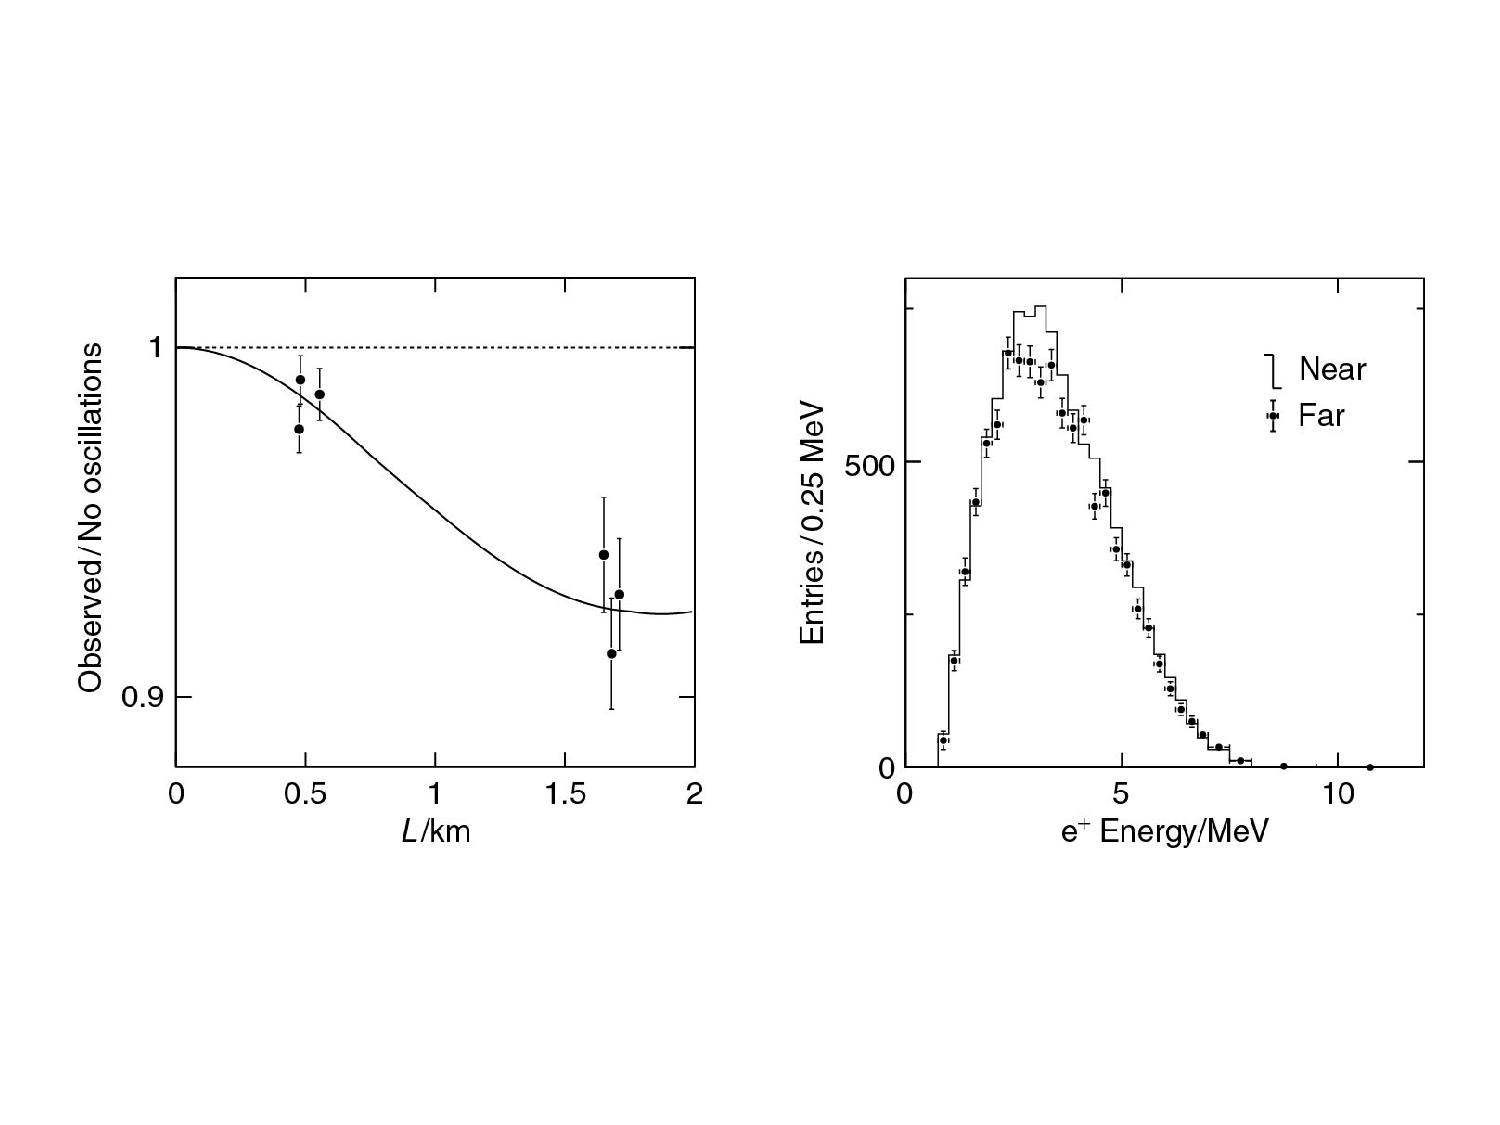
\includegraphics[width=0.9\textwidth,keepaspectratio]
                {pictures/t13_19.pdf}
  \vspace*{-20mm}
  \caption{Left: Daya Bay observed antineutrino rate compared to the
           unoscillated expectation (dotted line). Rates plotted as function
           of flux weighted distance to the reactors (solid line). Right:
           Daya Bay observed near and far e$^+$ energy spectra with the
           background subtracted. Image taken from Thomson Fig. 13.19
           \cite{thomson_modern_2013}.}
  \label{fig:daya}
\end{figure}

\begin{figure}
  \centering
  \vspace{-20mm}
  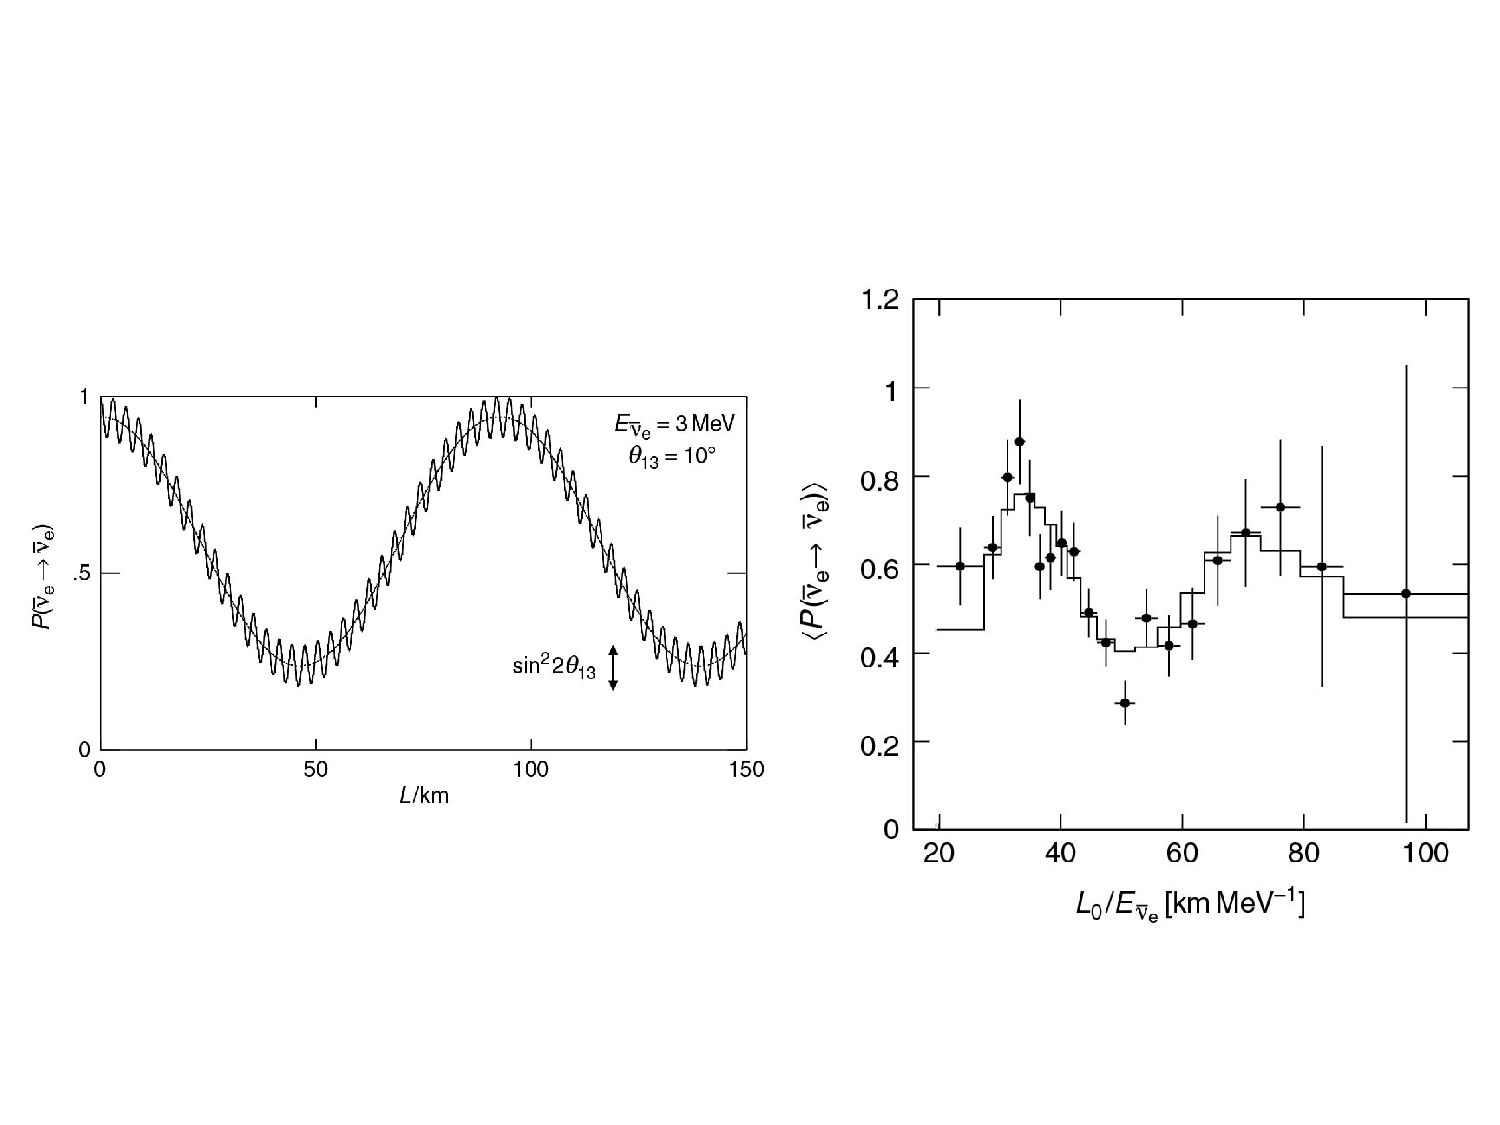
\includegraphics[width=0.9\textwidth,keepaspectratio]
                {pictures/t13_18&20.pdf}
  \vspace*{-15mm}
  \caption{Left: The electron antineutrino survival probability assuming
           $\theta_{12}=12$\textdegree, $\theta_{23}=45$\textdegree,
           $\theta_{13}=10$\textdegree, $\Delta m_{21}^2=8\times10^{-5}$
           $\text{eV}^2$, $\Delta m_{32}^2=2.5\time10^{-3}$ $\text{eV}^2$.
           Right: KamLAND data showing measured mean survival probability.
           The histogram is generated from the expected distribution given
           by the oscillation parameters that best fit the data, taking
           background into account. Images taken from Thomson Fig.
           13.18 and 13.20 \cite{thomson_modern_2013}.}
  \label{fig:kamland}
\end{figure}

The Daya Bay experiment is an international reactor experiment based in China.
It consists of
six nuclear reactors and eight antineutrino detectors placed short, varied
distances (less than 2 km) away from the source. Hence the short
wavelength contribution of \equatref{eq:prb} dominates. Placing the
detectors at different distances allows cancellation of some systematic
uncertainty. The detectors are full of 20 tons of
liquid {\it scintillator}, a material that produces light when it interacts
with a particular particle but doesn't interfere with light itself.
The scintillator is doped with gadolinium and viewed by PMTs, which look for
the process \eqref{eq:betadecay}. Ascertaining whether such an event occurred
involves multiple steps. First the annihilation of the positron with an
electron produces two photons. The neutron scatters in the scintillator until
it is captured by a gadolinium nucleus, which takes roughly 100 $\mu$s and
produces photons. Photons from
the capture and the electron-positron annihilation yield Compton scattered
electrons, which then ionize the scintillator and produce scintillation light.
Hence the experiment counts an inverse beta decay event whenever it detects
a pulse of scintillation light followed by a neutron capture pulse
10-100~$\mu$s later.

The results of the Daya Bay experiment are summarized in Fig. \ref{fig:daya}. 
The left plot compares the observed number of antineutrino events with the
unoscillated hypothesis. There is an unambiguous deviation
that increases with increasing detector distance.
The plot on the right compares the observed e$^+$ energy spectrum in the far
detectors to the spectrum of the near detectors, scaled to the same integrated
neutrino flux. Again the data are consistent with some electron neutrinos
oscillating to other flavors by the time they reach the far detector.
This energy difference then allows a measurement of $\theta_{13}$, and Daya Bay
found \cite{an_observation_2012}
\begin{equation}
  \sin^2(2\theta_{13})=0.092\pm0.016({\rm stat})\pm0.005({\rm sys}).
\end{equation}

The Kamioka Liquid Scintillator Antineutrino Detector (KamLAND) experiment,
located in the same mine as Super-K, consists of two concentric spheres in
water. The inner sphere is full of liquid scintillator and again surrounded by
PMTs, and neutrinos are detected using the same procedure as in Daya Bay.
However instead of gadolinium, the neutron capture occurs through the
process $\bar{\nu}_e+\text{p}\to\text{D}+\gamma$. The detector is situated
130-240 km away from the reactors, so that the long wavelength contribution of
\equatref{eq:prb} is the dominant term. The KamLAND data, depicted in the right
plot of Fig. \ref{fig:kamland}, form a rather nice pattern. 
The plot clearly shows electron
antineutrino survival probabilities that oscillate with $L_0/E_{\bar{\nu}e}$,
where $L_0$ is the flux weighted mean distance from the detector to the
reactors. By comparing this distribution with the long wavelength dominated
survival probability, KamLAND found \cite{abe_precision_2008}
\begin{equation}
  \Delta m_{12}^2=7.58^{+0.14}_{-0.13}({\rm stat})
        \pm0.15({\rm sys})\times10^{-5}~\text{eV}^2.
\end{equation}
KamLAND also determined
\begin{equation}
  \tan^2\theta_{12}=0.56^{+0.10}_{-0.07}({\rm stat})^{+0.10}_{-0.06}({\rm sys}).
\end{equation}

\subsection{Accelerator experiments}
Long baseline accelerator experiments typically have two detectors, one
situated near the source, which reveals the unoscillated neutrino energy
spectrum, and one far away, which reveals the oscillated spectrum.
Many systematic uncertainties cancel when both a near and far detector are
used.
An important accelerator experiment is the Main Injector Neutrino Oscillation
Search (MINOS) at Fermilab. The experiment measures oscillations
of a pure muon neutrino beam. It started collecting data in 2005 and
was upgraded to MINOS+ in 2013. The near detector is situated 1 km
from the source, while the far detector is located in a mine in Minnesota
735 km away. The detectors are made of iron plates with relatively
thin layers of
plastic scintillator. Scintillation light is passed from the scintillator to
PMTs using optical fibers, and the detector is magnetized to measure
muon momentum.

\begin{figure}
  \centering
  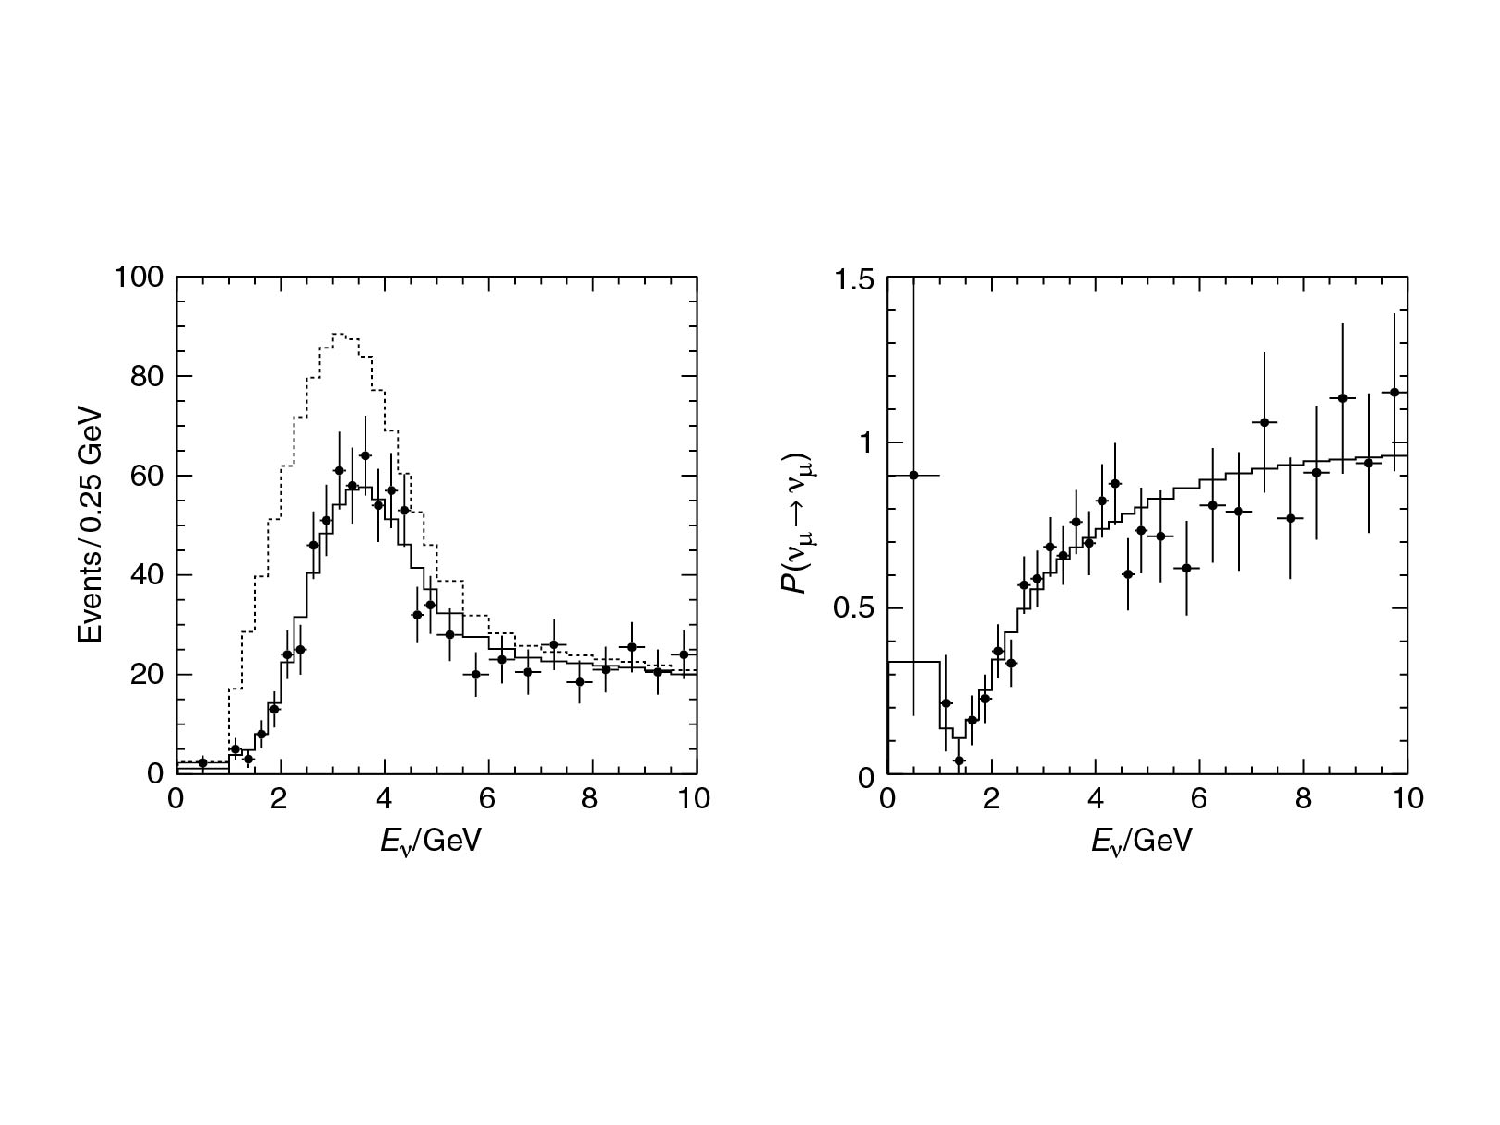
\includegraphics[width=0.90\textwidth,height=0.90\textheight,keepaspectratio]
                {pictures/t13_22.pdf}
  \vspace*{-20mm}
  \caption{Left: MINOS far detector energy spectrum and unoscillated
           prediction (dashed). Right: Muon neutrino survival probability
           as measured from the left figure. Image taken from Thomson
           Fig. 13.22 \cite{thomson_modern_2013}.}
  \label{fig:minos}
\end{figure}

We can calculate the muon neutrino survival probability for MINOS
using the same arguments as the beginning of this section. We can write
\begin{equation}
  \label{eq:sexyprob}
  \begin{aligned}
    \pr{\nu_\mu\to\nu_\mu}
      &\approx 1-4|U_{\mu1}|^2|U_{\mu2}|^2\sin^2\Delta_{21}
              -4|U_{\mu3}|^2\left(1-|U_{\mu3}|^2\right)\sin^2\Delta_{32} \\
      &\approx 1-\left(\sin^2(2\theta_{23})c_{13}^4
                       +\sin^2(2\theta_{13})s_{23}^2)\right)
                        \sin^2\Delta_{32},
  \end{aligned}
\end{equation}
where in the last step we have utilized the fact that the long wavelength
component can be ignored for MINOS. Fig. \ref{fig:minos} shows the 
results of the experiment. The left plot compares the observed far 
detector energy spectrum
with the unoscillated prediction, which gives a direct measurement of the
muon neutrino survival probability, shown on the right. According to 
\equatref{eq:sexyprob}, the minimum of the right plot yields
\cite{adamson_measurement_2011}
\begin{equation}
  |\Delta m_{32}^2|=(2.32^{+0.12}_{-0.08})\times10^{-3}~\text{eV}^2,
\end{equation}
and the best fit for $\theta_{23}$ yields the constraint
\begin{equation}
  \sin^2(2\theta_{23})\gtrsim0.90\
\end{equation}
at the 90\% confidence level.

\section{Conclusions, outlook}
As has been demonstrated, the experimental evidence supporting the existence of
neutrino oscillations is very strong. The three flavor oscillation model seems
to predict the data quite well, and from the above experiments, we've (more or
less) determined the values of the parameters of the PMNS matrix.
The success of the model has been a triumph for particle
physicists, but there is still more we need to learn. For example we don't yet
know whether the neutrino is a Majorana spinor, which could shed light on the
viability of the seesaw mechanism. We also have not yet found the
phase $\delta$ of the PMNS matrix. The SM could accommodate another light
neutrino species. And of course there is still room to pin down the exact
value for $\theta_{23}$. The sheer number of neutrino experiments currently
performed and in progress, along with the 2015 Nobel Prize, paints an
optimistic picture for the future of neutrino experiments.

\bibliographystyle{unsrtnat}
\bibliography{bibliography}

\chapter{Special Topic: The Higgs Boson}\label{ap:spec_higgs}

\index{Higgs!boson}
This appendix summarizes the importance of the Higgs boson in QFT and outlines
experiments leading up to the discovery of the Higgs boson.
First we discuss the issues of boson and fermion masses and explain
how the Higgs mechanism allows for such particles to exist in gauge invariant
theories. We apply this method to the standard model, and from this deduce
properties of the Higgs boson. The paper finally turns to preliminary results 
from LEP and Tevatron before concluding with the 2012 discovery at the LHC.

The Higgs mechanism is an example of SSB, so if you like, you can refresh
yourself by looking to \secref{sec:ssb}. In this chapter we will
also pay attention to the location of Lorentz indices again, as we
work with the physical Minkowski metric.

Since this chapter was adapted from a project I did as a grad student in 2014,
this chapter is likely not current.

\section{Gauge invariance in QFT}

Building a gauge-invariant Lagrangian is at the heart of constructing theories
of modern particle physics. There are a couple of reasons for demanding that a
theory not depend on gauge. For one, gauge-invariant theories have the nice
property of being renormalizable, a fact shown in 1972 by t'Hooft and Veltman 
\cite{t_hooft_regularization_1972}. Perhaps more importantly, utilizing gauge
invariance is an elegant way of deriving Lagrangians complete with terms
describing the observed interactions between gauge bosons and matter fields.

For example, consider a Lagrangian of the form
\begin{equation}
  \label{eq:genLagr}
  \Lagr=\bar{\psi}\slashed{D}\psi-\frac{1}{4}\tr F_{\mu\nu}F^{\mu\nu} ,
\end{equation}
where $D_{\mu}$ and $F_{\mu\nu}$ are respectively the gauge covariant
derivative and field strength
This is invariant under local gauge transformations. 
As mentioned previously, this is a desirable feature for the
Lagrangian to have, and hence it is a solid foundation off of which to build
a theory.

One notable feature about the Lagrangian~\eqref{eq:genLagr} is that
it does not allow for particles corresponding to gauge fields to have masses.
Consider for instance a naive mass term of the form $mA^{\mu}A_{\mu}$. Then 
under a local gauge transformation we would have
\begin{equation}
  \begin{aligned}
  mA'^{\mu}A'_{\mu}&=mUA_{\mu}U^{\dagger}UA^{\mu}U^{\dagger} \\
                   &=mUA_{\mu}A^{\mu}U^{\dagger},
  \end{aligned}
\end{equation}
which is in general not invariant. This suggests that the gauge bosons are
massless. While this is no contradiction for QED or QCD, this is in direct
opposition of observation that weak vector bosons have mass. Furthermore
electron mass terms of the form $\bar{\psi}_{L}\psi_{R}+
\bar{\psi}_{R}\psi_{L}$ are not invariant under 
$\SU(2)_{L}\times \U(1)_{Y}$ gauge transformations since left- and 
right-handed fermions
transform differently \cite{dittmaier_higgs_2013}.

\section{The Higgs mechanism}

\index{Higgs!mechanism}
Let us examine the mechanism responsible for reconciling the observation of 
massive gauge bosons with the desire for our theory to be gauge invariant. For 
the sake of simplicity, we consider a complex scalar field under a $\U(1)$ 
symmetry (scalar electrodynamics), but this procedure generalizes to 
non-abelian theories \cite{srednicki_quantum_2007}. 
We specify our Lagrangian by 
\begin{equation}
  \label{eq:HLagr1}
  \Lagr=-(D_{\mu}\phi)^{\dagger}D^{\mu}\phi-V(\phi)
              -\frac{1}{4}F_{\mu\nu}F^{\mu\nu},
\end{equation}
where $\phi$ is a complex scalar field, and
\begin{equation}
  \label{eq:pot}
  V(\phi)=m^{2}\phi^{\dagger}\phi+\frac{1}{4}\lambda(\phi^{\dagger}\phi)^{2}.
\end{equation}
We can identify the first term in \equatref{eq:pot} as representing the mass of
the particle and the second as representing self interactions of the field.
In the case $m^2>0$, the potential has a minimum at $|\phi|=0$, and we obtain 
the scalar electrodynamics to which we are accustomed. Now let us allow 
$m^2<0$. In this case, $V(\phi)$ takes its minimum on the circle defined by
\begin{equation}
  \label{eq:v2}
  \Re[\phi]^2+\Im[\phi]^2=v^2\equiv\frac{-4m^2}{\lambda}.
\end{equation}
The physical vacuum state will correspond to a point on this circle. (This
is the same case as depicted in \figref{fig:ssb}.) Choosing a state 
from among this continuum thus breaks the original
$\U(1)$ symmetry of the Lagrangian, which is an example of SSB. 

The vacuum expectation value (VEV) of the field is
\begin{equation}
  \bra{0}\phi(x)\ket{0}=\frac{v}{\sqrt{2}}.
\end{equation}
Let us find excited states by carrying out a perturbative expansion of $\phi$ 
about the vacuum state. We write
\begin{equation}
  \label{eq:phixpand}
  \begin{aligned}
  \phi(x)&=\frac{1}{\sqrt{2}}\big(v+h(x)+i\chi(x)\big) \\
         &\approx\frac{1}{\sqrt{2}}\big(v+h(x)\big)
                  e^{i\chi(x)/v}
  \end{aligned}
\end{equation}
to first order in the fields. (Here $h$ and $\chi$ are real.) Plugging 
\equatref{eq:phixpand} into \eqref{eq:pot}, using the definition of 
$v^2$, and throwing away the constant term (which of course does not change the 
physics) yields
\begin{equation}
  \label{eq:potnew}
  V(\phi)=\frac{1}{4}\lambda v^{2}h^{2}+\frac{1}{4}\lambda vh^{3}
          +\frac{1}{16}\lambda h^{4}.
\end{equation}
Since $V(\phi)$ is independent of $\chi$, the field must be massless,
and $\chi$ is the Goldstone boson for the broken symmetry. Since the
Lagrangian is gauge invariant, we can eliminate $\chi$ by making the
local transformation
\begin{equation}
  \phi(x)\to\phi'(x)=e^{-i\chi(x)/v}\phi(x).
\end{equation}
This choice of gauge is called the {\it unitary gauge}\index{unitary gauge}. 
In the unitary gauge
$\phi(x)$ becomes
\begin{equation}
  \label{eq:phinew}
  \phi(x)=\frac{1}{\sqrt{2}}\big(v+h(x)\big).
\end{equation}
We are finally in a position to physically interpret the fields. Plugging 
\equatref{eq:phinew} and \eqref{eq:potnew} into the first term of 
\eqref{eq:HLagr1} gives
\begin{equation}
  \label{eq:kin}
  \begin{aligned}
    -(D_{\mu})^{\dagger}(D^{\mu})&=-\frac{1}{2}(\partial_{\mu}h+ig(v+h)A_{\mu})
                                (\partial^{\mu}h-ig(v+h)A^{\mu}) \\
         &=-\frac{1}{2}\partial_{\mu}h\partial^{\mu}h 
           -\frac{1}{2}g^{2}(v^{2}+h^{2}+2vh)A_{\mu}A^{\mu}. 
  \end{aligned}
\end{equation} 
Viewed in this way, the gauge field has a mass
\begin{equation}
  M_{A}=gv.
\end{equation}
This process of eliminating the dependence of the Lagrangian on the Goldstone
boson combined while the gauge boson acquires a mass is called the {\it Higgs
mechanism}\index{Higgs!mechanism}. Furthermore the term quadratic in 
$h^2$ in \equatref{eq:potnew} shows the mass of the {\it Higgs field} 
$h$\index{Higgs!field} is
\begin{equation}
  M_{h}=\sqrt{2\lambda}v.
\end{equation}

Thus we see that out of our original Lagrangian falls a mass for the gauge
\index{Higgs!boson}
boson as well as for the {\it Higgs boson}, the boson corresponding to the
Higgs field. The Higgs mechanism has an admirable neatness to it. After all,
we found the boson by simply allowing $m^2<0$, which is perfectly justifiable
since we do not know {\it a priori} whether $\phi$ corresponds to a physical 
mass; in fact the Higgs mechanism suggests that rather than $\phi$, the
fields $h$ and $A^{\mu}$ are physical. Astonishingly, the Higgs mechanism
can also be used to fix the electron mass problem, which we will see in the
next section.

\section{The Standard Model Higgs}
The full Lagrangian of the Standard Model in its most general form is
\begin{equation}
  \label{eq:LSM}
  \Lagr_{\rm SM}=\Lagr_{\rm YM}+\Lagr_{\rm ferm}+\Lagr_{\rm Higgs}
                               +\Lagr_{\rm Yuk},
\end{equation}
where
\begin{equation}
  \label{eq:Ldefs}
  \begin{aligned}
    \Lagr_{\rm YM}&=-\frac{1}{4}W_{\mu\nu}^iW^{\mu\nu,i}
                -\frac{1}{4}B_{\mu\nu}B^{\mu\nu}
                -\frac{1}{4}G_{\mu\nu}^aG^{\mu\nu,a}, \\
    \Lagr_{\rm ferm}&= i\bar{\Psi}_{L}\slashed{D}\Psi_{L}
                  +i\bar{\psi}_{\ell_R}\slashed{D}\psi_{\ell_R}
                  +i\bar{\Psi}_{Q}\slashed{D}\Psi_{Q}
                  +i\bar{\psi}_{u_R}\slashed{D}\psi_{u_R}
                  +i\bar{\psi}_{d_R}\slashed{D}\psi_{d_R}, \\
    \Lagr_{\rm Higgs}&=(D_{\mu}\Phi)^{\dagger}(D^{\mu}\Phi)-V(\Phi), \\
    \Lagr_{\rm Yuk}&=-\bar{\Psi}_{L}G_{\ell}\psi_{\ell_R}\Phi
                 -\bar{\Psi}_{Q}G_{u}\psi_{u_R}\widetilde{\Phi}
                 -\bar{\Psi}_{Q}G_{d}\psi_{d_R}\Phi+h.c.,
  \end{aligned}
\end{equation}
$i$ runs from 1 to 3, and $a$ runs from 1 to 8. \cite{dittmaier_higgs_2013}. 
The interpretation 
of the first two terms is straightforward: The field strength 
tensors in the Yang-Mills part $\Lagr_{\rm YM}$ contain the 
kinetic terms of gauge 
fields as well as their self-interactions; $W$, $B$, and $G$ correspond to the 
weak, electromagnetic, and strong interactions, respectively. Meanwhile the 
fermion term $\Lagr_{\rm ferm}$ includes the couplings of gauge fields to the 
fermions, which are contained in
\begin{equation}
  D_{\mu}\equiv\partial_{\mu}+igI_{W}^{i}W_{\mu}^{i}
                  +ig'\frac{Y}{2}B_{\mu}+ig''T_{c}^{a}G_{\mu}^{a}.
\end{equation}
Here $I_{W}^{j}$, $Y_{W}$, and $T_c^{a}$ are the generators of the respective 
gauge groups, expressed in the same representation as the fermions on which 
they act.

To interpret the $\Lagr_{\rm Higgs}$, we employ the Higgs mechanism 
as before. The potential is
\begin{equation}
  \label{eq:Higgpot}
  V(\Phi)=m^2(\Phi^{\dagger}\Phi)+\frac{\lambda}{4}(\Phi^{\dagger}\Phi)^2
\end{equation}
and $\Phi$ is a complex scalar doublet
\begin{equation}
  \label{eq:newphi}
  \Phi=
  \begin{pmatrix}
    \phi^{+} \\
    \phi^{0}
  \end{pmatrix},
\end{equation}
where $\phi^{+}$ has charge $+e$ and $\phi^{0}$ has zero charge. We minimize
\equatref{eq:Higgpot} and spontaneously break the $\SU(2)_{L}\times\U(1)_{Y}$ 
symmetry while requiring the minimum correspond to a VEV only of $\phi^{0}$.
After expanding about the vacuum state in the unitary 
gauge (thereby eliminating any Goldstone bosons) we can write
\begin{equation}
  \label{eq:Higgsphi}
  \Phi=\frac{1}{\sqrt{2}}
  \begin{pmatrix}
    0 \\
    v+h
  \end{pmatrix}.
\end{equation}
To find the form of $\Lagr_{\rm Higgs}$ in this gauge, we plug in 
\equatref{eq:Higgsphi}
as well as the definitions of $W^{\pm}_{\mu}$ and the {\it weak mixing angle} 
$\theta_W$,
\begin{equation}
  W^{\pm}_{\mu}\equiv\frac{1}{\sqrt{2}}(W^{1}_{\mu}\mp iW^{2}_{\mu}),
  \ \ c_W\equiv\cos(\theta_W)\equiv\frac{gg'}{g^2+(g')^2},
\end{equation}
to obtain
\begin{equation}
  \label{eq:LagrHiggs}
  \begin{aligned}
    \Lagr_{\rm Higgs}&=\frac{1}{2}\partial_{\mu}h\partial^{\mu}h
                   +\frac{g^4}{4}(v+h)^{2}W^+_{\mu}W^{-\mu} \\
       & ~~~~~     +\frac{g^2}{8c_{W}^{2}}(v+h)^{2}Z_{\mu}Z^{\mu}
                   +\Big(\frac{\mu^2}{2}-\frac{\lambda}{16}\Big)(v+h)^{2} \\
       &=\frac{1}{2}\partial_{\mu}h\partial^{\mu}h
         -\frac{1}{2}M_{h}^{2}h^2 + M_{W}^{2}W^+_{\mu}W^{-\mu} \\
       & ~~~~~ +\frac{1}{2}M_{Z}^{2}Z_{\mu}Z^{\mu} 
         + gM_{W}hW^+_{\mu}W^{-\mu}
         +\frac{g^2}{4}h^{2}W^+_{\mu}W^{-\mu} \\
       & ~~~~~ +\frac{gM_{Z}}{2c_{W}}hZ_{\mu}Z^{\mu}
         +\frac{g^2}{4c_{W}^{2}}h^{2}Z_{\mu}Z^{\mu}
         -\frac{gM_{h}^2}{4M_W}h^3 - \frac{g^{2}M_{h}^2}{32M_{W}^2}h^4,
  \end{aligned}
\end{equation}
where we have neglected a constant term (as before) and used
\begin{equation}
  M_W\equiv\frac{gv}{2},\ \ M_Z\equiv\frac{M_W}{c_W},\ \
  M_h\equiv\sqrt{2m^2},\ \ v\equiv 2\sqrt{\frac{m^2}{\lambda}}.
\end{equation}
Hence we see that through SSB, the Higgs field has 
lent mass terms to the previously massless weak vector bosons, and that the 
photon has remained massless as desired. Perhaps more to the point of this 
section, we are able to glean important phenomenological predictions about the 
Higgs boson from the form of \equatref{eq:LagrHiggs}. Namely,
\begin{enumerate}
  \item the term quadratic in $h$ shows the Higgs has a mass $M_h$;
  \item the Higgs is spin-0 because the Higgs field is a scalar;
  \item it is neutral, since it is a perturbation of the vacuum state,
        which we required to be neutral when we broke the 
        $\SU(2)_{L}\times\U(1)_{Y}$ symmetry;
  \item it is CP even since, again, it is a vacuum excitation, and thus 
        carries the same quantum numbers as the vacuum;
  \item the three-vertex coupling of the Higgs to the $V=W,$ $Z$ bosons 
        is proportional to the mass of those bosons $M_V$, which we see from 
        $hV^{\dagger}V$ terms, while the four-vertex coupling is proportional
        to $M_{V}^2$, which comes from $h^{2}V^{\dagger}V$ terms (more
        precisely the coupling of the $hV^{\dagger}V$ term is $gM_{V}$, so we
        can also think of the coupling as being proportional to $M_{V}^{2}/v$,
        and similarly of the $h^{2}V^{\dagger}V$ coupling as proportional
        to $M_{V}^{2}/v^{2}$); 
        \vspace{9mm}
  \item the last two terms show cubic and quartic Higgs self-interactions;
  \item and the $W$ boson mass, $Z$ boson mass, and weak mixing angle are 
        related by $$\cos(\theta_W)=\frac{m_W}{m_Z}.$$
\end{enumerate}

Finally we consider the Yukawa part of the Standard Model Lagrangian. The
$h.c.$ in $\Lagr_{\rm Yuk}$ includes the hermitian conjugates of all the terms
preceding it. $\ell$, $u$, and $d$ refer to charged leptons, up-type quarks
(up, charm, top), and down-type quarks (down, strange, bottom), respectively.
$\widetilde{\Phi}$ is the Higgs doublet with opposite quantum numbers as
$\Phi$ and conjugated charge. The matrices $G_f$ mix left- and right-handed 
parts of different generations of the fermion type $f$ 
\cite{dittmaier_higgs_2013}. 

We can remove this mixing by transforming these matrices from the current 
{\it flavor basis} to the basis in which they are diagonal, the {\it mass 
basis}. In this basis
\begin{equation}
  G_f=\frac{\sqrt{2}}{v}\diag(m_{f_1},m_{f_2},m_{f_3}), 
\end{equation}
and $m_{f_i}$ can be interpreted as the mass of fermion $f_i$. Substituting
\equatref{eq:newphi} into $\Lagr_{\rm Yuk}$ and transforming to the 
unitary gauge, the Yukawa term becomes
\begin{equation}
  \Lagr_{\rm Yuk}=-\sum\limits_{f}m_{f}\Big(1+\frac{H}{v}\Big)
            (\bar{\psi}_{L_f}\psi_{R_f}+\bar{\psi}_{R_f}\psi_{L_f}),
\end{equation} 
where the sum is over all fermion flavors and all generations 
\cite{dittmaier_higgs_2013}. Cast
in this form, the Yukawa term gives us the prediction that
\begin{enumerate}
  \setcounter{enumi}{7}
  \item the Higgs boson couples to each fermion $f$ with strength $y_f=m_f/v$.
        This coupling constant is known as the {\it Yukawa coupling}.
\end{enumerate}
Hence we see that the issue of fermion masses has also been solved by the
Higgs mechanism. We note that in the lepton sector, the
change of basis is furnished by the same matrices for neutrinos as it is for
their corresponding charged particles only in the limit of massless neutrinos
\cite{dittmaier_higgs_2013}.


\section{How to find the Higgs}
Armed with our predictions from the previous section, we are in a favorable
position to motivate searches for the Higgs boson. We will see how searches for
the Higgs helped place a tight window on its expected mass, even though the 
mass is, in principle, a free parameter.
\begin{figure}
  \centering
  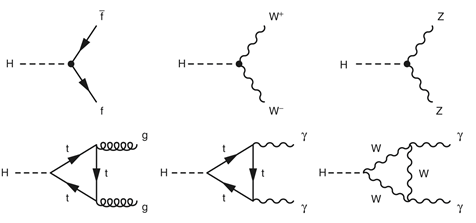
\includegraphics[width=0.75\textwidth,height=0.75\textheight,keepaspectratio]
                {pictures/higgs_decays.png}
  \caption{Example decay modes of the Higgs boson. Image taken from Thomson
           Figs. 17.14 and 17.16~\cite{thomson_modern_2013}.}
  \label{fig:exhiggsdecays}
\end{figure}

A preliminary step in accomplishing this goal is to decide which search 
channels to use. Knowing that the coupling of the Higgs boson to elementary 
bosons and fermions increases with the masses of those particles, one might be 
tempted to pick search channels whose Feynman diagrams involve the most massive
particles that are kinematically allowable. However there are 
also practical theoretical and experimental constraints that might make a 
channel with a smaller branching ratio a better candidate for search. The 
means to trigger signal events with high efficiency, suppress background 
radiation (e.g. multi-jet final states from other QCD interactions during a
hadron-hadron collision), and estimate uncertainties in signal and background 
predictions are also highly important, and were therefore taken into account by
scientists investigating the Higgs.

In addition to production channels, experimenters must decide which
decay modes to look for. Looking at the vertex factors above, the Higgs 
can decay into fermion-antifermion pairs as well as $W^{+}W^{-}$ and $ZZ$.
Furthermore the Higgs can decay into gluon-gluon and photon-photon pairs
through virtual quark and weak vector boson loops. For example Higgs decay
Feynman diagrams, see \figref{fig:exhiggsdecays},

As detailed in Dittmaier and Schumacher \cite{dittmaier_higgs_2013}, 
there were no tight
constraints on the Higgs mass prior to investigations at the Large Electron
Positron Collider (LEP). The primary search
channel there was $ZH$ production via ``Higgs-strahlung", for which the diagram
is shown in \figref{fig:higgsstrahlung}. 
The signal used at LEP was based on the $H\to b\bar{b}$ 
decay, which is not surprising since the bottom quark is the most 
massive fermion in the decay $H\to f\bar{f}$ for which $M_{h}>2M_{f}$. During
the LEP1 era (1989-1995), the collider operated at a CM energy of about $M_Z$. 
By the end of this era, the internal experiments ALEPH, DELPHI, L3, and OPAL 
together excluded Higgs boson masses below 63.2 GeV. Next the CM energy was
increased periodically from ~130 GeV in 1995 to 200 GeV in 2000--this is the
LEP2 era. By this time, the ability to identify b-flavored jets had been
greatly improved, which made it easier to distinguish signal and background. 
The final results of LEP2 showed a promising indication of the existence of
the Higgs, but were not strong enough to claim a discovery. Ultimately
the LEP2 experiments were able to exclude Higgs masses below 115 GeV with at
least 95\% confidence.

\begin{figure}
  \centering
  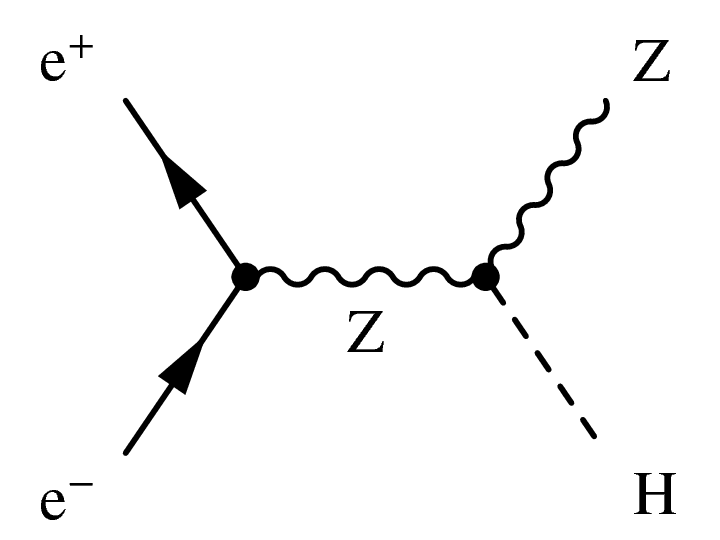
\includegraphics[width=0.40\textwidth,height=0.40\textheight,keepaspectratio]
                {pictures/higgsstrahlung.png}
  \caption{Leading order diagram for the production channel Higgs-strahlung. 
           Image taken from Simon \cite{simon_prospects_2013}.}
  \label{fig:higgsstrahlung}
\end{figure}

Besides electron-positron colliders, Higgs searches and exclusion experiments
have also taken place at hadron colliders, most notably the Tevatron at
Fermilab and the LHC at CERN. In 2001 the Tevatron Run II started with a CM 
energy of ~2 TeV. Running until 2011, the precision measurements at the
Tevatron suggested that the Higgs mass is less than 150 GeV, and not likely
larger than 200 GeV \cite{thomson_modern_2013}.

\section{Experimental evidence for the Higgs}
Between results from the LEP collider and Tevatron, high energy physicists
could have expected the Higgs mass to lie between 115 and 150 GeV. Nevertheless
the LHC and its two experiments ATLAS and CMS were designed to explore the
entire mass range from 115 GeV to ~1 TeV, which is the largest the Higgs mass
can be without violating unitarity \cite{dittmaier_higgs_2013}. The LHC is currently
the highest energy particle collider ever built and the highest luminosity 
proton-proton collider. Starting in 2010, the LHC operated at a CM energy of 7+
TeV, a drastic improvement over the energies of previous particle accelerators.
\begin{figure}
  \centering
  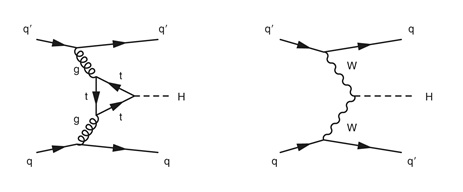
\includegraphics[width=0.75\textwidth,height=0.75\textheight,keepaspectratio]
                {pictures/higgs_prod_hadrons.png}
  \caption{Leading order diagrams for the Higgs boson production channels
           (left) gluon fusion and (right) vector boson fusion. Image taken 
           from Thomson Fig. 17.17~\cite{thomson_modern_2013}.}
  \label{fig:higgsfusion} 
\end{figure}

The primary search channels at the LHC were gluon fusion and vector boson
fusion, the Feynman diagrams of which are shown in \figref{fig:higgsfusion}. 
Because of the 
heavy masses of the top quarks, the gluon fusion process has a large cross 
section. However the gluon fusion process also leads to QCD radiation, which 
can make final states of this production channel difficult to distinguish from 
background QCD interactions. Meanwhile, the vector boson fusion final states 
consist only of Higgs boson decay products and forward jets from the colliding 
protons, making them more easily identifiable. Similarly the most
sensitive decay modes investigated were $H\to\gamma\gamma$, $H\to ZZ^{*}\to
\ell_{1}^{+}\ell_{1}^{-}\ell_{2}^{+}\ell_{2}^{-}$ (where $\ell_i$ is an 
electron or muon and the asterisk indicates that the $Z$-boson is off 
shell), and
$H\to WW^{*}\to e\nu_{e}\mu\nu_{\mu}$ because they can be more easily
distinguished from the background. The decays $H\to\gamma\gamma$ 
and $H\to ZZ^{*}\to4\ell$ also have the advantage that the mass of the Higgs 
can be more easily reconstructed from the masses of their decay products
\cite{dittmaier_higgs_2013}.

Although ATLAS and CMS searched the final states $\gamma\gamma$, $ZZ^{*}$,
$WW^{*}$, $\tau^{+}\tau^{-}$, and $b\bar{b}$, the most significant data came
from the $H\to \gamma\gamma$ and $H\to\ ZZ^{*}\to4\ell$ modes \cite{thomson_modern_2013}.
The reconstructed invariant mass distributions from ATLAS and CMS provided
statistically credible evidence for the existence of a new particle. Two
of the most significant distributions are shown in 
\figref{fig:higgsevidence}. In the ATLAS plot,
each event is weighted with the probability that it is kinematically compatible
with Higgs production and decay \cite{thomson_modern_2013}. We can see in both plots more events
than is expected from the background around a mass of 125 GeV, which we
identify as the Higgs. The peak at 91 GeV in the CMS plot can be attributed
to $Z$-boson production \cite{thomson_modern_2013}. 

Ultimately the discovered particle masses for each experiment were determined 
\cite{dittmaier_higgs_2013} to be
\begin{equation}
  \begin{aligned}
  M_{h({\rm ATLAS})}&=126.0\pm0.4(\text{stat})
                \pm0.4(\text{sys})\ \text{GeV}, \\
  M_{h({\rm CMS})}&=125.3\pm0.4(\text{stat})\pm0.5(\text{sys})\ \text{GeV}.
  \end{aligned}
\end{equation}
The fact that the new particle decays into a pair of particles with the same
spin and zero net charge shows that it is electrically neutral and has
integer spin. Hence by the spin statistics theorem, it is a neutral boson.
Furthermore by the Landau-Yang theorem, the fact that it can decay into two 
identical, massless, spin-1 particles shows that it cannot be a spin-1 particle
itself. Moreover the CMS Collaboration has recently been able to exclude many
spin-2 models for the Higgs at a confidence level of 99\% or higher 
\cite{khachatryan_constraints_2015}.
These observations together suggest that the particle found at the LHC is 
almost certainly the Higgs boson.

\begin{figure}
  \centering
  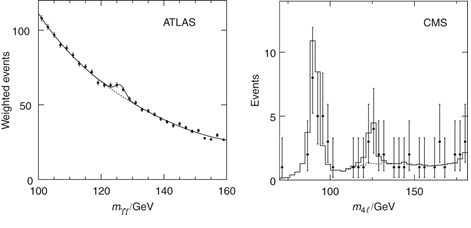
\includegraphics[width=0.75\textwidth,height=0.75\textheight,keepaspectratio]
                {pictures/higgs_results.png}
  \caption{Reconstructed invariant mass distribution plots. Solid lines
           indicate signal plus background expectation while dashed lines
           indicate background only expectation. The left corresponds to 
           $h\to\gamma\gamma$ decays measured at ATLAS while the right shows
           $h\to ZZ^{*}\to4\ell$ decays measured at CMS. Image taken from 
           Thomson Fig. 17.19~\cite{thomson_modern_2013}.}
  \label{fig:higgsevidence}
\end{figure}

\section{Future searches and conclusion}
There is still much about the
Higgs we must investigate and properties we must verify. We do not know, for
instance, if it is even under CP or whether it is spin-0. We 
haven't yet demonstrated that the Higgs couples to itself. The choice of one 
Higgs doublet is the most conservative, but it is possible to use more; in 
particular supersymmetric theories utilize at least two Higgs doublets 
\cite{thomson_modern_2013}. Finally, it is possible that the 
Higgs is a composite particle. 

\bibliographystyle{unsrtnat}
\bibliography{bibliography}
                               


\chapter{Special Topic: The Standard Model}\label{ap:spec_SM}

For this appendix we will roughly write the Lagrangian for the Standard Model in the
$R_\xi$ gauge and write down some of the corresponding Feynman rules. We will
make some general considerations involving two particle decays. Next we
specialize to the Feynman gauge and calculate decay rates for some of
the most important decay channels of the Higgs. 
%Finally we will compare our
%results to some known values to see how we did.

\section{The SM Lagrangian}
This section is based heavily off of Bardin and 
Passarino~\cite{bardin_standard_1999}. Unlike
them, however, we will use the metric with signature $(+\ -\ -\ -)$ and we will
\index{gauge!fixing}
define the gauge-fixing term slightly differently when we come to it.
Ultimately our Feynman rules should agree with Peskin and 
Schroeder~\cite{peskin_introduction_1995}.

We begin with the electroweak sector. The fields include a triplet of vector
bosons $B_{\mu}^{a}$ and a vector singlet $B_{\mu}^{0}$; a complex scalar
\index{Faddeev-Popov ghost}
doublet $K$; Faddeev-Popov (FP) ghost fields $X^{\pm}$, $Y^Z$, $Y^A$; and
fermions. The physical fields $Z$ and $A$ are given by
\begin{equation}
  \left(\begin{array}{c}
    Z \\
    A
  \end{array}\right)
  =
  \left(\begin{array}{cc}
    \ct & -\st \\
    \st & \ct
  \end{array}\right)
  \left(\begin{array}{c}
    B^3 \\
    B^0
  \end{array}\right),
\end{equation}
where $\st\coloneqq\sin\big(\theta_{W}\big)$,
$\ct\coloneqq\cos\big(\theta_{W}\big)$, and $\theta_W$ is the weak
mixing angle. The scalar field for the minimal Higgs model is
\begin{equation}
  \label{eq:Hsf}
  K=\frac{1}{\sqrt{2}}
  \left(\begin{array}{c}
    H+2M_{W}/g+i\phi^0 \\
    \sqrt{2}i\phi^-
  \end{array}\right),
\end{equation}
where $H$ is the physical Higgs field, $M_W$ is the bare $W$-boson mass, and
$g$ is the bare $SU(2)$ coupling. The first part of the Lagrangian is
\begin{equation}
  \Lagr_{gauge}=\Lagr_{YM}+\Lagr_{H},
\end{equation}
where
% what is \epsilon?
\begin{equation}
  \begin{aligned}
    \Lagr_{YM}&=-\frac{1}{4}F_{\mu\nu}^{a}F^{\mu\nu,a}
                -\frac{1}{4}F_{\mu\nu}^{0}F^{\mu\nu,0} \\
    \Lagr_{H}&=-\big(D_{\mu}K\big)^{\dagger}\big(D^{\mu}K\big)
               -\mu^2 K^{\dagger}K 
               -\frac{\lambda}{2}\big(K^{\dagger}K\big)^2 \\
    F_{\mu\nu}^{a}&=\partial_{\mu}B_{\nu}^{a}-\partial_{\nu}B_{\mu}^{a}
                   +g\epsilon^{abc}B_{\mu}^{b}B_{\nu}^{c} \\
    F_{\mu\nu}^{0}&=\partial_{\mu}B_{\nu}^{0}-\partial_{\nu}B_{\mu}^{0}
  \end{aligned}
\end{equation}
and we need $\lambda>0$ (to have a ground state) and $\mu^2<0$ (for spontaneous
symmetry breaking). The $SU(2)\times U(1)$ gauge covariant derivative is
\begin{equation}
  \label{eq:SU2U1cd}
  D_{\mu}=\partial_{\mu}-\frac{i}{2}gB_{\mu}^{a}\sigma^{a}
                       -\frac{i}{2}gg'B_{\mu}^{0},
\end{equation}
where $\sigma^{a}$ are the Pauli matrices, and $g'=-\st/\ct$.
Also \eqref{eq:Hsf} can be rewritten as
\begin{equation}
  \label{eq:Hsf2}
  K=\frac{1}{\sqrt{2}}\Big(H+\frac{2M_W}{g}+i\phi^{a}\sigma^{a}\Big)
  \left(\begin{array}{c}
    1 \\
    0
  \end{array}\right).
\end{equation}

Next let us write
\begin{equation}
  \Lagr_{gauge}=\Lagr_{YM}-\big(D_{\mu}K\big)^{\dagger}\big(D^{\mu}K\big)
                 +\Lagr_{int}.
\end{equation}
If we were to calculate $\big(D_{\mu}K\big)^{\dagger}\big(D^{\mu}K\big)$ using
\eqref{eq:SU2U1cd} and \eqref{eq:Hsf2}, collect terms proportional to $v^2$,
where
\begin{equation}
  v=\frac{2M_W}{g},
\end{equation}
and use the field definitions
\begin{equation}
  W_{\mu}^{\pm}\coloneqq\frac{1}{\sqrt{2}}\big(B_{\mu}^1 \mp iB_{\mu}^2\big)
  \qquad
  \phi^{\pm}\coloneqq\frac{1}{\sqrt{2}}\big(\phi^1 \mp i\phi^2 \big),
\end{equation}
we would get
\begin{equation}
  \begin{aligned}
    \big(D_{\mu}K\big)^{\dagger}\big(D^{\mu}K\big)&=-\frac{g^2 v^2}{8}
      \Bigg(\frac{1}{\ct^2}Z_{\mu}Z^{\mu}+2W^+_{\mu}W^{-\mu}\Bigg)+...\\
    &=-\frac{1}{2}M_Z^2 Z_{\mu}Z^{\mu}-M_W^2 W_{\mu}^+ W^{-\mu}+...
  \end{aligned}
\end{equation}
where
\begin{equation}
  M_Z \coloneqq\frac{gv}{2\ct}=\frac{M_W}{\ct}.
\end{equation}
Hence we see that through the Higgs mechanism the $W$- and $Z$-bosons
acquired mass.
Now let us focus on terms of $(D_{\mu}K\big)^{\dagger}\big(D^{\mu}K\big)$ that
do not have any power of $g$ (besides kinetic terms). We get
\begin{equation}
  \label{eq:zmp}
  \big(D_{\mu}K\big)^{\dagger}\big(D^{\mu}K\big)=-M_W \Bigg(
     \frac{1}{\ct}Z_{\mu}\partial^{\mu}\phi^0 +W_{\mu}^+ \partial^{\mu}\phi^-
     +W_{\mu}^- \partial^{\mu}\phi^+ \Bigg).
\end{equation}
This part of the Lagrangian contains $Z$-$\phi^0$ and
$W^{\pm}$-$\phi^{\pm}$ interactions, and although they are zeroth order
in the field, they must be summed over when we develop perturbation theory.
Here the Lagrangian is badly divergent.

To fix this problem, we follow the usual prescription of introducing a 
gauge-fixing term, then introducing FP ghost fields to maintain gauge invariance. We
\index{gauge!fixing}
work in the generalized $R_{\xi}$ gauge. (The Feynman gauge corresponds to
$\xi=1$, the Lorenz to $\xi=0$, and the unitary to $\xi\to\infty$.) In this
gauge, the gauge-fixing piece is
\begin{equation}
  \Lagr_{gf}=-\frac{1}{2}C^a C^a -\frac{1}{2}\big(C^0\big)^2
            =-C^+ C^- -\frac{1}{2}\Big(\big(C^3\big)^2\big(C^0\big)^2\Big),
\end{equation}
where the gauge-fixing function is
\begin{equation}
  C^a =\frac{1}{\sqrt{\xi}}\big(\partial_{\mu}B^{a\mu}
                -\xi M_W \phi^a \big)
\end{equation}
and
\begin{equation}
  \label{eq:cdefs}
  C^{\pm}=\frac{1}{\sqrt{\xi}}\big(\partial_{\mu}W^{\pm\mu}
                   -\xi M_W \phi^{\pm}\big) \qquad
  C^{0}=\frac{1}{\sqrt{\xi}}\big(\partial_{\mu}B^{0\mu}
                   -\xi\frac{\st}{\ct}M_W \phi^{0}\big).
\end{equation}
Then we write
\begin{equation}
  -\frac{1}{2}\Big(\big(C^3\big)^2 +\big(C^0\big)^2\Big)
       =-\frac{1}{2}C_Z^2 -\frac{1}{2}C_A^2
\end{equation}
so that in the so-called $Z$-$A$ basis
\begin{equation}
  \label{eq:zadefs}
  C_A=\frac{1}{\sqrt{\xi}}\partial_{\mu}A^{\mu} \qquad
  C_Z=\frac{1}{\sqrt{\xi}}\partial_{\mu}Z^{\mu}-\xi\frac{M_W}{\ct}\phi^0.
\end{equation}
The Lagrangian including gauge-fixing terms is thus
\begin{equation}
  \Lagr_{YM}=-\big(D_{\mu}K\big)^{\dagger}\big(D^{\mu}K\big)-C^+ C^-
               -\frac{1}{2}C_Z^2-\frac{1}{2}C_Z^2
            =\Lagr_{prop}+\Lagr_{int}^{bos}
\end{equation}
and contains no divergent terms such as those in \eqref{eq:zmp}. $\Lagr_{prop}$
contains the terms that give rise to gauge EW propagators as well as mass
terms. Let us examine some terms relevant to Higgs processes. We have
\begin{equation}
  \begin{aligned}
  \Lagr_{prop}=&-\partial_{\mu}W_{\nu}^+ \partial^{\mu}W^{-\nu}
     +\Bigg(1-\frac{1}{\xi}\Bigg)\partial_{\mu}W^{+\mu}\partial_{\nu}W^{-\nu}
     -M_W^2 W_{\mu}^+ W^{-\mu} \\
    &-\frac{1}{2}\partial_{\mu}Z_{\nu}\partial^{\mu}Z^{\nu}
     +\frac{1}{2}\Bigg(1-\frac{1}{\xi}\Bigg)\big(\partial_{\mu}Z^{\mu}\big)^2
     -\frac{1}{2}M_Z^2 Z_{\mu}Z^{\mu} \\
    &-\partial_{\mu}\phi^+ \partial^{\mu}\phi^- -\xi M_W^2\phi^+ \phi^-
     +...
  \end{aligned}
\end{equation}
First of all we see that the Goldstone boson mass is proportional $\sqrt{\xi}$,
which means it's unphysical. (We would find the same for $\phi^0$.) Furthermore
the first line, second line, and third line yield respectively the Feynman
rules
\begin{equation*}
  \frac{-ig^{\mu\nu}}{k^2-M_W^2+i\epsilon}~~\F1~~~~~~~~
  \frac{-ig^{\mu\nu}}{k^2-M_Z^2+i\epsilon}~~\F2~~~~~~~~
  \frac{i}{p^2-\xi M_W^2+i\epsilon}~~\F3
\end{equation*}
\begin{figure}
  \centering
  \begin{fmffile}{fr123}
    \begin{subfigure}{0.3\textwidth}
      \centering
      \begin{fmfgraph*}(70,60)
        \fmfleft{i}
        \fmfright{o}
        \fmflabel{$\mu$}{i}
        \fmflabel{$\nu$}{o}
        \fmf{photon,label=$W^\pm$}{i,o}
      \end{fmfgraph*}
    \caption*{\F1}
    \end{subfigure}
    \begin{subfigure}{0.3\textwidth}
      \centering
      \begin{fmfgraph*}(70,60)
        \fmfleft{i}
        \fmfright{o}
        \fmflabel{$\mu$}{i}
        \fmflabel{$\nu$}{o}
        \fmf{photon,label=$Z$}{i,o}
      \end{fmfgraph*}
    \caption*{\F2}
    \end{subfigure}
    \begin{subfigure}{0.3\textwidth}
      \centering
      \begin{fmfgraph*}(70,60)
        \fmfleft{i}
        \fmfright{o}
        \fmf{dashes,label=$\phi^\pm$}{i,o}
      \end{fmfgraph*}
    \caption*{\F3}
    \end{subfigure}
  \end{fmffile}
  \caption{Electroweak gauge boson propagators (except photon) and Goldstone
           boson propagator.}
\end{figure}

Meanwhile $\Lagr_{int}^{bos}$ contains the interaction terms of the vector
bosons with each other and the Higgs. We will focus on the terms
\begin{equation}
  \begin{aligned}
    \Lagr_{int}^{bos}=&-ig\ct\Big\{\partial_\nu Z_\mu W^{[+\mu}W^{-\nu ]}
                       -Z_\nu W_\mu^{[+}\partial^\nu W^{-\mu ]}
                       +Z_\mu W_\nu^{[+}\partial^\nu W^{-\mu ]}\Big\}\\
                      &-ie\Big\{\partial_\nu A_\mu W^{[+\mu}W^{-\nu]}
                       -A_\nu W_\mu^{[+}\partial^\nu W^{-\mu ]}
                       +A_\mu W_\nu^{[+}\partial^\nu W^{-\mu ]}\Big\}\\
                      &+e^2 \Big\{A_\mu A_\nu W^{+\mu}W^{-\nu}
                       +A_\mu A^\mu W^+_\nu W^{-\nu}\Big\}\\
                      &+eg\ct\Big\{A_\mu Z_\nu W^{[+\mu}W^{-\nu ]}
                       -2A_\mu Z^\mu W^+_\nu W^{-\nu}\Big\}\\
                      &+ig\frac{\ct^2-\st^2}{\ct}Z_\mu
                         \Big\{\phi^+ \partial^\mu \phi^-
                               -\phi^- \partial^\mu \phi^+ \Big\}\\
                      &+\frac{1}{2}g
                         \Big\{W_\mu^+\big(H\partial^\mu\phi^- 
                               -\phi^-\partial^\mu H\big)
                              -W_\mu^-\big(H\partial^\mu\phi^+ 
                               -\phi^+\partial^\mu H\big)\Big\}\\
                      &+ieM_W A_\mu W^{[+\mu}\phi^{-]}
                       -igM_Z \st^2 Z_\mu W^{[+\mu}\phi^{-]}
                       -gM_W H W_\mu^+ W_\nu^- \\
                      &-e^2 A_\mu A^\mu \phi^+ \phi^-
                       +\frac{i}{2}egA_\mu HW^{[+\mu}\phi^{-]}
                       -eg\frac{\ct^2-\st^2}{\ct}Z_\mu A^\mu \phi^+ \phi^- \\
                      &+ieA_\mu \big(\phi^+\partial^\mu\phi^-
                                     -\phi^-\partial^\mu\phi^+\big)
                       +...
  \end{aligned}
\end{equation}
where $e=g\st$ and $A^{[+}B^{-]}=A^+ B^- -B^- A^+$. The corresponding Feynman
rules are
\begin{gather*}
  ig\ct\big(g^{\alpha\beta}(p-k)^\mu+g^{\beta\mu}(k-q)^\mu
            +g^{\mu\alpha}(q-p)^\beta\big)~~\F4 \\
  -ie\big(g^{\alpha\beta}(p-k)^\mu+g^{\beta\mu}(k-q)^\mu
          +g^{\mu\alpha}(q-p)^\beta\big)~~\F5 \\
  -ie^2\big(2g^{\alpha\beta}g^{\mu\nu}-g^{\alpha\mu}g^{\beta\nu}
            -g^{\alpha\nu}g^{\beta\mu}\big)~~\F6 \\
  ieg\ct\big(2g^{\alpha\beta}g^{\mu\nu}-g^{\alpha\mu}g^{\beta\nu}
            -g^{\alpha\nu}g^{\beta\mu}\big)~~\F7 \\
  ig\frac{\cos(2\theta_W)}{2\ct}(p_+-p_-)^\mu~~\F8~~~~~~~~
  \mp\frac{ig}{2}(k-p)^\mu~~\F9~~~~~~~~
  -ieM_Wg^{\mu\nu}~~\F{10} \\
  -igM_Z \st^2 g^{\mu\nu}~~\F{11}~~~~~~~~
  igM_Wg^{\mu\nu}~~\F{12}~~~~~~~~
  2ie^2g^{\mu\nu}~~\F{13} \\
  -\frac{i}{2}egg^{\mu\nu}~~\F{14}~~~~~~~~
  -ieg\frac{\cos(2\theta_W)}{\ct}g^{\mu\nu}~~\F{15}~~~~~~~~
  -ie(p_+-p_-)^\mu~~\F{16}
\end{gather*}
\begin{figure}
  \centering
  \begin{fmffile}{fr4to17}
    \begin{subfigure}{0.3\textwidth}
      \centering
      \begin{fmfgraph*}(60,60)
        \fmfleft{i1,i2}
        \fmfright{o}
        \fmf{photon,label=$k$}{i1,v}
        \fmf{photon,label=$p$}{i2,v}
        \fmf{photon,label=$q$}{v,o}
        \fmflabel{$W_\beta^+$}{i1}
        \fmflabel{$W_\alpha^-$}{i2}
        \fmflabel{$Z_\mu$}{o}
      \end{fmfgraph*}
    \caption*{\F4}
    \end{subfigure}
    \begin{subfigure}{0.3\textwidth}
      \centering
      \begin{fmfgraph*}(60,60)
        \fmfleft{i1,i2}
        \fmfright{o}
        \fmf{photon,label=$k$}{i1,v}
        \fmf{photon,label=$p$}{i2,v}
        \fmf{photon,label=$q$}{v,o}
        \fmflabel{$W_\beta^+$}{i1}
        \fmflabel{$W_\alpha^-$}{i2}
        \fmflabel{$A_\mu$}{o}
      \end{fmfgraph*}
    \caption*{\F5}
    \end{subfigure}
    \begin{subfigure}{0.3\textwidth}
      \centering
      \begin{fmfgraph*}(60,60)
        \fmfleft{i1,i2}
        \fmfright{o1,o2}
        \fmf{photon}{i1,v}
        \fmf{photon}{i2,v}
        \fmf{photon}{v,o1}
        \fmf{photon}{v,o2}
        \fmflabel{$W_\alpha^+$}{i2}
        \fmflabel{$A_\mu$}{i1}
        \fmflabel{$W_\beta^-$}{o2}
        \fmflabel{$A_\nu$}{o1}
      \end{fmfgraph*}
    \caption*{\F6}
    \end{subfigure} \\
    \vspace{12mm}
   \begin{subfigure}{0.3\textwidth}
      \centering
      \begin{fmfgraph*}(60,60)
        \fmfleft{i1,i2}
        \fmfright{o1,o2}
        \fmf{photon}{i1,v}
        \fmf{photon}{i2,v}
        \fmf{photon}{v,o1}
        \fmf{photon}{v,o2}
        \fmflabel{$W_\alpha^+$}{i2}
        \fmflabel{$A_\mu$}{i1}
        \fmflabel{$W_\beta^-$}{o2}
        \fmflabel{$Z_\nu$}{o1}
      \end{fmfgraph*}
    \caption*{\F7}
    \end{subfigure}
    \begin{subfigure}{0.3\textwidth}
      \centering
      \begin{fmfgraph*}(60,60)
        \fmfleft{i1,i2}
        \fmfright{o}
        \fmf{dashes,label=$p_-$}{i1,v}
        \fmf{dashes,label=$p_+$}{i2,v}
        \fmf{photon}{v,o}
        \fmflabel{$\phi^-$}{i1}
        \fmflabel{$\phi^+$}{i2}
        \fmflabel{$Z_\mu$}{o}
      \end{fmfgraph*}
    \caption*{\F8}
    \end{subfigure}
    \begin{subfigure}{0.3\textwidth}
      \centering
      \begin{fmfgraph*}(60,60)
        \fmfleft{i1,i2}
        \fmfright{o}
        \fmf{dashes,label=$p$}{i1,v}
        \fmf{dashes,label=$k$}{i2,v}
        \fmf{photon}{v,o}
        \fmflabel{$\phi^\mp$}{i1}
        \fmflabel{$H$}{i2}
        \fmflabel{$W^\pm_\mu$}{o}
      \end{fmfgraph*}
    \caption*{\F9}
    \end{subfigure} \\
    \vspace{12mm}
    \begin{subfigure}{0.3\textwidth}
      \centering
      \begin{fmfgraph*}(60,60)
        \fmfleft{i1,i2}
        \fmfright{o}
        \fmf{photon}{i1,v}
        \fmf{dashes}{i2,v}
        \fmf{photon}{v,o}
        \fmflabel{$W_\nu^\pm$}{i1}
        \fmflabel{$\phi^\mp$}{i2}
        \fmflabel{$A_\mu$}{o}
      \end{fmfgraph*}
    \caption*{\F{10}}
    \end{subfigure}
    \begin{subfigure}{0.3\textwidth}
      \centering
      \begin{fmfgraph*}(60,60)
        \fmfleft{i1,i2}
        \fmfright{o}
        \fmf{photon}{i1,v}
        \fmf{dashes}{i2,v}
        \fmf{photon}{v,o}
        \fmflabel{$W_\nu^\pm$}{i1}
        \fmflabel{$\phi^\mp$}{i2}
        \fmflabel{$Z_\mu$}{o}
      \end{fmfgraph*}
    \caption*{\F{11}}
    \end{subfigure}
    \begin{subfigure}{0.3\textwidth}
      \centering
      \begin{fmfgraph*}(60,60)
        \fmfleft{i1,i2}
        \fmfright{o}
        \fmf{photon}{i1,v}
        \fmf{dashes}{i2,v}
        \fmf{photon}{v,o}
        \fmflabel{$W_\nu^\mp$}{i1}
        \fmflabel{$H$}{i2}
        \fmflabel{$W_\mu^\pm$}{o}
      \end{fmfgraph*}
    \caption*{\F{12}}
    \end{subfigure} \\
    \vspace{12mm}
    \begin{subfigure}{0.3\textwidth}
      \centering
      \begin{fmfgraph*}(60,60)
        \fmfleft{i1,i2}
        \fmfright{o1,o2}
        \fmf{dashes}{i1,v}
        \fmf{dashes}{i2,v}
        \fmf{photon}{v,o1}
        \fmf{photon}{v,o2}
        \fmflabel{$\phi^+$}{i2}
        \fmflabel{$\phi^-$}{i1}
        \fmflabel{$A_\mu$}{o2}
        \fmflabel{$A_\nu$}{o1}
      \end{fmfgraph*}
    \caption*{\F{13}}
    \end{subfigure}
    \begin{subfigure}{0.3\textwidth}
      \centering
      \begin{fmfgraph*}(60,60)
        \fmfleft{i1,i2}
        \fmfright{o1,o2}
        \fmf{dashes}{i1,v}
        \fmf{dashes}{i2,v}
        \fmf{photon}{v,o1}
        \fmf{photon}{v,o2}
        \fmflabel{$\phi^\pm$}{i2}
        \fmflabel{$H$}{i1}
        \fmflabel{$W_\mu^\mp$}{o2}
        \fmflabel{$A_\nu$}{o1}
      \end{fmfgraph*}
    \caption*{\F{14}}
    \end{subfigure}
    \begin{subfigure}{0.3\textwidth}
      \centering
      \begin{fmfgraph*}(60,60)
        \fmfleft{i1,i2}
        \fmfright{o1,o2}
        \fmf{dashes}{i1,v}
        \fmf{dashes}{i2,v}
        \fmf{photon}{v,o1}
        \fmf{photon}{v,o2}
        \fmflabel{$\phi^+$}{i2}
        \fmflabel{$\phi^-$}{i1}
        \fmflabel{$Z_\mu$}{o2}
        \fmflabel{$A_\nu$}{o1}
      \end{fmfgraph*}
    \caption*{\F{15}}
    \end{subfigure} \\
    \vspace{12mm}
   \begin{subfigure}{0.3\textwidth}
      \centering
      \begin{fmfgraph*}(60,60)
        \fmfleft{i1,i2}
        \fmfright{o}
        \fmf{dashes,label=$p_-$}{i1,v}
        \fmf{dashes,label=$p_+$}{i2,v}
        \fmf{photon}{v,o}
        \fmflabel{$\phi^-$}{i1}
        \fmflabel{$\phi^+$}{i2}
        \fmflabel{$A_\mu$}{o}
      \end{fmfgraph*}
    \caption*{\F{16}}
    \end{subfigure}
    \begin{subfigure}{0.3\textwidth}
      \centering
      \begin{fmfgraph*}(60,60)
        \fmfleft{i1,i2}
        \fmfright{o}
        \fmf{dashes,label=$p_-$}{i1,v}
        \fmf{dashes,label=$p_+$}{i2,v}
        \fmf{dashes}{v,o}
        \fmflabel{$\phi^-$}{i1}
        \fmflabel{$\phi^+$}{i2}
        \fmflabel{$H$}{o}
      \end{fmfgraph*}
    \caption*{\F{17}}
    \end{subfigure}
  \end{fmffile}
  \caption{Some interaction diagrams between electroweak bosons, Goldstone
           bosons, and the Higgs. Momentum arrows are taken to be toward
           the vertex center.}
\end{figure}

The interactions among only Higgs and Goldstone fields emerge from the Higgs
potential
\begin{equation}
  \Lagr_{int}^H=-\mu^2 K^\dagger K-\frac{\lambda}{2}\big(K^\dagger K\big)^2
\end{equation}
after spontaneous symmetry breaking. The only one from this sector that we
will need is
\begin{equation}
  \Lagr_{int}^H=\frac{1}{2}g\frac{M_H^2}{M_W}H\phi^+ \phi^- +...
\end{equation}
and the corresponding Feynman rule is
\begin{gather*}
  -\frac{ig}{2}\frac{M_H^2}{M_W}~~\F{17}
\end{gather*}


To finish off the scalar part of the electroweak sector, we introduce the FP
Lagrangian, which we accomplish by taking gauge transformations of the $C^a$.
The gauge transformations of the bosonic fields are
\begin{gather}
  B_\mu^a\to B_\mu^a+g\epsilon^{abc}\Lambda^bB^c_\mu \qquad
  B^0_\mu\to B^0_\mu-\partial_\mu\Lambda^0 \\
  K\to \Bigg(1-\frac{ig}{2}\Lambda^2\sigma^a-\frac{i}{2}gg'\Lambda^0\Bigg)K
\end{gather}
The $\Lambda^i,i=0,1,2,3$ are the group gauge transformation parameters. The
physical gauge transformation parameters $\Lambda^j,j=+,-,Z,A$ are
specified by
\begin{gather}
  \label{eq:lparam}
  \Lambda^1=\frac{1}{\sqrt{2}}\big(\Lambda^++\Lambda^-\big) \qquad
  \Lambda^2=\frac{i}{\sqrt{2}}\big(\Lambda^+-\Lambda^-\big) \\
  \nonumber
  \Lambda^3=\ct\Lambda^Z+\st\Lambda^A \qquad
  \Lambda^0=-\st\Lambda^Z+\ct\Lambda^A \\
  \nonumber
  \Lambda^3+g'\Lambda^0=\frac{1}{\ct}\Lambda^Z \qquad
  -\Lambda^3+g'\Lambda^0=-\frac{\ct^2-\st^2}{\ct}\Lambda^Z-2\st\Lambda^A.
\end{gather}
Using \eqref{eq:lparam} we can derive the gauge transformations of the
physical fields in terms of the physical parameters. Combining this with
\eqref{eq:cdefs} and \eqref{eq:zadefs}, we get the gauge transformations of
$C^\pm,C^A,$ and $C^Z$ in terms of physical parameters. For the purposes
of this exam, the most important part is
\begin{equation}
  \label{eq:cxform}
  C^\pm \to C^\pm +\frac{1}{\sqrt{\xi}}\big(\Box\Lambda^\pm
                         +\xi M_W^2 \Lambda^\pm\big)+...
\end{equation}
where $\Box$ is the D'Alembertian operator. Just as in the case of gauge
fields, we associate with each physical gauge parameter
$\Lambda^\pm,\Lambda^Z,\Lambda^A$ a ghost field $X^\pm,Y^Z,Y^A$ by
\begin{gather}
  X^1=\frac{1}{\sqrt{2}}\big(X^++X^-\big), \qquad
  X^2=\frac{1}{\sqrt{2}}\big(X^+-X^-\big), \\
  X^3=\ct Y^Z+\st Y^A, \qquad
  X^0=-\st Y^Z +\ct Y^A. \nonumber
\end{gather}
The gauge
invariance $C^\pm\to C^\pm$ is restored if we identify the first term in
\eqref{eq:cxform} as the ghost propagator
\begin{gather*}
  \frac{i}{k^2-\xi M_W^2+i\epsilon}~~\F{18}
\end{gather*}
and identify ghost field interactions of the form
\begin{equation}
  g\overline{X}^i L^{ij} X^j, \qquad i,j=+,-,Z,A.
\end{equation}
The interaction Lagrangian for the electroweak ghosts then becomes (again
we're only looking at some of the terms)
\begin{gather}
  \Lagr_{int}^{gf}=ie\frac{1}{\sqrt{\xi}}A_\mu
                       \big(\partial^\mu \overline{X}^+X^+
                            -\partial^\mu \overline{X}^-X^-\big)
                   +ig\ct\frac{1}{\sqrt{\xi}}Z_\mu
                       \big(\partial^\mu \overline{X}^+X^+
                            -\partial^\mu \overline{X}^-X^-\big)\\
                   -\frac{1}{2}g\sqrt{\xi}M_W H
                   \big(\overline{X}^+X^+ -\overline{X}^-X^-\big)+...\nonumber
\end{gather}
with Feynman rules
\begin{gather*}
 \mp iep^\mu~~\F{19}~~~~~~~~
 \pm ig\ct p^\mu~~\F{20}~~~~~~~~
 -\frac{ig}{2}\sqrt{\xi}M_W~~\F{21}
\end{gather*}
\begin{figure}
  \begin{fmffile}{fr18to21}
  \centering
    \begin{subfigure}{0.45\textwidth}
      \centering
      \begin{fmfgraph*}(60,60)
        \fmfleft{i}
        \fmfright{o}
        \fmf{dots,label=$X^\pm$}{i,o}
      \end{fmfgraph*}
    \caption*{\F{18}}
    \end{subfigure}
    \begin{subfigure}{0.45\textwidth}
      \centering
      \begin{fmfgraph*}(60,60)
        \fmfleft{i1,i2}
        \fmfright{o}
        \fmf{dots}{i1,v}
        \fmf{dots,label=$p$}{i2,v}
        \fmf{photon}{v,o}
        \fmflabel{$X^\pm$}{i1}
        \fmflabel{$X^\pm$}{i2}
        \fmflabel{$A_\mu$}{o}
      \end{fmfgraph*}
    \caption*{\F{19}}
    \end{subfigure} \\
    \vspace{12mm}
    \begin{subfigure}{0.45\textwidth}
      \centering
      \begin{fmfgraph*}(60,60)
        \fmfleft{i1,i2}
        \fmfright{o}
        \fmf{dots}{i1,v}
        \fmf{dots,label=$p$}{i2,v}
        \fmf{photon}{v,o}
        \fmflabel{$X^\pm$}{i1}
        \fmflabel{$X^\pm$}{i2}
        \fmflabel{$Z_\mu$}{o}
      \end{fmfgraph*}
    \caption*{\F{20}}
    \end{subfigure}
    \begin{subfigure}{0.45\textwidth}
      \centering
      \begin{fmfgraph*}(60,60)
        \fmfleft{i1,i2}
        \fmfright{o}
        \fmf{dots}{i1,v}
        \fmf{dots}{i2,v}
        \fmf{photon}{v,o}
        \fmflabel{$X^\pm$}{i1}
        \fmflabel{$X^\pm$}{i2}
        \fmflabel{$H$}{o}
      \end{fmfgraph*}
    \caption*{\F{21}}
    \end{subfigure}
  \end{fmffile}
  \caption{The ghost propagator and some ghost-electroweak boson interaction
           terms.}
\end{figure}
\noindent
It's worth noting that the ghost field mass terms are proportional to
$\sqrt{\xi}$, which makes them not physical.


Next we move to fermions. We start with
\begin{gather}
  \label{eq:ferms}
  \Psi=
  \left(\begin{array}{c}
    u \\
    d
  \end{array}\right) \qquad
  \Psi_{L,R}=\frac{1}{2}(1\pm\gamma_5)\Psi \\
  \nonumber
  D_\mu\Psi_L=\big(\partial_\mu+gB_\mu^iT^i\big)\Psi_L \qquad
  T^a=-\frac{i}{2}\sigma^a \qquad
  T^0=-\frac{i}{2}g_2I \\
  \nonumber
  D_\mu\Psi_R=\big(\partial_\mu+gB_\mu^it^i\big)\Psi_R \qquad
  t^a=0 \qquad
  t^0=-\frac{1}{2}
  \left(\begin{array}{cc}
    g_3 & 0  \\
    0   & g_4
  \end{array}\right),
\end{gather}
where $i=0,1,2,3$.
The part of the Lagrangian corresponding to interactions between fermions
and weak vector bosons is
\begin{equation}
  \Lagr_{int}^{vfer}=-\overline{\Psi}_L \slashed{D}\Psi_L
                     -\overline{\Psi}_R \slashed{D}\Psi_R, \qquad
               g_i=-\frac{\st}{\ct}\lambda_i.
\end{equation}
The parameters $\lambda_i$ are fixed by the requirement that the EM current
take the form $iQ_f e \bar{f}\gamma_\mu f$. We get
\begin{equation}
  \lambda_2=1-2Q_u=1-2Q_d, \qquad \lambda_3=-2Q_u, 
            \qquad \text{and} \qquad \lambda_4=-2Q_d,
\end{equation}
and we define $I_f^{(3)}$ by
\begin{equation}
  Q_f=2I_f^{(3)}|Q_f|.
\end{equation}
With these definitions we can recast \eqref{eq:ferms} in a more transparent
form. The parts that interest us are
\begin{equation}
  \label{eq:vfer}
  \Lagr_{int}^{vfer}=\sum\limits_f\Bigg[ieQ_fA_\mu \bar{f}\gamma_\mu f
                      +\frac{ig}{2\ct}Z_\mu\bar{f}\gamma^\mu
                        \Big(I_f^{(3)}-2Q_f\st^2+I_f^{(3)}\gamma_5\Big)f\Bigg]
                      +...
\end{equation}
where the sum is over possible fermion types. The Feynman rules corresponding
to these two terms are
\begin{gather*}
  -ieQ_f \gamma^\mu~~\F{22}~~~~~~~~
  \frac{ig}{2\ct}\gamma^\mu\Big(I_f^{(3)}
                                -2Q_f\st^2+I_f^{(3)}\gamma_5\Big)~~\F{23}
\end{gather*}
\begin{figure}
  \begin{fmffile}{fr22to25}
  \centering
    \begin{subfigure}{0.45\textwidth}
      \centering
      \begin{fmfgraph*}(60,60)
        \fmfleft{i1,i2}
        \fmfright{o}
        \fmf{fermion}{i1,v,i2}
        \fmf{photon}{v,o}
        \fmflabel{$\bar{f}$}{i1}
        \fmflabel{$f$}{i2}
        \fmflabel{$A_\mu$}{o}
      \end{fmfgraph*}
    \caption*{\F{22}}
    \end{subfigure}
    \begin{subfigure}{0.45\textwidth}
      \centering
      \begin{fmfgraph*}(60,60)
        \fmfleft{i1,i2}
        \fmfright{o}
        \fmf{fermion}{i1,v,i2}
        \fmf{photon}{v,o}
        \fmflabel{$\bar{f}$}{i1}
        \fmflabel{$f$}{i2}
        \fmflabel{$Z_\mu$}{o}
      \end{fmfgraph*}
    \caption*{\F{23}}
    \end{subfigure} \\
    \vspace{12mm}
    \begin{subfigure}{0.45\textwidth}
      \centering
      \begin{fmfgraph*}(60,60)
        \fmfleft{i1,i2}
        \fmfright{o}
        \fmf{fermion}{i1,v,i2}
        \fmf{dashes}{v,o}
        \fmflabel{$\bar{f}$}{i1}
        \fmflabel{$f$}{i2}
        \fmflabel{$H$}{o}
      \end{fmfgraph*}
    \caption*{\F{24}}
    \end{subfigure}
    \begin{subfigure}{0.45\textwidth}
      \centering
      \begin{fmfgraph*}(60,60)
        \fmfleft{i}
        \fmfright{o}
        \fmf{fermion,label=$f$}{i,o}
      \end{fmfgraph*}
    \caption*{\F{25}}
    \end{subfigure}
  \end{fmffile}
  \caption{Some fermion-boson interactions and the fermion propagator.}
\end{figure}

For the fermionic Higgs sector let
\begin{equation}
  \label{eq:ktilde}
  \widetilde{K}=-\frac{1}{\sqrt{2}}
  \left(\begin{array}{c}
    \sqrt{2}i\phi^+ \\
    H+2M_{W}/g-i\phi^0
  \end{array}\right).
\end{equation}
This part of the SM Lagrangian is
\begin{equation}
  \label{eq:lsferm}
  \Lagr_S^{ferm}=-\alpha_f \overline{\Psi}_L Ku_R
                 -\beta_f \overline{\Psi}_L\widetilde{K}d_R+\text{h.c.},
\end{equation}
where $\alpha_f$ and $\beta_f$ are Yukawa couplings. Thus we see
\eqref{eq:ktilde} allows us to give masses to down type fermions. Plugging
\eqref{eq:ktilde} into \eqref{eq:lsferm} and using equations like
\begin{equation}
  \bar{u}_R d_L=\frac{\bar{u}}{2}(1+\gamma_5)d, \qquad
  \bar{u}_L d_R=\frac{\bar{u}}{2}(1-\gamma_5)d \qquad
\end{equation}
we obtain
\begin{equation}
  \Lagr_S^{ferm}=-\frac{\alpha_f}{\sqrt{2}}\Bigg(\frac{2M_W}{g}\Bigg)\bar{u}u
                -\frac{\beta_f}{\sqrt{2}}\Bigg(\frac{2M_W}{g}\Bigg)\bar{d}d
                +...
\end{equation}
from which we see
\begin{equation}
  \alpha_f=\frac{gm_u}{\sqrt{2}M_W}, \qquad
  \alpha_f=-\frac{gm_d}{\sqrt{2}M_W}.
\end{equation}
With this identification we can write
\begin{equation}
  \label{eq:sferm}
  \Lagr_S^{ferm}=-\sum\limits_f 
          \Bigg(m_f+\frac{1}{2}gH\frac{m_f}{M_W}\Bigg)\bar{f}f+...
\end{equation}
whose second term gives the Feynman rule
\begin{gather*}
  -\frac{igm_f}{2M_W}~~\F{24}
\end{gather*}
Also note that from \eqref{eq:vfer} and
\eqref{eq:sferm} we have the terms necessary to build the propagator for
any fermion
\begin{gather*}
  \frac{i(\slashed{p}+m_f)}{p^2-m_f^2+i\epsilon}~~\F{25}
\end{gather*}

To complete the SM Lagrangian, at least to the extent necessary to do this
exam, we briefly cover the QCD sector. Let $a,b,c=1,...,8$; $i,j=1,2,3$.
Then the first two pieces of the QCD Lagrangian read
\begin{gather}
  \Lagr_{gauge}^{QCD}=-\frac{1}{2}\partial_\nu G_\mu^a\partial^\nu G^{a\mu}
           -g_S f^{abc}\partial_\mu G_\nu^aG^{b\mu}G^{c\nu}
           -\frac{1}{4}g_S^2 f^{abc}f^{ade}G_\mu^bG_{\nu}^cG^{d\mu}G^{e\nu} \\
  \Lagr_{ferm}^{QCD}=\frac{1}{2}ig_S\sum\limits_\sigma
         \big(\bar{q}_i^\sigma\gamma^\mu\lambda_{ij}^aq_j^\sigma\big)G^a_\mu,
          \nonumber
\end{gather}
where the sum in $\Lagr_{ferm}^{QCD}$ runs over quark types. There will also
need to be a gauge fixing term and a ghost field, but we don't need to
bother with these details for this final. From $\Lagr_{ferm}^{QCD}$ we can
read off the last needed Feynman rule
\begin{gather*}
  ig_S\big(\gamma^\mu\big)_{\beta\alpha}G^a_{ij}~~\F{26}
\end{gather*}
Adding together all the mentioned pieces gives the SM Lagrangian.
\begin{figure}
  \begin{fmffile}{fr26}
  \centering
    \begin{subfigure}{\textwidth}
      \centering
      \begin{fmfgraph*}(60,60)
        \fmfleft{i1,i2}
        \fmfright{o}
        \fmf{fermion}{i1,v,i2}
        \fmf{gluon}{v,o}
        \fmflabel{$\alpha,j$}{i1}
        \fmflabel{$\beta,i$}{i2}
        \fmflabel{$\mu,a$}{o}
      \end{fmfgraph*}
    \caption*{\F{26}}
    \end{subfigure}
  \end{fmffile}
  \caption{Quark-gluon vertex.}
\end{figure}

\section{Some discussion of Higgs decays}
{\it The interactions between the Higgs boson and the EW gauge bosons were
derived in the previous rules. In the case $M_{H}\approx\text{125 GeV}$, we
have $M_{H}<2M_W$ and $M_{H}<2M_Z$. But the branching ratios $\Br(H\to WW)$ and
$\Br(H\to ZZ)$ are nonzero in this range. What do they correspond to? How would
you calculate these rates?}\vspace{5mm}

If $M_H<2M_W$ or $M_H<2M_Z$ then one of the product particles must be
off-shell, which makes it virtual. Therefore this is not a decay we can
directly observe. Thankfully if the virtual particle decays into on-shell
particles, we can observe those. There are a few constraints:
\begin{enumerate}
  \item Whatever the final products are in $H\to ZX$ or $H\to WX$ (where $X$ is
        a currently unspecified collection of particles), they had better be
        kinematically allowed. Thus $M_H\geq m_{products}$.
  \item The decay of the virtual boson has to use valid Feynman rules.
  \item The decay products can't be Goldstone or ghost particles because these
        are unphysical.
\end{enumerate}
Let us consider the two cases.

\underline{$H\to WW^*$}: Here $M_X\leq\text{45~GeV}$. Kinematically, $\gamma$,
$g$, and all fermions except $t$ are allowed. We have to eliminate $\gamma$
because there is no coupling to $W^*$ that doesn't involve another $W$ or $Z$.
$W^*$ doesn't couple to $g$, so it is also eliminated. Therefore at tree level,
the only contributing diagrams are the ones in Figure 6a, where
$|Q_{f_1}-Q_{f_2}|=1$, $f_1$ and $f_2$ have different flavors and the same
lepton number. By \F{12}, \F{27}, and \F1, the value of this diagram is
\begin{equation}
  i\ME_{f_1,f_2}=i\frac{g}{\sqrt{2}}\gamma^\mu
    \Bigg(\frac{1-\gamma_5}{2}\Bigg)\Bigg(\frac{-ig_{\mu\nu}}{k^2-M_W^2}\Bigg)
       \big(igM_Z\st^2\big)\bar{u}_{s_2}(\vec{p}_2)v_{s_1}(\vec{p}_1)
       g^{\nu\rho}\epsilon^*_\rho(p_W).
\end{equation}
Hence,
\begin{equation}
  i\ME=i\sum\limits_{f_1,f_2}\ME_{f_1,f_2},
\end{equation}
where the sum runs over all $f_1$ and $f_2$ subject to the above restrictions.

\underline{$H\to ZZ^*$}: The $Z$-boson is not much heavier than $W$, and it
can't
decay directly into $g$ or $\gamma$ for the same reasons as before. At tree
level, the only relevant Feynman diagrams are the ones in Figure 6b because
the $Z$-boson changes neither color nor flavor. Therefore
\begin{equation}
  i\ME=\sum\limits_f\left(\frac{ig}{2\ct}\gamma^\mu\big(I_f^{(3)}
                 -2Q_f\st^2+I_f^{(3)}\gamma_5\big)\frac{-ig_{\mu\nu}}
                 {k^2-M_Z^2}\Bigg(\frac{ig}{\ct}M_Zg^{\nu\rho}\Bigg)
                 \epsilon^*_\rho(p_Z)\bar{u}_{s_2}(\vec{p}_2)
                 v_{s_1}(\vec{p}_1)\right)
\end{equation}
\begin{figure}
  \setlength{\abovecaptionskip}{15pt plus 3pt minus 2pt}
  \begin{fmffile}{prob1}
  \centering
    \begin{subfigure}{.45\textwidth}
    \setlength{\abovecaptionskip}{25pt plus 3pt minus 2pt}
      \centering
      \begin{fmfgraph*}(90,60)
        \fmfleft{i}
        \fmfright{o1,o2,o3}
        \fmf{dashes,tension=2}{i,v1}
        \fmf{photon}{v1,o1}
        \fmf{photon,label=$W^*$}{v1,v2}
        \fmf{fermion,tension=1}{o3,v2,o2}
        \fmflabel{$H$}{i}
        \fmflabel{$W$}{o1}
        \fmflabel{$f_2$}{o2}
        \fmflabel{$f_1$}{o3}
      \end{fmfgraph*}
     \caption{}
    \end{subfigure}
    \begin{subfigure}{.45\textwidth}
    \setlength{\abovecaptionskip}{25pt plus 3pt minus 2pt}
      \centering
      \begin{fmfgraph*}(90,60)
        \fmfleft{i}
        \fmfright{o1,o2,o3}
        \fmf{dashes,tension=2}{i,v1}
        \fmf{photon}{v1,o1}
        \fmf{photon,label=$Z^*$}{v1,v2}
        \fmf{fermion,tension=1}{o3,v2,o2}
        \fmflabel{$H$}{i}
        \fmflabel{$Z$}{o1}
        \fmflabel{$f$}{o2}
        \fmflabel{$\bar{f}$}{o3}
      \end{fmfgraph*}
    \caption{}
    \end{subfigure}
  \end{fmffile}
  \caption{Off-shell Higgs decays into (a) $WW^*$ and (b) $ZZ^*$.}
\end{figure}

{\it Calculate $\Gamma(H\to Q\overline{Q})$, where $Q$ is an arbitrary quark.}
\vspace{5mm}

We work in the rest frame of the Higgs. For a general particle decay in this
frame we have \cite[p.107]{peskin_introduction_1995}
\begin{equation}
  \text{dLIPS}=\frac{d\Omega}{16\pi^2}\frac{|\vec{p}|}{E_{CM}},
\end{equation}
where $E_{CM}$ is the total initial energy and $\vec{p}$ is the spatial
momentum of either of the final state particles. Therefore the decay rate
$\Gamma(H\to\text{2 particles})$ is generally
\begin{equation}
  \label{eq:gam}
  \Gamma=\frac{1}{2m_H}\int\frac{d\Omega}{16\pi^2}
             \frac{|\vec{p}|}{m_H}|\ME|^2
        =\frac{4\pi}{16\pi^2 m_H^2}|\ME|^2|\vec{p}|
        =\frac{|\vec{p}||\ME|^2}{8\pi m_H^2}.
\end{equation}
In the present case, the contributing diagram is \F{24}. Therefore the matrix
element is
\begin{equation}
  i\ME=-\frac{ig}{2}{m_Q}{M_W}\bar{u}_s(\vec{p})v_{s'}(\vec{p}').
\end{equation}
Summing over final spin states and keeping in mind that the quark-antiquark
pair has three possible color-anticolor combinations, we get by the
completeness relation
\begin{equation}
  \label{eq:ME2}
  \begin{aligned}
    \left< |\ME|^2 \right>&=3\frac{g^2 m_Q^2}{4M_W^2}\sum\limits_{s,s'}
      \Tr u_s(\vec{p})\bar{u}_s(\vec{p})
          v_{s'}(\vec{p}')\bar{v}_{s'}(\vec{p}') \\
    &=\frac{3g^2 m_Q^2}{4M_W^2}\Tr(\slashed{p}+m_Q)(\slashed{p}'-m_Q) \\
    &=\frac{3g^2 m_Q^2}{4M_W^2}\Tr(\slashed{p}\slashed{p}'-m_Q^2) \\
    &=\frac{3g^2 m_Q^2}{M_W^2}\Tr(pp'-m_Q^2) \\
    &=\frac{3g^2 m_Q^2}{M_W^2}\Bigg(-\frac{s}{2}-m_Q^2-m_Q^2\Bigg) \\
    &=\frac{3g^2 m_Q^2}{M_W^2}\Bigg(-\frac{m_H^2}{2}-2m_Q^2\Bigg) \\
    &=\frac{3g^2 m_Q^2 m_H^2}{M_W^2}\Bigg(1-\frac{4m_Q^2}{m_H^2}\Bigg).
  \end{aligned}
\end{equation}
Combining \eqref{eq:gam} and \eqref{eq:ME2} yields
\begin{equation}
  \label{eq:gamQ}
  \begin{aligned}
    \Gamma&=\frac{1}{8\pi m_H^2}{m_H}\Bigg(1-\frac{4m_Q^2}{m_H^2}\Bigg)^{1/2}
            \frac{3g^2m_Q^2m_H^2}{M_W^2}\Bigg(1-\frac{4m_Q^2}{m_H^2}\Bigg)\\
          &=\frac{3g^2m_Q^2m_H}{8\pi M_W^2}
               \Bigg(1-\frac{4m_Q^2}{m_H^2}\Bigg)^{3/2}.
  \end{aligned}
\end{equation}

{\it The Higgs can also decay into gluons, $H\to gg$. This cannot happen at
tree level, but it can happen at the one-loop level. How? Calculate
$\Gamma(H\to gg)$. You can leave your result in a form that depends on a
Feynman parameter integral.}
\vspace{5mm}

\begin{figure}
  \begin{fmffile}{prob2}
    \centering
    \begin{subfigure}{.95\textwidth}
    \centering
    \begin{fmfgraph*}(90,60)
      \fmfleft{i}
      \fmfright{o1,o2}
      \fmf{dashes,tension=2,label=$p+k$}{i,v1}
      \fmf{fermion}{v1,v3}
      \fmf{fermion,tension=0,label=$l$}{v3,v2}
      \fmf{fermion}{v2,v1}
      \fmf{photon,label=$k$,tension=2}{v2,o1}
      \fmf{photon,label=$p$,tension=2}{v3,o2}
      \fmflabel{$H$}{i}
      \fmflabel{$g$}{o1}
      \fmflabel{$g$}{o2}
    \end{fmfgraph*}
    \end{subfigure}
  \end{fmffile}
  \vspace{8mm}
  \caption{Gluon production via quark loop.}
\end{figure}

At the one loop level, the Higgs can decay via the mechanism of Figure 7,
which is determined by rules \F{24}, \F{25}, and \F{26}. There is also a
crossed diagram whose amplitude should equal the amplitude of the first by
symmetry, which cancels the factor of 2 due to \F{24}. Hence the matrix
element for this process is given by

\begin{gather}
  i\ME=\frac{igm_Q}{M_W}\int\frac{d^4l}{(2\pi)^4}\Tr\left[
        \frac{i(\slashed{l}-\slashed{k}+m_Q)}{(l-k)^2-m_Q^2}ig_S\gamma^\mu
        \frac{i(\slashed{l}+m_Q)}{l^2-m_Q^2}ig_S\gamma^\nu
        \frac{i(\slashed{l}+\slashed{p}+m_Q)}{(l+p)^2-m_Q^2}\right] \\
        \times\Tr\big[G^aG^b\big]\epsilon^{\lambda '}_\mu(k)
                           \epsilon^{\lambda }_\nu(p).
\end{gather}
The numerator can be simplified using Form (see Appendix A) to
\begin{equation}
  \label{eq:3num}
  ig_S^2N^{\mu\nu}=4im_Qg_S^2\big(p^\mu k^\nu-k^\mu p^\nu+2l^\mu k^\nu
                     -2k^\mu l^\nu+4l^\mu l^\nu-g^{\mu\nu}pk-g^{\mu\nu}l^2
                     +g^{\mu\nu}m_Q^2\big).
\end{equation}
Meanwhile we can rewrite the denominator using Feynman parameters, $p^2=k^2=0$,
and $pk=m_H^2/2$ as
\begin{equation}
  \frac{1}{\big((l-k)^2-m_Q^2\big)\big(l^2-m_Q^2\big)\big((l+p)^2-m_Q^2\big)}
    =\int_0^1dx\int_o^{1-x}dy\frac{2}{\big(q^2-D\big)^3},
\end{equation}
where
\begin{equation}
  q^\mu\coloneqq l^\mu-\big(xk^\mu-yp^\mu\big),\qquad D\coloneqq m_Q^2-xym_H^2.
\end{equation}
We arrived at these definitions by completing the square; namely
\begin{equation}
  \begin{aligned}
    l^2-2l(xk-yp)&=(l-(xk-yp))^2-(xk-yp)^2 \\
                 &=q^2+2xypk \\
                 &=q^2+xym_H^2.
  \end{aligned}
\end{equation}

Now in order to integrate \eqref{eq:3num}, we need to express $N^{\mu\nu}$
in terms of $q^\mu$. Since the denominator is a function of $q^2$, terms
proportional to $q^\mu$ will vanish. Furthermore polarization vectors are
perpendicular to the direction of gluon propagation, and $\vec{p}_1$ and
$\vec{p}_2$ must be antiparallel by momentum conservation, so
$\epsilon^*(p_i)\cdot p_j=0$ with $i,j=1,2$. Let $N'^{\mu\nu}$ represent
$N^{\mu\nu}$ with these terms dropped. Then
\begin{equation}
  \begin{aligned}
    N'^{\mu\nu}&=4m_Q\Big(4l^\mu l^\nu-l^2g^{\mu\nu}
                    +g^{\mu\nu}\big(m_Q^2-pk\big)\Big) \\
               &=4m_Q\Bigg(\Big(m_Q^2
                    +\Big(xy-\tfrac{1}{2}\Big)m_H^2-q^2\Big)g^{\mu\nu}
                    +4q^\mu q^\nu\Bigg).
  \end{aligned}
\end{equation}
\begin{equation}
  \begin{aligned}
    N'^{\mu\nu}&=4m_Q\Big(4l^\mu l^\nu-l^2g^{\mu\nu}
                    +g^{\mu\nu}\big(m_Q^2-pk\big)\Big) \\
               &=4m_Q\Bigg(\Big(m_Q^2
                    +\Big(xy-\tfrac{1}{2}\Big)m_H^2-q^2\Big)g^{\mu\nu}
                    +4q^\mu q^\nu\Bigg).
  \end{aligned}
\end{equation}
Since $l$ and $q$ differ additively by terms independent of $l$ or $q$,
$d^4l=d^4q$. Furthermore $\Tr G^aG^b=\delta^{ab}/2$, so
\begin{equation}
  \label{eq:53}
  i\ME=-\frac{gg_S^2m_Q}{M_W}\delta^{ab}\epsilon^{\lambda'*}_\mu(k)
           \epsilon^{\lambda*}_\nu(p)\int\frac{d^4q}{(2\pi)^4}
           \int_0^1dx\int_0^{1-x}dy\frac{N'^{\mu\nu}}{\big(q^2-D\big)^3}.
\end{equation}
Under the $d^4q$ integral, the $q^\mu q^\nu$ term gets replaced by
$g^{\mu\nu}q^2/d$. One might think that this would cancel the other $q^2$
term, but in fact the integral is more subtle, and we will have to
employ dimensional regularization to compute it. Replacing
$d\to d-2\epsilon$ we have by \cite[A.45]{peskin_introduction_1995}
\begin{equation}
  \label{eq:54}
  \begin{aligned}
    \int\frac{d^{4-2\epsilon}q}{(2\pi)^{4-2\epsilon}}
        \frac{q^2}{\big(q^2-D\big)^3}\Bigg(\frac{4}{4-2\epsilon}-1\Bigg)
     &=\frac{(-1)^2i}{(4\pi)^{2-\epsilon}}\Bigg(\frac{4-2\epsilon}{2}\Bigg)
        \frac{\Gamma(\epsilon)}{\Gamma(3)}\Bigg(\frac{1}{D}\Bigg)^\epsilon
        \Bigg(\frac{4}{4-2\epsilon}-1\Bigg) \\
     &\approx\Bigg(\frac{4\pi}{D}\Bigg)^\epsilon\frac{i}{(4\pi)^2}
        \Bigg(1-\frac{\epsilon}{2}\Bigg)\Gamma(\epsilon)
        \Bigg(1+\frac{\epsilon}{2}+\mathcal{O}\big(\epsilon^2\big)-1\Bigg) \\
     &\approx\frac{i}{(4\pi)^2}\Big(1+\mathcal{O}\big(\epsilon\big)\Big)
        \Bigg(1-\frac{\epsilon}{2}\Bigg)\Bigg(\frac{1}{\epsilon}-\gamma
        +\mathcal{O}\big(\epsilon\big)\Bigg)\frac{\epsilon}{2} \\
     &\to\frac{i}{2(4\pi)^2}
  \end{aligned}
\end{equation}
in the $\epsilon\to 0$ limit. (Here $\gamma$ is the Euler-Mascheroni constant.)
Meanwhile for the integral over the constant terms, we have by
\cite[A.44]{peskin_introduction_1995}
\begin{equation}
  \label{eq:55}
  \int\frac{d^4q}{(2\pi)^4}\frac{1}{\big(q^2-D\big)^3}
      =\frac{(-1)^3i}{(4\pi)^2}\frac{\Gamma(1)}{\Gamma(3)}\frac{1}{D}
      =\frac{-i}{2(4\pi)^2D}.
\end{equation}
Combining \eqref{eq:53}, \eqref{eq:54}, and \eqref{eq:55} we arrive at
\begin{equation}
  \label{eq:56}
  \begin{aligned}
    i\ME&=-\frac{gg_S^2m_Q}{M_W}\delta^{ab}\epsilon^{\lambda'*}_\mu(k)
             \epsilon^{\lambda*}_\nu(p)\frac{4m_Qi}{(4\pi)^2} \\
        &~~~~~~~~~~~~\times\int_0^1dx\int_0^{1-x}dy\frac{1}{D}
             \Bigg[\frac{1}{2}\Big(m_Q^2-xym_H^2\Big)
              -\frac{1}{2}\Big(m_Q^2+\big(xy-\tfrac{1}{2}\big)m_H^2\Big)\Bigg]
             \\
        &=-\frac{4igg_S^2m_Q^2}{(4\pi)^2M_W}\delta^{ab}
               \epsilon^{\lambda'*}_\mu(k)\epsilon^{\lambda*}_\nu(p)
               \int_0^1dx\int_0^{1-x}dy
               \frac{m_H^2\big(\tfrac{1}{4}-xy\big)}{m_Q^2-xym_H^2} \\
        &=-\frac{igg_S^2m_H^2}{(4\pi)^2M_W}\delta^{ab}
               \epsilon^{\lambda'*}_\mu(k)\epsilon^{\lambda*}_\nu(p)
               I\Big(\frac{m_H}{m_Q}\Big),  
  \end{aligned}
\end{equation}
where
\begin{equation}
  I(z)\coloneqq\int_0^1dx\int_0^{1-x}dy\frac{1-4xy}{1-xyz^2}.
\end{equation}
Finally taking the magnitude of \eqref{eq:56}, summing over color indices,
and summing over the two possible polarizations $+-$ and $-+$ we obtain
\begin{equation}
  \label{eq:58}
  \big<|\ME|^2\big>=\frac{g^2g_S^4m_H^4}{(4\pi)^4M_W^2}(8)(2)
      \Big|I\Big(\frac{m_H}{m_Q}\Big)\Big|^2.
\end{equation}
Therefore for a generic quark we have by \eqref{eq:gam} and \eqref{eq:58}
\begin{equation}
  \label{eq:59}
  \Gamma_Q=\frac{1}{2}m_H\frac{1}{8\pi m_H^2}
            \frac{g^2 g_S^4m_H^4}{(4\pi)^4 M_W^2}(8)
            \Big|I\Big(\frac{m_H}{m_Q}\Big)\Big|^2
          =\frac{2g^2 g_S^4m_H^3}{(4\pi)^5 M_W^2}
            \Big|I\Big(\frac{m_H}{m_Q}\Big)\Big|^2.
\end{equation}
The total decay width can then be found by summing \eqref{eq:56} over all
quarks. Hence we ultimately find for the decay rate of $H\to gg$
\begin{equation}
  \Gamma=\frac{2g^2 g_S^4m_H^3}{(4\pi)^5 M_W^2}
          \Big|\sum\limits_Q I\Big(\frac{m_H}{m_Q}\Big)\Big|^2.
\end{equation}



\bibliographystyle{unsrtnat}
\bibliography{bibliography}

%\chapter{Special Topic: Cosmology}\label{ap:cosmology}

One of the reasons to be interested in the QCD phase diagram is for its
implications regarding the early universe. In particular the universe was
extremely dense and hot, so we expect it was dominated by quark-gluon plasma.

To help orient oneself in research at the intersection of these topics, it is
useful to know some basics about cosmology, which is the goal of this appendix.
It is based off a nice talk given by Laura Sagunski~\cite{sagunski22}.
One can also refer to
Ref.~\cite{weinberg_cosmology_2008,misner_gravitation_1975}
for a more in-depth discussion of cosmology and general relativity. 

\bibliographystyle{unsrtnat}
\bibliography{bibliography}

\chapter{Special Topic: Bell's Theorem}\label{ap:bell}

This chapter gives a brief introduction to Bell's theorem and its role in
interpreting quantum mechanics (QM). The presentation in the first two sections
is based mostly off the one given by Griffiths 
\cite{griffiths_introduction_2005}. In the last section, I wanted to focus
on one of the assumptions necessary to derive Bell's inequality because
it's fun to think about philosophically in the context of free will.

Let's recall what happens when you make a measurement in a quantum system.
Generically speaking, you have a system whose state is given by a wave
function. This wave function doesn't tell you exactly what the
outcome of a measurement will be, but rather is related to a statistical
distribution of possible outcomes. Only after you make a measurement do
you know the unique state definitively, and we say the wave function collapses.

But one may wonder whether this distribution merely stands in for some
hidden knowledge that we don't have. For example when one throws a die
in real life, one could, at least in principle, predict the outcome of
the die throw, using classical mechanics, given some initial conditions.
In practice we just say each face is equally likely and leave it at that.
In QM, this viewpoint that there must be some attribute
of the system that tells us what the measurement should be is called
the {\it realist} viewpoint. The viewpoint that the act of measurement
somehow ``creates" this attribute is the {\it orthodox} viewpoint.
Of course one may feel that answering such a question falls outside the
scope of physics entirely; this is the {\it agnostic} viewpoint.

The orthodox view is the textbook interpretation of quantum
measurements. Formally, the observable of interest does not have a
well-defined value before measurement. This has led to a powerful,
consistent, predictive, successful theory. But it might make one 
uncomfortable\footnote{It is important to emphasize that discomfort
with a theory says nothing about its truth. But it can be enough of
a motivation to at least consider other alternatives.} to
think that the universe is fundamentally stochastic, and it
may also seem strange that the act of measuring has such a special
position in the theory. A more modern motivation to re-examine this
viewpoint is that there are many serious, unsolved problems in physics today,
and one may wonder whether these problems could be treated in a
more complete theory that also explains these ambiguities.

\section{The EPR paradox}
Actually physicists have been uncomfortable with QM for a long time.
In 1935 Einstein, Podolsky, and Rosen
\cite{einstein_can_1935} published the {\it EPR paradox},
which was designed to show that the realist viewpoint must be
the correct one. The following variant of the EPR paradox seems to be
rather popular, and is due to Bohm \cite{bohm_quantum_1951}.
Consider the decay of a neutral pion to an electron and positron:
\begin{equation}
  \pi^0\to e^-+e^+.
\end{equation}
If the pion was at rest, the $e^+$ and $e^-$ will fly off in opposite
directions with the same speed. Since the pion is spin-0, we know
by conservation of angular momentum that the RHS is in the
singlet configuration, i.e.
\begin{equation}
  \ket{\psi}=\frac{1}{\sqrt{2}}\big(
   \ket{\uparrow\downarrow}-\ket{\downarrow\uparrow}\big),
\end{equation}
where the first and second components of the ket indicate the spins of
the electron and positron, respectively.
Since the system is in the singlet configuration, if an experimenter
measures the spin of the positron, they know the spin of the electron
immediately, and vice-versa, regardless of how separated they are.
To reference this phenomenon, one sometimes speaks of {\it entanglement}.

This is at least superficially surprising from the orthodox perspective.
The reason is that special relativity tells us no influence can travel
faster than light, i.e. our theory must be {\it local}; 
otherwise it would violate causality\footnote{This reasoning will need to
be examined more carefully in Section~\ref{sec:interpretingBell}.}. 
On the other
hand, it must be that wave function collapse is instantaneous; otherwise
one would, at least momentarily, violate angular momentum conservation.
Finally, entangled particles are experimentally known to have perfectly
correlated spins. 

Einstein, Podolsky, and Rosen therefore conclude
that the orthodox opinion is untenable. One can then suppose there is
some kind of missing information, or {\it hidden variable}, which
is in these discussions often labeled $\lambda$. The hidden variable
could be a single number, but it could also be a collection
of numbers. We think of $\lambda$ as some kind of complete specification of
the system at its source.

\section{Bell's inequality}
In 1964, Bell proved that, given some very mild, highly intuitive assumptions,
all local hidden variable theories are incompatible with QM
\cite{bell_einstein_1964}.

Bell proceeds as follows: We start with a generalization of Bohm's version
of the EPR setup. A neutral pion decays into an electron and a positron.
One experimenter measures the spin of the electron along the vector
$\vec{a}$ and gets result $A$; the other measures the spin of the positron
along vector $\vec{b}$ and gets result $B$. For simplicity we will record
the spins in units of $\hbar/2$, which means $A$, $B\in\{-1,1\}$. We
calculate the average of the product of these spins, which we label 
$P_{\vec{a},\vec{b}}$.
QM predicts
\begin{equation}\label{eq:bellQM}
  P_{\vec{a},\vec{b}}=-\vec{a}\cdot\vec{b}.
\end{equation}

Equation~\eqref{eq:bellQM} is what we expect with the theory as is, i.e. with
no hidden variables.
We will now suppose there exists some generic hidden variable $\lambda$ and see
what we find. If there were a hidden variable, then $A$ and $B$ could now
be considered functions\footnote{In ordinary QM, the $A$ and $B$ are
purely stochastic.} that depend
on $\lambda$, $\vec{a}$, and $\vec{b}$. Further suppose
that $A$ is independent of the setting $\vec{b}$ and
vice-versa\footnote{This assumption is reasonable, since the setting 
$\vec{b}$ can
in principle be chosen just before the measurement $A$ is made, and therefore
before any influence from the electron side can propagate to the positron side.
This independence assumption can be circumvented, for example by considering
an influence in the distant past of both the electron and positron's
backwards light cones. See Section~\ref{sec:interpretingBell}.}; this
assumption is sometimes called {\it independence}. With this modest
assumption, we can write
\begin{equation}\label{eq:bellindep}
  A(\vec{a},\lambda)=\pm1~~~~\text{and}~~~~B(\vec{b},\lambda)=\pm1,
\end{equation}
and when the detectors are aligned, we should have by angular momentum 
conservation
\begin{equation}
  A(\vec{a},\lambda)=-B(\vec{a},\lambda).
\end{equation}

Let us now compute the average $P_{\vec{a},\vec{b}}$. We don't know 
exactly what $\lambda$ is, so our strategy will be to integrate over all 
possibilities for $\lambda$
could be, with a density $\rho(\lambda)$ controlling the system's propensity
to take the particular value $\lambda$. In this language, impossible
$\lambda$ have measure zero. We know that $\lambda$ must be allowed to
change between experiments, because if perform the experiment ``measure $A$"
twice, I will not in general get the same result twice. Since $\rho$ is to
be interpreted as a frequency, it is non-negative\footnote{You calculate
averages by adding together results, not by subtracting some.}.
Moreover we can choose $\rho$ to be normalized WLOG. Thus
\begin{equation}\label{eq:belldensity}
  \rho(\lambda)\geq 0~~~~\text{and}~~~~\int\dd{\lambda}\rho(\lambda)=1.
\end{equation}
Then
\begin{equation}\begin{aligned}
  P_{\vec{a},\vec{b}}
         &=\int\dd{\lambda}\rho(\lambda)A(\vec{a},\lambda)B(\vec{b},\lambda)\\
         &=-\int\dd{\lambda}\rho(\lambda)A(\vec{a},\lambda)A(\vec{b},\lambda).
\end{aligned}\end{equation}

We now have all necessary information to derive the {\it Bell inequality}. 
If $\vec{c}$ is any other vector, we obtain
\begin{equation}\begin{aligned}
  P_{\vec{a},\vec{b}}-P_{\vec{a},\vec{c}}
   &=-\int\dd{\lambda}\rho(\lambda)
      \left[A(\vec{a},\lambda)A(\vec{b},\lambda)-
            A(\vec{a},\lambda)A(\vec{c},\lambda)\right]\\
   &=-\int\dd{\lambda}\rho(\lambda)
      A(\vec{a},\lambda)A(\vec{b},\lambda)
      \left[1-A(\vec{b},\lambda)A(\vec{c},\lambda)\right]
\end{aligned}\end{equation}
since $A(\vec{b},\lambda)^2=1$. From eqs.~\eqref{eq:bellindep} and
\eqref{eq:belldensity} we know that
\begin{equation}
  |A(\vec{a},\lambda)A(\vec{b},\lambda)|=1~~~~\text{and}~~~~
  \rho(\lambda)\left[1-A(\vec{b},\lambda)A(\vec{c},\lambda)\right]\geq0,
\end{equation}
and it is a general property of integrable functions on generic
measure spaces that
\begin{equation}
  \left|\int\dd{\mu}f(\mu)\right|\leq\int\dd{\mu}|f(\mu)|.
\end{equation}
Hence we can derive the bound
\begin{equation}
  |P_{\vec{a},\vec{b}}-P_{\vec{a},\vec{c}}\,|
  \leq\int\dd{\lambda}\left[1-A(\vec{b},\lambda)A(\vec{c},\lambda)\right].
\end{equation}
Therefore
\begin{theorem}{Bell's inequality}{}
  $$
  |P_{\vec{a},\vec{b}}-P_{\vec{a},\vec{c}}\,|
  \leq1+P_{\,\vec{b},\vec{c}}.
  $$
\end{theorem}

One can immediately see that Bell's inequality is incompatible with
the QM prediction eq.~\eqref{eq:bellQM}. For suppose $\vec{a}$, $\vec{b}$,
and $\vec{c}$ all lie in a plane in such a way that $\vec{a}$ and $\vec{b}$
are orthogonal with $\vec{c}$ at an angle $\pi/4$ half way between
$\vec{a}$ and $\vec{b}$. Then QM tells us
\begin{equation}
  P_{\vec{a},\vec{b}}=0~~~~\text{and}~~~~
  P_{\vec{a},\vec{c}}=P_{\,\vec{b},\vec{c}}\approx-0.707,
\end{equation}
which violates Bell's inequality, since
\begin{equation}
  0.707\nleq1-0.707=0.293.
\end{equation}
This suggests something rather strong: either all local hidden variable 
theories satisfying independence are wrong, or else QM is.

To determine who is correct, one can carry out simple (at least conceptually
simple) experiments to test Bell's inequality. One of the most famous
is the experiment of Aspect, Grangier, and Roger
\cite{aspect_experimental_1982}, which verifies the QM prediction. 

\section{Reconciliation}\label{sec:interpretingBell}

How can we reconcile Bell's inequality, QM, and the EPR paradox? Some
physicists and philosophers have put a lot of thought into these questions,
and even still carry out various Bell-type experiments;
indeed this still seems to be an area of somewhat active research.
There are many thorough analyses of the assumptions going into Bell's
theorem, one of which is Ref.~\cite{platoStanfordBell}. Here I wish
to focus on two possible resolutions, one because it is
easy to understand, and another because it is philosophically interesting.

Generally we choose to accept experimental results, because the way we
learn things is through observation. In my view, and probably in the view
of an overwhelming majority of physicists, observation is ultimately
our source of knowledge. Therefore we should accept the experimental
results and assume QM is correct. Hence one of the assumptions going into
Bell's theorem must be rejected.

\subsection{No local hidden variables}

One resolution, and I guess this is the most widely accepted resolution,
is to exclude local hidden variable theories. Under this interpretation,
physics really is fundamentally stochastic, and there is no missing
information. If there is no hidden variable, then wave function collapse
must be actually instantaneous to conserve angular momentum, and the
theory is in this sense fundamentally non-local. The question is thus:
Does this violate special relativity?

The requirement that influences not travel faster than light comes from
the demand that causality be preserved. So in particular, any
superluminal influence or motion that does not violate causality is
permitted. An easy example of such motion is the propagation of a shadow.
We imagine a person standing still with a light source moving in a semi-circle
around them, thereby casting a shadow on a distant wall. The apparent
speed of the shadow on the wall can be made arbitrarily large by putting
the wall arbitrarily far away. This does not violate causality because
no event in the shadow at the starting point causes any event in the
shadow at the ending point. The moving light source causes both shadows,
but at the speed of light, which is still allowed.

It remains to argue that instantaneous wave function collapse does not violate
causality. To see this, note that the only way that a particle's state
can influence anything in its neighborhood is, by definition, to take a
measurement. Furthermore according to QM, one can never know what the
outcome of a single measurement will be. These two facts
\begin{enumerate}
  \item guarantee that whatever happens in, say, the positron neighborhood
        requires first a measurement by the positron experimenter, so that
        then anything resulting from that measurement is guaranteed to
        be at a time-like separation from the measurement, and therefore 
        not violate causality; and
  \item guarantee that the experimenter at, say, the electron side cannot
        cause anything to happen on the positron side, because this
        experimenter cannot control their own outcome.
\end{enumerate}
More succinctly, the electron experimenter cannot cause the positron
measurement to happen, nor can this experimenter choose any outcome.
Hence no causal, superluminal influence can propagate between 
these two space-time locations.

\subsection{Superdeterminism}

Another way to proceed is to reject independence, i.e. to reject
eq. \eqref{eq:bellindep}. One could imagine\footnote{This is not necessarily
the only way to reject independence.}, for example, that there
is a region, common to the reverse light cones of the event ``choosing the
setting $\vec{b}$" and the event ``the result of the electron measurement
is $A$", in which something determines both the setting $\vec{b}$ and
the outcome $A$. Taken to its extreme, one could imagine that {\it all}
experimental outcomes are somehow determined, and could, in principle, be
traced back all the way to one set of initial conditions. Theories like
this are sometimes called {\it superdeterministic}.

In superdeterminism, QM would be viewed as an effective or emergent theory
with some completely deterministic theory underlying it. Hossenfelder
and Palmer \cite{hossenfelder_rethinking_2020} make some arguments for
why one should consider superdeterministic theories, explain some features
of a class of superdeterministic theories they would like to consider, and
address some common counterarguments to such theories. One of their arguments
for considering such theories, besides better understanding some of these
strange features of QM, is that physics right now is not yet complete,
and they hope that perhaps superdeterministic theories can fill at least
some of the gaps that current physics leaves void.

One thing which is interesting about superdeterminism is, if it's true,
it seems to formally rule out free will. Of course, free will was never
guaranteed by our current theories of physics anyway; indeed if all your
actions are determined by stochastic wave function collapses that 
propagate up to some emergent behavior, you are not really making
choices, at least not in the colloquial sense.

If there is some underlying superdeterministic theory, there is no guarantee
that it is discoverable. To me, things like Heisenberg's uncertainty relations
and G\"odel's incompleteness theorems seem to suggest that there are
fundamental limitations on our knowledge, inherent to the very nature of
the universe and, even worse, to logic. So the possibility that such theories
are forever out of our reach would not be surprising. Of course, a
superdeterministic theory doesn't have to be complete in that sense, and 
at least for the time being, it seems worthwhile to see if one can cook up
some theory that can at least explain {\it more} than what our current
physics explains, but not everything.


\bibliographystyle{unsrtnat}
\bibliography{bibliography}


\end{appendices}


\printindex


\end{document}
